\documentclass{article}
\usepackage{fancyhdr}
\usepackage{graphicx}
\usepackage{hyperref}
\usepackage{booktabs}
\usepackage{array}
\usepackage{amsmath}
\usepackage[table]{xcolor}
\usepackage{xcolor}
\usepackage{longtable}
\usepackage[a4paper, margin=1in]{geometry}
\usepackage{caption}
\usepackage{ulem}

 
\linespread{1.2}















\pagestyle{fancy}
\fancyhead[L]{Defense Report : \textit{An Era of the Seas}}
\fancyfoot[L]{Dream Chasers}
\fancyfoot[C]{
    \begin{minipage}{1.5cm}
        \centering
        
\includegraphics[width=1cm]{logo.png}
    \end{minipage}
}
\fancyfoot[R]{\thepage}

\renewcommand{\footrulewidth}{0.1pt}
\renewcommand{\sectionmark}[1]{}
\renewcommand{\subsectionmark}[1]{}
\renewcommand{\contentsname}{}

\definecolor{lightblue}{HTML}{55FFFF}
\definecolor{pastelblue}{HTML}{097CA5}















\title{\textbf{Defense Report}\\
\textbf{\textit{An Era of the Seas}}}
\author{%
    \begin{minipage}[c]{\textwidth}
        \centering
        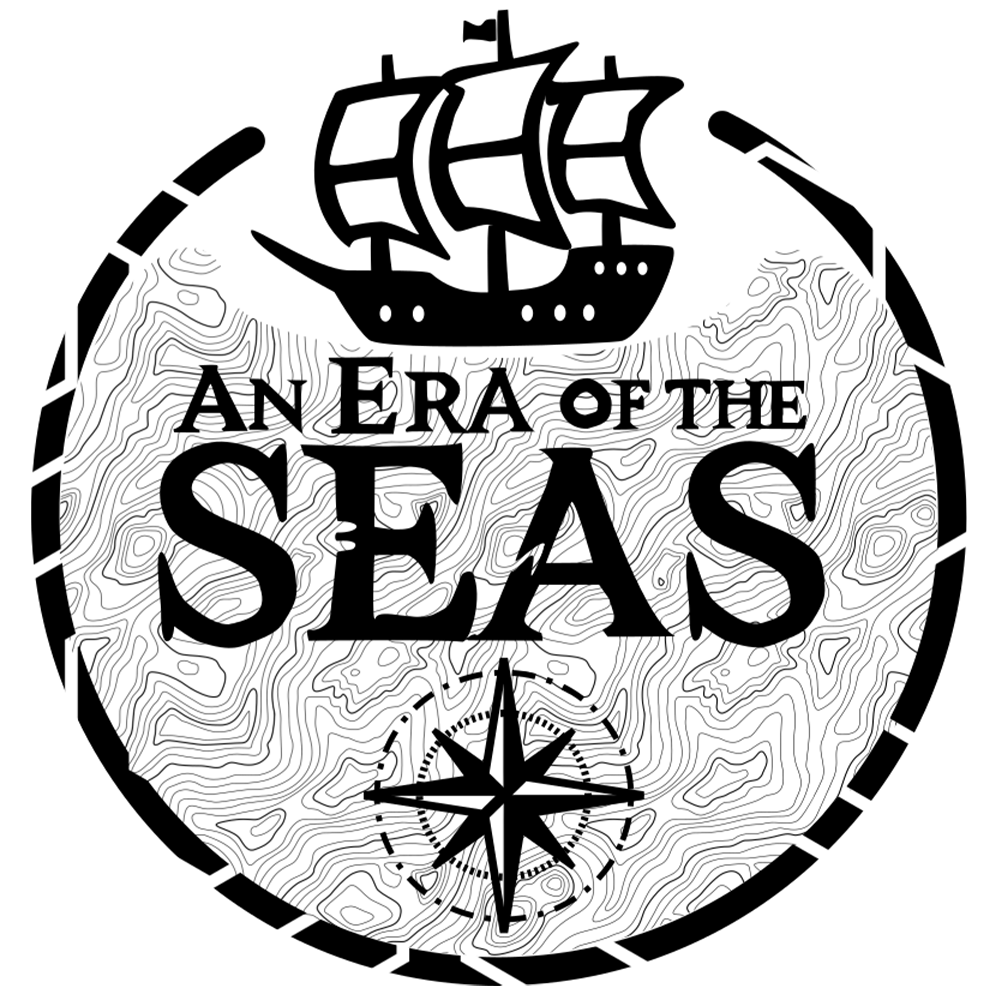
\includegraphics[width=3.5in]{AEotS Logo.png} \\
        \vspace{2cm}
        
\includegraphics[width=4in]{logo text.png}
    \end{minipage}
}
\date{}















\begin{document}

\maketitle

\vfill
\begin{center}
    \textbf{Lin Jérôme}\\
    \textbf{Ben Abdallah Achref}\\
    \textbf{Bruno Ethan}\\
    \textbf{Devin Joseph}\\
    \textbf{Class : A1}
\end{center}










\newpage
\thispagestyle{empty}
\addtocounter{page}{-1}
\null















\newpage
\section*{Introduction}\hfill

The project \textit{An Era of the Seas} stands out for its ambition to create a captivating maritime world where adventure and exploration lie at the heart of the gaming experience. Developed by the passionate team of \textbf{Dream Chasers}, this visual novel invites players to immerse themselves in the fascinating universe of sailing, through epic quests and strategic challenges.\\

\textit{An Era of the Seas} places players in the shoes of a captain who must traverse uncharted islands, confront formidable foes, and rebuild a family legacy. While navigating the Shattered Seas, players will discover a living, evolving environment designed to bring new life to every exploration. The realistic navigation system, ship upgrades, and crew management are all elements that enrich the experience while immersing the player in an authentic and intriguing world.\\

Through this project, \textbf{Dream Chasers} aims to deliver a complete and immersive gaming experience, combining technological innovation with narrative depth. The team strives to push the boundaries of video game development to offer a unique adventure, rich in discovery and strategy, that will captivate fans of exploration and piracy games.

\newpage
\subsection*{Summary}
\tableofcontents















\newpage
\section{Origin and nature of the Project}
\subsection{Origin}\hfill

The project for the game \textit{An Era of the Seas} stems from a shared interest among team members in video games and software development. It involves combining knowledge in computer science and video game development to create a captivating experience. This project is an opportunity to put acquired knowledge into practice by creating a tangible product.\\

Developing a game is an opportunity to acquire skills in various fields, from programming to graphic design, as well as sound production. Each member can contribute their unique skills, enriching the collective experience.\\

The rise of the video game industry and its growing importance in various domains such as education and entertainment also influenced the decision to create a game. It is an opportunity to immerse ourselves in the dynamic and ever-evolving video game sector.















\subsection{Game Information} 
\subsubsection{Beginning and Story of the Main Character}\hfill

\textit{An Era of the Seas} is a game where the maritime environment plays a central role. Players will embody the son of a great and powerful merchant who wielded significant influence and control over the seas. One day, he receives a letter informing him that his father perished during a mysterious expedition. Determined to uncover the truth, he begins his journey as a captain, aiming not only to restore his father's legacy but also to discover what truly happened.\\

As he explores the diversity of islands, he embarks on a voyage to become a great hero, just as his father was, while seeking answers to his own questions.



\subsubsection{Player Objectives}\hfill

Players will navigate and explore the islands of the Shattered Seas. To begin this adventure, the captain starts with nothing more than a small wooden boat he found on the shore. He must also explore eight different islands. Players will begin on the first island, where they will discover the main features, functionalities, and backstory of the son of the great merchant. Here, they will uncover the path to achieving the captain's ultimate goal.\\

The captain must travel to and reach each island to recover his father's scattered treasures and take control of the Shattered Seas. After exploring the first seven islands, the captain will finally be able to complete his journey on the last island, where the most challenging obstacles and trials await.



\subsubsection{Game Features}\hfill

This game offers unique features tied to its environment.

\paragraph{Main Quest}\hfill

This game is story-driven. Players will experience the captain's tale and be fully immersed in the game's maritime universe. Through the main quest, players will follow the captain's journey.

\paragraph{Immersive Navigation System}\hfill

The ship uses either wind or oars for navigation, depending on the ship's level and the crew's capabilities. This means starting with oars for lower-level ships, then progressing to harnessing the wind's direction, adjusting sails, and using the rudder for higher-level ships. To help the captain locate himself and chart a course to a specific destination, he will use a map and a compass.

\paragraph{Ship Maintenance and Upgrades}\hfill

The player's ship can be upgraded as they progress through the main quest. When the ship is damaged, the player must repair it using materials to continue navigating the seas. They can purchase a basic ship from a vendor and enhance it with specific materials.

\paragraph{Crew Members}\hfill

Since the player assumes the role of a captain navigating the seas, they have their own crew. This crew consists of various members with diverse tasks who have been carefully recruited from towns and quests to assist the captain on his journey. Each member has specific stats. Therefore, it is advisable to assign them to the appropriate tasks that will benefit the captain's journey. For example, some crew members are better suited to handle the oars, while others are more adept at exploration.

\paragraph{Weapons}\hfill

To fight against enemies, the player has the option to use swords and rifles. Weapons can be found in treasure chests, but these are common and low-powered. It is recommended to purchase weapons from merchants in the towns to acquire those with better stats and deal more damage.

\paragraph{Sigils (Player Upgrades)}\hfill

Sigils are marks inscribed on the hand with the help of a mage located in the towns. These marks enhance the player's abilities (speed, attack, etc.). They can be obtained by collecting them in treasure chests or by purchasing them from the mage. The mages have invested significant time and effort into creating the Sigils. As a result, Sigils sold by mages are much more effective and powerful than those found in nature. Therefore, buying Sigils from a mage provides significantly higher stats than those found in treasure chests. Of course, this quality comes at a cost, as these Sigils are far more expensive than those discovered in nature.

\paragraph{Towns}\hfill

Each island has its own town, where various types of merchants can be found:
\begin{itemize}
    \item \textbf{Boat Salesman:} They offer their exquisite creations, from small boats to massive ships. Depending on the island, these dealers provide better hulls and ship upgrades.
    \item \textbf{Armorer:} They sell high-quality swords and rifles to face enemies.
    \item \textbf{Mages:} They use their mystical magic to inscribe a Sigil that the captain owns or has purchased. They also sell their own more powerful Sigils.
    \item \textbf{Materials Seller:} They sell materials such as Pure Water Droop, Wood and Steel used for upgrading player's equipment.
\end{itemize}

\paragraph{Combat (PvE)}\hfill

In this adventure, the captain's journey is far from peaceful; he will encounter various enemies, both on the islands and across the seas. To defend himself and attack enemies, weapons, Sigils, and the crew will be useful in battle. As with the seas, the ship can also attack, and the crew members are crucial in this regard. Therefore, the stats of weapons, Sigils, the crew, and the ship are essential for dealing damage and withstanding enemy attacks.

\paragraph{Multiplayer}\hfill

This game features a multiplayer mode where players can choose to play mini-games with friends such as Treasure Hunt and Boat Race. In this mode, no advantages related to progress or items from the single-player mode are granted to the player.

\paragraph{Fishing}\hfill

A fun mechanic allowing the player to catch fish, which are useful for food and it can be used in large bodies of water such as lakes.



\subsection{Tools}
\subsubsection{Team Management Tools}\hfill

To communicate effectively on various aspects of game development among team members, it is crucial to have a dedicated tool. In this regard, a Discord server is particularly useful. It allows the team to easily communicate and organize discussions into different channels based on specific development topics.\\

Additionally, task management is essential for keeping the project on track and monitoring progress. A to-do list can be very helpful in this area, providing a clear overview of tasks to be completed. Microsoft To Do is an excellent solution for this. Tasks can be assigned to a team member, and a deadline can be set for each task. This allows team members to be aware of what needs to be done, the deadlines, and helps maintain their productivity.



\subsubsection{Game Development Tools}\hfill

Dream Chasers uses GitHub to work efficiently as a group on the project. It allows the team to track changes made to the game's code, ensuring that everyone is working on the latest version without overwriting others' work.\\

The game is coded in C\# (Csharp) for several reasons. C\# is an object-oriented programming language, a useful feature for games, and C\# is also commonly used in game engines like Unity.\\

For the IDE (Integrated Development Environment), the team uses Rider by JetBrains because it offers various advantages. It is specifically designed for .NET development (dotnet). Here, the team uses .NET Core 7 to develop the game. Rider's debugging tool is very powerful, making it easier to identify issues in the code through step-by-step debugging and variable monitoring. Additionally, Rider provides a Unity editor and is generally faster than other IDEs like Visual Studio.\\

The game engine used is Unity, as mentioned earlier, for many reasons. It provides an accessible user interface that simplifies project management for developers. With Unity, the game can be supported on multiple platforms, meaning it will run smoothly whether the player is using Windows, macOS, or Linux. It offers a variety of tools and features for the game's 3D environment, including an integrated physics engine.



\subsection{Official Website}\hfill

The official website of the game can be accessed at: \url{https://dream-chasers.odoo.com}. It provides information about Dream Chasers and the game with official download links.














\newpage
\section{Study Objective}
\subsection{Interests and Objectives}\hfill

The main objective of the project is to create an immersive gaming experience, with a captivating story and engaging mechanics. Through this project, the team members will be able to apply the knowledge and concepts they have learned in a real and creative context. The game development process allows the team to overcome technical challenges and encourages them to develop practical problem-solving skills.





\subsection{Shared Benefits}\hfill

This project offers numerous benefits for teamwork.

Working with others fosters effective communication between team members, a crucial skill in the professional world. Through frequent discussions, team members develop the ability to clearly express their ideas, listen to feedback, and adapt to different perspectives.\\

Moreover, teamwork encourages better coordination, with management of task dependencies. Each team member can specialize in certain tasks, such as programming, game design, and audio engineering, which enhances productivity and efficiency. Task division also allows the project to progress more quickly, as tasks can be completed simultaneously.\\

Finally, teamwork leads to more innovative and creative solutions. Brainstorming can generate a variety of ideas, resulting in more original and unique game concepts and mechanics.





\subsection{Individual Benefits}\hfill

There are also many personal benefits to participating in this type of project.\\

Game development primarily allows developers to master specific technologies. For example, team members can focus on different aspects of game creation, such as game logic, physics engine, 3D design and animation, sound design, and more.\\

Additionally, team members will inevitably encounter technical challenges, obstacles, and problems throughout the process. Problem-solving strengthens problem-solving abilities, which is a crucial skill in any computer science career. Overcoming these challenges also boosts confidence and helps members become more adaptable.\\

In a collaborative project, each member must take on responsibilities. They are accountable for the quality and timeliness of their work. This can enhance the sense of autonomy and ownership. They must ensure that their contributions meet the team's expectations and deadlines, which helps in gaining independence.\\

Participating in a group project requires good time management. This means learning to balance personal work with the needs of the group. Team members must plan and prioritize their tasks, ensuring they contribute to the progress of the project.\\

Finally, working in a group on a game project allows members to acquire technical communication skills. Members must clearly explain ideas, solutions, and complex code to others, ensuring that everyone understands. This ability to communicate technical details in an accessible way is a very useful skill, one that will be frequently required in the professional world.















\newpage
\section{Company}
\subsection{Dream Chasers}\hfill

The company is called \textbf{Dream Chasers}, a name that reflects the company's spirit, in pursuit of creating an experience that turns the wildest dreams into reality. The company believes that games are not just mere entertainment; they are a gateway to new worlds, adventures, and the realization of fantastic ideas. The company's name is a tribute to those who dream and those who wish to chase those dreams.





\subsection{Specificities}\hfill

Dream Chasers stands out for its ability to blend technical skills with artistic expression. The company is dedicated to developing games that engage players not only intellectually, but also emotionally. The team is made up of enthusiastic developers, designers, and storytellers who view game creation as a form of art, combining cutting-edge technology, rich narratives, and immersive environments.\\

Dream Chasers' distinctive methodology is characterized by meticulous attention to detail, covering everything from gameplay mechanics to evocative music that enhances each scene. The company aspires to create not just games, but deep experiences that leave a lasting impression on players, encouraging them to reflect on their journey long after completing the game.\\

Furthermore, Dream Chasers prioritizes collaboration and innovation within its company culture. An atmosphere is cultivated to allow creativity to thrive, providing each team member with the opportunity to influence the trajectory of projects. This spirit of collaboration fosters new perspectives and continuous experimentation, ensuring that every game developed is a unique adventure.





\subsection{Field of Activity}\hfill

Dream Chasers operates in the dynamic field of video game development, but its scope extends beyond conventional gaming. The main goal lies in creating narrative-driven adventure games while exploring opportunities in educational technologies and virtual reality experiences.\\

Dream Chasers' aim is to create games that both educate and entertain, using interactive storytelling to address important themes such as environmental awareness, historical narratives, and personal growth. The company recognizes the potential of video games as effective learning and development tools, committing to integrate these elements into its projects as it moves forward.





\subsection{About the Game and the Company}\hfill

With this game, Dream Chasers engages players by asking if they have ever wondered what pirates did in the distant past. Players can feel a sense of nostalgia for the history of sailing and plundering in the Caribbean. This is why the team works closely with the Nostalgic Pirates Association (NPA) to develop this game, which aims to offer a refreshing reminiscence of the atmosphere and piracy of the 18th-century Caribbean. It will bring to life all the captains who lived during that era. Nostalgic pirates are invited to ask themselves if there is a more fulfilling way of life than sharing a drink with friendly crewmates on deck. Together, they can breathe the salty sea air, discover enchanting and unexplored islands, sail the seven seas, and embark on the search for magnificent treasures.\\

At Dream Chasers, there is a genuine commitment to addressing the concerns of the nostalgic pirate spirits, which is why the company helps those who can no longer pursue their dreams to experience them through a visual novel with the game \textit{An Era of the Seas}, designed for dreamers of the seas.















\newpage
\section{Task Distribution}
\begin{table}[h]
    \centering
    \begin{tabular}{|>{\columncolor{pastelblue!60}}l|c|c|c|c|}
        \hline
        \rowcolor{pastelblue!60}
        \textbf{Tasks} & \textbf{Jérôme} & \textbf{Achref} & \textbf{Ethan} & \textbf{Joseph}\\
        \hline
        Menu \& UI & \cellcolor{blue}R &  & \cellcolor{cyan}S &\\
        \hline
        Water Simulation & & & \cellcolor{blue}R & \cellcolor{cyan}S\\
        \hline
        Weather Simulation & & \cellcolor{blue}R & \cellcolor{cyan}S &\\
        \hline
        Movements (boat, player...) & & & \cellcolor{cyan}S & \cellcolor{blue}R\\
        \hline
        AI Movements (enemies, movements, attacks) & & \cellcolor{blue}R & & \cellcolor{cyan}S\\
        \hline
        Map & \cellcolor{cyan}S & & \cellcolor{blue}R &\\
        \hline
        Localization System (map, compass...) & & \cellcolor{cyan}S & & \cellcolor{blue}R\\
        \hline
        Item Statistics & \cellcolor{blue}R & & & \cellcolor{cyan}S\\
        \hline
        Fishing System & \cellcolor{cyan}S & \cellcolor{blue}R & &\\
        \hline
        Hunger System & & \cellcolor{cyan}S & \cellcolor{blue}R &\\
        \hline
        Network & \cellcolor{blue}R & \cellcolor{cyan}S & &\\
        \hline
        Multiplayer & \cellcolor{cyan}S & & & \cellcolor{blue}R\\
        \hline
        Story (Lore) & & & \cellcolor{cyan}S & \cellcolor{blue}R\\
        \hline
        Quests & & \cellcolor{cyan}S & \cellcolor{blue}R &\\
        \hline
        Website & & \cellcolor{blue}R & & \cellcolor{cyan}S\\
        \hline
        Entity Design & & \cellcolor{blue}R & \cellcolor{cyan}S &\\
        \hline
        Entity Animations & \cellcolor{cyan}S & & \cellcolor{blue}R &\\
        \hline
        SFX & \cellcolor{blue}R & & & \cellcolor{cyan}S\\
        \hline
        Music & \cellcolor{blue}R & \cellcolor{cyan}S & &\\
        \hline
        Code Optimization & \cellcolor{blue}R & \cellcolor{blue}S & \cellcolor{blue}S & \cellcolor{blue}S\\
        \hline
        Language Correction & \cellcolor{cyan}S & & & \cellcolor{blue}R\\
        \hline
        Testing & \cellcolor{blue}R & \cellcolor{blue}R & \cellcolor{blue}R & \cellcolor{blue}R\\
        \hline
    \end{tabular}
\end{table}

\begin{itemize}
    \item \textcolor{blue}{R : Responsible}
    \item \textcolor{cyan}{S : Substitute}
\end{itemize}





\newpage
\begin{figure}[h]
    \caption*{\textbf{\uline{GANTT Chart}}}
    \centering
    
\includegraphics[angle=90, width=4.2in]{gant.png}
    \label{fig:my_image}
\end{figure}
\clearpage



















\section{Development Narrative}





\subsection{Menu and User Interface}
\paragraph{Objectives}\hfill

Before beginning development in Unity, preliminary research was conducted to understand how to design and implement menus and user interfaces within the engine. Several written guides and video tutorials were consulted to grasp the core principles of UI development. While the process initially seemed straightforward, it soon became clear that attention to detail would be essential—particularly in the visual design and placement of buttons and other UI elements. The main objective was to create a clean, intuitive interface that would enhance the gameplay experience without causing distraction or confusion.\\

In the final version of the project, the main menu includes options to choose between Solo and Multiplayer game modes. Within the Solo mode, the in-game interface provides the player with a health bar, defense bar, and hunger meter. Additionally, several functional buttons allow access to essential menus such as the inventory, character equipment, map, and item upgrade interfaces. These elements were designed to ensure quick navigation and seamless interaction, contributing to an overall user-friendly experience.\\

\paragraph{Implementation}\hfill

The design process began with the placement of buttons and the selection of a background image for the main menu. A suitable background, consistent with the game's maritime theme, was quickly found on Unity's Asset Store. However, locating appropriate pre-made buttons proved more challenging. After an extensive search, it was ultimately decided to create custom buttons using photo editing tools. These custom buttons were paired with a font that complemented the game's overall aesthetic to ensure visual consistency.\\

\begin{center}
    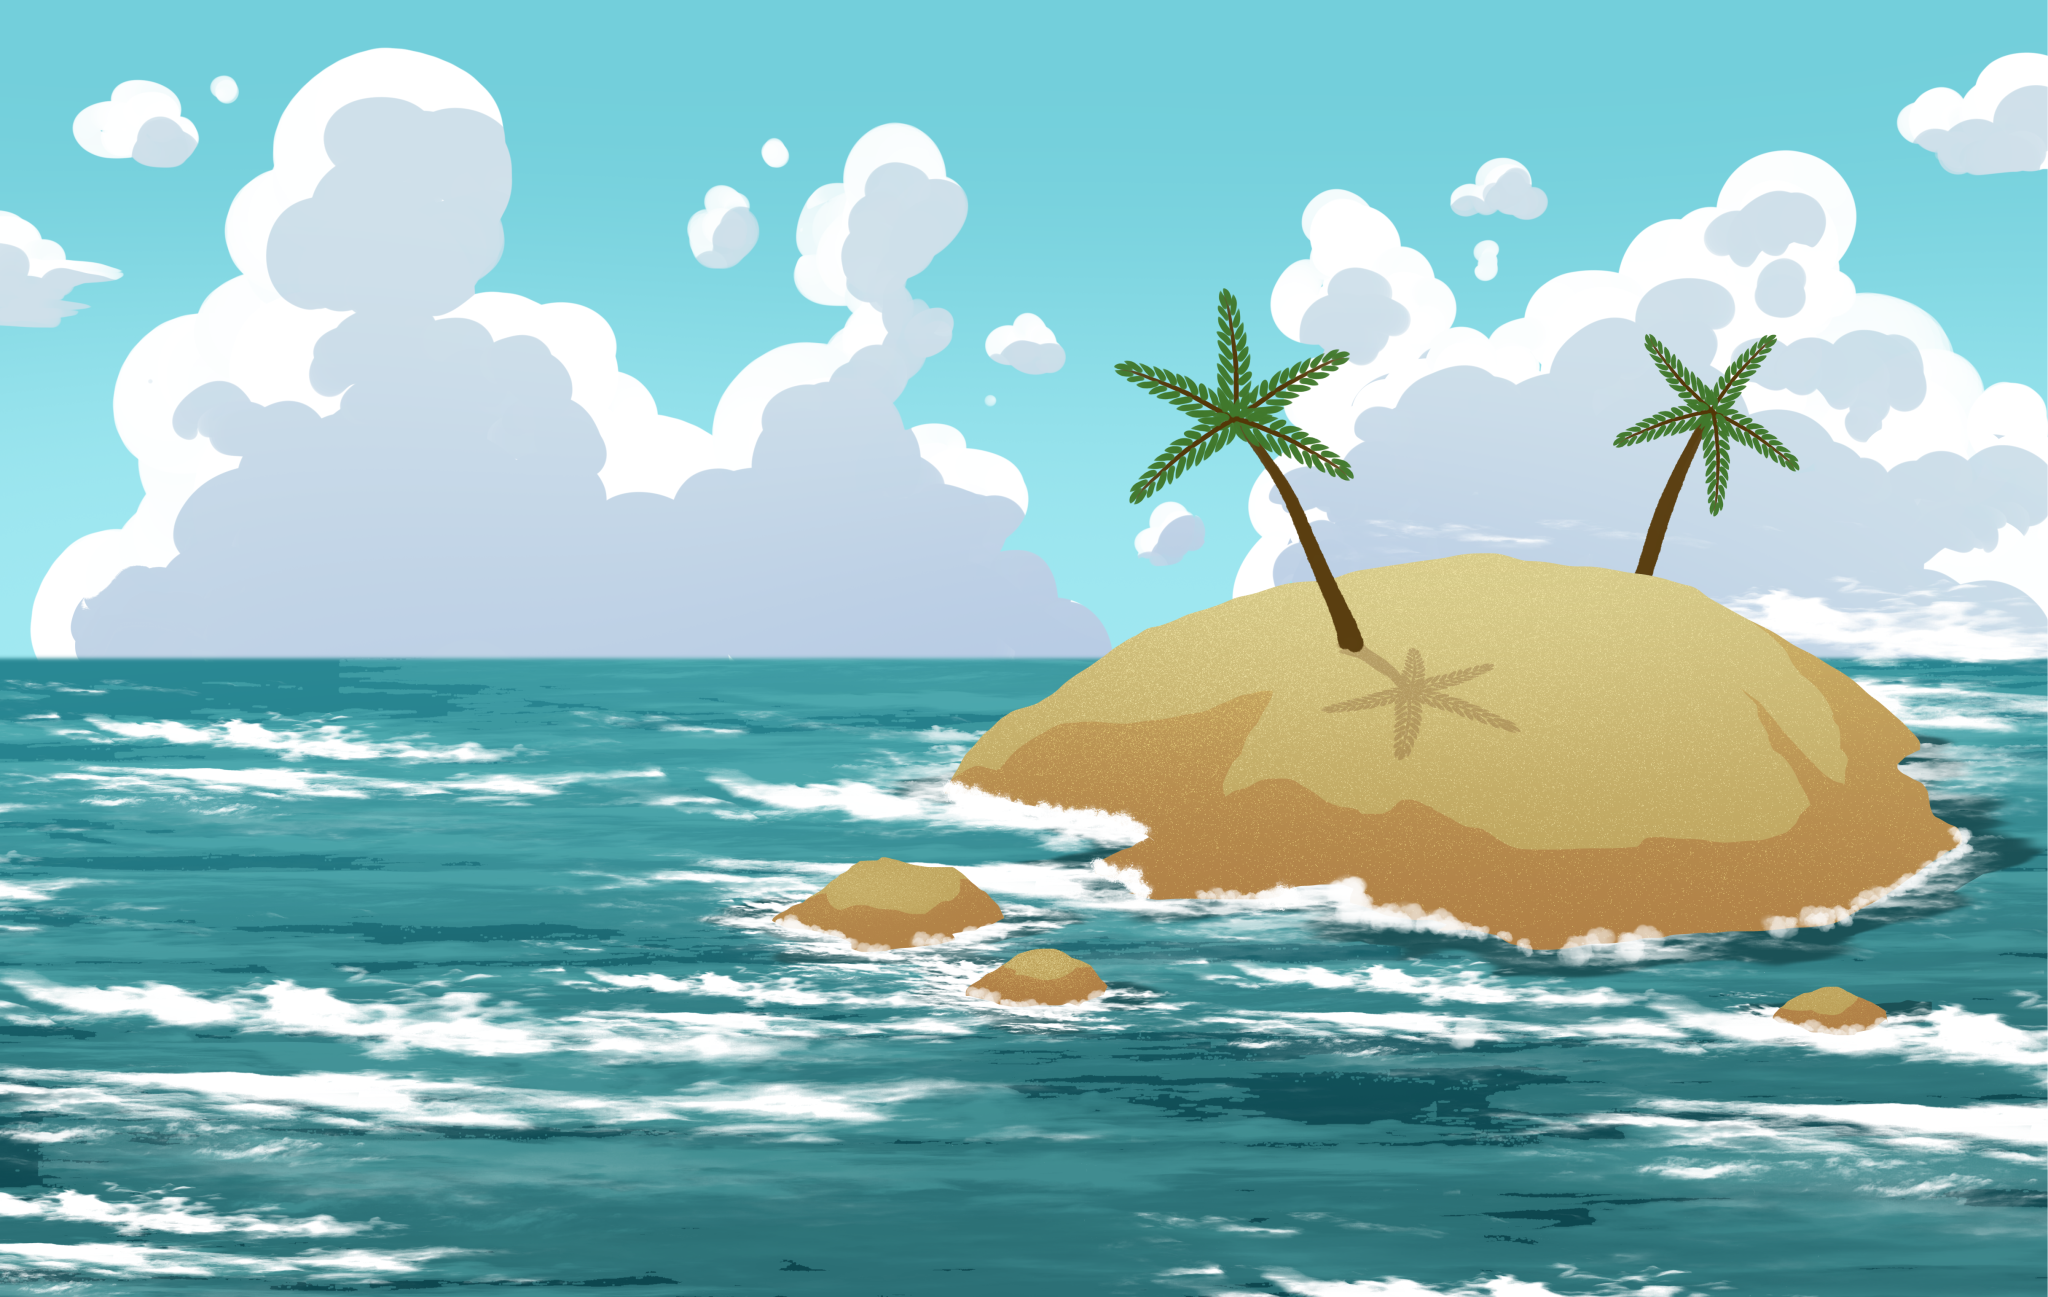
\includegraphics[width=2in]{Illustration/MenuUI/MainMenuBackground.png}
    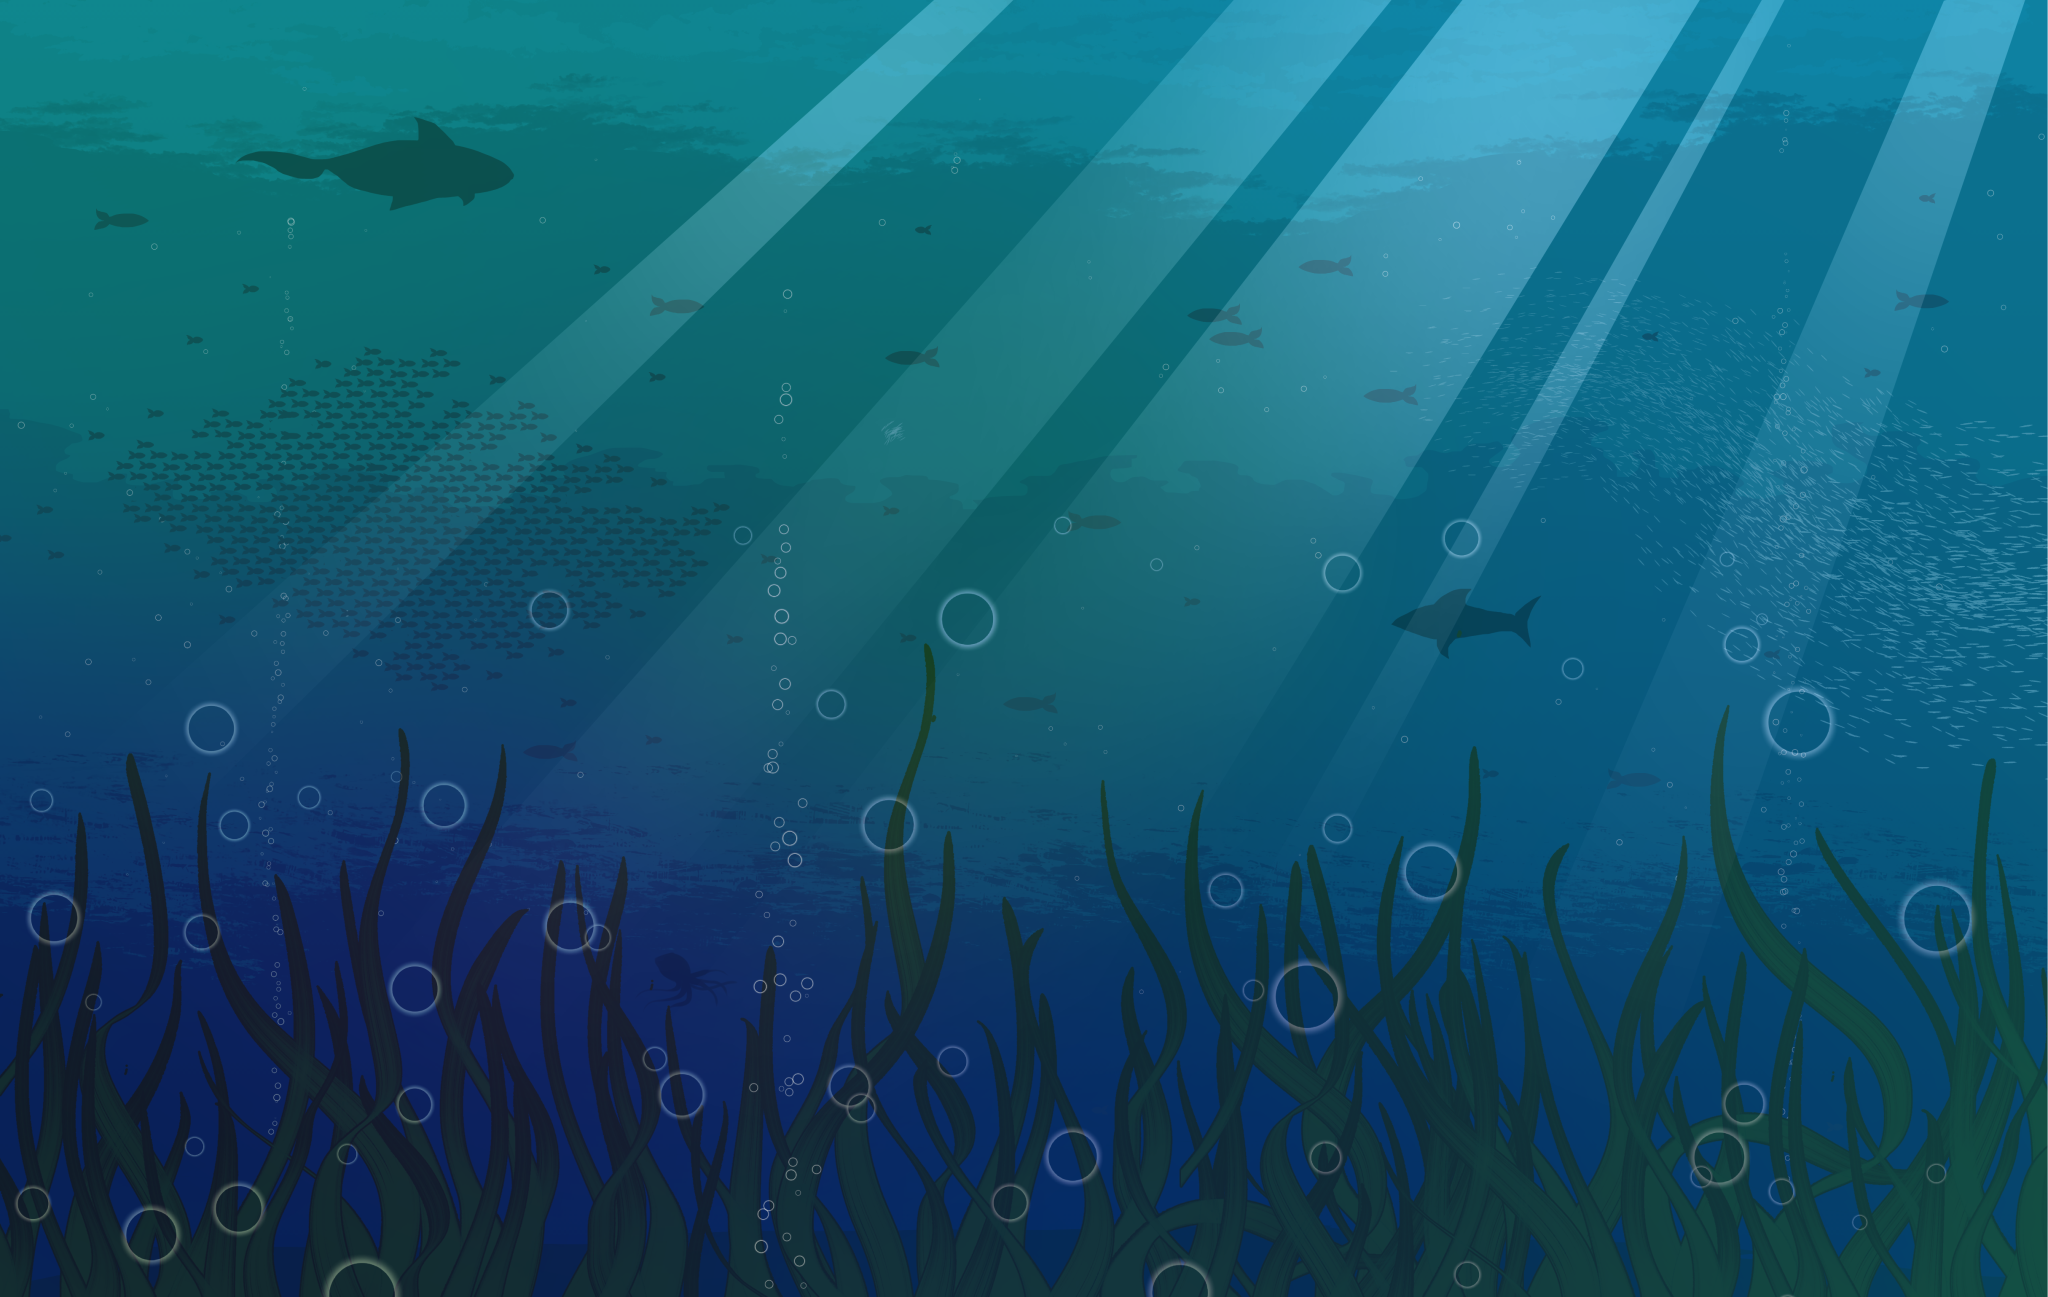
\includegraphics[width=2in]{Illustration/MenuUI/CreditsMenuBackgound.png}
\end{center}

Integrating the custom buttons into Unity introduced a learning opportunity. Initially, there was some confusion regarding how to replace Unity's default button sprites with custom images. Simply dragging and dropping image files into the editor did not yield the desired outcome. Further research revealed that the images had to be converted into sprite assets before they could be assigned. Once this process was understood, the custom designs were successfully implemented, giving the menu a unique and polished appearance.\\

\begin{center}
    
\includegraphics[width=2in]{Illustration/MenuUI/Button300x100.png}
    
\includegraphics[width=1in]{Illustration/MenuUI/BackpackButton.png}
    
\includegraphics[width=1in]{Illustration/MenuUI/HomeButton.png}
    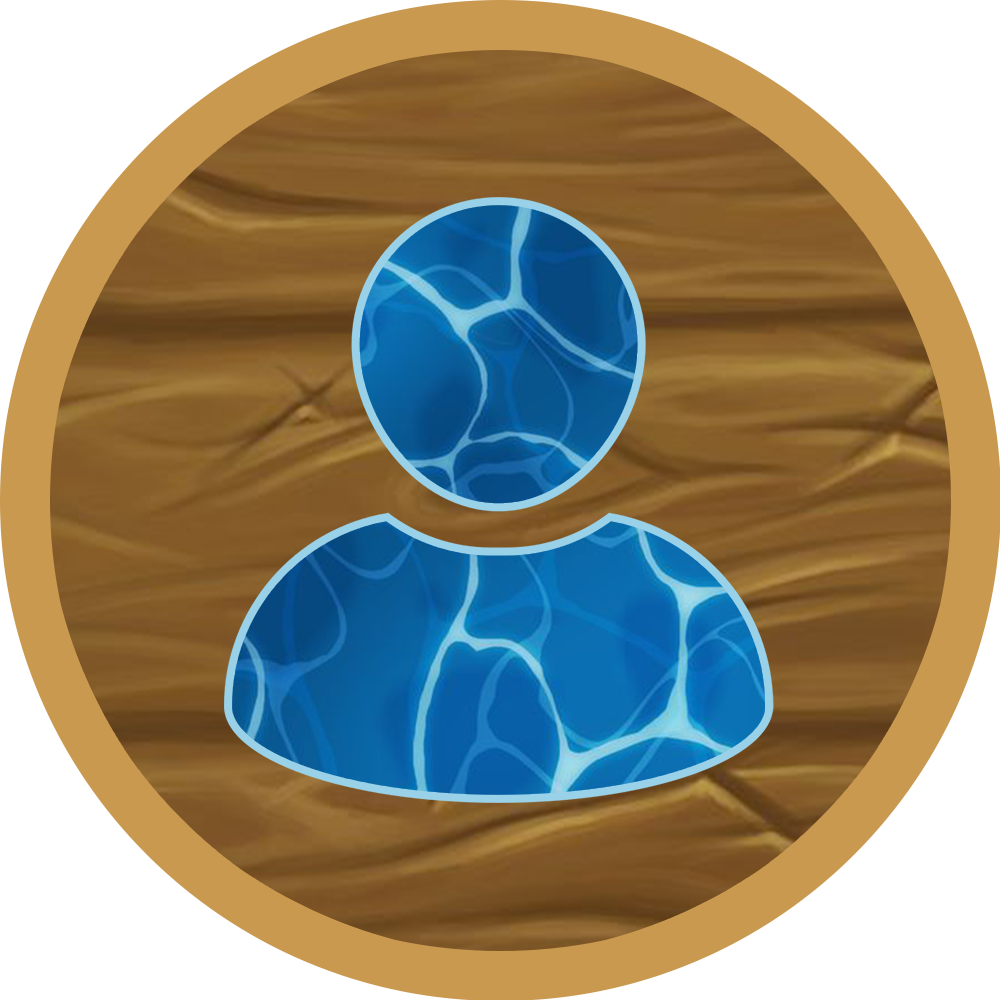
\includegraphics[width=1in]{Illustration/MenuUI/CharacterButton.png}
    
\includegraphics[width=1in]{Illustration/MenuUI/ReturnButton.png}
    
\includegraphics[width=1in]{Illustration/MenuUI/QuitButton.png}
    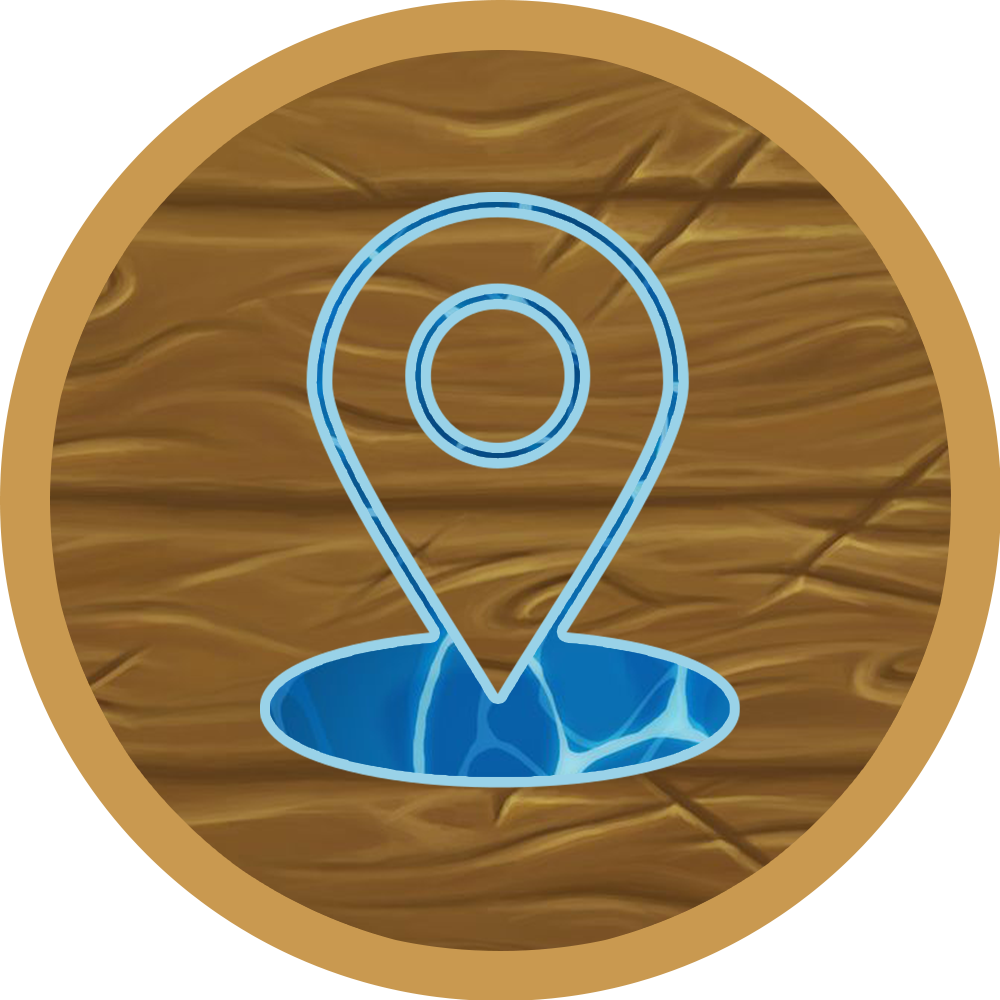
\includegraphics[width=1in]{Illustration/MenuUI/MapButton.png}
    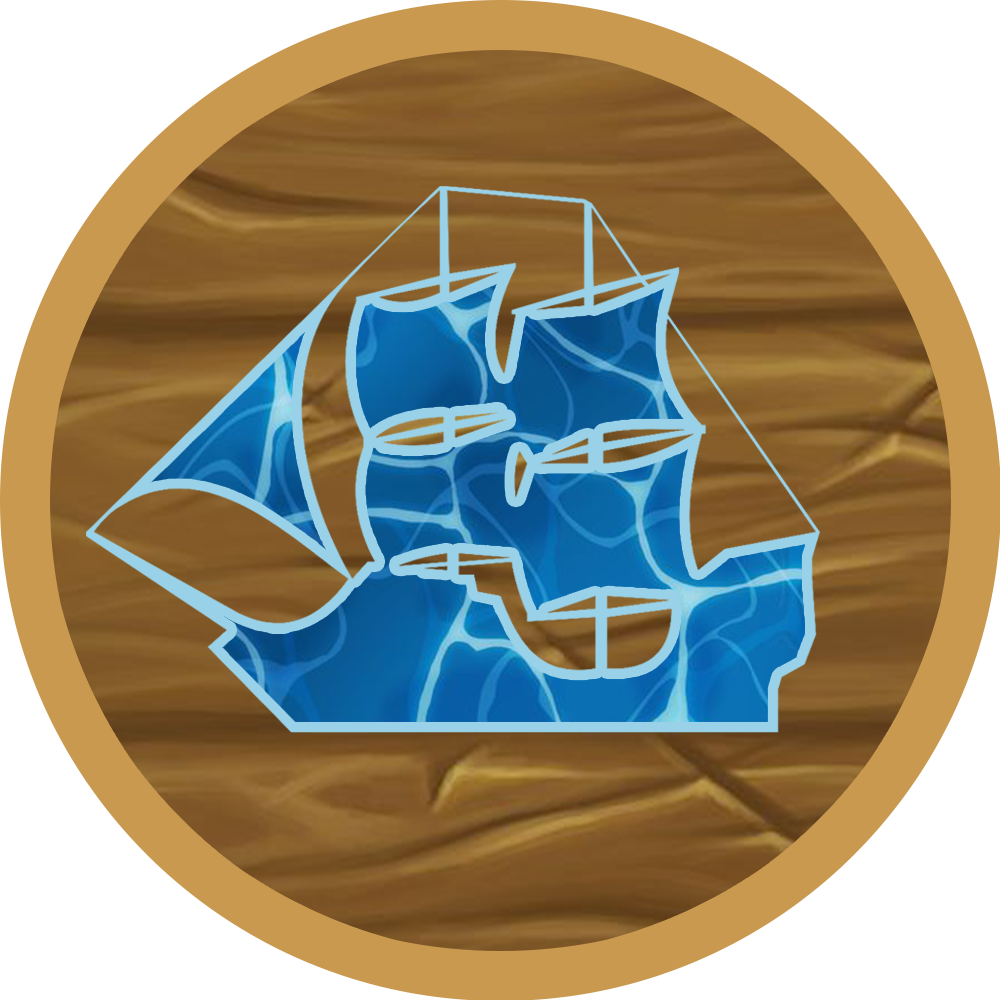
\includegraphics[width=1in]{Illustration/MenuUI/BoatButton.png}
\end{center}

Following the visual design, scripts were developed to handle user interactions within the menu. This included switching between canvases and toggling the visibility of various GameObjects based on player input. Unity's built-in UI system made this functionality relatively straightforward to implement, requiring minimal additional research.\\

The development of the inventory menu presented a significantly more complex challenge. This system needed to dynamically display items collected by the player in real time. A step-by-step video tutorial provided valuable guidance for implementing this feature. Building on that foundation, a dynamic data-binding system was created to handle item additions, removals, and updates based on player interactions. Each item had its own properties and visual representation, necessitating a flexible and extensible inventory structure.\\

Design considerations for the inventory included the creation of item icons, layout of inventory slots, and implementation of effective sorting mechanisms to maintain clarity and ease of use. Various Unity UI components—such as ScrollViews, Buttons, and TextMesh Pro—were utilized to enhance both functionality and visual appeal. This phase of development also required revisiting key C\# programming concepts to ensure accurate data handling and smooth system integration.\\

In addition to the inventory, the player's equipment menu was developed. This interface included a switch menu for changing equipped items and an upgrade menu for enhancing item attributes. These features were considerably easier to implement after completing the inventory system, as they built on similar logic and structures. It was also essential to ensure that changes made within these menus were correctly saved to the player's persistent data, maintaining consistency between sessions.

\paragraph{Results}\hfill

The development process resulted in a distinctive and immersive main menu, featuring custom-designed buttons and a visually coherent interface that aligned with the game's overall aesthetic. Implementing the UI provided valuable hands-on experience and a deeper understanding of Unity's interface tools and systems.\\

The inventory system, though more complex, was successfully implemented and functioned in real-time based on player actions. It provided a well-structured and intuitive interface that significantly improved user experience. The final UI was both functional and visually refined, contributing positively to the overall usability and enjoyment of the game.\\

\begin{center}
    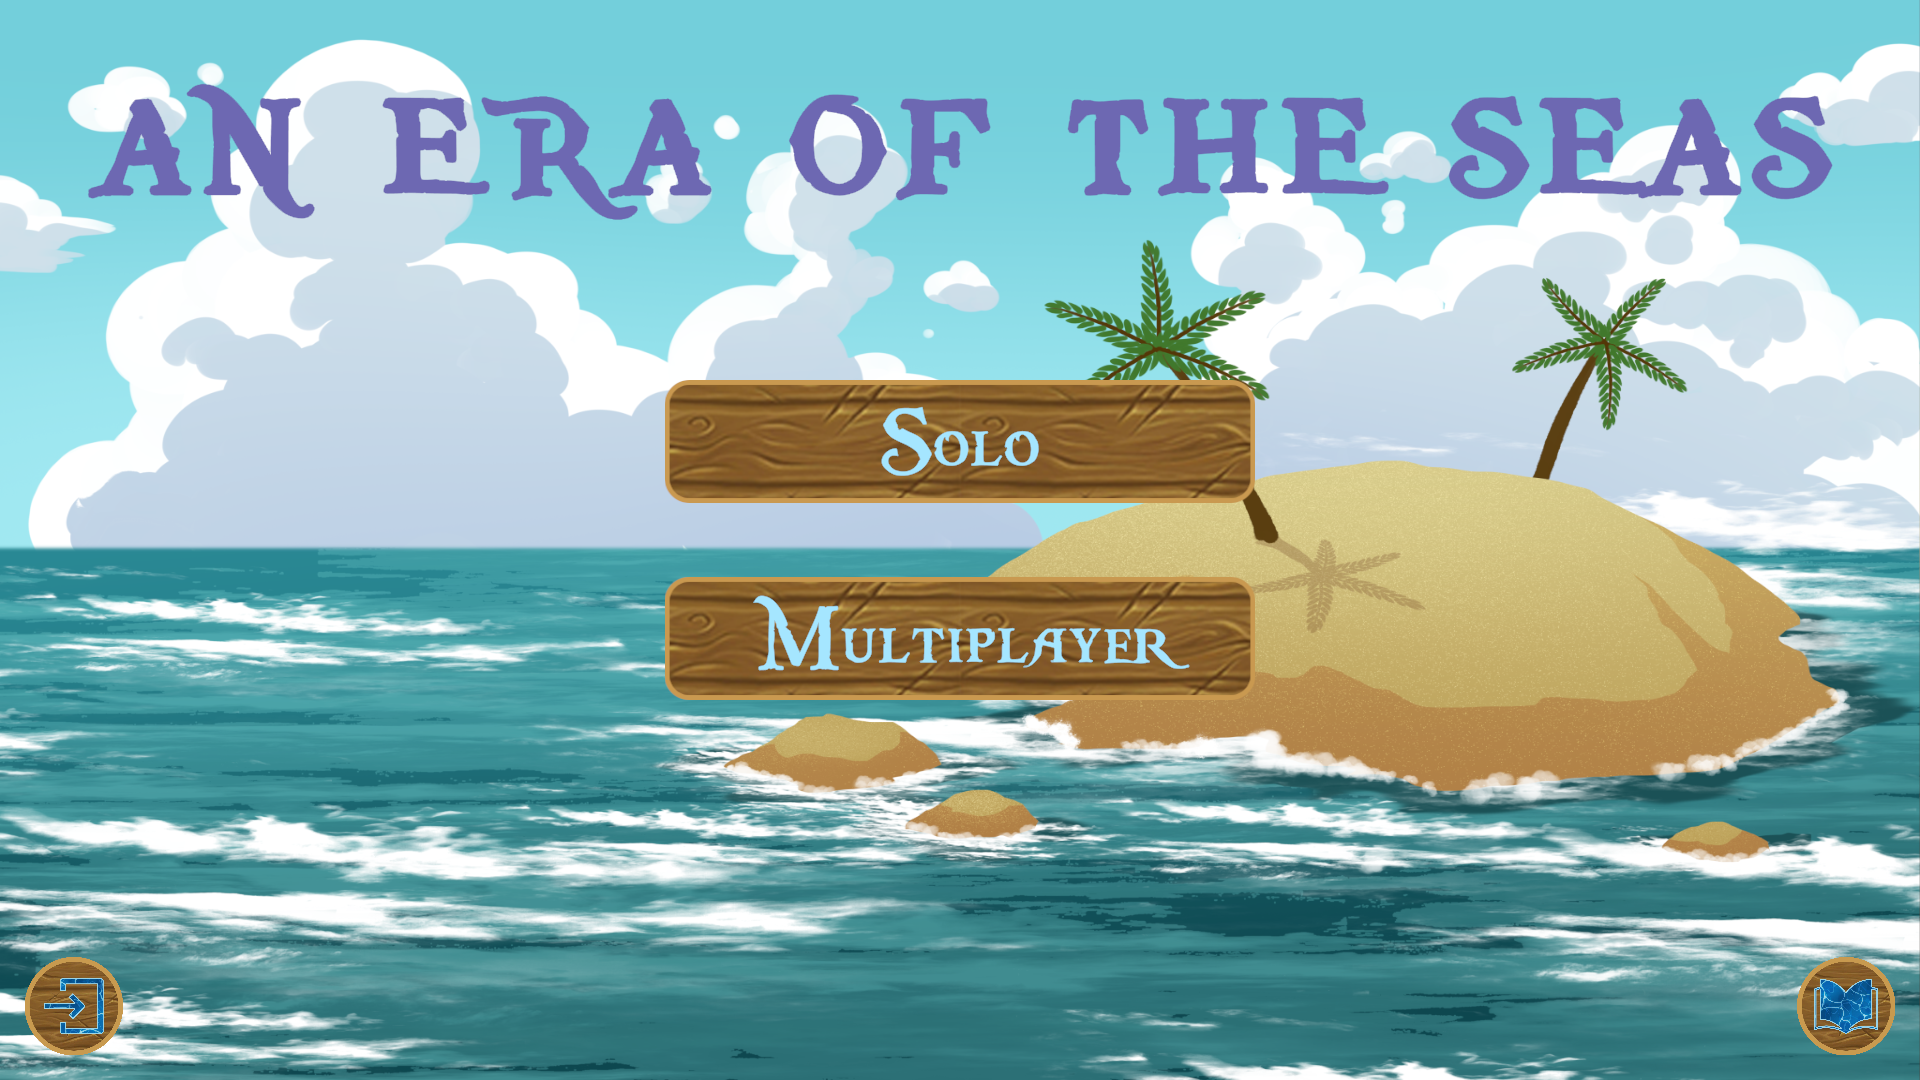
\includegraphics[width=5in]{Illustration/MenuUI/MainMenu.png}
\end{center}

In the final version, the player's user interface includes health, defense, and hunger bars, along with several key buttons: Settings, Inventory, Equipment, Map, a button to place the boat, and an Eat button. The Settings menu provides access to sub-menus including Equipment, Map, and Inventory. Additionally, players can adjust music and sound effects volume or exit the solo game to return to the main menu.\\

    
\begin{center}
    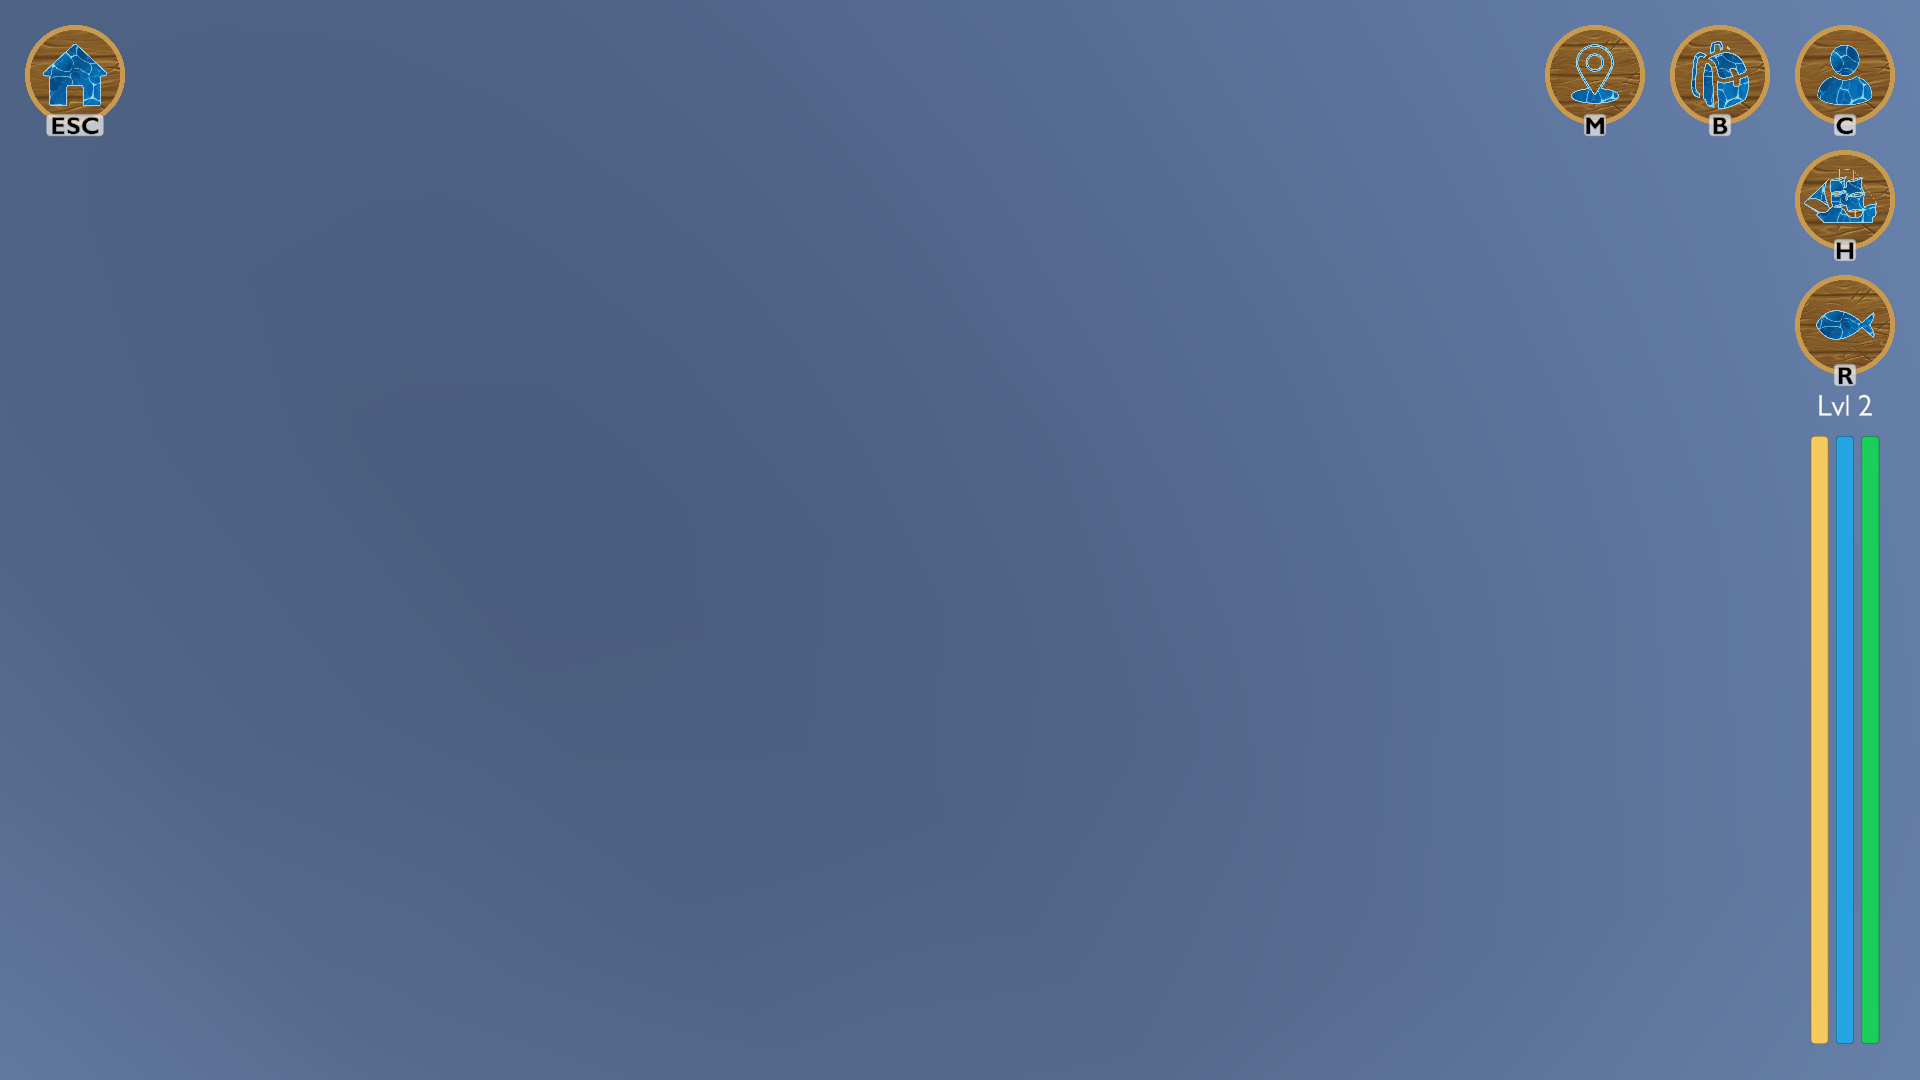
\includegraphics[width=5in]{Illustration/MenuUI/PlayerUI.png}
\end{center}

Within the Inventory menu, items are categorized into different types: Materials (such as coins, pure water drops, wood, steel, and fish), Weapons, Sigils, Boats, and Crew Members. When an item is selected, the player can view its statistics and, if applicable, upgrade it.\\

\begin{center}
    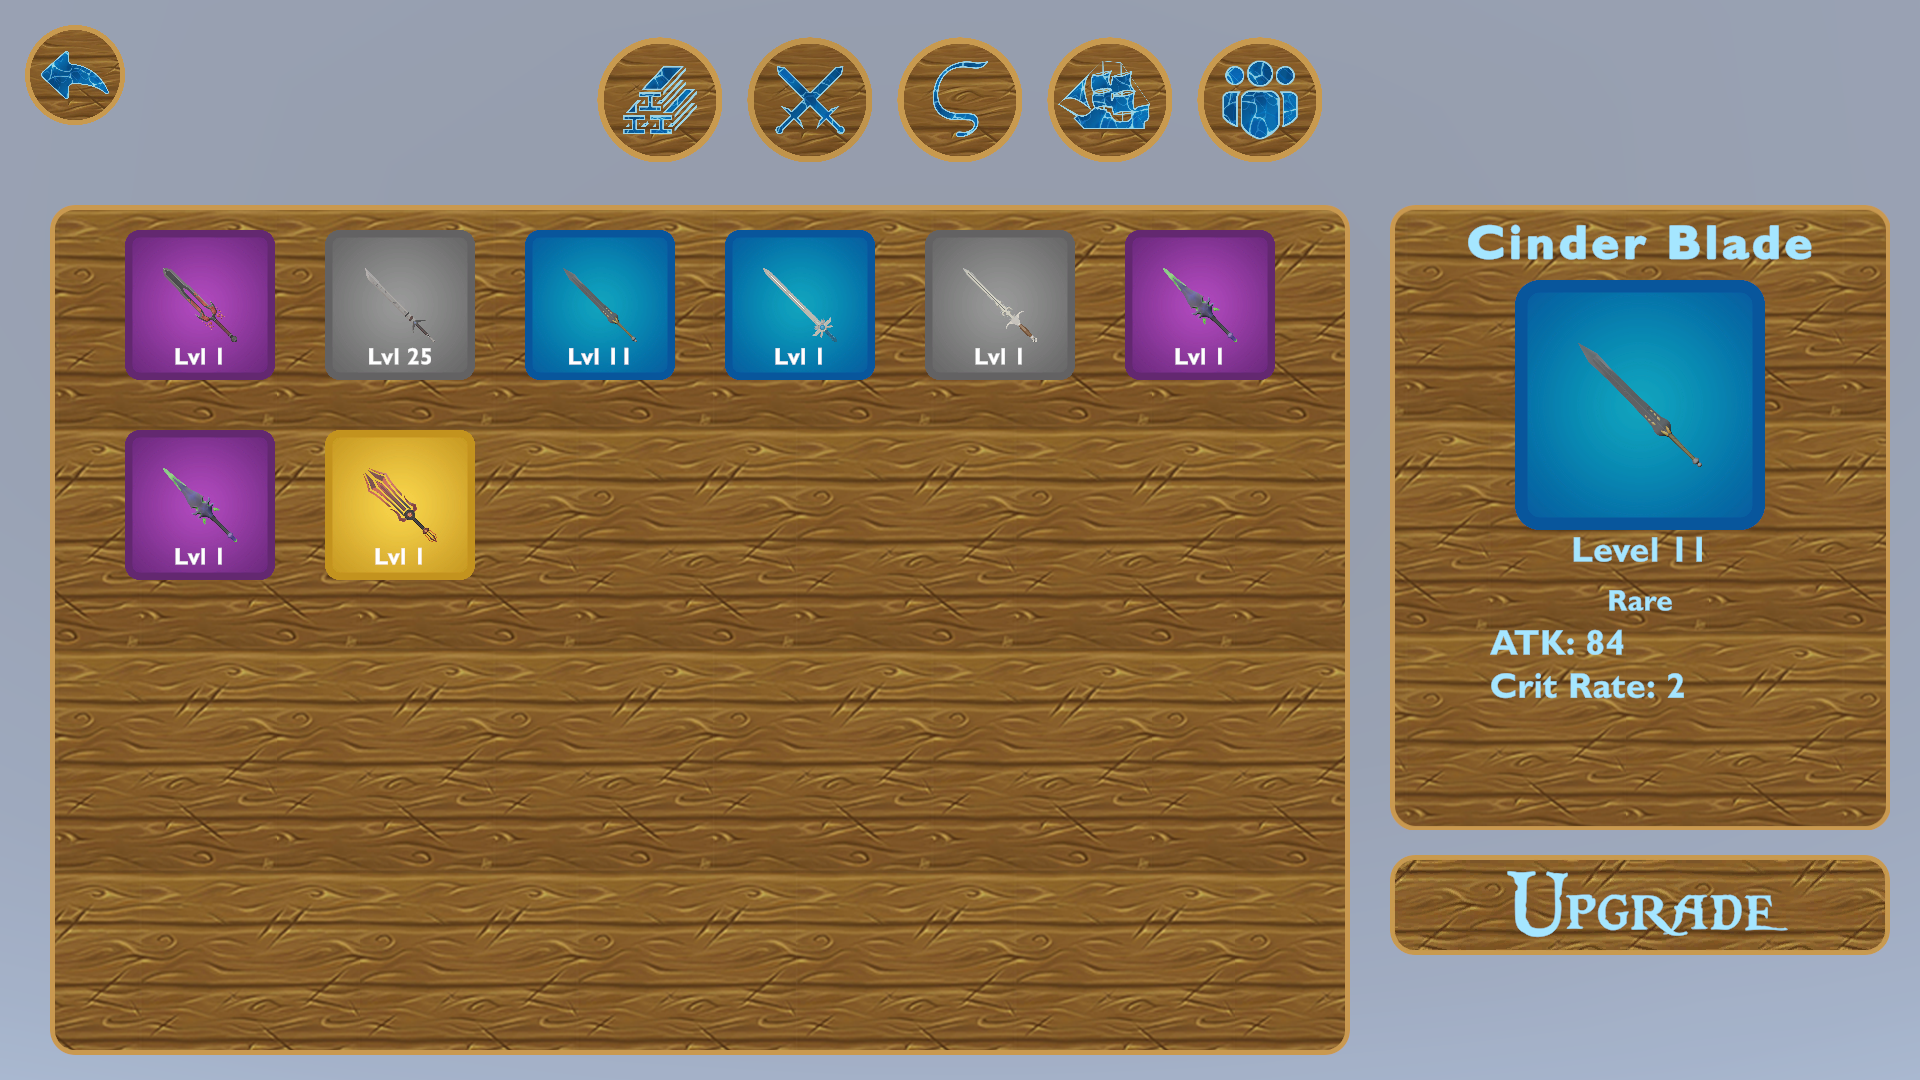
\includegraphics[width=5in]{Illustration/MenuUI/Inventory.png}
\end{center}

In the Upgrade menu, players can enhance their items using specific resources like coins, pure water drops, and sometimes steel or wood depending on the item. Upgrade options allow the player to increase item levels by increments of 1, 2, 5, or 10, offering flexibility in progression.\\

\begin{center}
    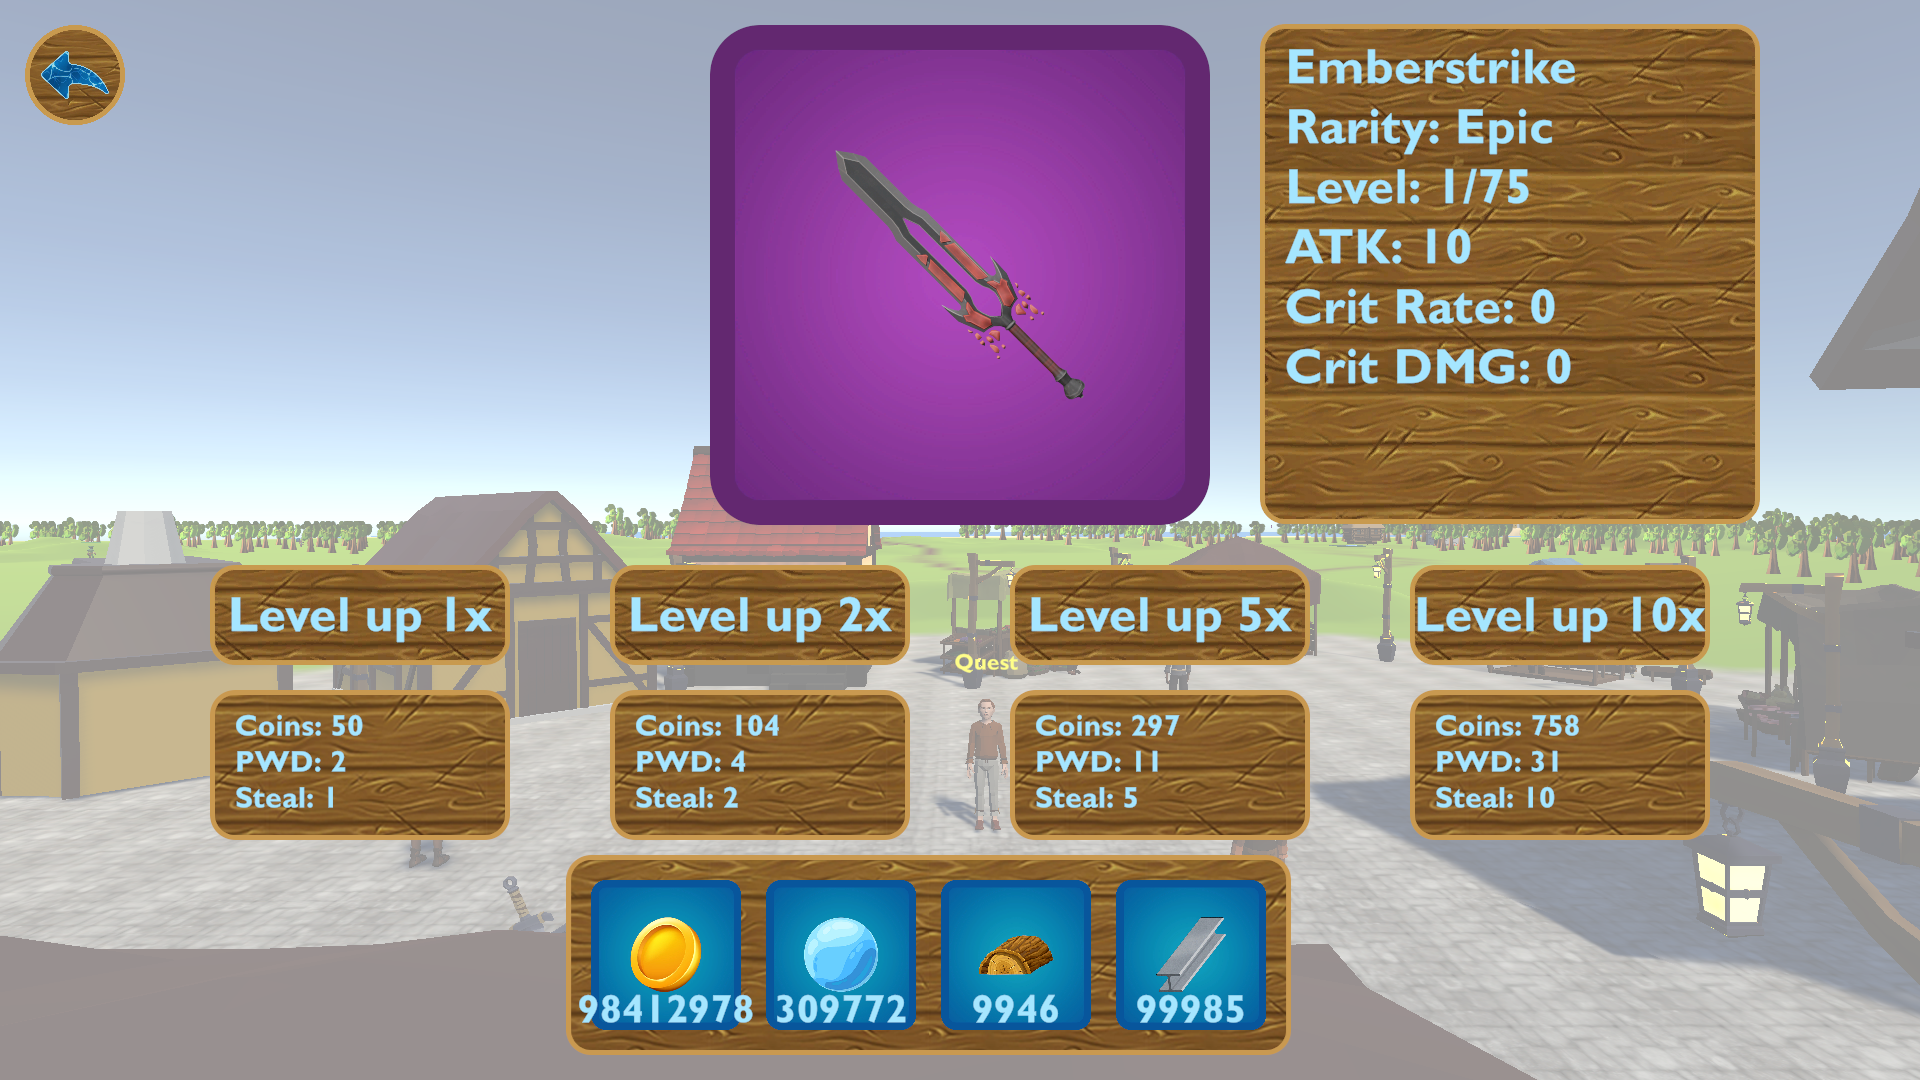
\includegraphics[width=5in]{Illustration/MenuUI/UpgradeMenu.png}
\end{center}

The Equipment menu displays the player's current statistics and allows character progression. It shows the currently equipped Boat, Sigil, Weapon, and Crew Member. Players can either upgrade these equipped items or swap them for alternatives in their inventory using the Switch menu. The Switch menu displays all compatible items available for each slot. When the player selects an item, it is automatically equipped, replacing the previous one.

\begin{center}
    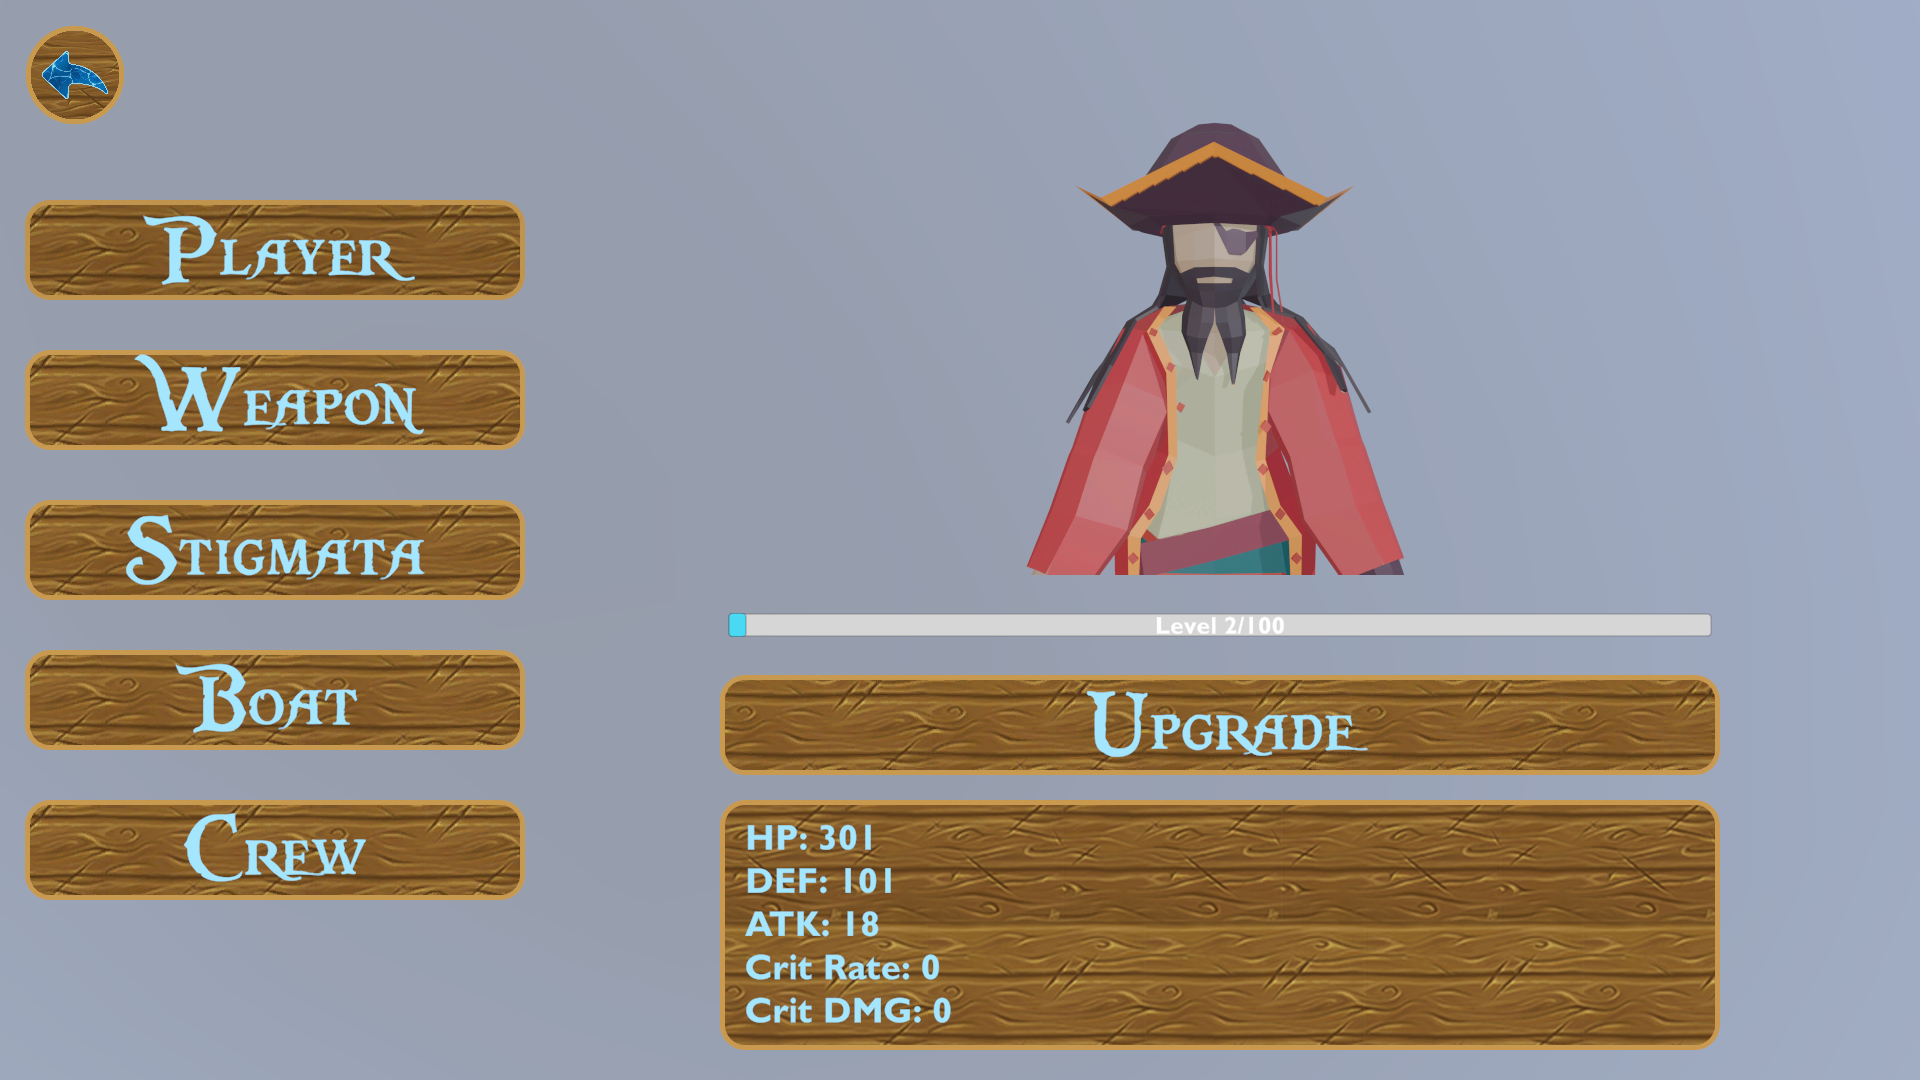
\includegraphics[width=5in]{Illustration/MenuUI/EquipmentMenu.png}
    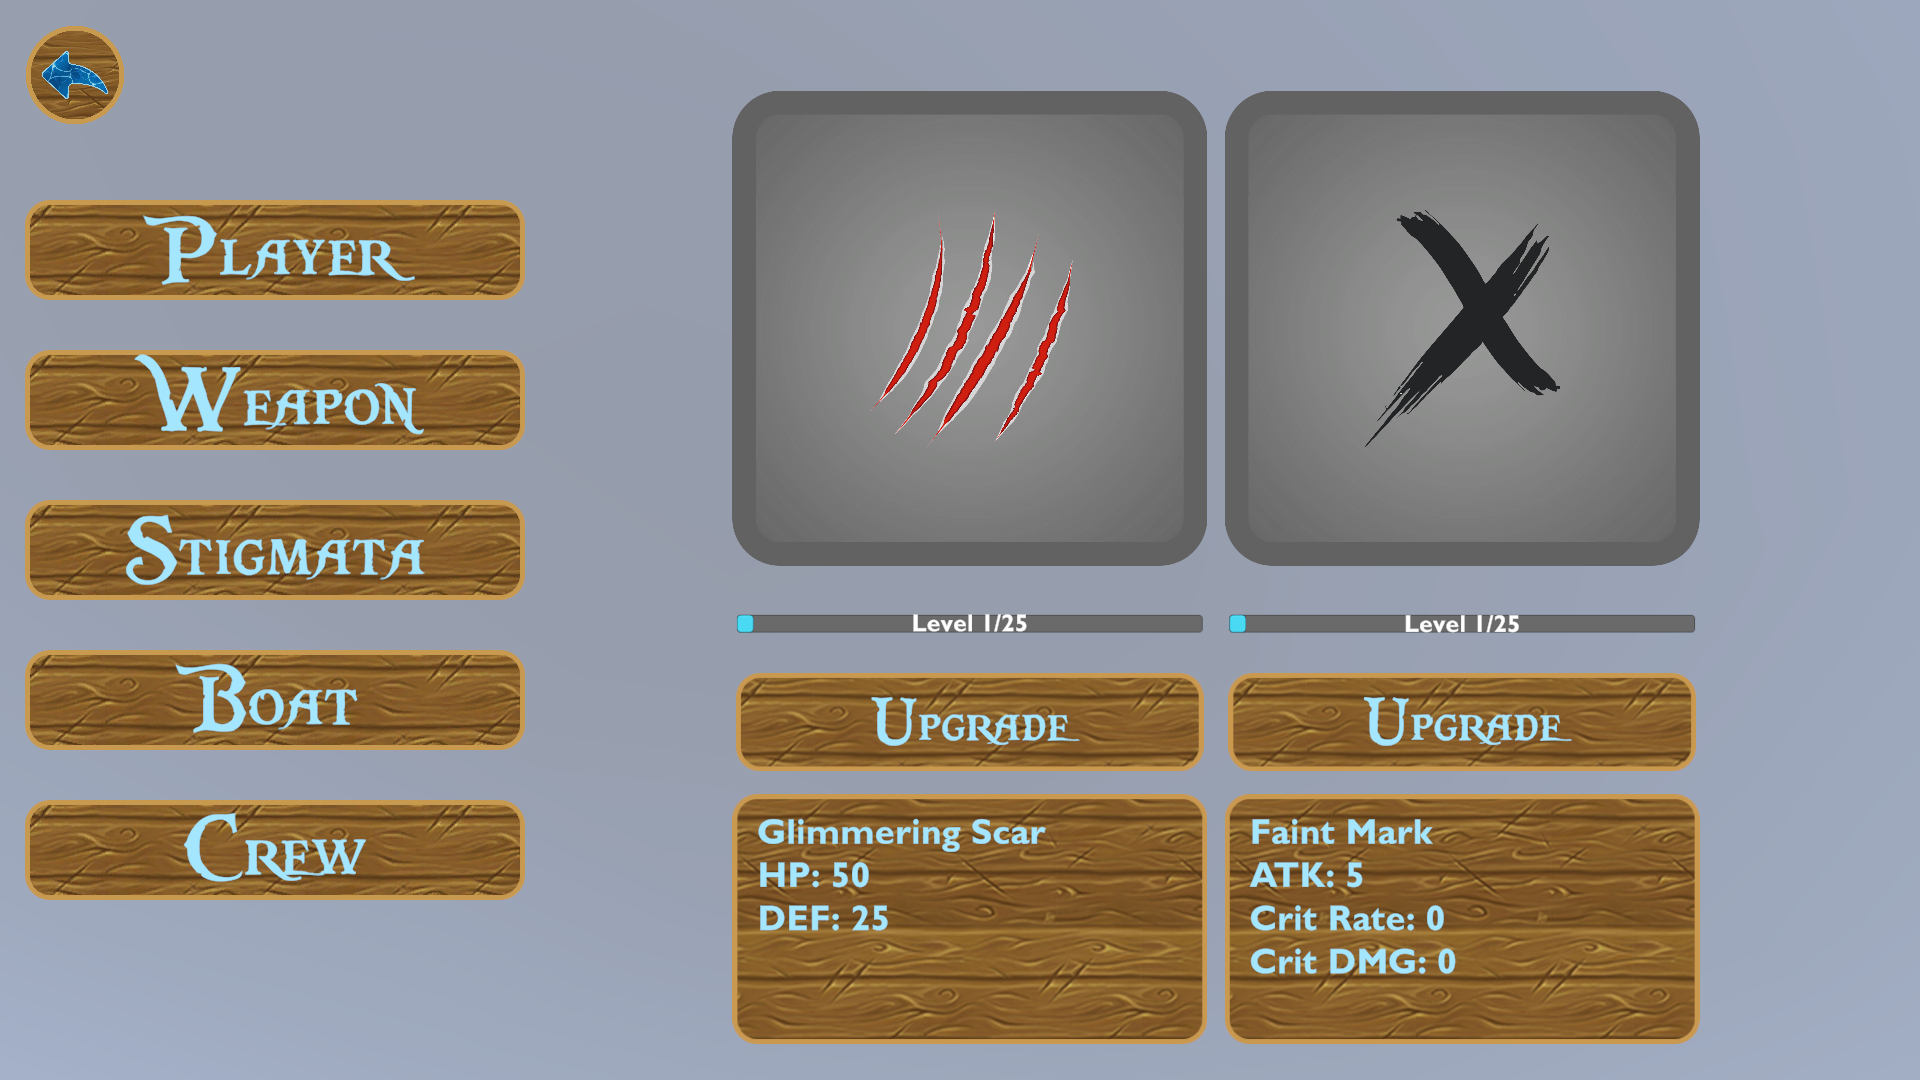
\includegraphics[width=5in]{Illustration/MenuUI/EquipmentMenu2.png}
\end{center}










\newpage
\subsection{Water Simulation}
\paragraph{Objectives}\hfill

One of the most important features of this project is the water simulation, which serves as the foundation for realistic water behavior and environmental interactions. Early in development, the focus was placed on creating wave and buoyancy systems that would allow floating objects to interact naturally with the water surface.

\paragraph{Implementation}\hfill

\noindent Initial Approach: Sine Wave Simulation

The initial implementation used a simple sine wave model. A WaveManager script calculated wave heights along the water's surface using a sine function based on the x-coordinate. These heights were applied to the vertices of the water mesh by the WaterManager script, dynamically updating the surface in real time.\\

A Floater script was created to simulate buoyancy, allowing objects like boats or debris to interact with waves by computing buoyant forces relative to the water height at their positions. This enabled vertical movement and tilting aligned with wave motion.\\

While effective for basic interaction, this method produced repetitive and mechanical wave patterns, lacking realism in large environments like oceans or lakes.\\

\noindent Transition to Gerstner Waves

To improve realism, the project transitioned to using Gerstner waves, based on research from CatLikeCoding.com. Unlike sine waves that affect only vertical displacement, Gerstner waves simulate both vertical and horizontal movement, mimicking the rolling behavior of real ocean waves.\\

Key parameters in the Gerstner wave model include:
\begin{itemize}
    \item Wave Direction (travel path of the wave)
    \item Wavelength (distance between wave peaks)
    \item Steepness (sharpness and intensity of waves)
    \item Speed (wave propagation rate)
\end{itemize}

The Gerstner formula computes vertex displacement by adjusting horizontal and vertical positions simultaneously, producing a more organic wave motion. Initially implemented with a single Gerstner wave, the system was later expanded to layer multiple waves with varying parameters to create complex, natural water behavior.

\begin{itemize}
    \item WaveManager: Updated to calculate combined horizontal and vertical displacements per vertex using layered Gerstner waves traveling in multiple directions.
    \item WaterManager: Modified to apply Gerstner wave displacements dynamically to the water mesh based on world coordinates.
    \item Floater: Adjusted to calculate buoyancy forces using Gerstner wave heights, enabling floating objects to respond realistically to rolling waves.
\end{itemize}

\begin{center}
    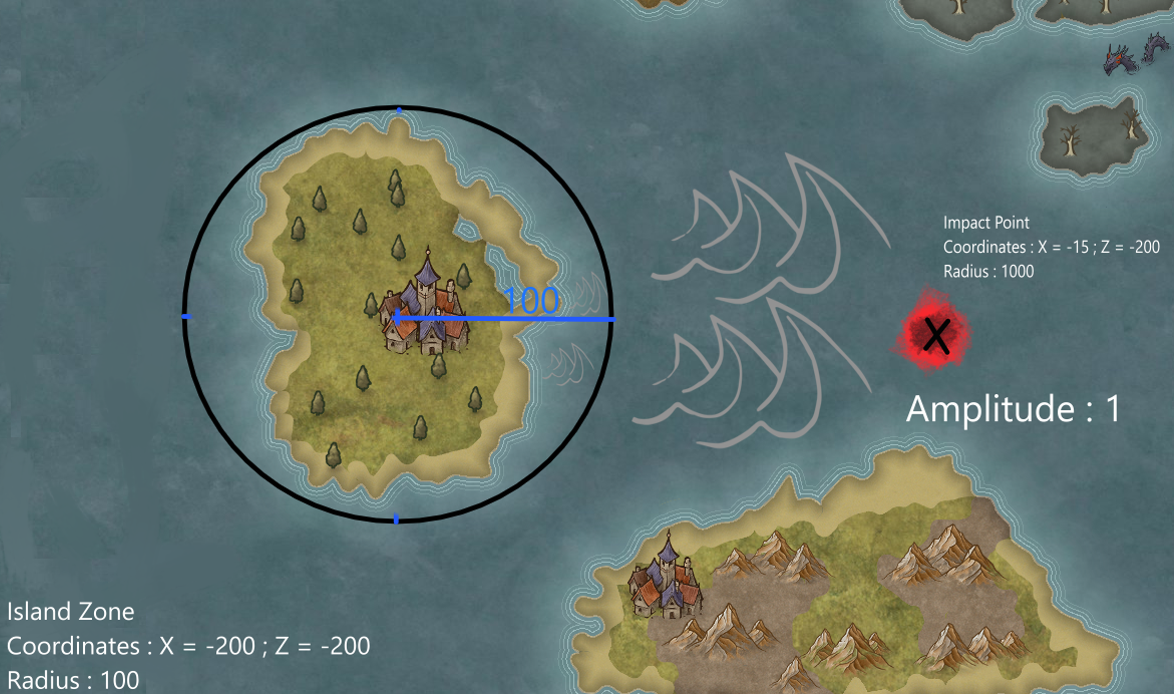
\includegraphics[width=5in]{Illustration/WaterSim/System_Eau.png}
\end{center}

\paragraph{Results}\hfill

The adoption of Gerstner waves significantly enhanced the water simulation:
\begin{itemize}
    \item Visual Realism: The rolling, dynamic motion greatly improved the water's authenticity and immersion.
    \item Customization: Adjustable parameters allow simulation of diverse water conditions, from calm lakes to stormy seas, supporting future climate simulation features.
    \item Complexity \& Flexibility: Layered waves moving in different directions create natural, unpredictable water surface behavior, enhancing gameplay interaction and environmental aesthetics.
\end{itemize}

This upgraded water simulation now provides a robust and adaptable foundation for further development, improving both the visual appeal and interactivity of the game environment.

\begin{center}
    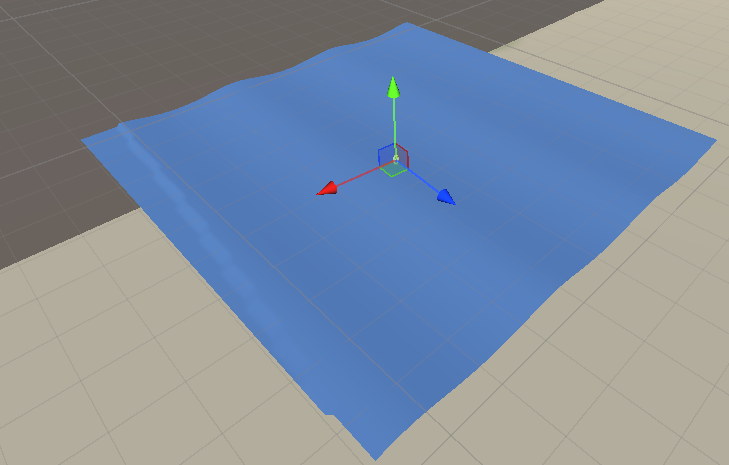
\includegraphics[width=5in]{Illustration/WaterSim/WaterSimulation.png}
\end{center}










\newpage
\subsection{Weather Simulation}
\paragraph{Objective}\hfill

The primary objective of this weather simulation project is to implement a dynamic rain effect within a Unity-based environment. The simulation is limited to rain, with the core requirement being the ability to initiate and stop rainfall at random time intervals. Additionally, performance optimization is a key consideration to ensure that the rain system does not negatively impact the overall gameplay experience. The rain should only appear within the player's vicinity rather than across the entire game world, thereby reducing unnecessary rendering and processing overhead.

\paragraph{Implementation}\hfill

The rain simulation was developed using Unity's built-in Particle System, following several online tutorials as initial references. One of the most important design choices was to constrain the rain effect to a localized area around the player rather than rendering it globally across the map. This approach greatly improves performance by limiting the number of active particles and focusing computational resources only where necessary.\\

The implementation process began by configuring a basic rain effect using Unity's Particle System. This part of the development was relatively straightforward and involved tuning the particle settings to visually represent rainfall convincingly. However, a static and always-on rain system would not meet the design requirements. Therefore, a custom script was developed to control the activation and deactivation of the rain effect.\\

The script triggers the rain effect at random intervals and allows it to run for a fixed duration—currently set to three minutes—before deactivating it. These time-based triggers help in creating a more dynamic and realistic weather pattern within the game environment. Activating and deactivating the Particle System in Unity was achieved through a simple scripting interface, making the implementation efficient and lightweight.\\

To ensure that the rain follows the player regardless of movement, the Particle System was parented to the player's prefab. This ensures that the rain zone—implemented as a cylindrical volume around the player—moves with the player character seamlessly. By doing this, we simulate a localized weather effect that maintains immersion without causing a significant drop in performance.

\paragraph{Results}\hfill

The final implementation of the rain simulation met the project's goals. The rain starts at randomized intervals and lasts for a predetermined period of three minutes. By generating particles within a cylindrical area centered around the player, the system avoids rendering unnecessary particles elsewhere in the game world. This localized particle emission strategy significantly enhances performance efficiency, especially important when the weather system is a secondary feature in a more complex game environment.

\begin{center}
    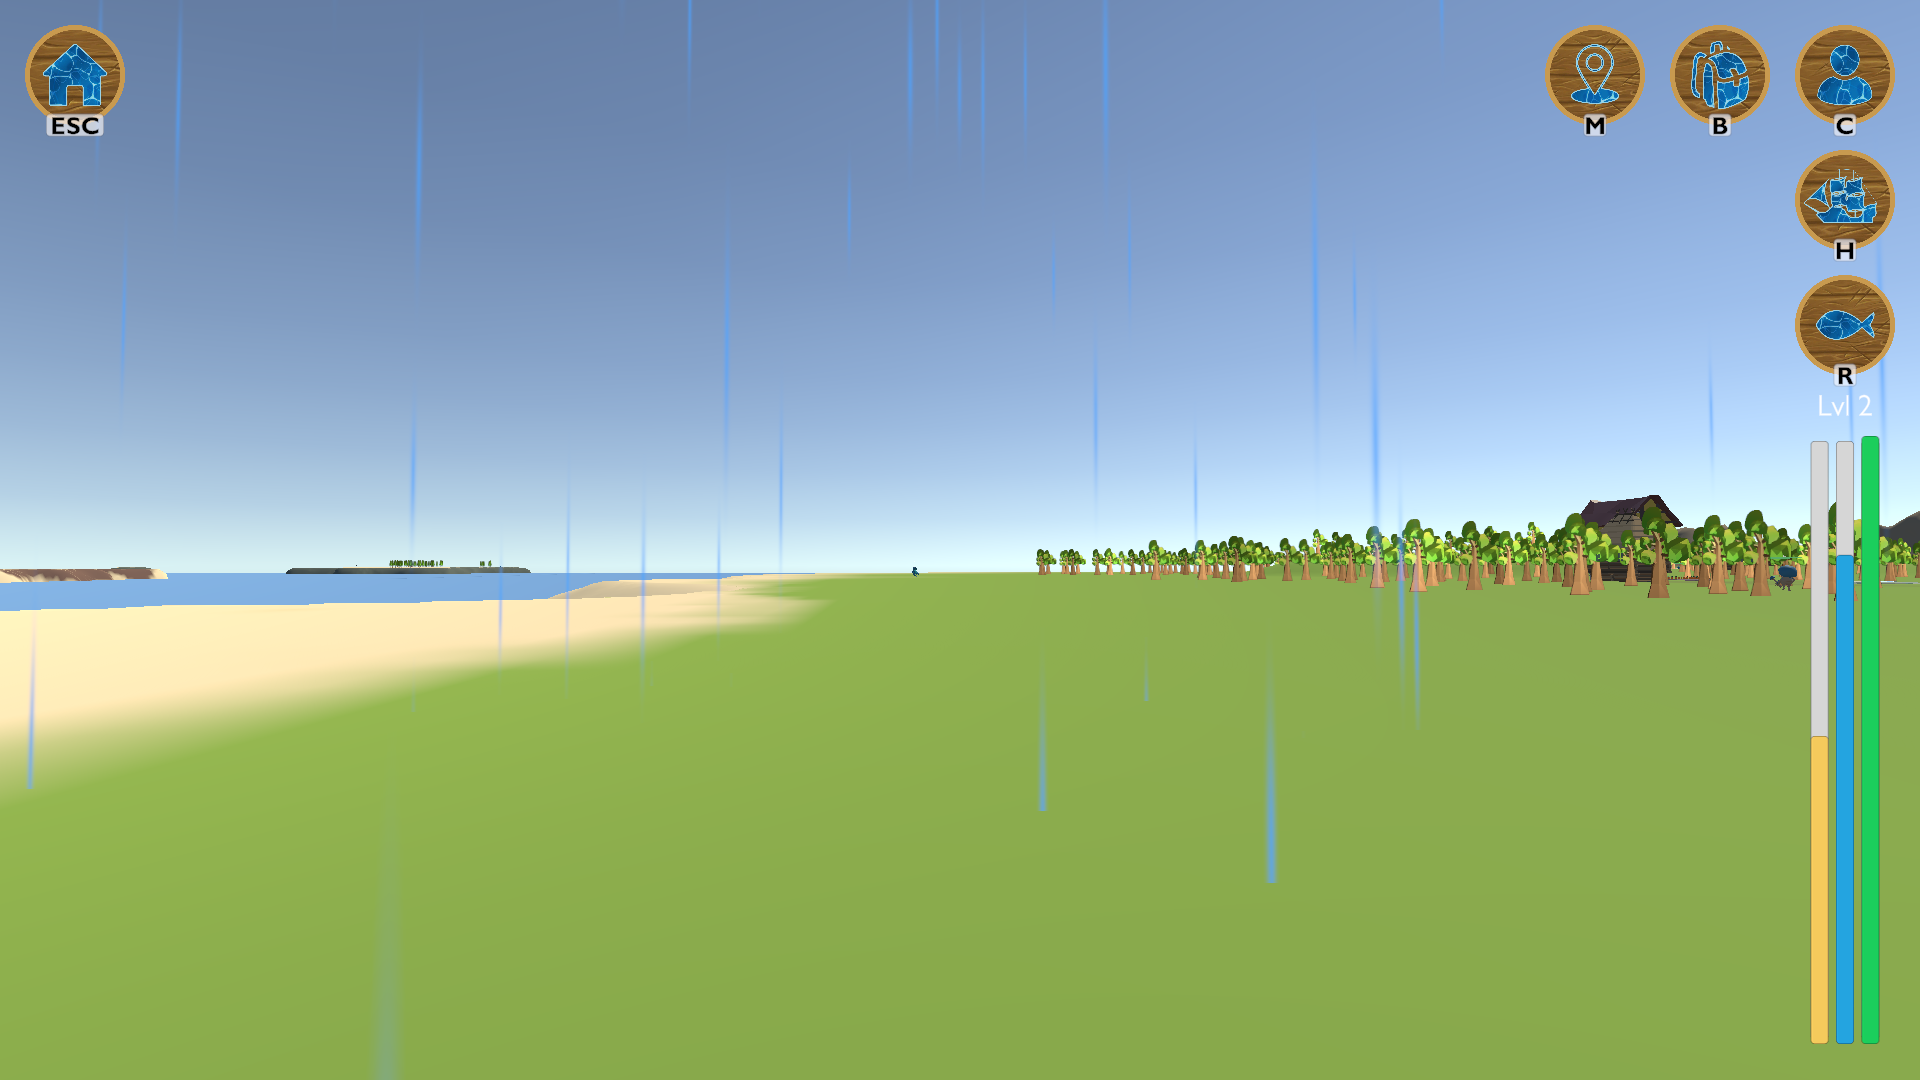
\includegraphics[width=5in]{Illustration/Weather/Rain.png}
\end{center}


Overall, the system provides a simple yet effective weather simulation that balances visual realism with performance optimization.










\newpage
\subsection{Player Movement}
\paragraph{Objectives}\hfill

A core component of the gameplay experience in an open-world environment is the implementation of fluid and responsive player movement. Movement must be intuitive, immersive, and enjoyable, as it serves as the foundation of user interaction within the game world. The goal was to develop a system that would handle walking, jumping, and camera control smoothly across varied terrain, ensuring an engaging and seamless exploration experience.

\paragraph{Implementation}

Research and experimentation identified two main approaches for player movement in Unity: using a Character Controller or a Rigidbody. After comparing both methods, the Character Controller was chosen due to its better handling of complex terrains such as slopes, stairs, and uneven ground, which are prevalent in the game's rugged open-world environment.\\

An object was created to represent the player, and although a Rigidbody component was initially tested, the final system used only the Character Controller.\\

A custom movement script was developed to define key constants such as:
\begin{itemize}
    \item Gravity
    \item Movement speed
    \item Jump height
\end{itemize}

Unity's Input class was used to capture keyboard input. A 3D movement vector was calculated based on the player's directional inputs, scaled by the movement speed, and applied to the Character Controller to move the player smoothly in the intended direction.\\

To simulate gravity, a constant downward force was applied to the player, allowing for realistic falling and grounded movement. The system continuously checks whether the player is grounded to apply gravity appropriately.\\

Jumping functionality was also implemented using the Input class to detect the jump key. When the player is grounded and the jump input is triggered, a vertical force is applied, calculated based on the jump height and gravity values. This prevents mid-air jumping and ensures physically accurate movement.\\

For improved immersion, a mouse-based camera control system was developed. Mouse movement is captured through the Input class and applied to the player's camera, enabling smooth horizontal and vertical rotation. This allows players to freely look around in both first-person and third-person views.

\paragraph{Results}\hfill

The final movement system provided smooth and responsive navigation, realistic gravity behavior, and an accurate jumping mechanic. The use of Unity's Character Controller proved effective for managing movement across a variety of terrains, contributing to an enjoyable and reliable player experience.\\

Additionally, the implementation of mouse-based camera control enhanced immersion, allowing players to engage more naturally with their surroundings. This movement system forms a robust foundation for exploration and interaction within the open-world environment, supporting further gameplay features and contributing to overall user satisfaction.










\newpage
\subsection{Boat Simulation}
\paragraph{Objective}\hfill

The goal of the boat simulation was to deliver a fluid and immersive sailing experience within the game, one that captured the physicality and responsiveness of navigating a vessel in a dynamic environment. Unlike the player movement, which relied on Unity's Character Controller for handling interactions with uneven terrain, the boat required a more physically accurate simulation. The aim was to leverage Unity's Rigidbody system to replicate the forces acting on a real ship, from steering and propulsion to anchoring and wind-based navigation. Additionally, intuitive and interactive ship controls—such as a helm and capstan—were necessary to give players a meaningful and engaging way to operate the vessel.

\paragraph{Implementation}\hfill

To achieve realistic movement, the ship was modeled using Unity's Rigidbody component, allowing it to respond naturally to applied forces and torque. This physics-based approach enabled the boat to exhibit weight and momentum, which are essential for authentic sailing dynamics. Unlike character movement, where directional input can be applied directly, the ship's control required handling inertia and resistance more carefully.\\

The core of the ship's behavior was governed by two primary functions. The first, responsible for rotation, was triggered when a player interacted with the helm. It captured mouse input to determine steering direction and applied rotational torque to the Rigidbody, allowing smooth and responsive turning. The second function handled forward movement, applying velocity along the ship's local Z-axis. To simulate realistic anchoring behavior, this function included a check to disable propulsion when the anchor was deployed.\\

Interactivity was managed through a ray casting system. When the player looked at the helm or capstan and pressed a designated key, a ray was projected from the camera. If the ray collided with the appropriate object, such as the capstan's collider, the related interaction—like raising or lowering the anchor—was triggered. This same approach was used for helm control, offering a consistent and user-friendly way to manage various ship components.\\

\begin{center}
    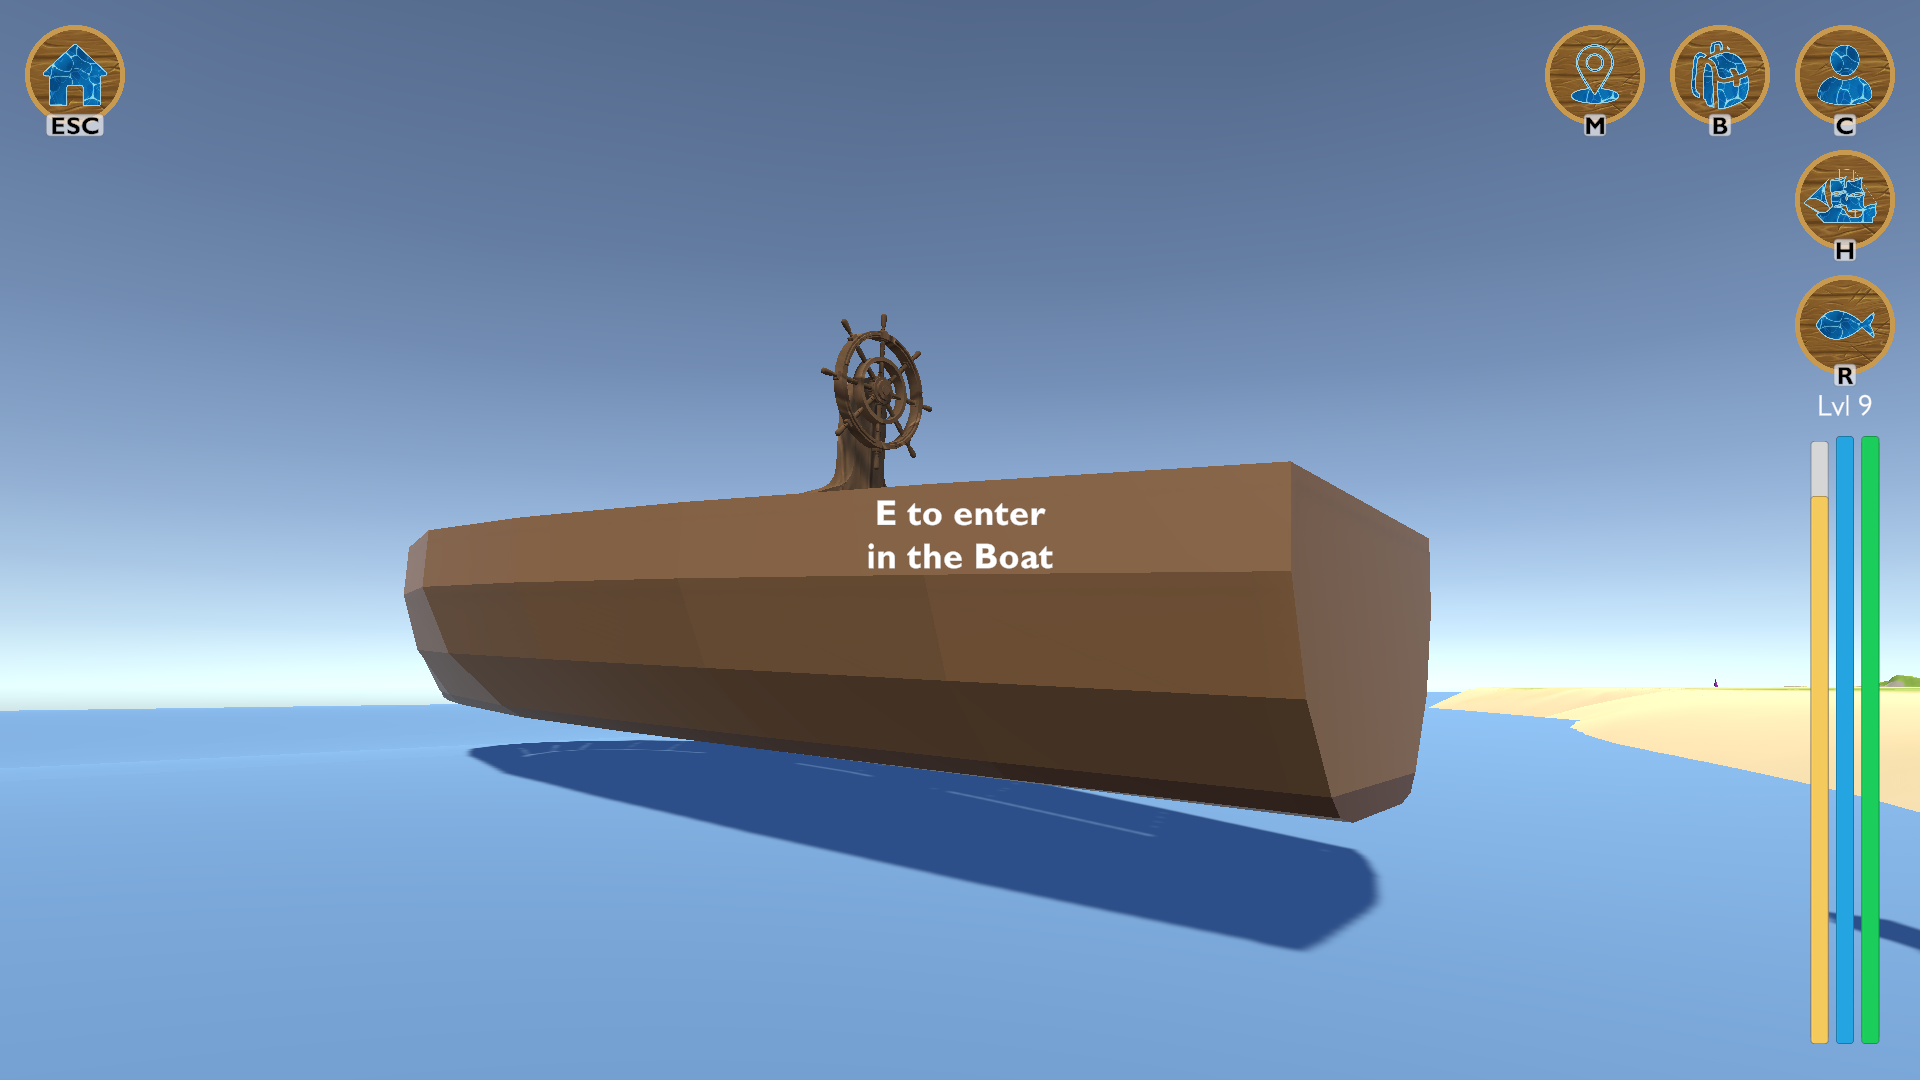
\includegraphics[width=5in]{Illustration/BoatMovement/EnterBoat.png}
    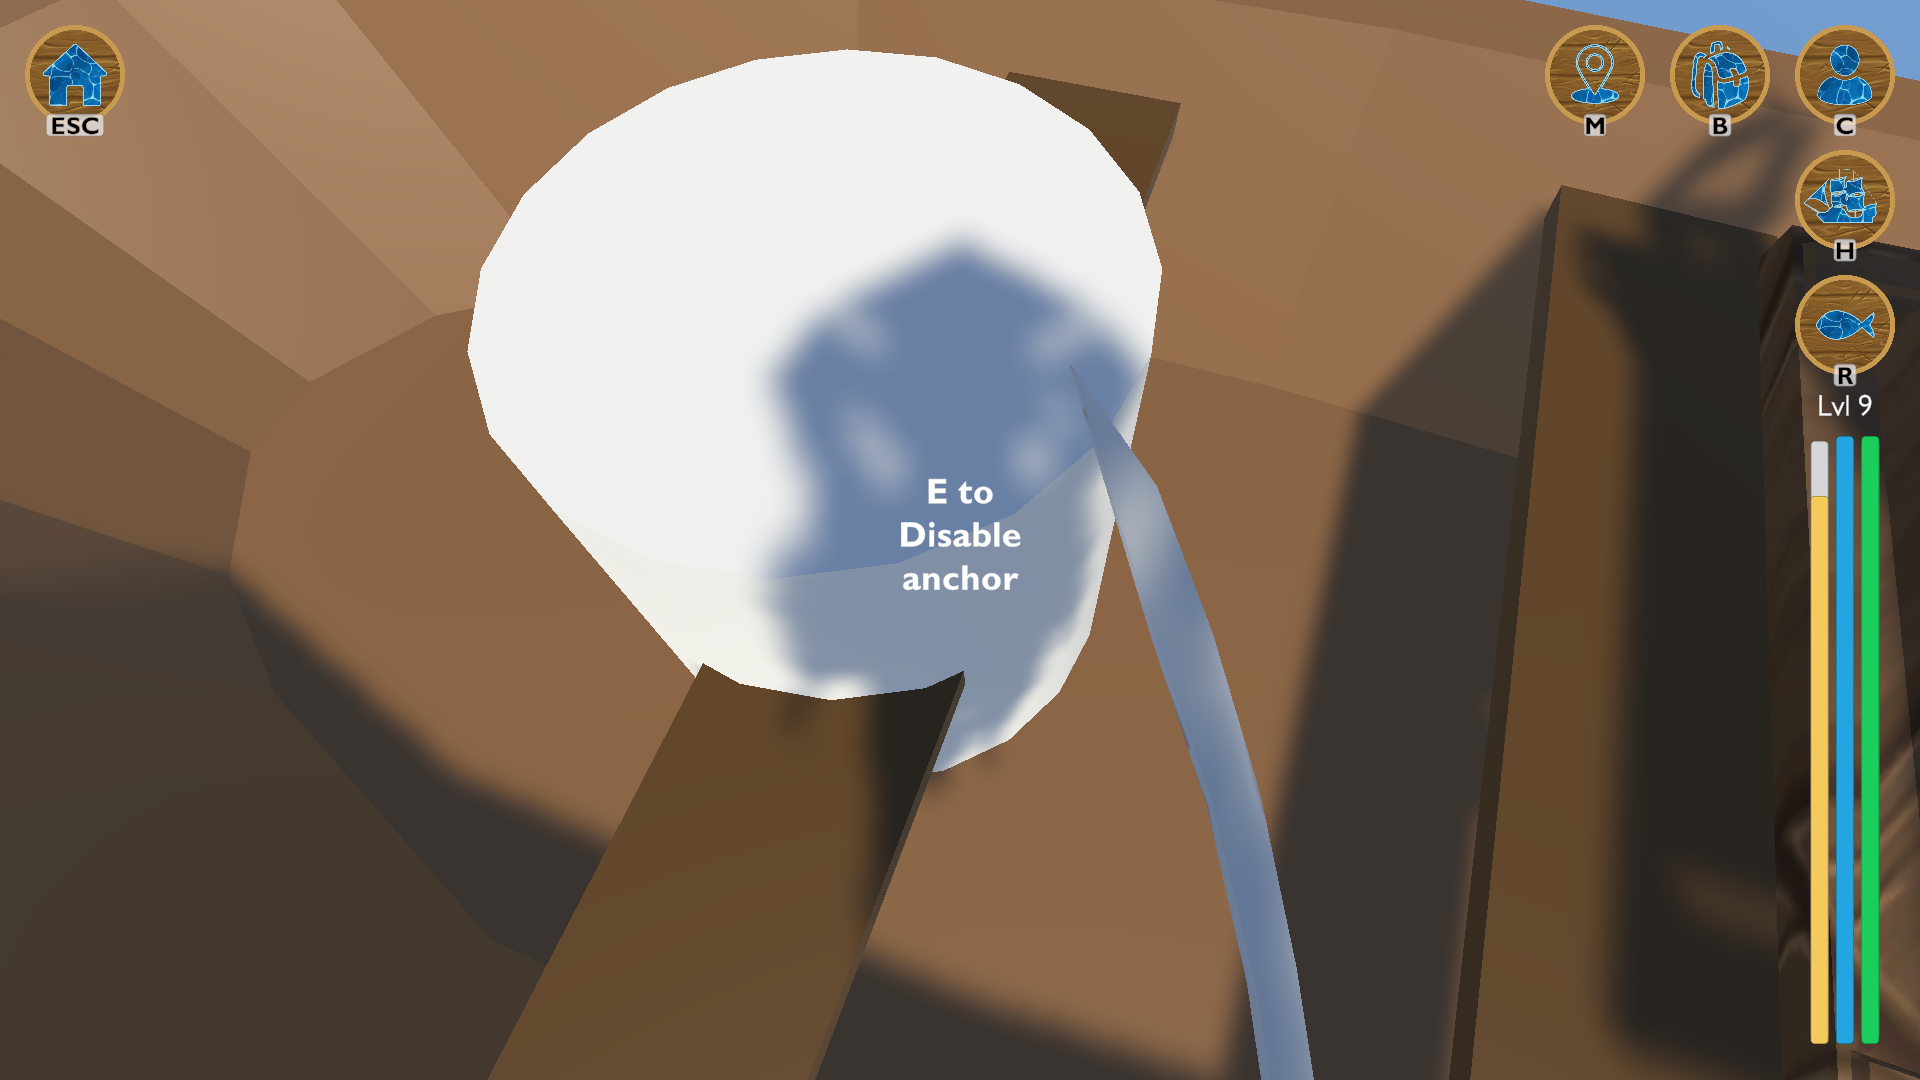
\includegraphics[width=5in]{Illustration/BoatMovement/Anchor.png}
    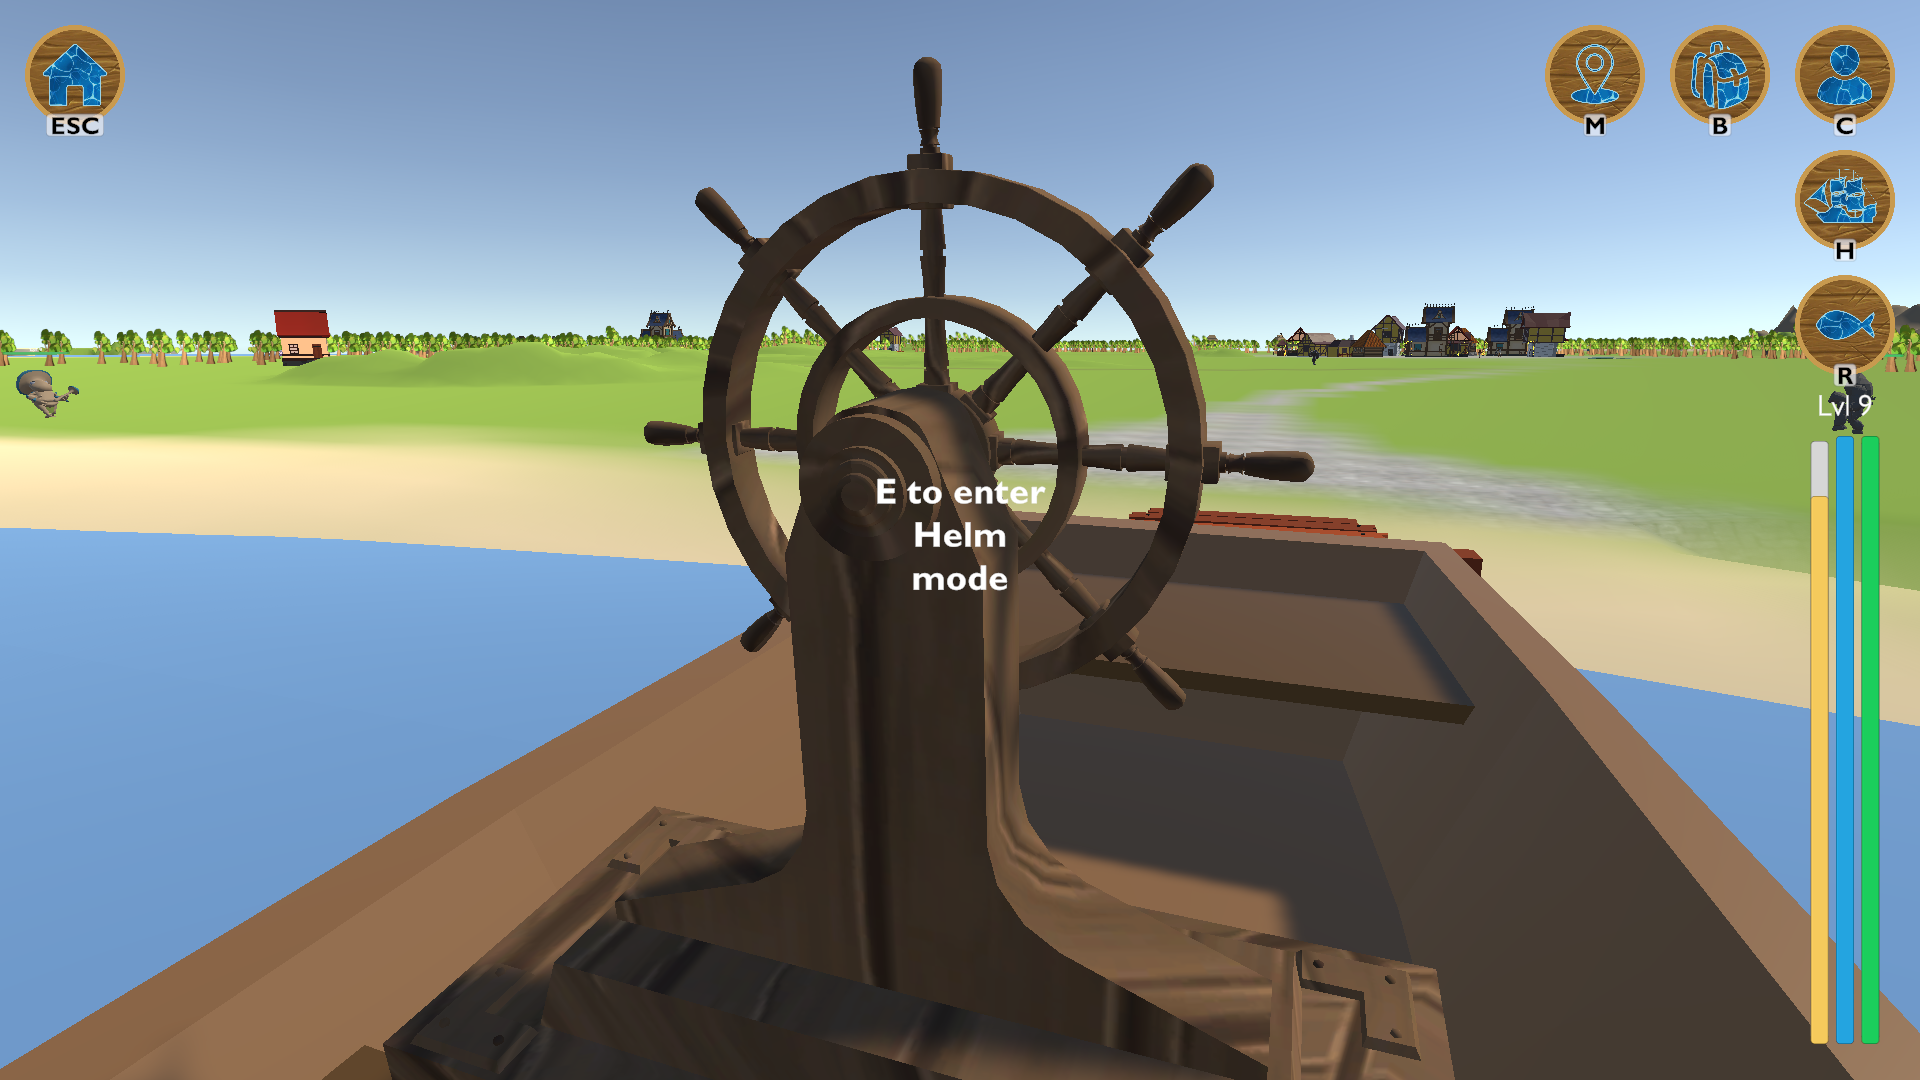
\includegraphics[width=5in]{Illustration/BoatMovement/Helm.png}
\end{center}

Development drew heavily on online resources. A Unity tutorial on Rigidbody-based movement and player interaction (\url{https://youtu.be/_QajrabyTJc}) was instrumental in implementing the basic control structure. Sailing mechanics were informed by a video explaining wind and trigonometry in game development (\url{https://youtu.be/_zDF40XFWN4}). In addition, real-world sailing principles—specifically the optimal sail-to-wind angle of approximately 38°—were referenced from research conducted at the University of Miami's Rosenstiel School of Marine and Atmospheric Science. This figure informed the wind-based movement logic and helped fine-tune the responsiveness of the ship to its environment.\\

Key constants were defined for movement speed, helm rotation, and wind interaction, all of which contributed to a responsive and engaging sailing experience.

\paragraph{Result}\hfill

The finished boat simulation succeeded in delivering a responsive and believable sailing system. The use of Rigidbody physics gave the ship convincing weight and momentum, making movement feel more grounded and satisfying. Steering through mouse input and torque created a smooth navigation experience, while forward propulsion responded appropriately to anchor states and wind conditions.\\

The integration of ray casting for player interaction allowed for intuitive control over key ship elements, and the anchor system functioned reliably as part of this broader interaction model. Together, these elements created a cohesive and immersive sailing mechanic that significantly elevated the maritime aspects of gameplay.\\

Most importantly, the system is built with future scalability in mind. The wind and control logic can be expanded further to include more advanced weather systems or AI ship navigation.










\newpage
\subsection{AI}
\paragraph{Objective}\hfill

The primary objective of the artificial intelligence (AI) development process was to address a series of persistent issues affecting the behavior of non-playable characters (NPCs) and enemy units within the game environment. These issues included unpredictable movement patterns, unreliable detection of player proximity, and failure to initiate or sustain interactions effectively. Such inconsistencies disrupted the immersive quality of the game world and had a detrimental impact on both narrative progression and gameplay fluidity.\\

To resolve these challenges, the aim was to implement a robust and scalable AI system that delivered realistic character behavior, smooth and intelligent navigation, and coherent interaction logic. This new system would need to enable NPCs and enemies to react appropriately to dynamic changes in the game environment, support diverse behaviors such as patrolling or pursuing, and provide a solid foundation for future gameplay systems including combat, dialogue, and quest triggers.\\

A secondary objective involved the exploration and effective implementation of Unity's NavMesh (Navigation Mesh) system, which facilitates AI navigation by generating walkable areas on the game terrain. Mastery of this tool was essential to ensuring controlled, efficient, and believable movement across the environment.

\paragraph{Implementation}\hfill

The process began with a comprehensive debugging and diagnostic phase. Early AI prototypes displayed erratic movement behaviors, such as enemies clipping through objects, overshooting destinations, or failing to engage with the player under expected conditions. These anomalies suggested deeper issues within the navigation logic and interaction framework.\\

Each behavior was examined through isolated test scenarios that simulated real gameplay conditions. These included enemy approaches from different angles, NPC responses in varying terrain configurations, and obstacle-dense environments. The aim was to understand under what conditions the existing AI systems failed and to identify specific causes such as improper collider setups, missing NavMesh data, or poorly configured agent parameters.\\

Unity's NavMesh debugger and visual overlay tools were extensively used to inspect navigation paths, agent boundaries, and unreachable zones. These tools revealed that in many cases, the navigation mesh did not accurately reflect the intended walkable surfaces, leading to failed pathfinding attempts or invalid agent states.\\

\begin{center}
    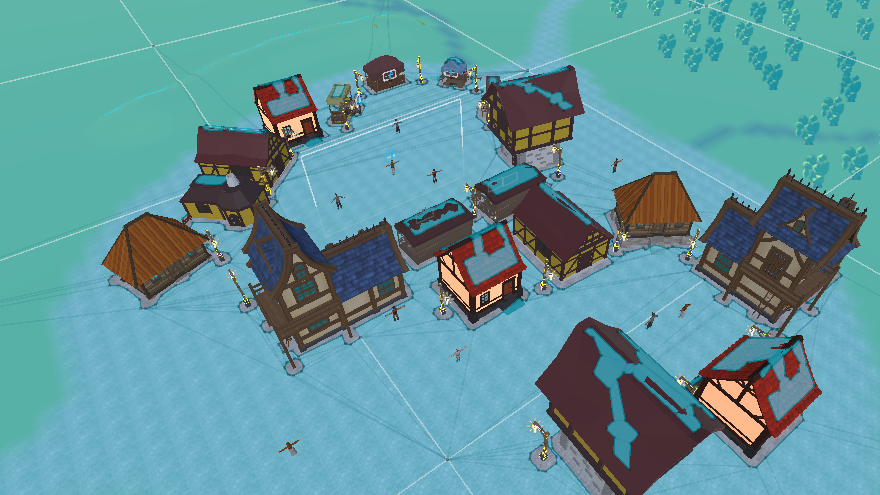
\includegraphics[width=5in]{Illustration/AI/NavMesh1.png}
    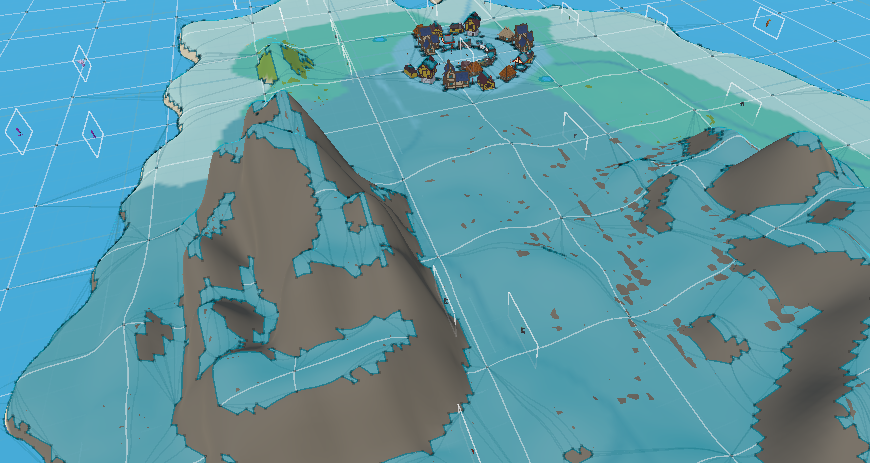
\includegraphics[width=5in]{Illustration/AI/NavMesh2.png}
\end{center}

To address the navigation issues, focused efforts were placed on learning and implementing the NavMesh system. Tutorials, documentation, and hands-on testing provided a solid understanding of how to bake navigation data, place NavMesh obstacles, and configure navigation agents with customized behaviors.\\

Once a base understanding was established, the first test scene was created using a simplified environment. A NavMesh surface component was added to the terrain, and navigation baking was performed to generate a walkable mesh. AI agents (representing NPCs) were configured with NavMeshAgent components and a custom movement script. This setup allowed the AI to wander within a specified radius using randomized destinations within the navigable area.\\

The basic wandering behavior was extended by implementing additional state logic, enabling agents to transition between idle, patrol, and interaction states. The patrol state used waypoints, while the idle state incorporated timed pauses and turning animations to simulate more lifelike behavior.\\

A subsequent version of the AI system introduced aggressive behavior patterns. Enemies were programmed to detect the player's presence using trigger colliders or raycasting, then transition to a pursuit state. However, early iterations exhibited a critical flaw: enemies would move directly to the player's exact position, continuously pushing into them and disrupting gameplay flow.\\

\begin{center}
    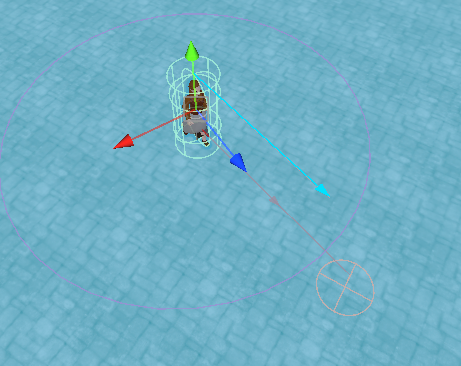
\includegraphics[width=3in]{Illustration/AI/Passiv.png}
    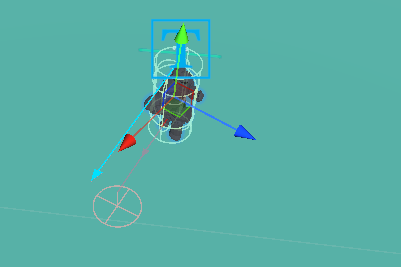
\includegraphics[width=3in]{Illustration/AI/Offensiv.png}
\end{center}

To resolve this, custom logic was written to measure the distance between the AI agent and the player in real-time. When within a predefined stopping distance, the agent would halt and orient itself toward the player without making further movement requests. This preserved proximity-based combat without the collision issues seen in earlier builds.\\

Fine-tuning the NavMeshAgent parameters was essential here. The following adjustments were made:
\begin{itemize}
    \item Stopping Distance was increased to prevent crowding the player.
    \item Acceleration and Angular Speed were lowered to create more deliberate, readable enemy movements.
    \item Auto-Braking was enabled to ensure smoother deceleration as agents approached their targets.
\end{itemize}

Additional behavior trees and finite state machines (FSMs) were implemented to govern enemy responses. These included logic for:
\begin{itemize}
    \item Returning to a patrol route if the player escaped.
    \item Entering an alert state upon detection of nearby sounds or events.
    \item Coordinating attack animations once within striking distance.
\end{itemize}

\paragraph{Result}\hfill

The implementation and refinement of the AI system significantly enhanced the overall quality of gameplay. Through the use of Unity's NavMesh system and the development of tailored behavior scripts, both enemies and NPCs now move intelligently and behave contextually in response to player actions and environmental stimuli.\\

Enemy units engage the player with more tactical awareness, maintain appropriate distance during combat, and navigate around obstacles efficiently. NPCs contribute to a more immersive world by exhibiting natural movement patterns and lifelike reactions, reinforcing the narrative atmosphere of the game.\\

These improvements have resulted in:
\begin{itemize}
    \item Stable and responsive AI behavior across varied gameplay scenarios.
    \item Realistic interactions between the player and game entities.    
\end{itemize}

The successful deployment of the new AI system has laid a strong foundation, ensuring that the artificial intelligence in the game remains dynamic and deeply integrated into the core gameplay experience.










\newpage
\subsection{Combat System}
\paragraph{Objective}\hfill

The primary goal was to enhance the combat mechanics by introducing an attack cooldown system, improving player feedback through visual indicators, and integrating contextual enemy animations. This was aimed at preventing repetitive attack spamming, promoting fair combat pacing, and delivering a more immersive and strategic gameplay experience.

\paragraph{Implementation}\hfill

The foundational combat system was already in place, with key variables such as player and enemy attack damage, as well as enemy health, being accurately tracked. The first enhancement was the implementation of an attack cooldown interval using Unity's built-in timing functions. This effectively limited how frequently the player could attack, creating a more balanced and engaging flow during encounters.\\

To improve real-time feedback, an enemy health bar was added using Unity's Slider component within the Canvas system. This visual indicator allowed players to track enemy health during combat, aiding tactical decision-making.\\

Additionally, a damage display system was implemented using TextMeshPro. When the player dealt damage, a floating number briefly appeared above the enemy to show the exact damage value, reinforcing the impact of attacks and enhancing combat clarity.\\

\begin{center}
    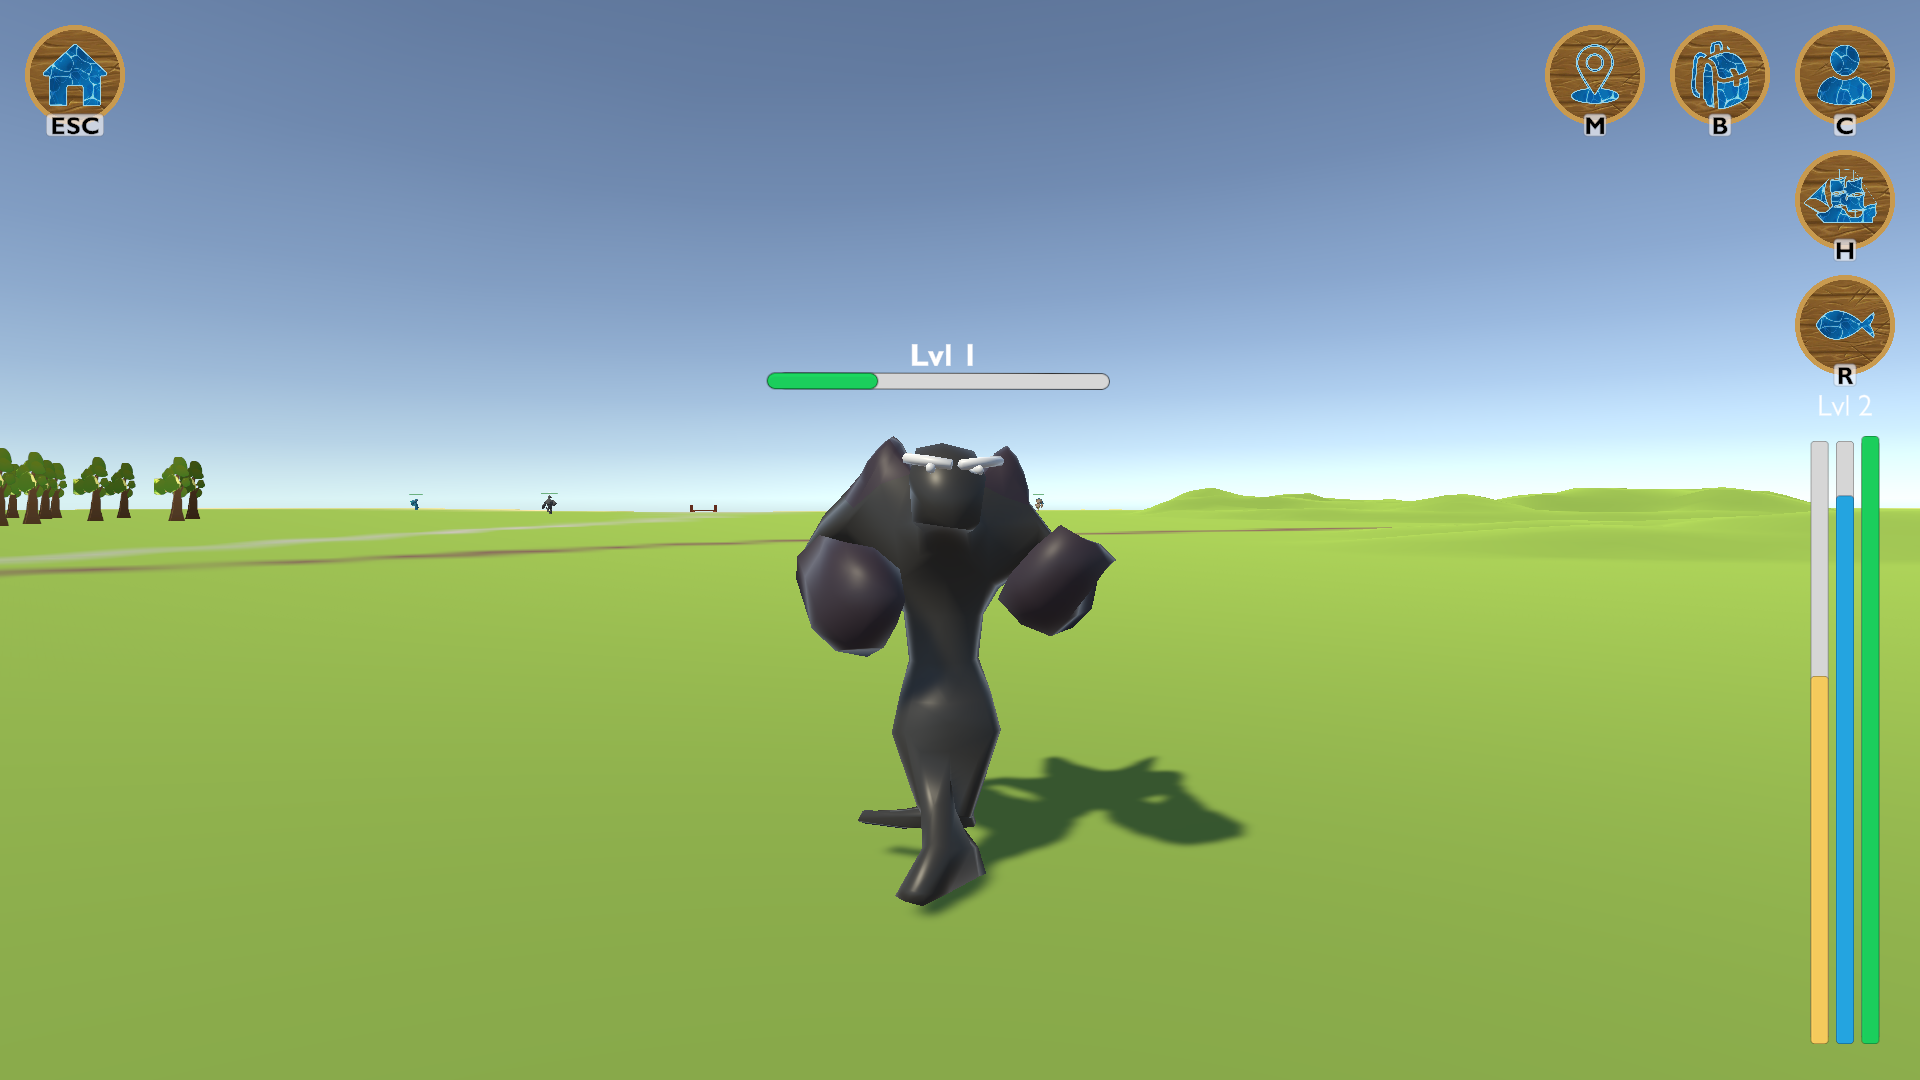
\includegraphics[width=3in]{Illustration/Combat/TerestrialEnemy.png}
    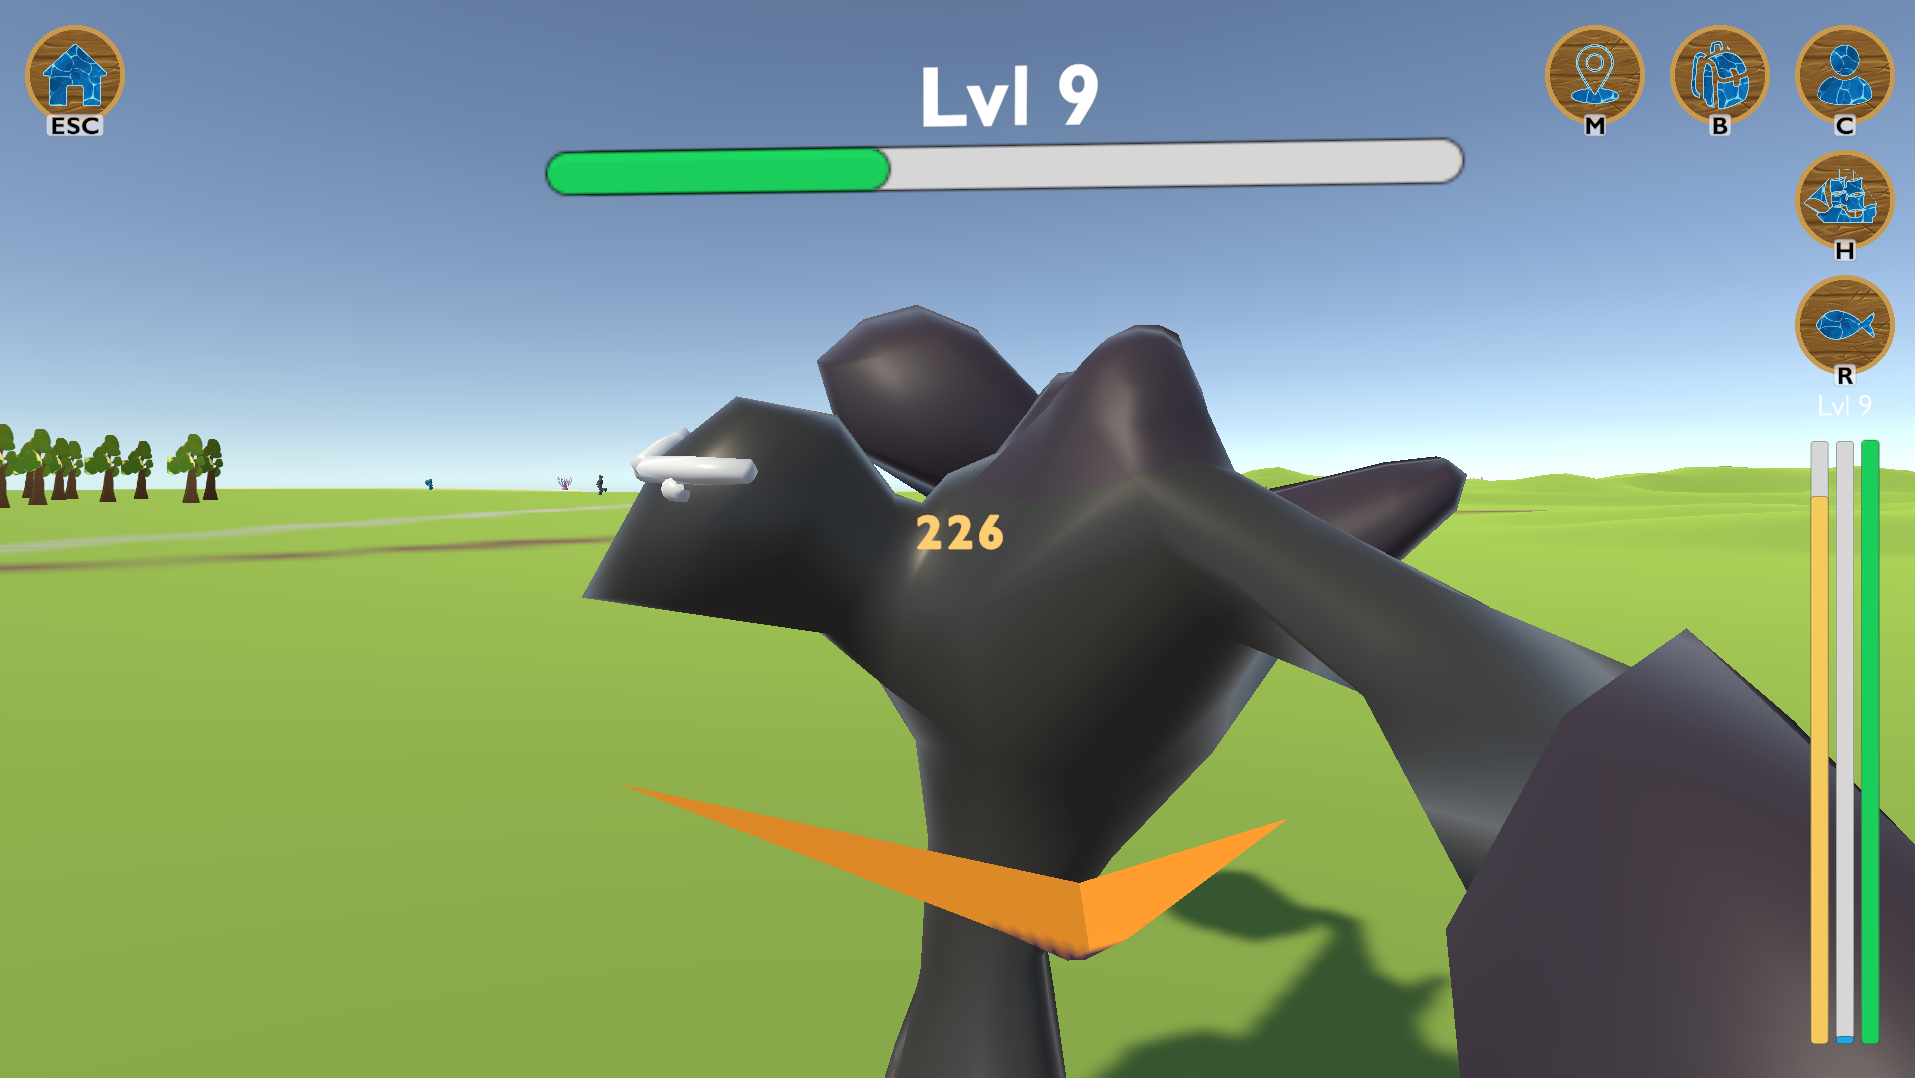
\includegraphics[width=5in]{Illustration/Combat/CombatTerestrial.png}
\end{center}

Enemy animations were created and managed through Unity's Animator Controller. Animations included idle, running, attacking, and death, and were triggered based on the enemy's behavior and current state. Since the player animation system was already developed, the enemy animation integration was efficient and consistent.\\

For maritime enemies, a simplified behavior model was implemented. These enemies had custom stats and were designed to attack the player's boat instead of the player directly. They remained stationary, had no animations, and triggered damage when in close proximity. Upon the boat's destruction (i.e., when its health reached zero), both the boat and the player were removed from the scene, simulating a game-over condition at sea.

\begin{center}
    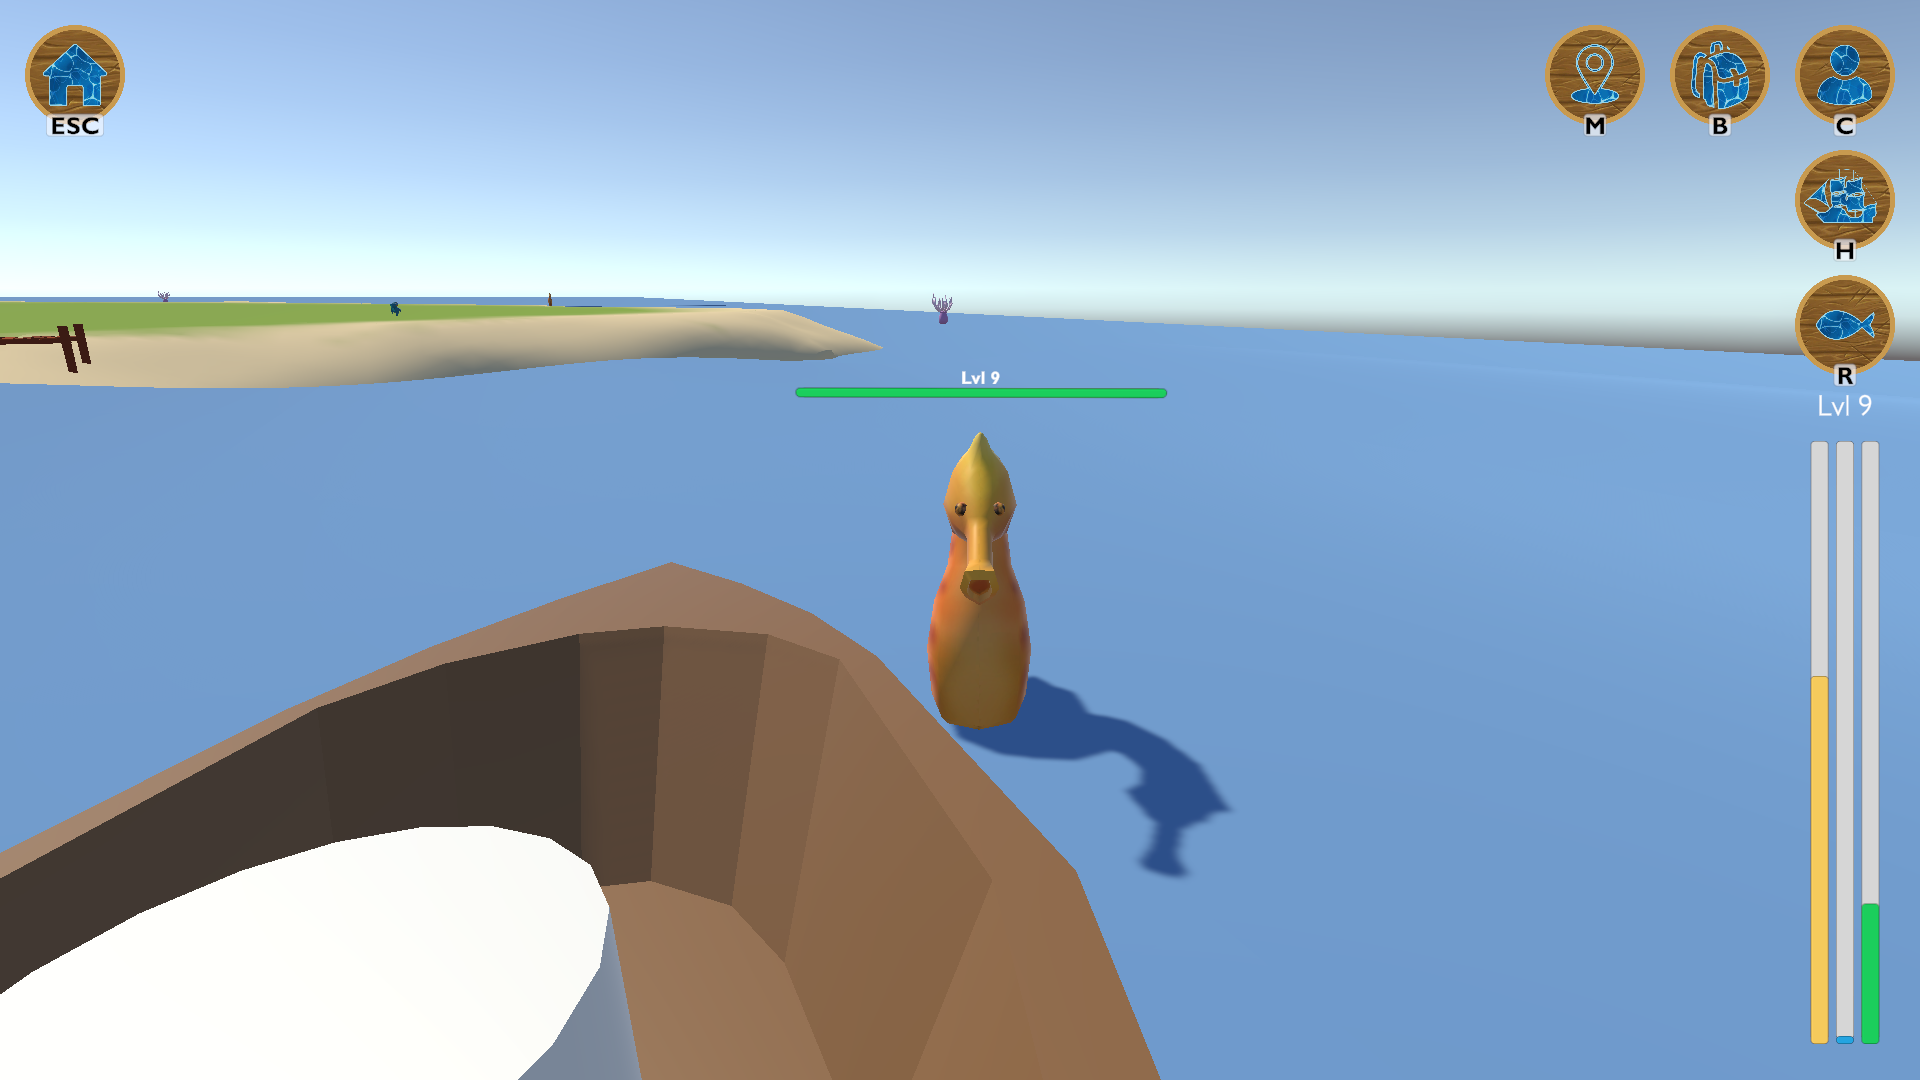
\includegraphics[width=5in]{Illustration/Combat/CombatMaritim.png}
\end{center}

\paragraph{Result}\hfill

The finalized attack system successfully improved the overall combat experience. The introduction of an attack cooldown encouraged more strategic timing and prevented exploitative button mashing. The combination of health bars and floating damage indicators delivered clear and immediate feedback, enhancing situational awareness for players.\\

The addition of responsive and context-appropriate enemy animations contributed to a more dynamic and visually satisfying combat flow. Meanwhile, the unique implementation for maritime enemies introduced variety and expanded gameplay mechanics without overcomplicating design.\\

These refinements laid a solid foundation for more advanced combat systems in future updates, while significantly elevating the current quality and polish of gameplay.











\newpage
\subsection{Map}
\paragraph{Objective}\hfill

The primary objective was to transform the original 2D map, created in the early stages of development, into a fully realized 3D environment using Unity's terrain system. The map features eight distinct islands, each with unique layouts and characteristics that needed to be faithfully recreated in 3D to maintain consistency with the initial design vision.

\paragraph{Implementation}\hfill

The process began by carefully shaping each island to match the outlines of the 2D map. Terrain heights were initially set to a base level to capture the general form and silhouette of each island. Following this, the terrain was smoothed to eliminate harsh elevation changes, ensuring natural slopes and realistic geographical features.\\

\begin{center}
    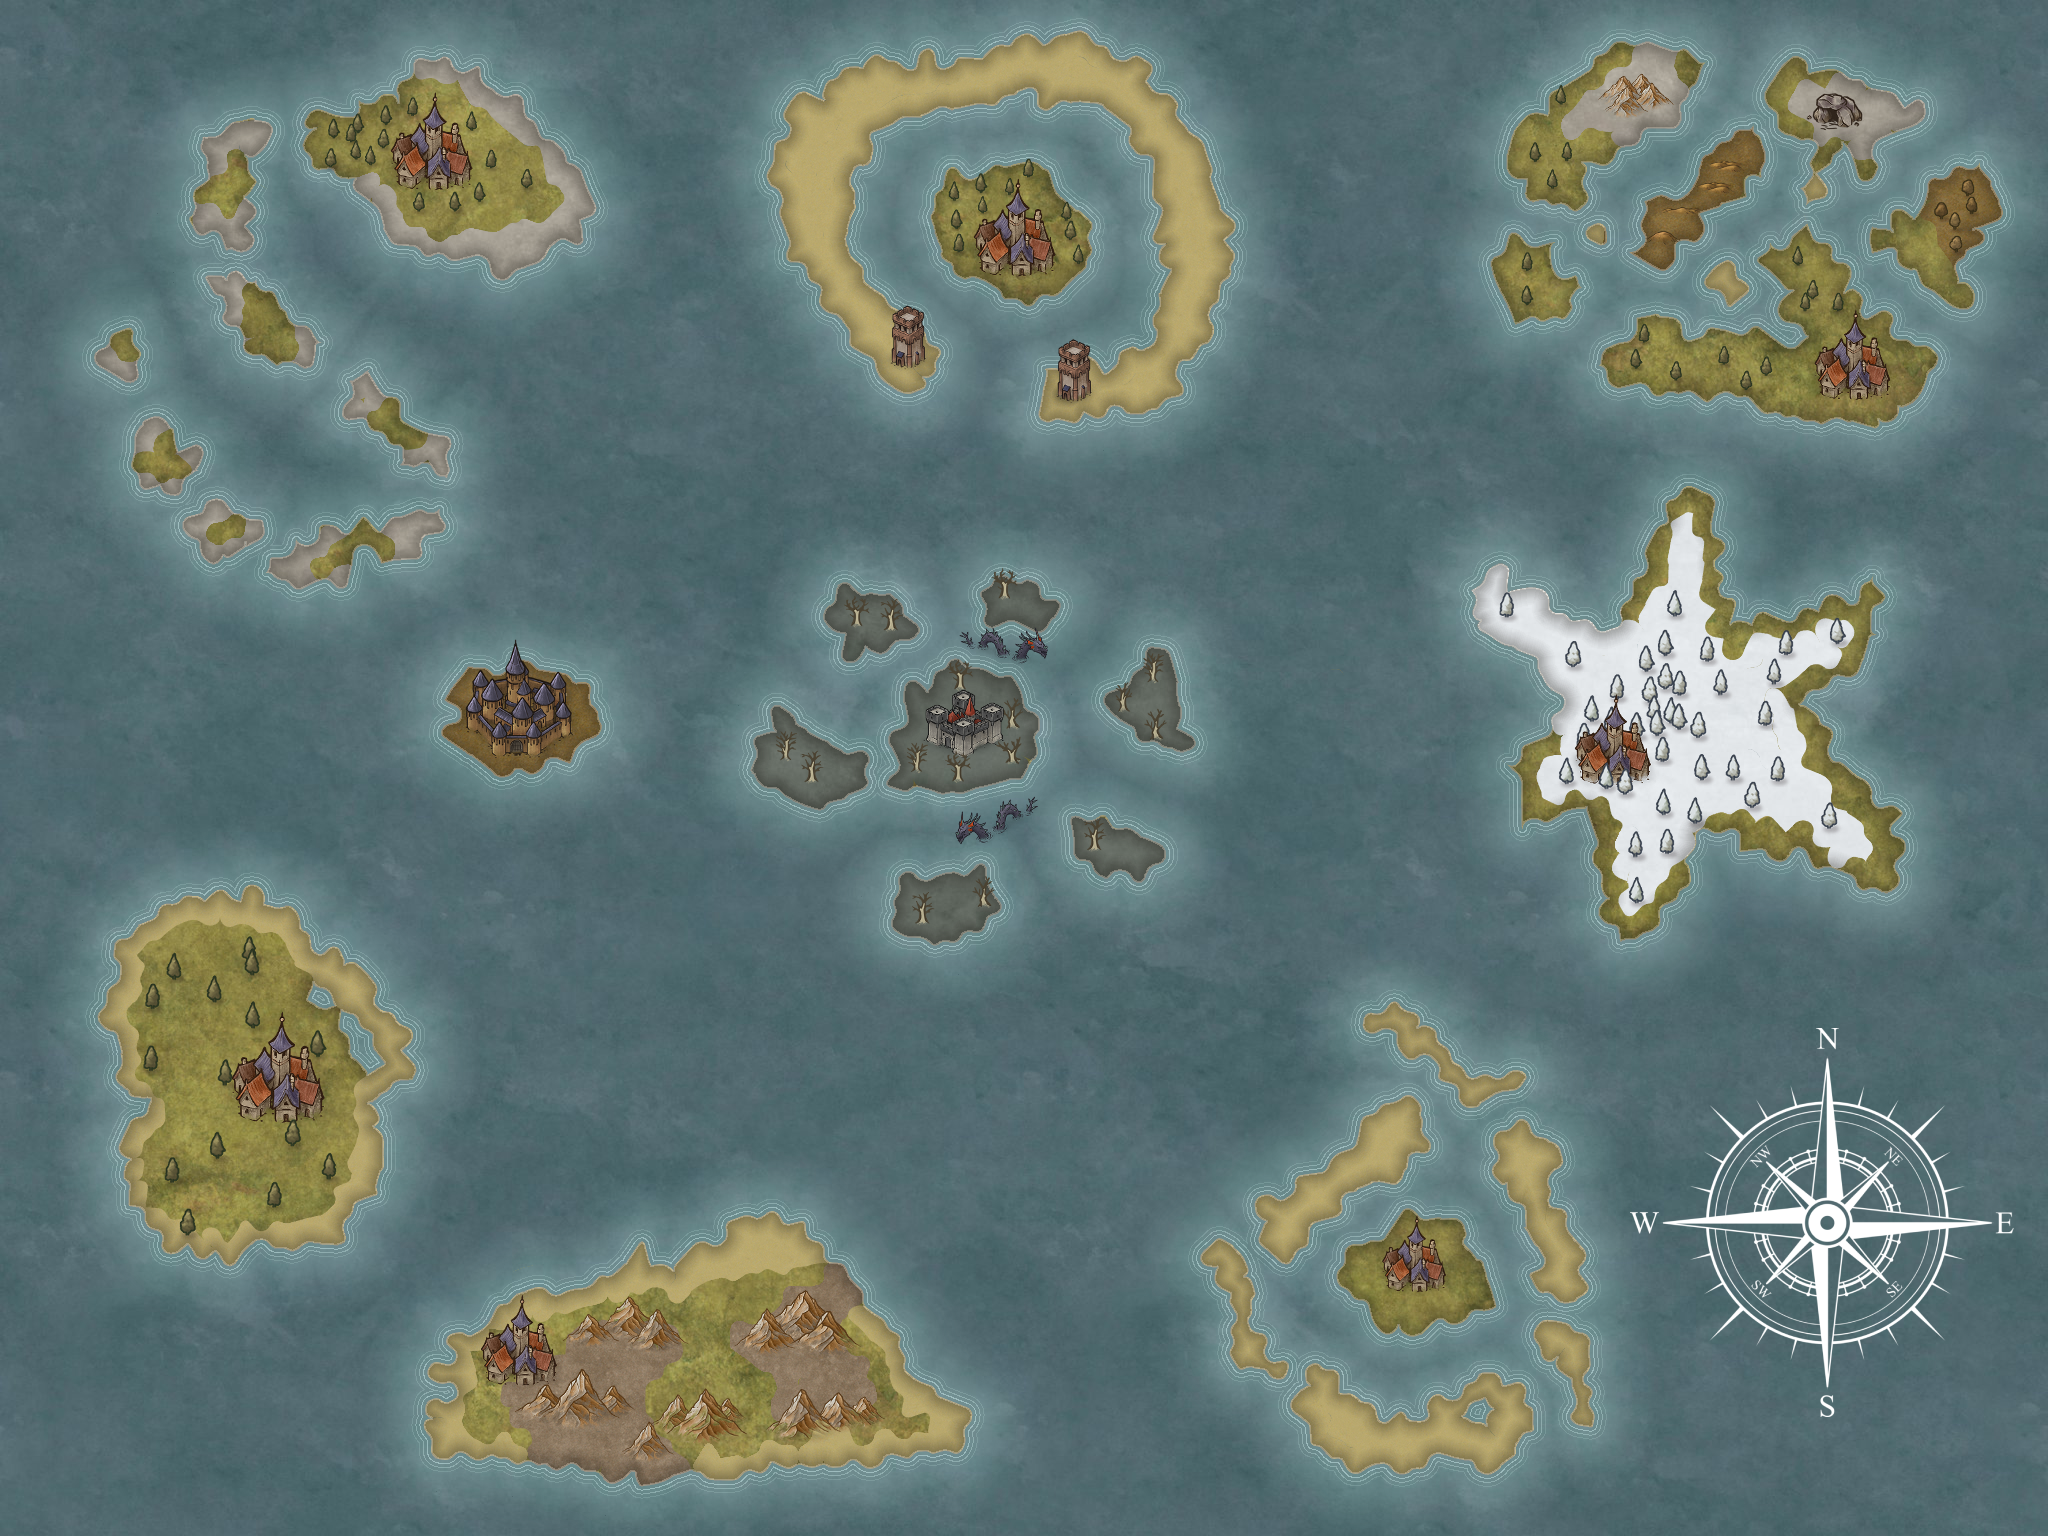
\includegraphics[width=5in]{Illustration/Map/2dMap.png}
\end{center}

Once the terrain's shape and height were refined, textures were applied using Unity's terrain painting tools. Materials such as grass, dirt, roads, and rock were painted in accordance with the original zones marked on the 2D map to preserve spatial accuracy and enhance visual coherence.\\

\begin{center}
    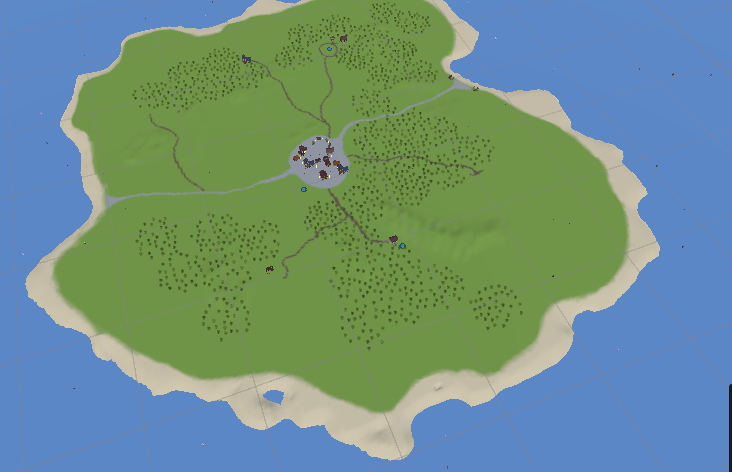
\includegraphics[width=3in]{Illustration/Map/Island.png}
\end{center}

With the terrain and textures in place, buildings and structures were strategically placed. Each island's main town was established by positioning central market areas and shops, which serve as community hubs. Surrounding these centers, houses and smaller dwellings were added based on the 2D map's layout to create believable, inhabited environments.\\

\begin{center}
    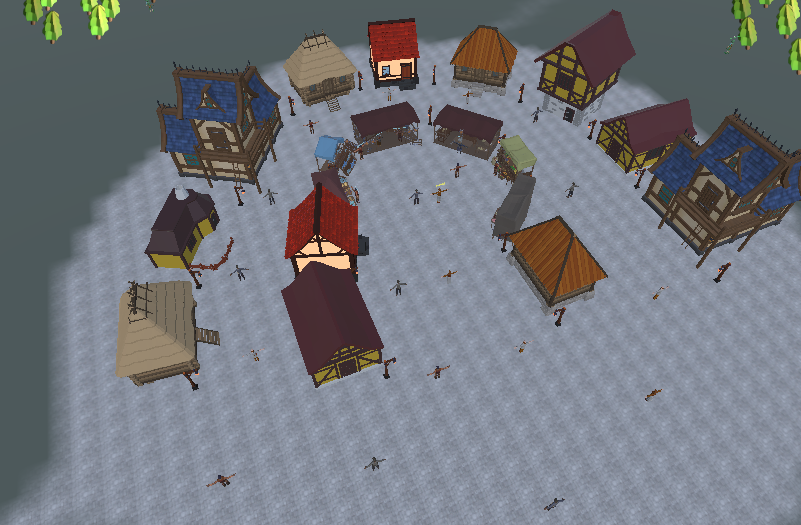
\includegraphics[width=5in]{Illustration/Map/Village.png}
\end{center}

Further environmental details such as roads, pathways, trees, and decorative elements were incorporated to support player navigation and enrich immersion. These details contributed to a vibrant and lived-in world.\\

\begin{center}
    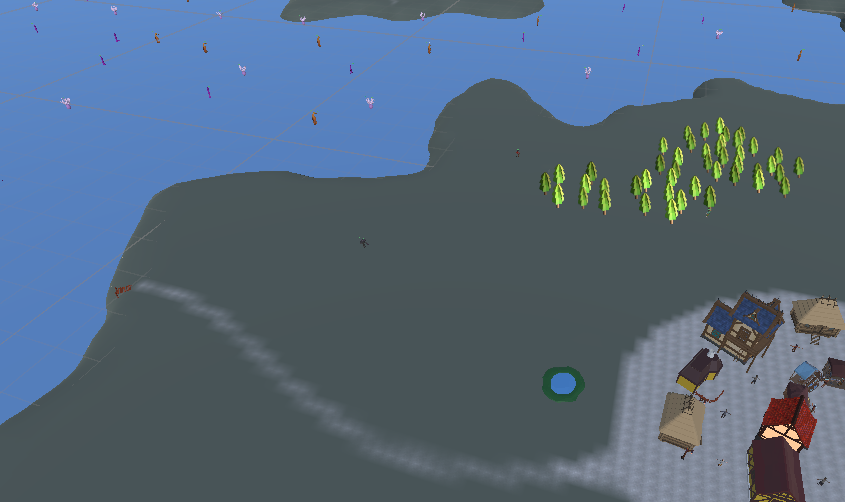
\includegraphics[width=5in]{Illustration/Map/Other.png}
\end{center}

Finally, gameplay systems were integrated into the environment. Prefabs for NPCs (passive and hostile), shops, and quest givers were placed at designated locations within towns and across islands. This ensured the map was not only visually complete but also fully functional, supporting combat, interaction, and quest progression.

\paragraph{Result}\hfill

The completed 3D map features eight well-defined islands, each anchored by a main town that acts as a central hub. Towns include shops for player interaction, passive NPCs to populate the world, and quest NPCs to guide gameplay progression. Hostile NPCs are also positioned throughout the islands to provide combat challenges.\\

Environmental decorations like trees, lanterns, and roads unify the world visually, creating a cohesive and immersive atmosphere. The careful combination of terrain design, detailed texturing, structured building placement, and gameplay integration resulted in a rich, engaging game world that faithfully recreates the original 2D map's design and enhances player exploration and interaction.

\begin{center}
    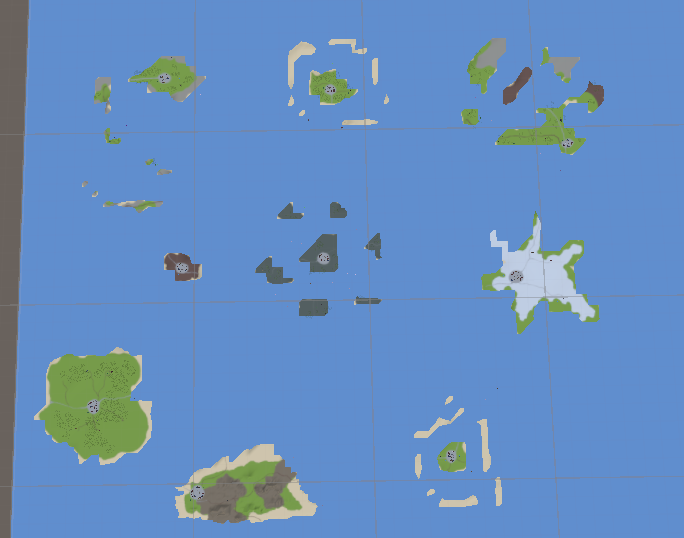
\includegraphics[width=5in]{Illustration/Map/Full.png}
\end{center}










\newpage
\subsection{Localisation system}
\paragraph{Objective}\hfill

The localization system, while essential for the player to navigate our open world, was relatively straightforward to implement. We wanted true immersion for our map, and compass. Regarding the compass, we initially planned to implement a separate object to indicate the direction the player is facing. However, we realized this would result in a heavy and slow user experience, as the map and compass could not be displayed simultaneously. We therefore decided to integrate the compass directly onto the map. \\

We also chose a less realistic approach to the compass: instead of always pointing north, the compass needle moves in the direction the player is heading. This decision was made to reduce the likelihood of the player getting lost, allowing them to focus more on the story and quests, and less on navigation. Given that the game is set in a world full of monsters and magic, we felt this choice did not significantly affect immersion. 

\paragraph{Implementation}\hfill

The UI that displays the map is a simple layer shown to the player when the map button or the M key is pressed.\\

The needle of the compass is a prefab object that tracks the player rotation along the X axis and transmits it to the compass to track which direction the player faces. 

\begin{center}
    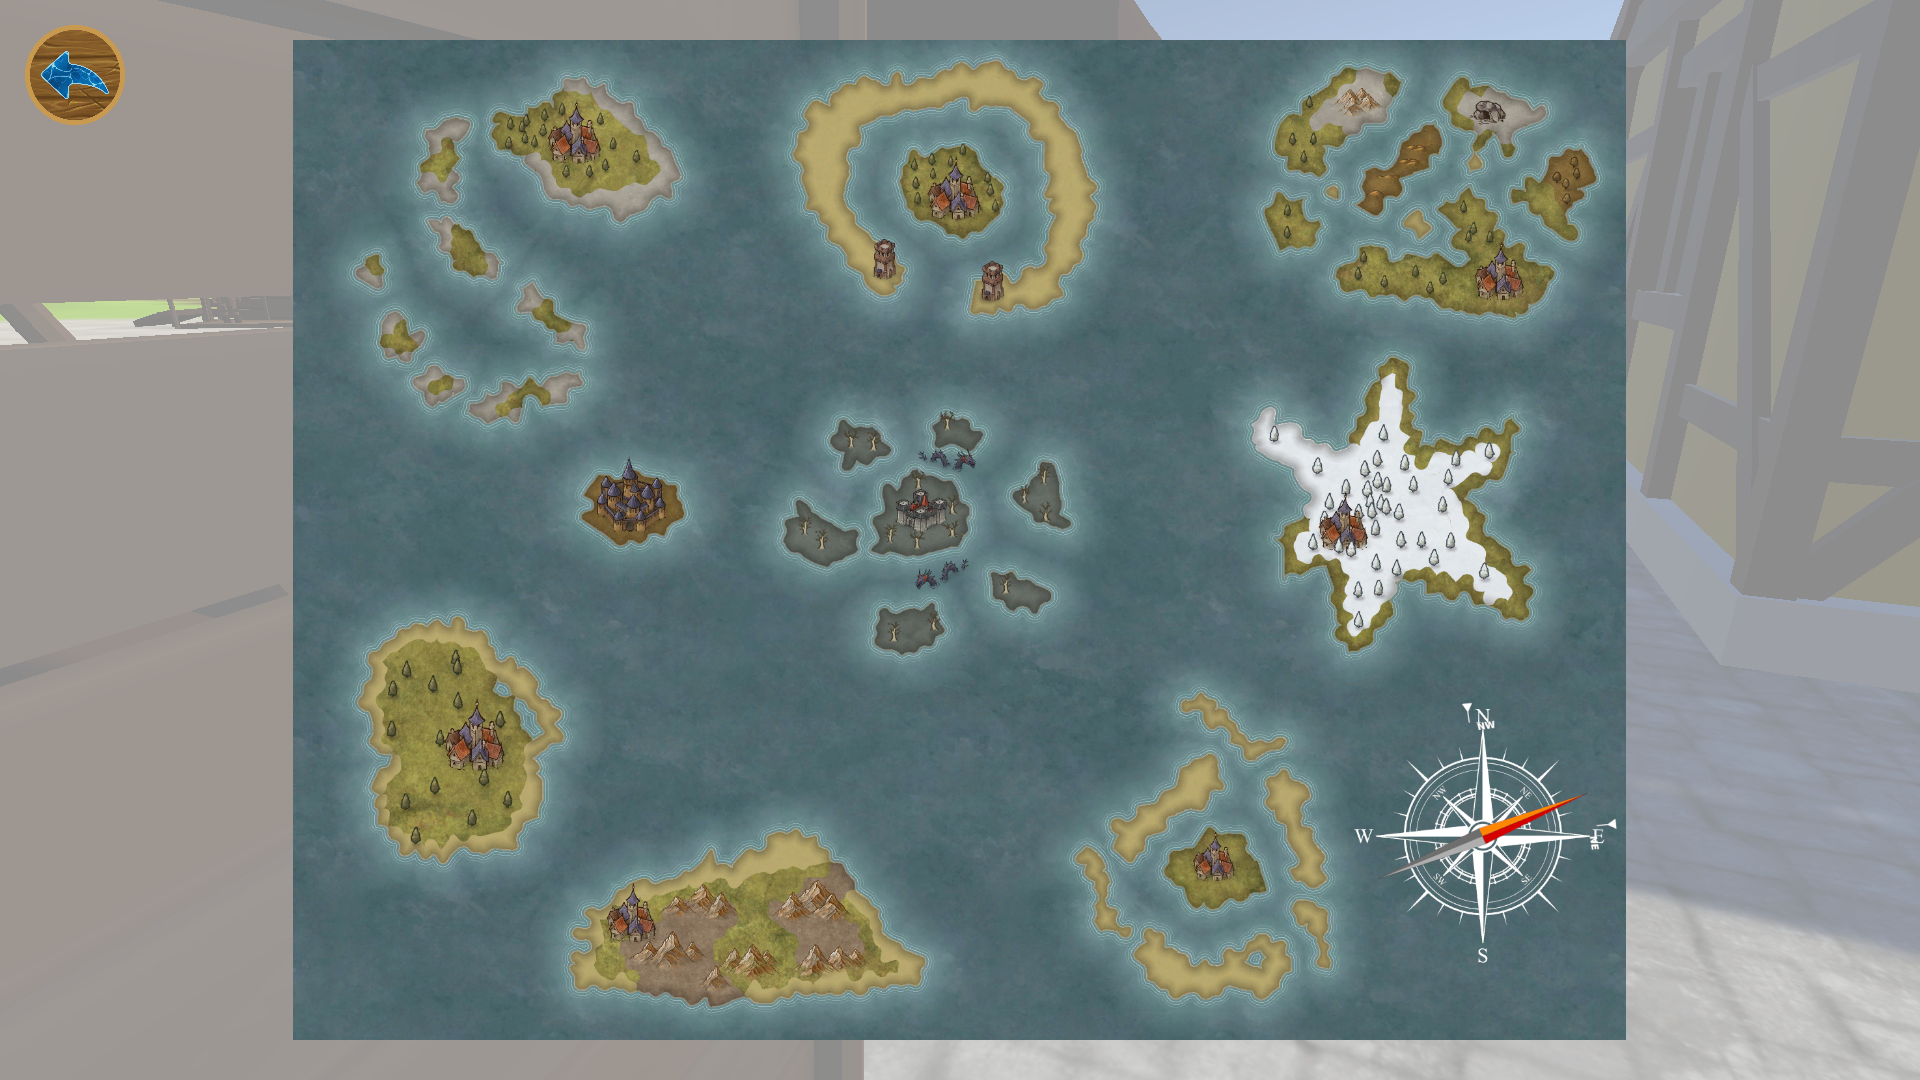
\includegraphics[width=5in]{Illustration/Localization/Loc.png}
\end{center}

\paragraph{Results}\hfill

Both the map and the compass feel immersive, quick, easy to use while conserving the authenticity of real-world map (like not giving away the player's position) so the experience is still fun and focused on exploration.










\newpage
\subsection{Implementation of Items}
\paragraph{Objective}\hfill

The primary objective was to comprehensively list and define all the objects that would appear in the game. This included a diverse range of items such as weapons, sigils, ships, crew members, and various materials. A major goal was to create original and captivating names for each item, followed by establishing player and item statistics to ensure balanced gameplay progression and immersive player experience.

\paragraph{Implementation}\hfill

The development began with extensive creative research to generate fitting names for the game's numerous objects, a process that took longer than expected but resulted in a cohesive and engaging collection of item names. This data was then organized into a JSON file, taking advantage of familiarity with JSON formatting to streamline the process.\\

Subsequently, player base statistics were defined in an Excel document, setting levels up to 100 and determining the materials required for leveling up. Developing suitable formulas to model player stat growth involved exploring both exponential and linear growth models, requiring in-depth online research. Using these formulas, item statistics were also established, with adjustments made to maintain alignment and balance with player stats.\\

Data from Excel was exported to CSV format to enable integration with Unity. To manage the game objects within Unity, scripts were written to handle both JSON and CSV data using popular libraries Newtonsoft.Json and CsvHelper. This phase required careful study of the libraries' documentation and tutorials, especially to overcome challenges with JSON parsing and script execution order within Unity's MonoBehaviour environment.\\

\begin{center}
    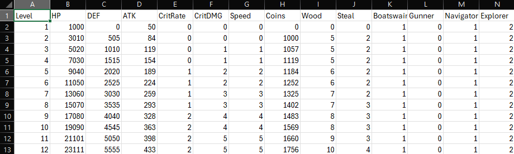
\includegraphics[width=3in]{Illustration/Items/itemData1.png}
    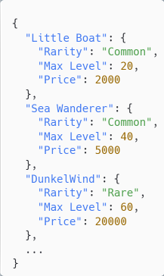
\includegraphics[width=1in]{Illustration/Items/itemData2.png}
\end{center}

For player data management, Firebase Realtime Database was initially considered but later discarded due to library incompatibility. Instead, a local JSON file approach was implemented to store essential player data such as position, level, and inventory. The inventory structure clearly distinguished between equipped and stored items, which was critical for correctly applying gameplay effects.\\

A dedicated script was developed to load player data from the JSON file and convert it into usable C\# objects. This script recalculated player statistics dynamically based on equipped weapons and sigils, integrating seamlessly with the earlier systems for game object data loading.

\paragraph{Result}\hfill

The process resulted in a well-structured and comprehensive database of game objects, complete with original names and balanced statistics that underpin player progression and item functionality. The successful integration of JSON and CSV data handling within Unity established a robust system for loading and managing game data.\\

The local JSON-based player data storage system proved reliable and efficient, enabling accurate tracking of player position, level, and inventory state. The dynamic recalculation of player stats in response to equipped items enhanced gameplay responsiveness and immersion.\\

This milestone represented a crucial step toward the game's completion, uniting diverse components into a coherent, functioning system and reinforcing the project's overall vision and momentum.










\newpage
\subsection{Shops}
\paragraph{Objective}\hfill

The primary objective of the shop system was to introduce a structured, intuitive interface that allows players to buy and sell in-game items, thereby supporting progression, strategic planning, and resource management. By establishing a functional in-game economy, the system enhances immersion and adds meaningful depth to the gameplay. The system also supports player agency by offering multiple avenues for acquiring equipment, resources, and allies critical for survival, exploration, and combat.\\

To serve this goal, six distinct shop types were designed - each tailored to fulfill a specific role within the economy and support diverse player needs.

\paragraph{Implementation}\hfill

The shop system was built around six unique merchant types, each with specialized inventories and purposes:
\begin{itemize}
    \item \textbf{Armorer}: Offers melee and ranged weapons.
    \item \textbf{Boat Salesman}: Provides various boats for travel and combat.
    \item \textbf{Mage}: Sells magical sigils and enchantments.
    \item \textbf{Crew Agent}: Enables the recruitment of crew members.
    \item \textbf{Material Merchant}: Supplies raw crafting materials such as steel, wood, and Pure Water Drops.
    \item \textbf{Purchaser}: Allows players to offload unused items for currency or materials.
\end{itemize}

Each merchant was implemented as an interactable NPC prefab, featuring unique visual designs. These prefabs were positioned throughout the game world in key locations to ensure logical access during gameplay.\\

\begin{center}
    
\includegraphics[width=5in]{Illustration/Shops/Shop1.png}
    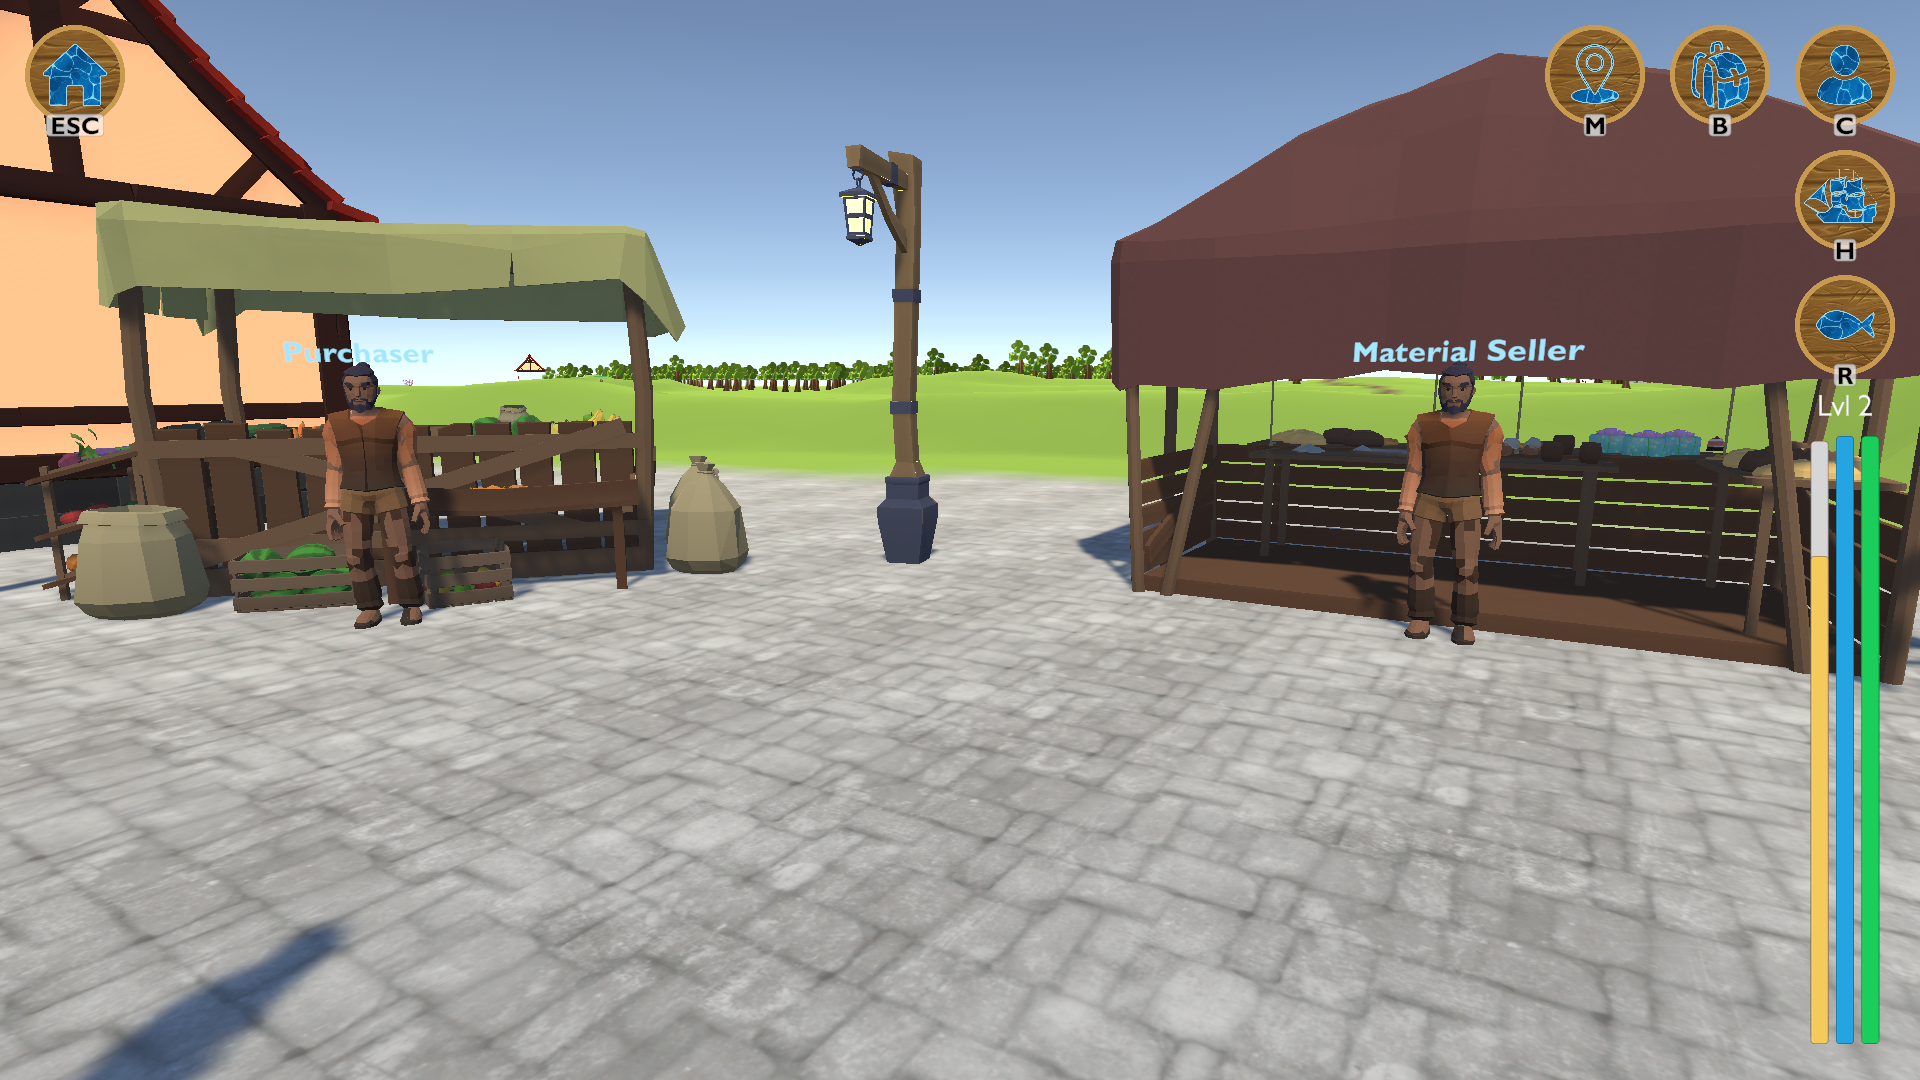
\includegraphics[width=5in]{Illustration/Shops/Shop2.png}
\end{center}

Interaction with merchants was enabled using Unity's raycasting system, allowing players to trigger specific shop menus by clicking on NPCs. Each merchant prefab includes a category identifier, which dynamically loads the corresponding inventory when accessed.\\

A unified shop UI was created for all merchant types, promoting visual consistency and intuitive navigation. The shared interface includes:
\begin{itemize}
    \item Item Scroll View: Displays merchant-specific items.
    \item Item Description Panel: Shows item details (e.g., stats, rarity, material costs).
    \item Player Resources Display: Reflects current coin, material, and Pure Water Drop counts.
    \item Buy/Sell Buttons: Executes the appropriate transaction logic based on the shop type.
\end{itemize}

The modular UI structure allowed for easy adaptation between shop types, with backend scripts dynamically populating the item list based on the interacting merchant.\\

The shop system was built on top of the existing inventory infrastructure, allowing for efficient reuse of scripts and interfaces. Key enhancements included:
\begin{itemize}
    \item Buy Logic: Checks player resource availability before confirming purchases. Successful transactions add the item to the player's inventory and deduct the appropriate cost.
    \item Sell Logic: Displays all inventory items in the Sell Menu. Items can be sold for coins or materials, freeing inventory space and rewarding players with resources.
    \item Real-Time UI Updates: Ensures immediate feedback on transactions, reflecting changes to inventory and resource values.
\end{itemize}

Inventory data was managed through scriptable objects and categorized item databases. These databases were referenced at runtime based on the merchant type, enabling dynamic population of each merchant's offerings without hardcoded lists.\\

\begin{center}
    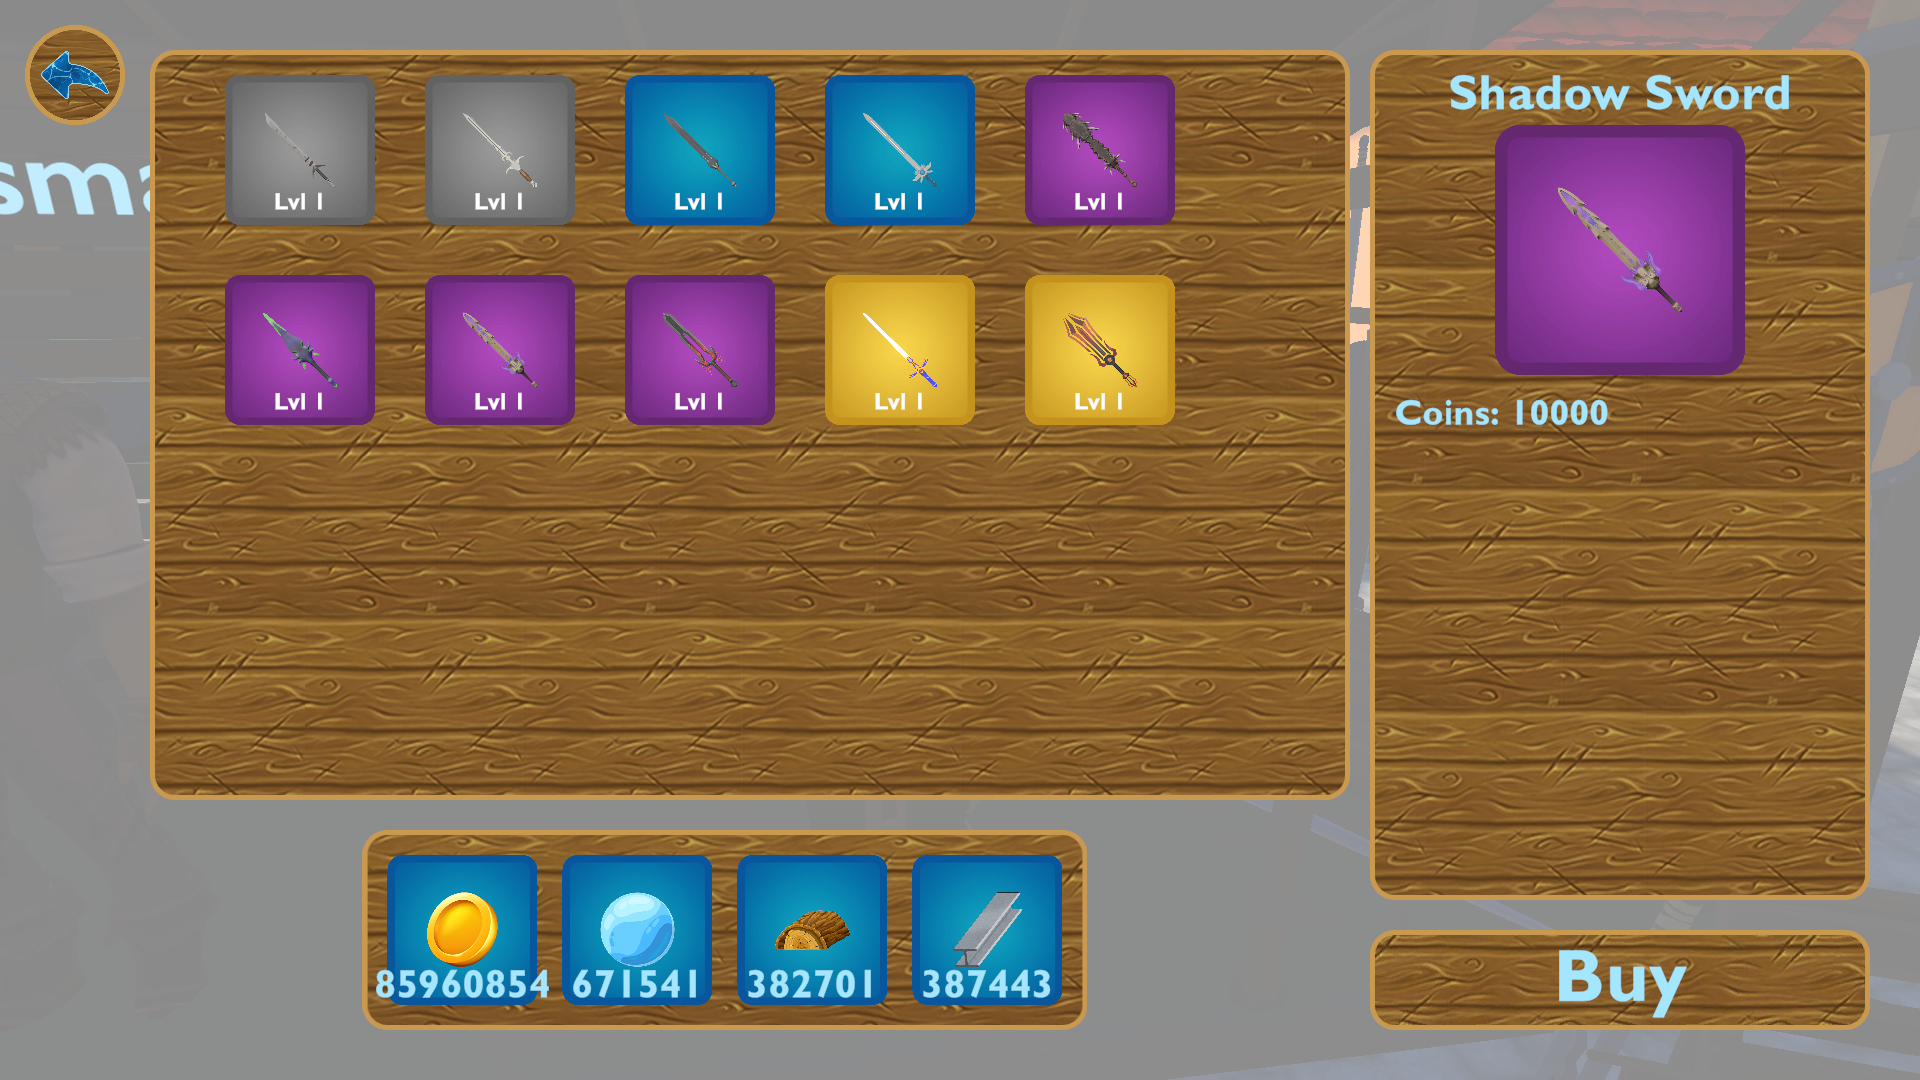
\includegraphics[width=4in]{Illustration/Shops/Armorer.png}
\end{center}

During development, it became evident that players lacked a reliable way to acquire core crafting materials. To resolve this, the Material Merchant was introduced. This shop type followed the same UI and prefab structure but was connected to a materials-specific item database. It provided access to critical upgrade components and allowed for more balanced pacing in player progression.\\

\begin{center}
    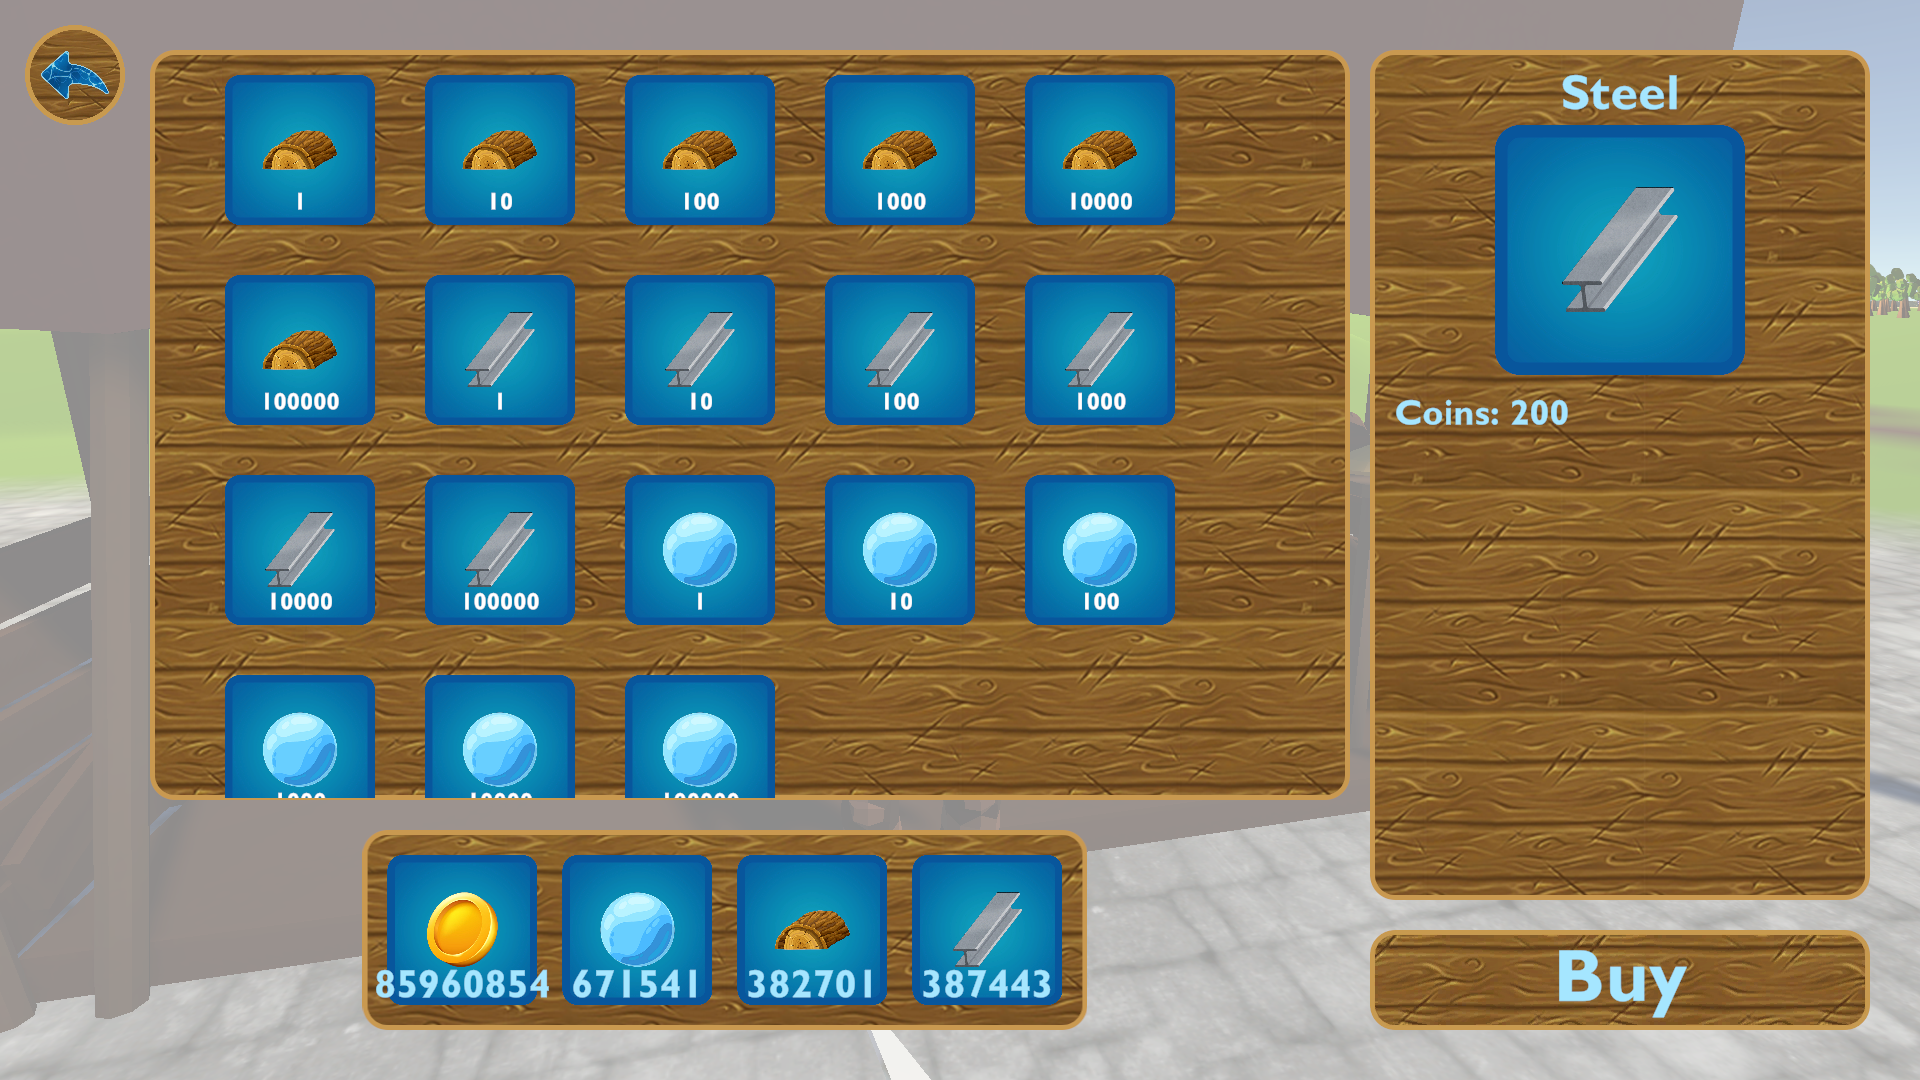
\includegraphics[width=4in]{Illustration/Shops/MaterialsSeller.png}
\end{center}

Similarly, the Sell Merchant was created to complete the economic loop. The sell system reused the inventory UI, replacing the Upgrade button with a Sell button that removed the item from the inventory and rewarded the player accordingly. Sell values were predefined based on item rarity and category.\\

\begin{center}
    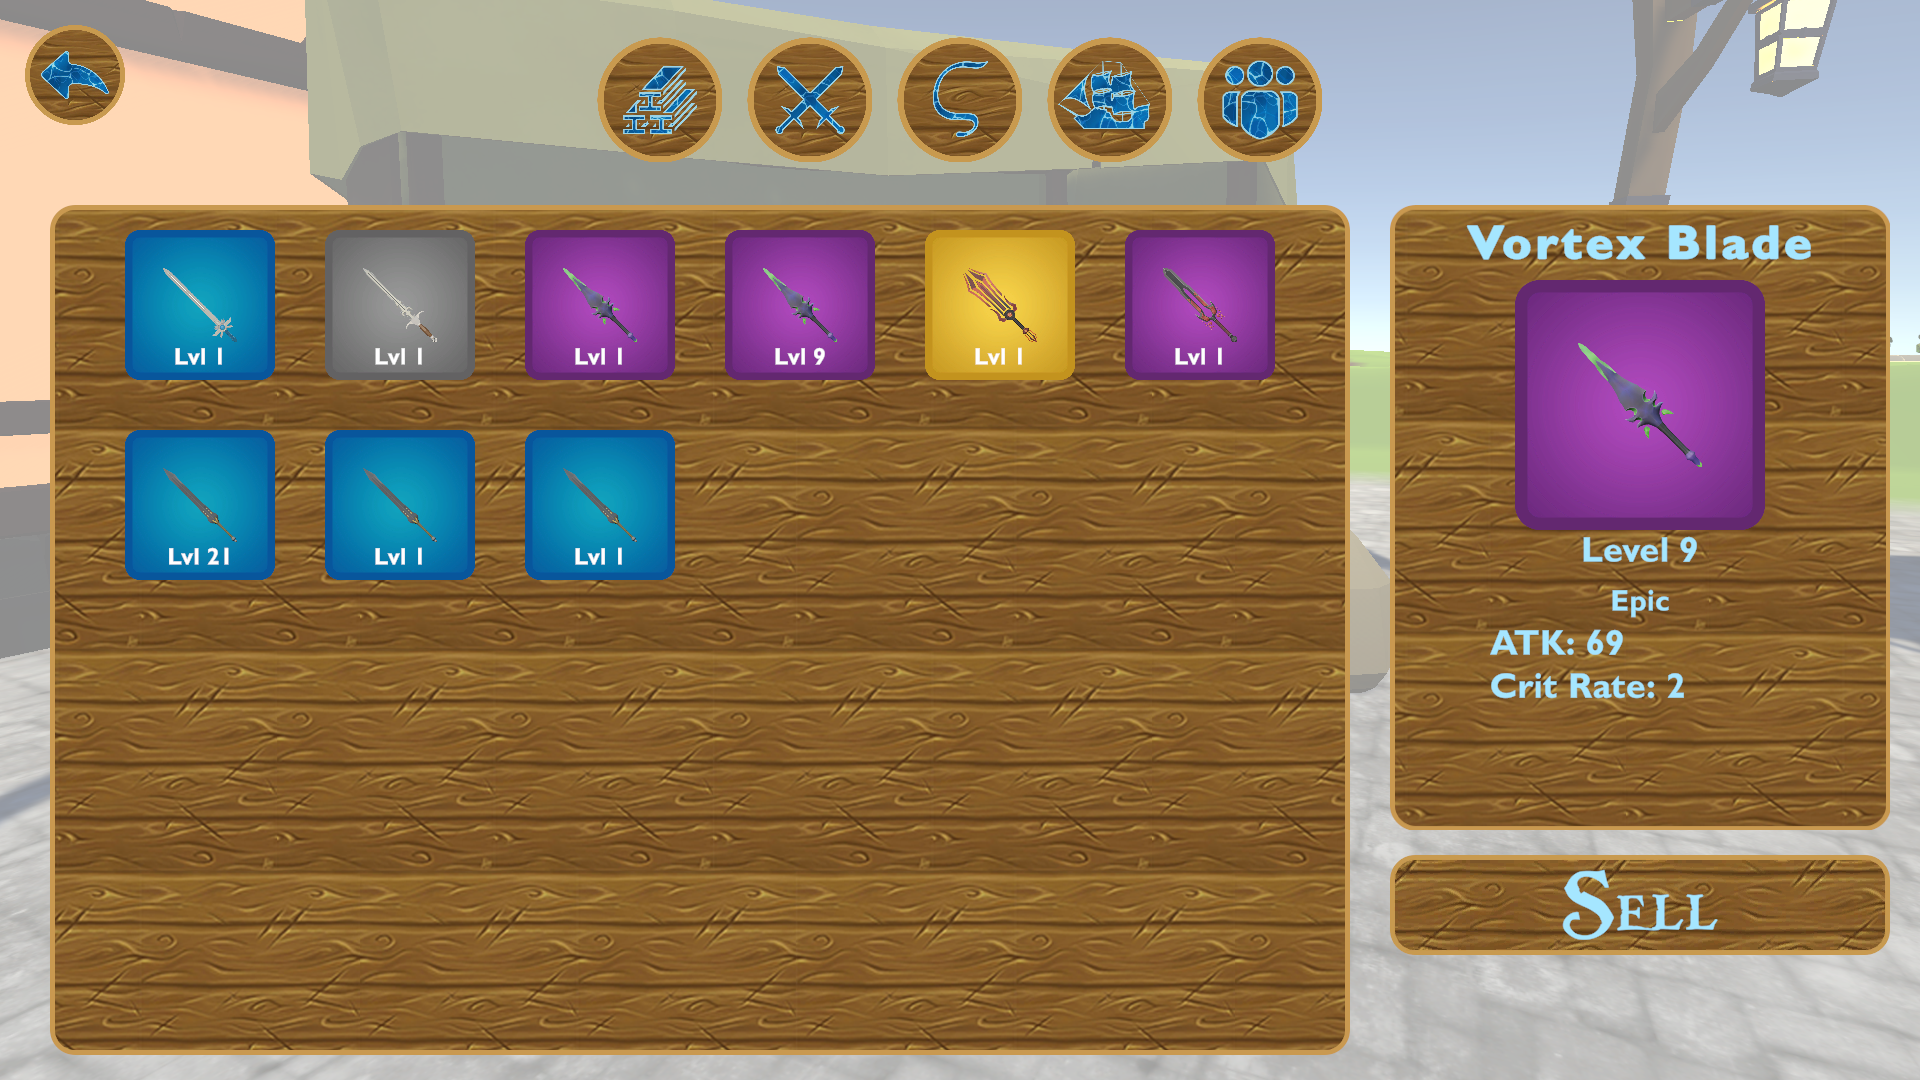
\includegraphics[width=4in]{Illustration/Shops/Purchaser.png}
\end{center}

Both new shop types were implemented efficiently due to the modularity of the shop UI and the flexible inventory system, requiring only minor adjustments to existing scripts.

\paragraph{Result}\hfill

The fully implemented shop system introduced a diverse and meaningful layer of interactivity to the game's economic structure. With six distinct shop types covering equipment, magic, transport, personnel, resources, and item resale, players are empowered to make strategic decisions tailored to their playstyle and objectives.\\

Key results include:
\begin{itemize}
    \item A consistent and intuitive UI across all shop interactions.
    \item Efficient transaction handling, tied directly into the player's resource and inventory systems.
    \item Improved pacing and balance, enabled by resource merchants and resale mechanics.
    \item Enhanced immersion, driven by unique merchant NPCs and logical shop placements within the world.
\end{itemize}

This system not only enriches moment-to-moment gameplay but also lays the groundwork for potential future systems, including advanced crafting, faction-based economies, or dynamic pricing models. The modular and scalable design ensures that the shop system can evolve in complexity as the game continues to grow.








\newpage
\subsection{Fishing system}
\paragraph{Objective}\hfill

The goal of the fishing system was to introduce a unique, interactive minigame that adds variety to player activities while supporting core survival and economic mechanics. Fishing allows players to gather food to manage hunger, and also to sell caught fish for in-game currency. The system was designed to be immersive and skill-based, creating a more dynamic and rewarding gameplay experience within the game world.

\paragraph{Implementation}\hfill

The fishing mechanic was initially conceptualized as a reaction-based minigame triggered by player interaction with fishing ponds located throughout the game world. The core gameplay involved clicking on moving fish to catch them, with each fish moving unpredictably to challenge the player's reflexes and accuracy.\\

The first prototype was implemented in a 3D environment. A fixed camera faced the pond as five fish moved laterally using sinusoidal motion, achieved with Mathf.Sin() in Unity. Fish were recycled to the left side of the screen upon reaching the right boundary to maintain gameplay flow. Extensive testing determined that five fish provided an ideal balance between difficulty and accessibility.\\

After evaluating performance and user interaction, the system was reworked using Unity's 2D Canvas UI for better precision and optimization. Fish were converted into clickable UI Buttons, improving input responsiveness and simplifying detection logic using Unity's built-in UI system.\\

This required converting GameObjects from Transform to RectTransform, and adjusting movement logic to function within the UI layout. Movement speed and screen boundaries were recalibrated to suit the 2D space, maintaining smooth and natural animation within the interface.\\

To reward the player and support game progression, the inventory system was updated to include fish as a new item type. Upon each successful click, the player's fish count was incremented via a dedicated inventory function.\\

A real-time fish counter UI element was also added to the interface. It updated instantly upon catching a fish, providing satisfying feedback and reinforcing a sense of achievement.\\

Initially, caught fish were removed from the scene, gradually reducing the number of targets. This disrupted the gameplay flow and required players to restart the minigame. The mechanic was revised so that new fish spawned immediately upon a successful catch, creating a seamless and continuous fishing experience.\\

Three 3D fish models were sourced from the Unity Asset Store. Since the Canvas system required 2D visuals, these models were converted into sprites using Blender. Renders were exported as high-resolution PNGs and imported into Unity, resulting in visually distinct and appealing UI elements for the minigame.\\

\begin{center}
    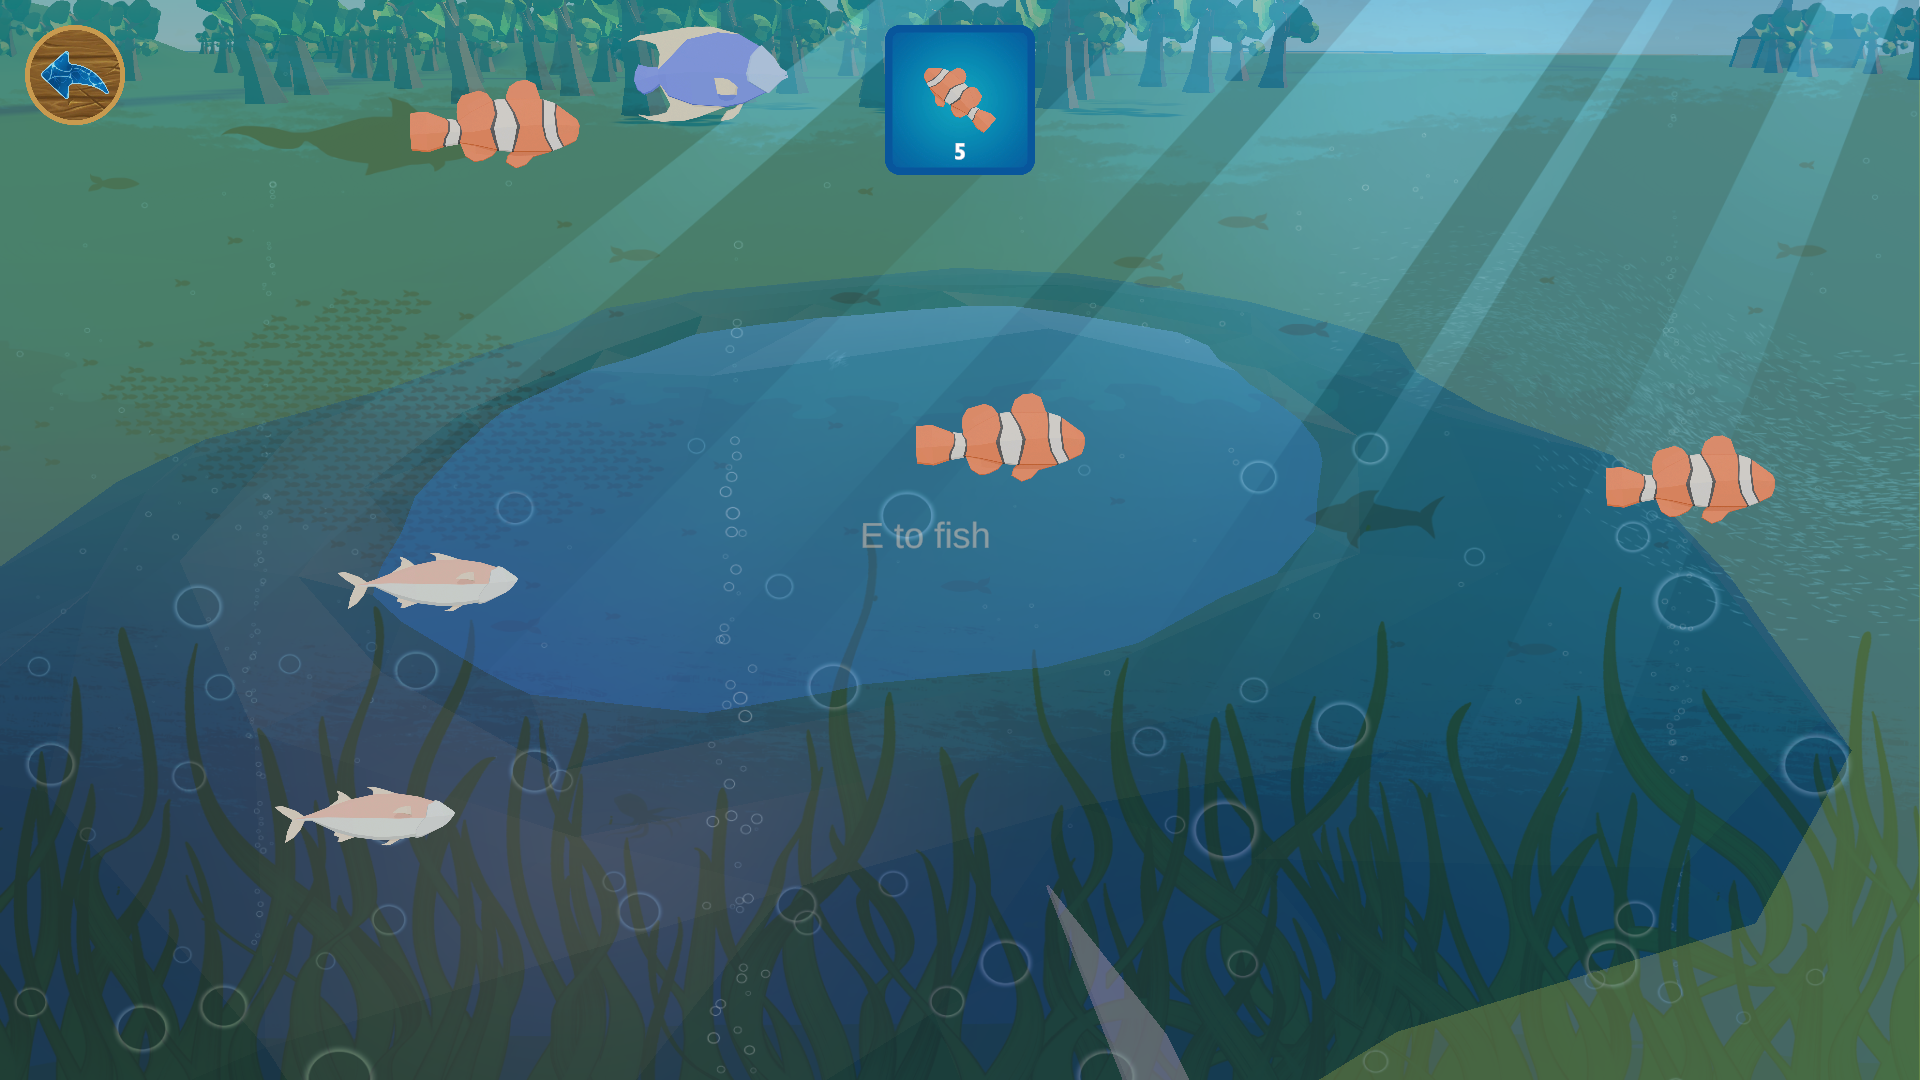
\includegraphics[width=4in]{Illustration/Fishing/Fishing.png}
\end{center}

Fishing ponds were strategically placed across multiple islands, allowing players to access the minigame during exploration. Interaction with these ponds activated the fishing interface, smoothly transitioning players into the minigame environment.

\begin{center}
    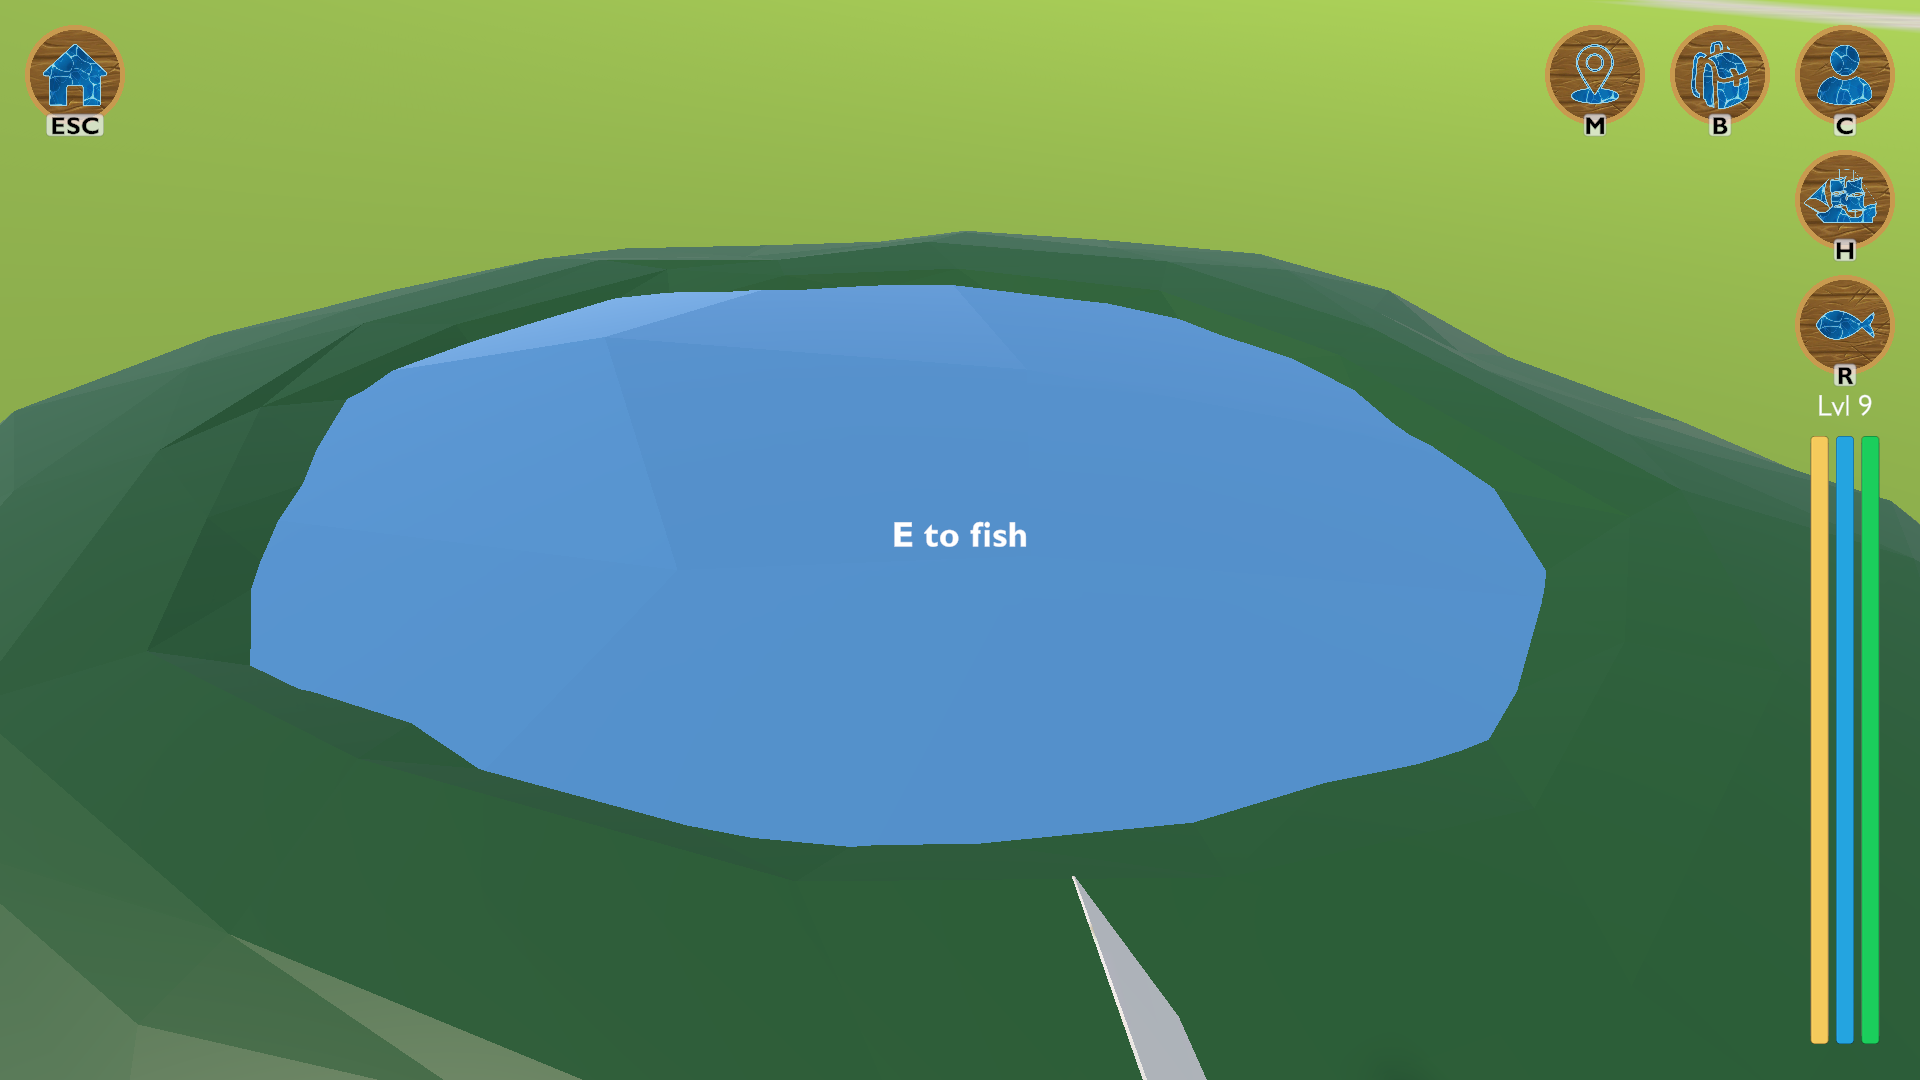
\includegraphics[width=4in]{Illustration/Fishing/Pond.png}
\end{center}

\paragraph{Result}\hfill

The fishing system successfully introduced an engaging and skill-based gameplay feature that complements both survival and exploration mechanics. Its transition from a 3D to a 2D interface resulted in improved performance, intuitive input, and polished visuals.\\

The system's tight integration with the inventory and UI provided immediate feedback, enhancing player agency and reinforcing a sense of progression. Real-time counters and seamless spawning mechanics ensured a smooth and satisfying gameplay loop.\\

Overall, the fishing minigame enriched the world with an enjoyable side activity that deepened immersion and offered strategic value, solidifying its role as a meaningful and well-integrated feature in the game's broader design.










\newpage
\subsection{Network}
\paragraph{Objective}\hfill

The objective of this task was to synchronize player movement and interactions with boats in a multiplayer environment. The network system of the game utilizes Unity's Netcode for GameObjects (NGO), a networking library designed for building multiplayer games. NGO allows for the synchronization of GameObjects—such as player characters, boats, treasure chests, and flags—across both clients and the server. In this project, synchronization was specifically implemented for players, boats, and other essential GameObjects, including the Treasure Chest in Treasure Hunt mode and the Flag in Boat Race mode.

\paragraph{Implementation}\hfill

The first step involved creating a simple Network HUD interface with two buttons:\
\begin{itemize}
    \item Client - Connects the user as a client.
    \item Host - Connects the user as a host to the local server.
\end{itemize}

This setup provided a basic yet functional interface for initiating multiplayer sessions during development and testing.\\

\begin{center}
    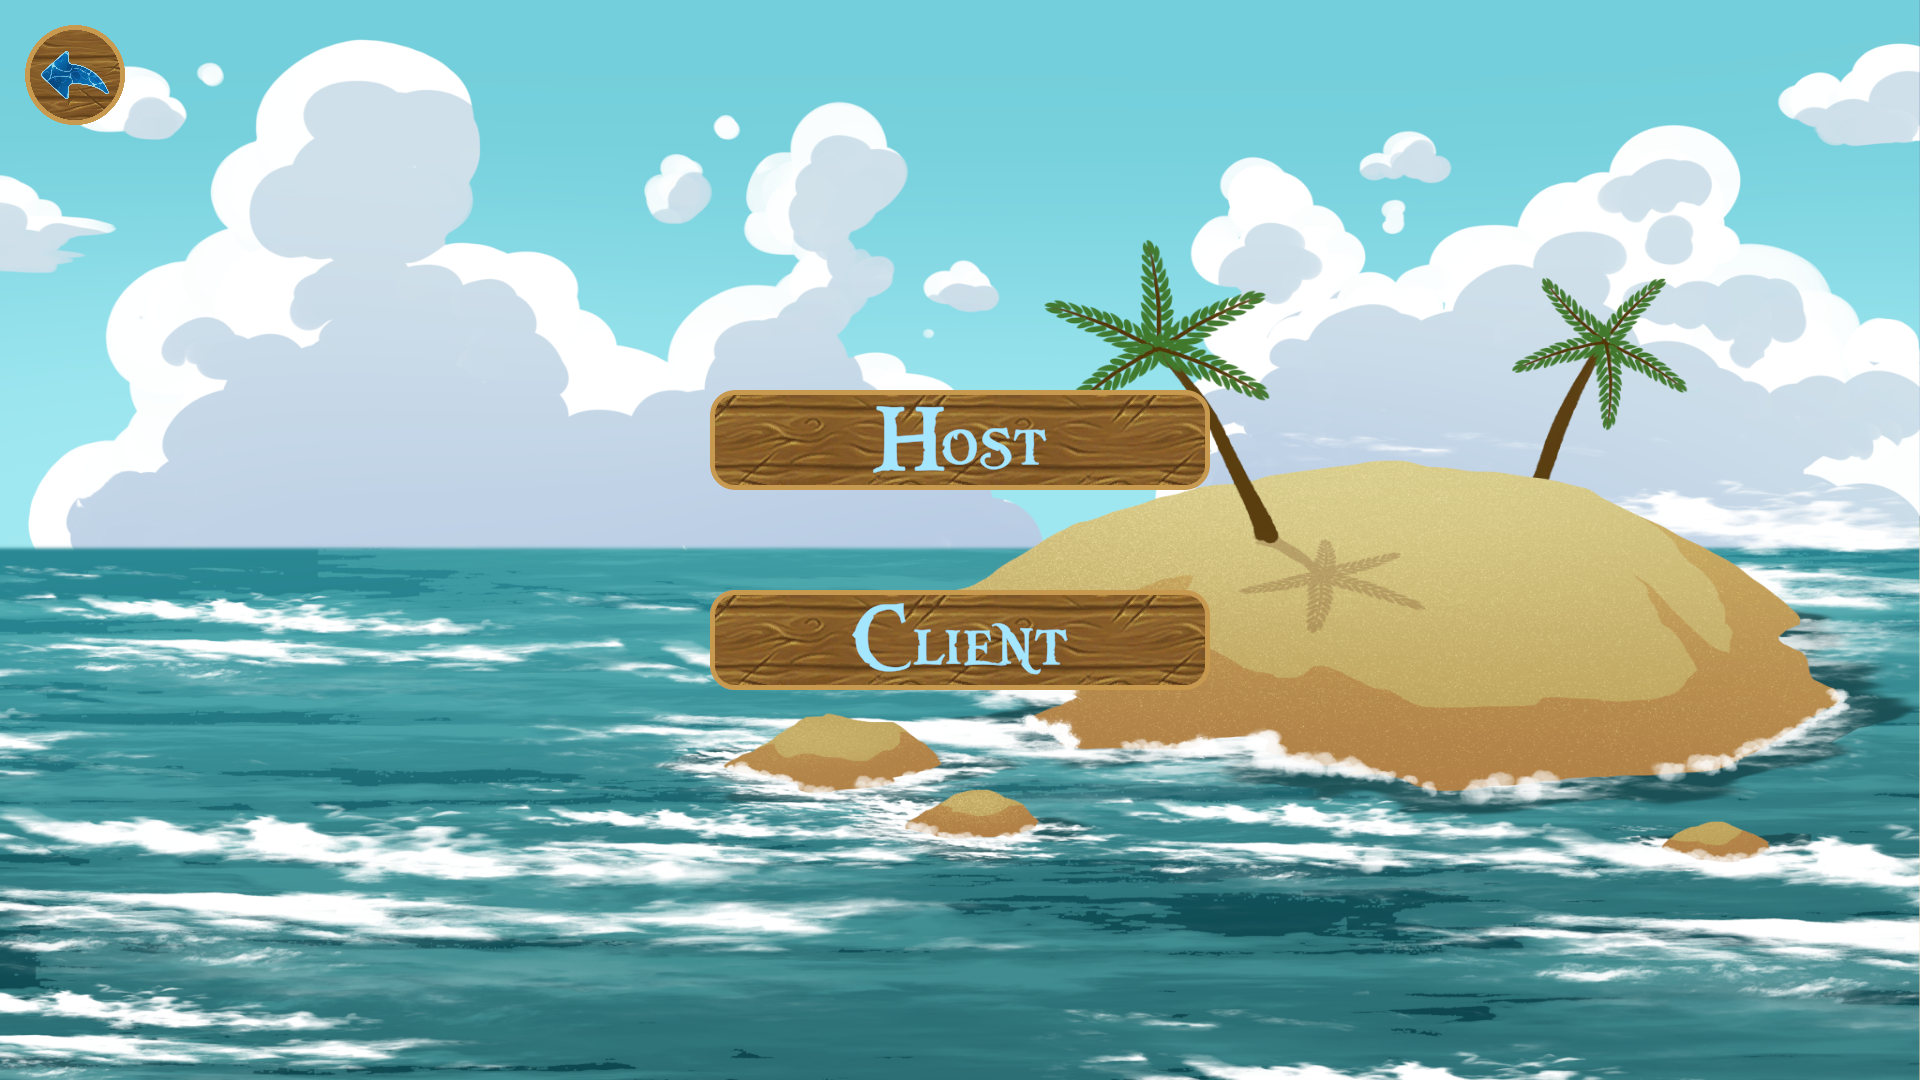
\includegraphics[width=4in]{Illustration/Network/MultiplayerHUD.png}
\end{center}

The next phase focused on synchronizing the player's position across clients. This step was time-consuming and required external resources and guidance, including tutorials such as this video \url{https://youtu.be/2OLUdPkkQPI}. Once positional synchronization was achieved, work proceeded to the synchronization of player animations.

The most challenging aspect of the implementation was synchronizing the interaction between players and boats, including boat movement. To facilitate networked behavior, the player movement and animation scripts were modified to inherit from NetworkBehaviour instead of the standard MonoBehaviour.\\

In multiplayer mode, unlike in single-player where each player owns and places their own boat via inventory, there is no player inventory system. This design choice was made to ensure fairness in minigames by removing differences in level or equipment. As a result, players interact with boats already present in the scene. This required adjustments to the interaction scripts to account for network-specific variations, ensuring accurate state replication across clients.\\

An issue was encountered where the animation of one player was not visible to other players during movement. This was initially assumed to be a network synchronization error. However, further investigation revealed it was due to how Unity's Multiplayer Play Mode handles multiple game instances. Specifically, when one instance (e.g., the host or a client) is minimized, Unity suspends the rendering and processing of that instance to optimize performance, causing animations not to appear in other players' views. This behavior is a known optimization feature, not a fault in the network implementation.

\begin{center}
    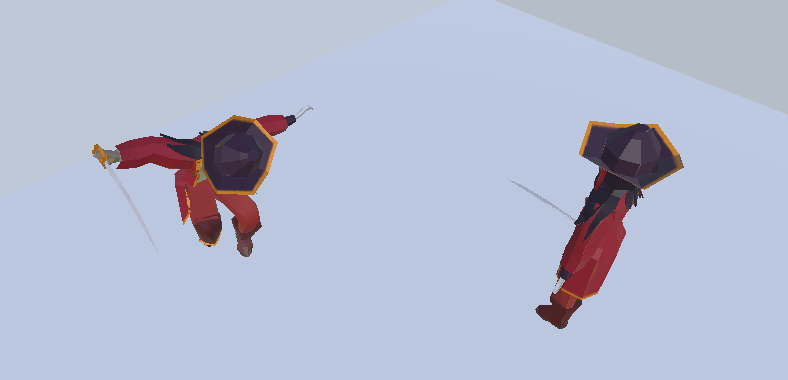
\includegraphics[width=4in]{Illustration/Network/NetworkPlayer.png}
\end{center}

\paragraph{Result}\hfill

The final implementation successfully synchronized player movement, animations, and boat interactions in a cooperative multiplayer setting. Players can now join a local server via the custom network HUD and interact with boats and other GameObjects in real time. This ensures a functional and cohesive multiplayer experience that aligns with the intended design of the game's cooperative and competitive modes.











\newpage
\subsection{Multiplayer}
\paragraph{Objectives}\hfill

The addition of multiplayer functionality aimed to expand the game experience by introducing new ways for players to engage with one another. Two mini-games were designed as optional multiplayer activities: a treasure hunt and a boat race. Both were inspired by pirate folklore and seafaring traditions, reinforcing the game's theme while offering exciting, social gameplay moments.\\

The treasure hunt mode encourages exploration and competitive discovery, where players race to find a hidden chest. Meanwhile, the boat race reflects the naval prowess of pirates, challenging players to navigate a marked course in a test of speed and control. Together, these modes were conceived to add variety, replayability, and a sense of camaraderie or rivalry to the game.

\paragraph{Implementation}\hfill

Multiplayer integration was achieved using Unity's Netcode for GameObjects (NGO), which provided the tools necessary to manage networking, synchronization, and authority across players. All players begin their multiplayer experience inside a shared lobby space—visually represented by a plain white-box environment—where they await the host's decision on which mini-game to launch. Only the host is given the ability to select the mini-game mode, reinforcing their role as the session leader. The system was designed to wait until all players were connected before transitioning to gameplay, ensuring a fair and unified start for every participant.\\

\begin{center}
    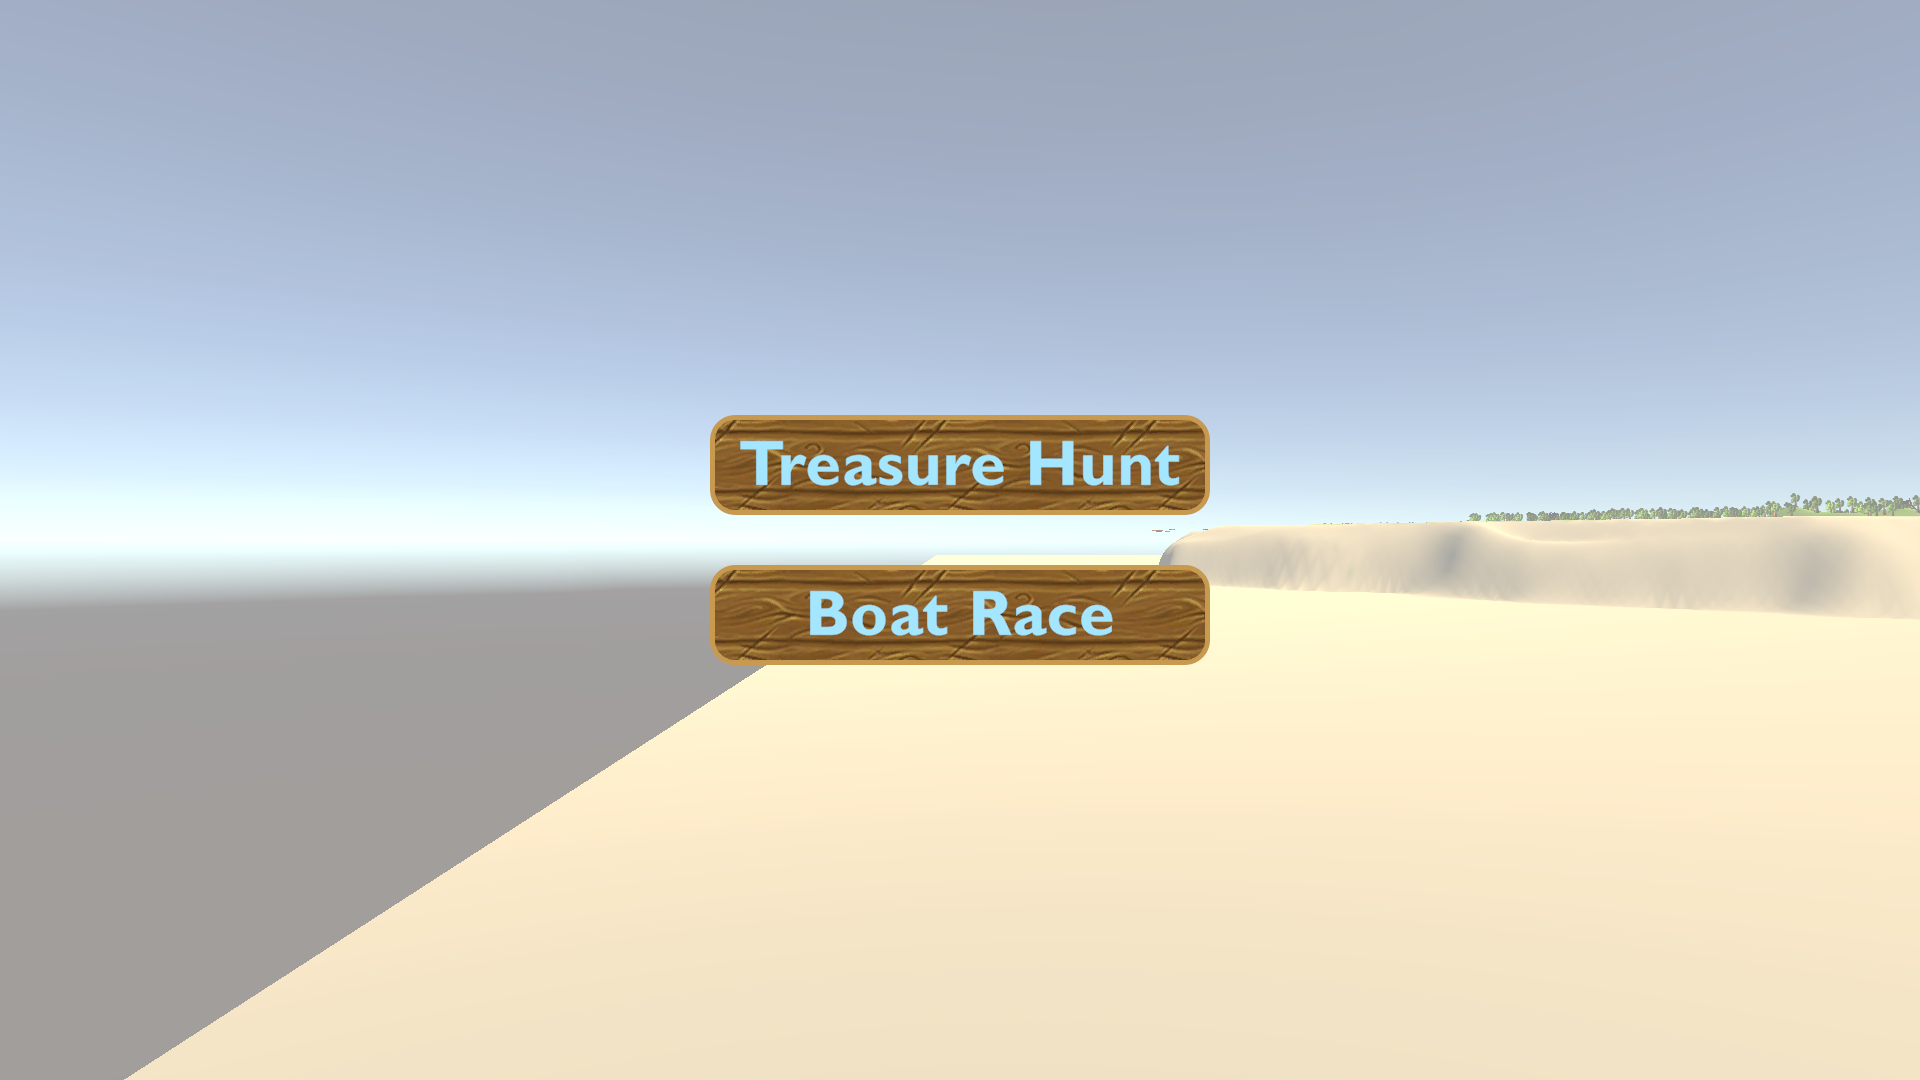
\includegraphics[width=4in]{Illustration/Multiplayer/MultiplayerChoiceModeMenu.png}
\end{center}

Transitioning players from the lobby to the mini-game locations presented an initial technical hurdle. Unity's network architecture restricts player object movement to the server, meaning that the host alone does not have permission to reposition all players. To resolve this, ServerRPCs were used to instruct the server to teleport each player to the appropriate location—whether to the center of the island for the treasure hunt or to the pier for the boat race.\\

In the treasure hunt mini-game, one chest is spawned randomly among a set of carefully chosen locations to avoid placement issues. Players are free to explore the map, guided only by a user interface element displaying the real-time distance to the chest. Once a player reaches the chest, the system declares them the winner, displaying a victory screen. Other participants are simultaneously shown a message reflecting their loss, with both screens offering the option to disconnect from the session.\\

\begin{center}
    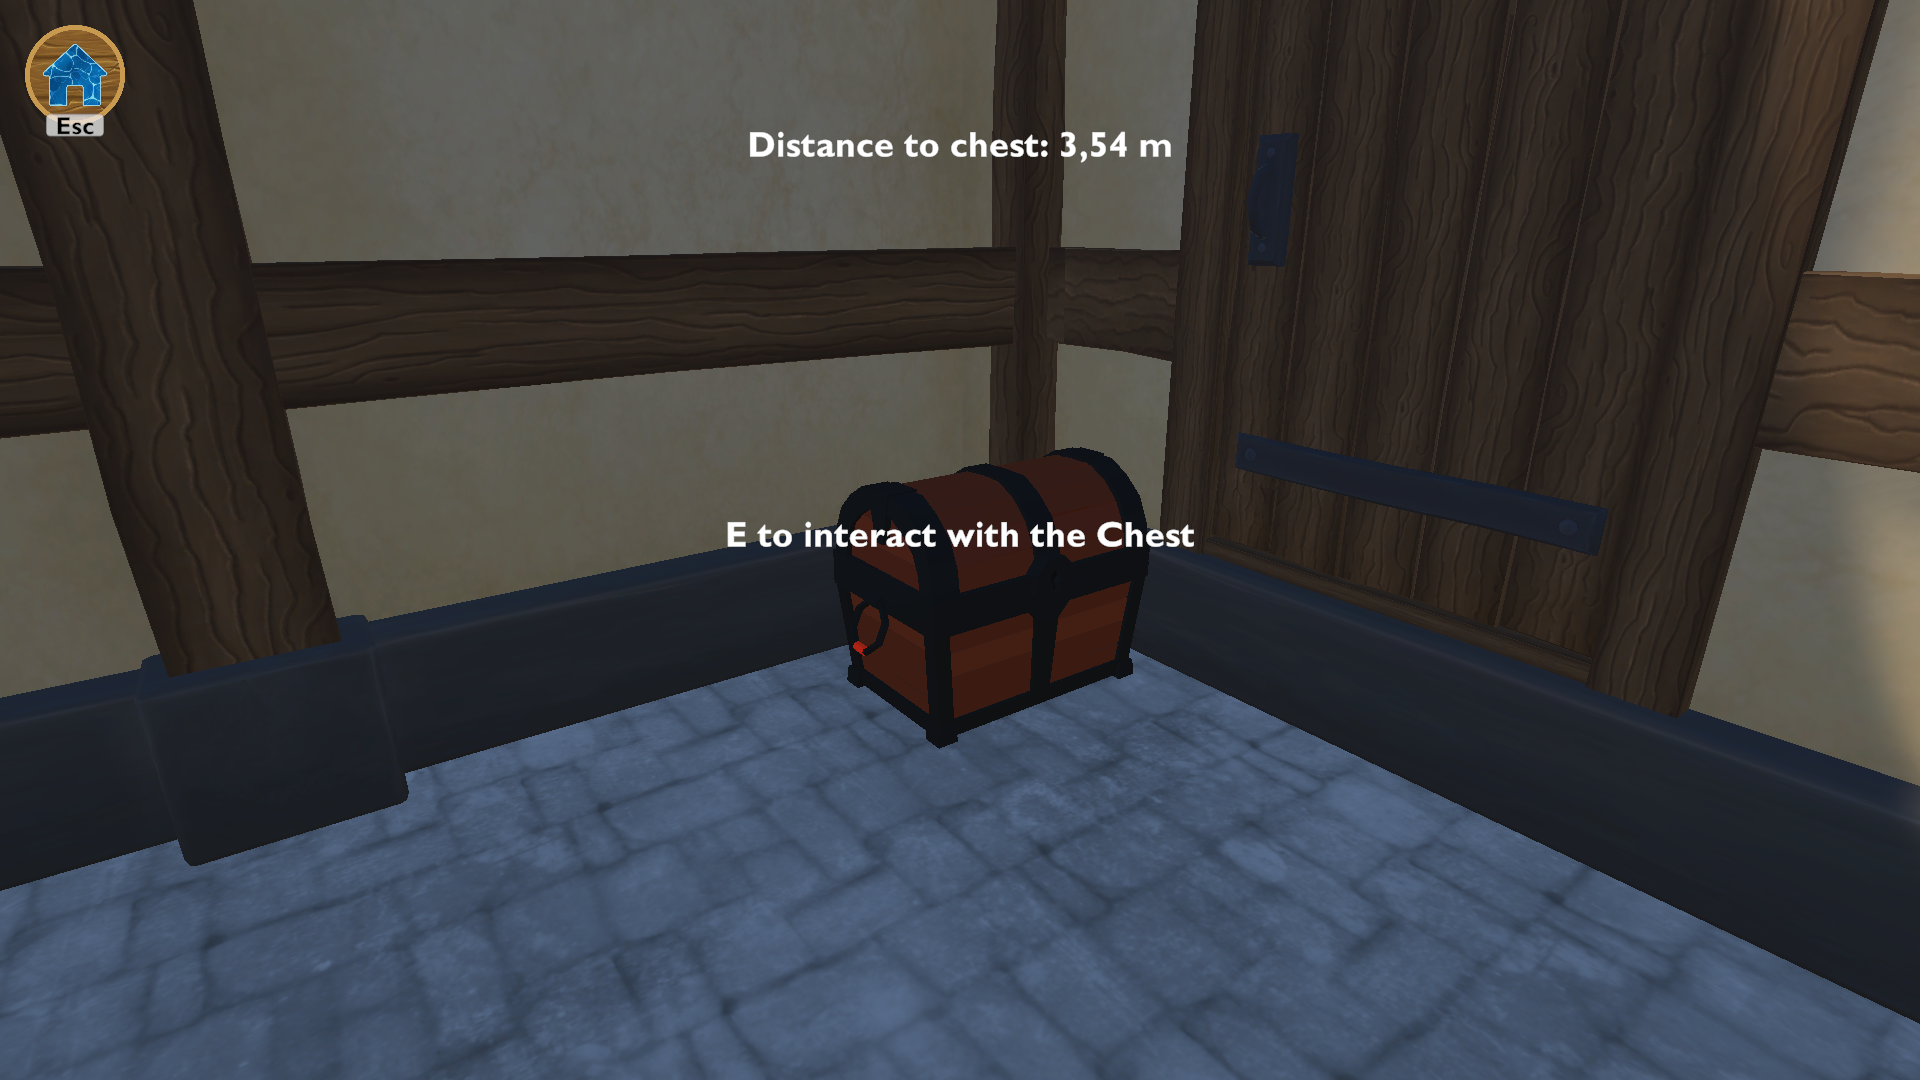
\includegraphics[width=4in]{Illustration/Multiplayer/TreasureHunt.png}
\end{center}

The boat race mini-game begins with each player being teleported to the pier, where their boats await. Once boarded, the objective is to sail across the map, guided by a series of buoys that mark the path to the final destination. Interaction with the final buoy determines the winner. Similar to the treasure hunt, an appropriate user interface screen is triggered at the conclusion of the race based on whether a player wins or loses.\\

\begin{center}
    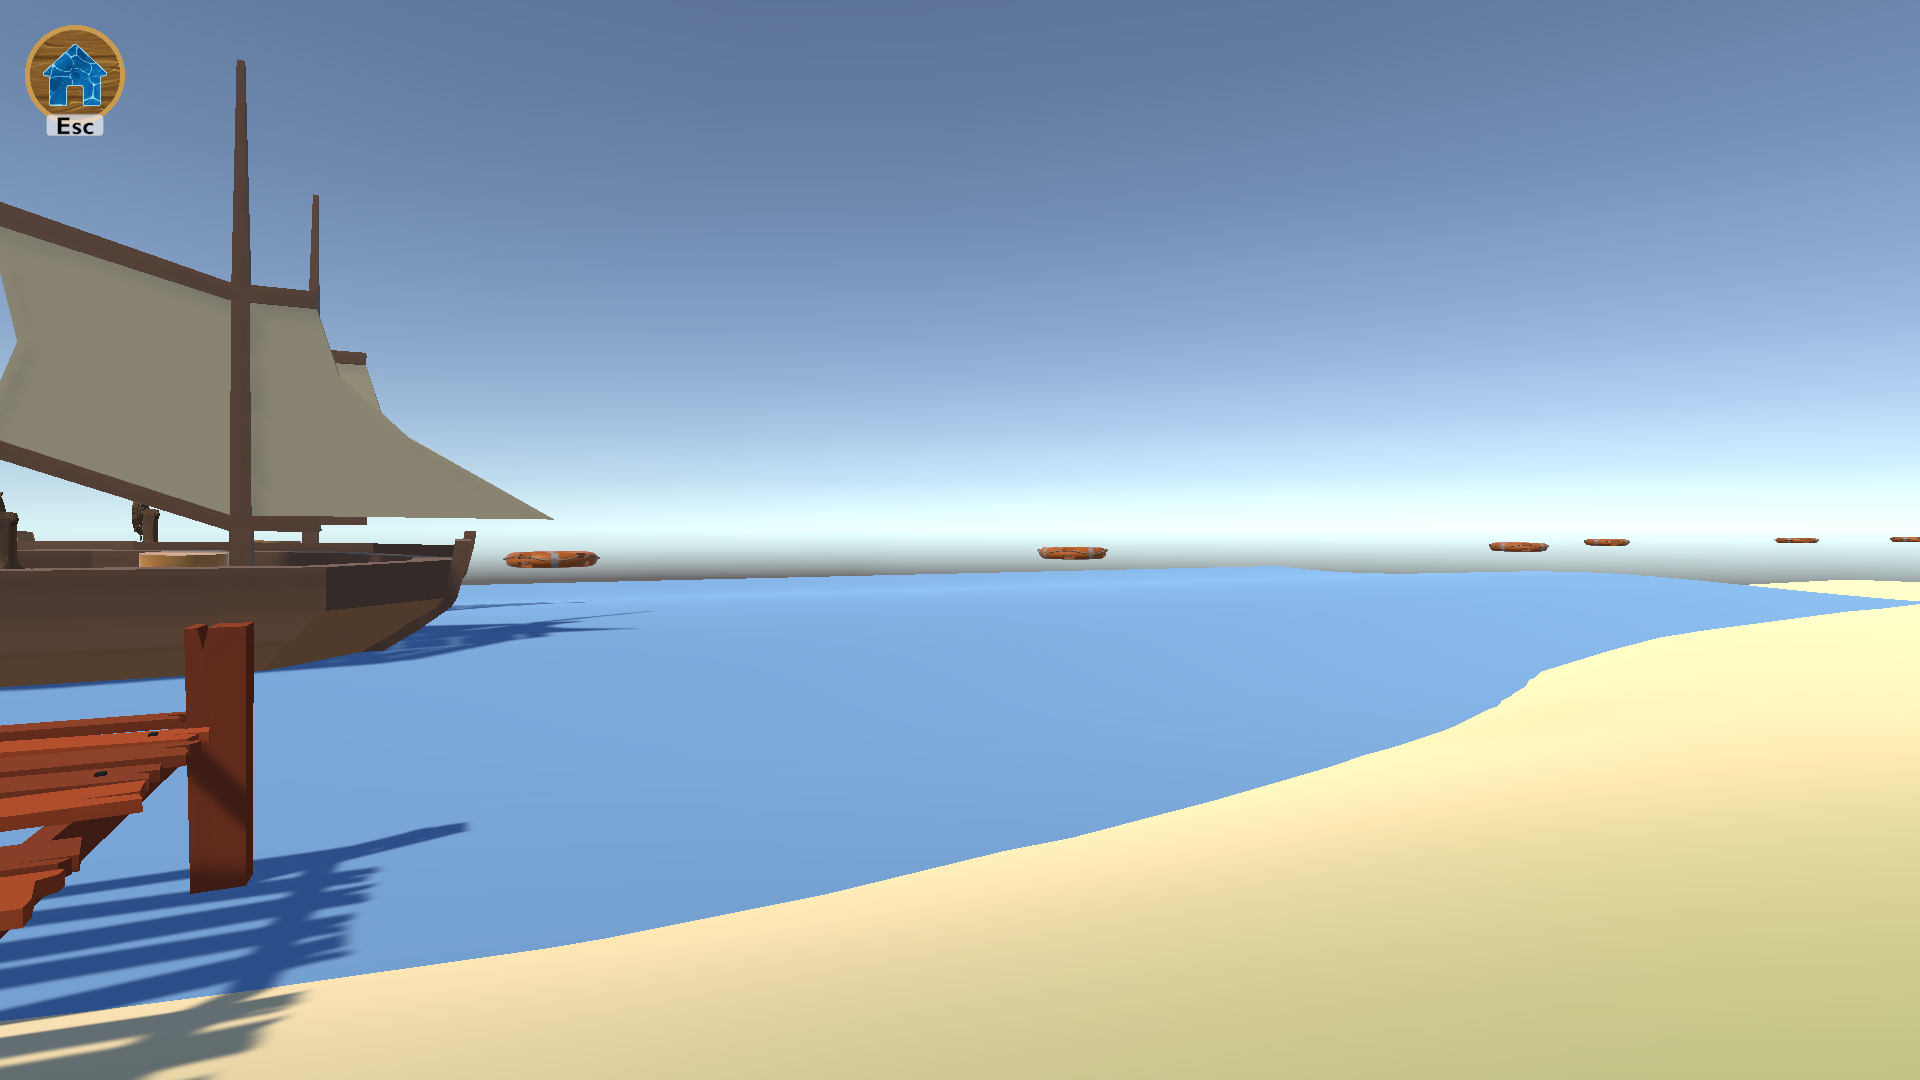
\includegraphics[width=4in]{Illustration/Multiplayer/BoatRace.png}
\end{center}

\begin{center}
    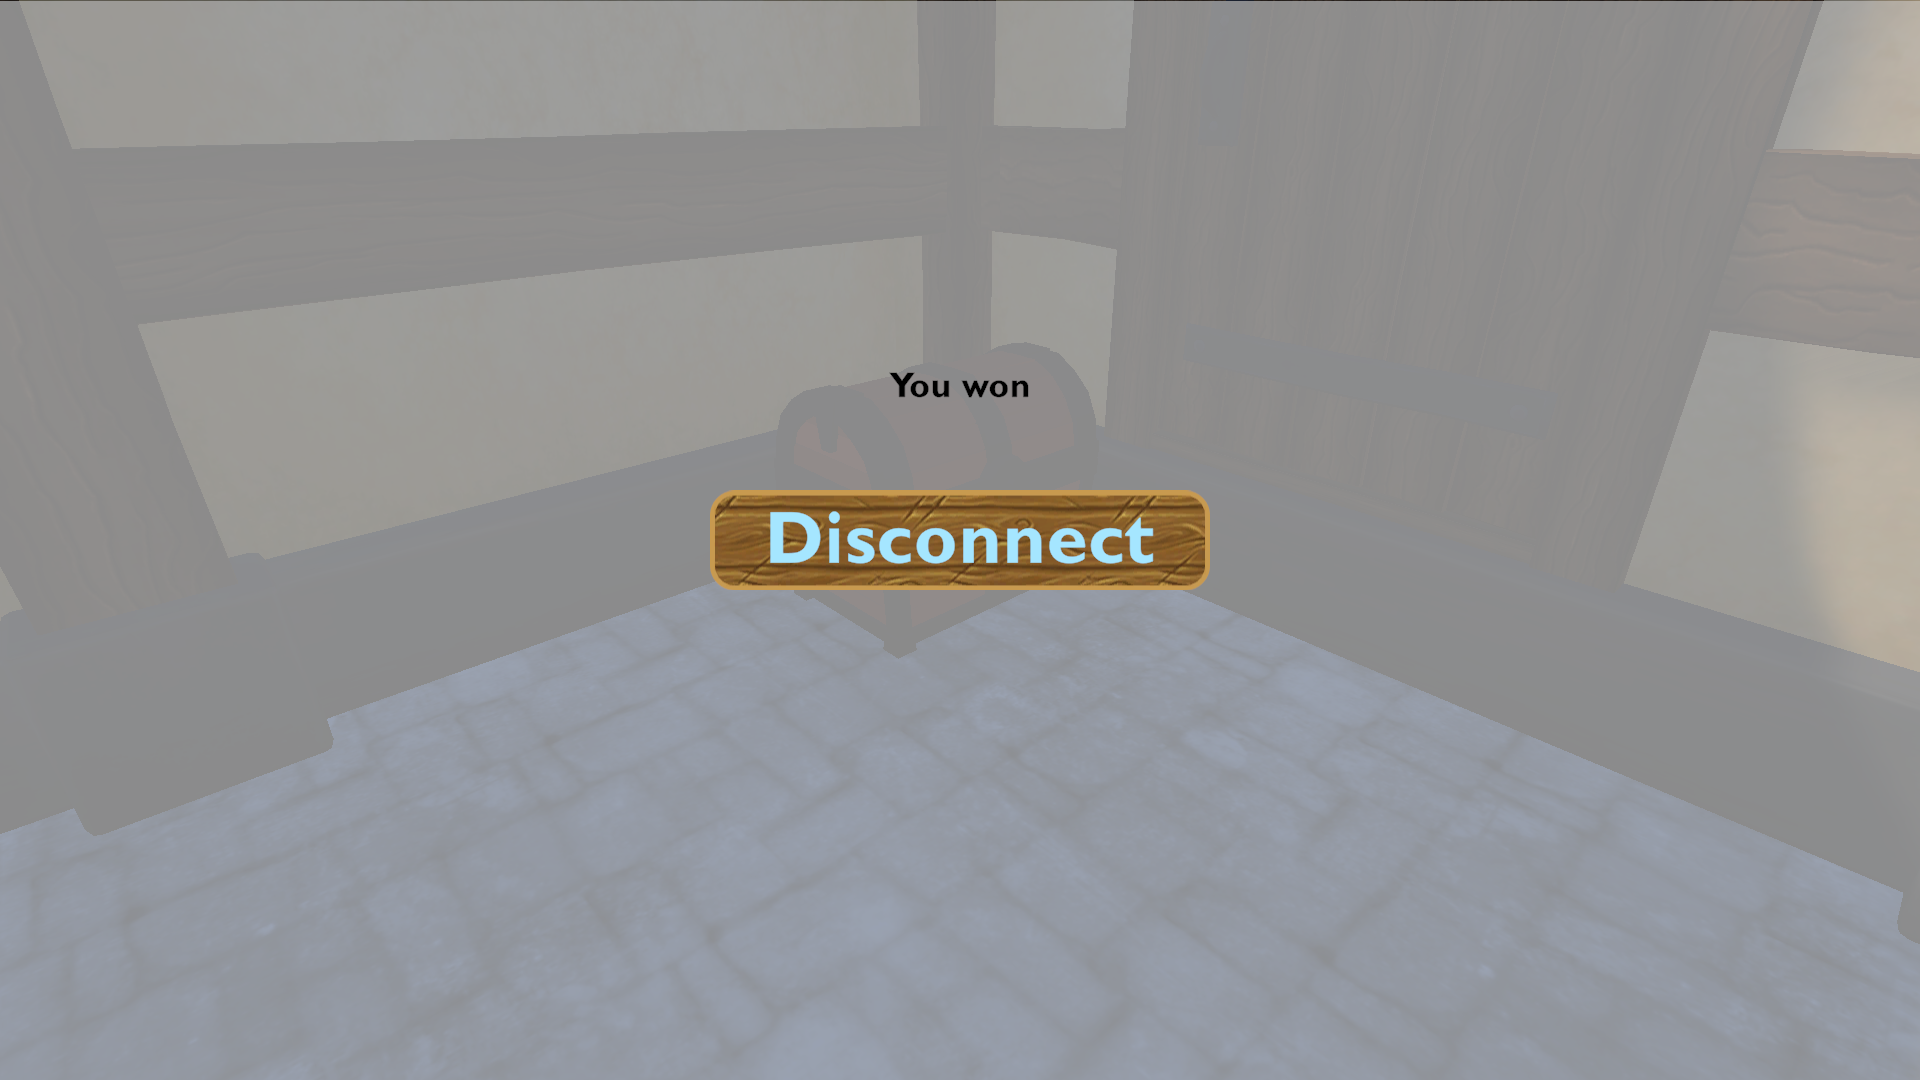
\includegraphics[width=4in]{Illustration/Multiplayer/MultiplayerResultMenu.png}
\end{center}    

Robust session management was crucial to maintaining a stable multiplayer experience. A disconnect menu was made accessible at any time during gameplay, allowing players to leave a session manually. Special attention was given to the case of a host disconnecting; in such instances, the system was configured to automatically disconnect all clients to avoid unexpected behavior or lingering network objects.

\paragraph{Results}\hfill

The integration of multiplayer mini-games brought a dynamic new layer to the gameplay experience. These modes provided engaging activities that both complemented the main game and stood on their own as sources of enjoyment. The treasure hunt introduced a playful competition grounded in exploration, rewarding players for their awareness and mobility. The boat race, on the other hand, emphasized skillful navigation and route planning, offering a fast-paced challenge that felt authentic to the game's nautical theme.\\

The technical implementation proved successful, with players able to connect, wait in a shared space, and transition into gameplay smoothly. The use of RPCs ensured that teleportation and object spawning occurred without authority errors, and the user interface effectively communicated progress and outcomes to all participants. Crucially, the system remained stable even under edge cases such as sudden host disconnection.\\

Overall, the multiplayer component enriched the game world by adding meaningful social interaction and a fresh source of replayability. It maintained alignment with the game's aesthetic and lore, while providing players with exciting, interactive ways to connect and compete.










\newpage
\subsection{Story}
\paragraph{Objective}\hfill

The goal was to create a well-crafted narrative that would immerse players, strengthen their emotional connection to the world, and provide a clear sense of purpose. By establishing a compelling backstory and thematic consistency, the narrative aimed to support player engagement and long-term retention while enhancing the game's adventurous and historical atmosphere.

\paragraph{Implementation}\hfill

The foundation of the game's narrative was built around a richly developed origin story for the main character. The protagonist is portrayed as the son of a merchant who vanished at sea under mysterious circumstances, leaving behind a significant debt to a dominant trading syndicate known as The Merchants of the Shattered Seas.\\

This backstory is revealed through a colonial-era-style letter, written in period-appropriate language and tone. The letter serves as a key lore artifact, offering players an emotional and contextual starting point for their journey.\\

To reinforce the game's tone and historical theme, the opening screen presents a stylized maritime quote: “It's not the man who takes the seas, it's the seas that take the man.”\\

This line subtly references well-known seafaring tropes, providing thematic depth while also adding a touch of humor for those who recognize the homage.\\

Narrative elements were further embedded into the game through environmental storytelling and design cues, ensuring the story is not just told, but felt—through locations, item descriptions, and character interactions that consistently reflect the core themes of loss, legacy, and exploration.

\paragraph{Result}\hfill

The integration of a strong narrative foundation successfully deepened player immersion and emotional investment in the game world. The origin story, delivered through a historically styled letter, created an immediate sense of mystery and motivation.\\

Combined with thematic elements like the opening quote and environmental storytelling, the narrative provided players with a purpose-driven experience. This approach enriched the gameplay, promoted long-term engagement, and helped establish a distinctive and memorable identity for the game.









\newpage
\subsection{Quest}
\paragraph{Objective}\hfill

The primary goal of the quest system was to deliver a simple yet engaging narrative experience that would guide the player through the game's overarching storyline. Rather than relying on complex mechanics or branching decision trees, the system focuses on story-driven progression, centered around interactions with Quest NPCs. These interactions introduce players to the tale of the old merchant's son, forming the backbone of the narrative as players travel from island to island.

\paragraph{Implementation}\hfill

The quest system was built around Unity's raycasting technology to enable direct and intuitive player-NPC interaction. When a player faces a Quest NPC and presses the ‘E' key, a ray is projected from the character's viewpoint to detect any interactable object within a certain range. If a Quest NPC is within reach and line of sight, the interaction is triggered.\\

\begin{center}
    
\includegraphics[width=4in]{Illustration/Quest/NPC.png}
\end{center}

Upon activation, the system begins displaying a series of dialog messages specific to the current island. These dialogs are drawn from a JSON file, where each of the game's nine islands has a predefined set of dialog entries. Each message is shown for a fixed duration of 10 seconds before seamlessly transitioning to the next, allowing the player to absorb the story without requiring manual input or causing gameplay interruption.\\

\begin{center}
    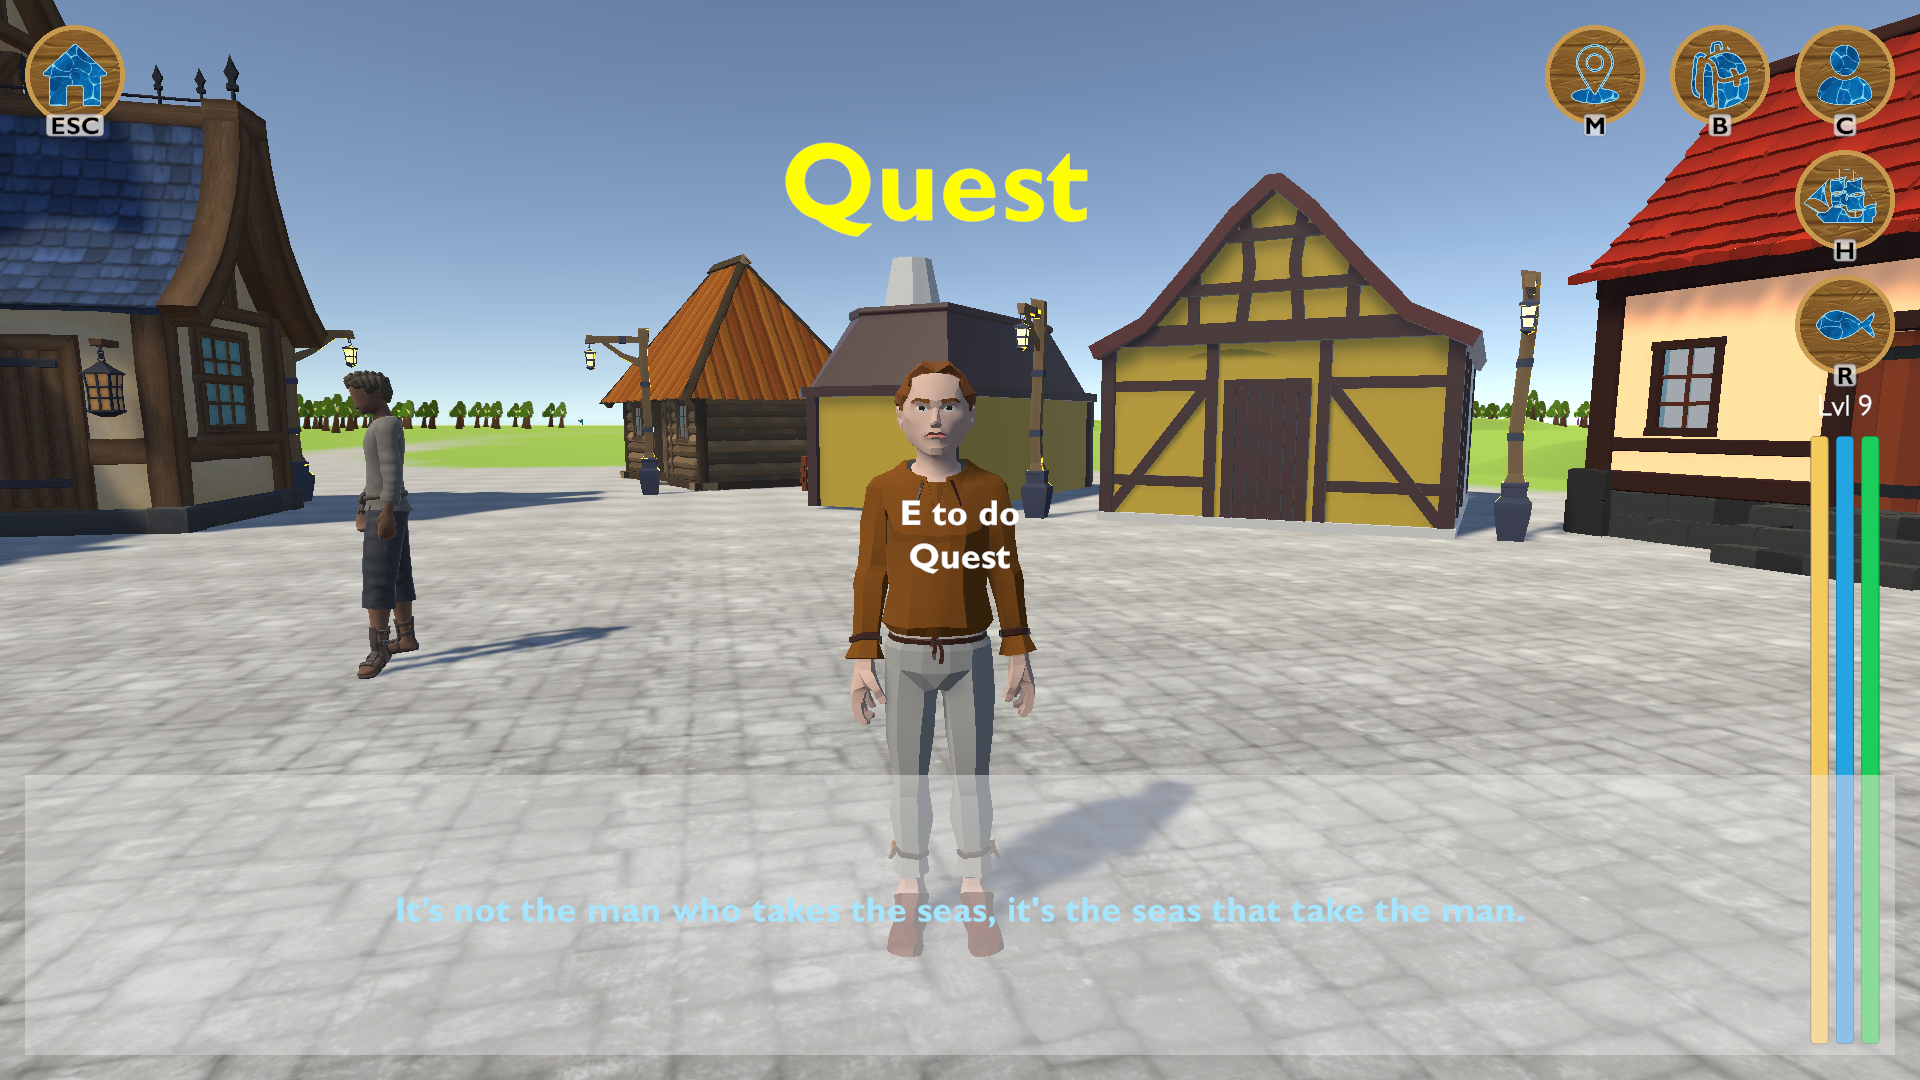
\includegraphics[width=5in]{Illustration/Quest/Dialogs.png}
\end{center}

These dialogs are rendered through Unity's UI system and follow the visual style established for the game, ensuring that the storytelling remains clear and aesthetically consistent. Once the system for interaction and dialog sequencing was completed, Quest NPCs were strategically placed in the central town markets of each island. This placement ensures they are both easy to find and naturally encountered as part of the player's exploration.

\paragraph{Result}\hfill

The completed quest system provides a cohesive and immersive narrative experience without overcomplicating the gameplay. The use of raycasting allows for precise and intuitive interaction, while dialog management through external JSON files ensures scalability and easy maintenance. Strategic placement of Quest NPCs in town centers makes it simple for players to engage with the storyline as they progress through each island. Altogether, the system supports a smooth narrative flow, tying together exploration, interaction, and storytelling in a streamlined and accessible manner.









\newpage
\subsection{Web Site}
\paragraph{Objective}\hfill

The project began with the goal of creating a well-structured and user-friendly website tailored to meet specific project requirements. An essential early step was designing the general layout and framework of the site, establishing a clear vision for its structure and key pages to ensure it aligned with the intended purpose and user expectations.

\paragraph{Implementation}\hfill

Following the initial planning, a market study was conducted to analyze the practices of various video game development companies. This research provided valuable inspiration and helped guide the project to align with industry standards.\\

Technical development kicked off with writing core HTML and CSS code, defining the website's visual style and structural elements. This hands-on coding phase transformed conceptual designs into tangible components, marking significant progress.\\

As the project progressed, attention turned to planning the deployment strategy. After thorough evaluation, the decision was made to adopt Odoo, a powerful platform known for its integration and management capabilities. While this strategic pivot offered long-term benefits such as scalability and efficiency, it also required resetting several configurations and restarting parts of the work. This setback posed challenges but ultimately contributed to a stronger foundation for the project.\\

In the final phase, all remaining aspects—including graphic design, technical features, and functional components—were carefully refined and completed. This comprehensive effort ensured the website not only fulfilled the initial goals but also delivered a polished and professional user experience.

\paragraph{Result}\hfill

The project culminated with the successful deployment of the website, marking the completion of an intensive development phase. Despite setbacks and technical hurdles, the website was launched with a coherent structure, visually appealing design, and reliable functionality. This milestone represented a major achievement, setting the stage for future developments and expanding the project's overall scope.










\newpage
\subsection{Design Entities}
\paragraph{Objective}\hfill

The primary objective was to resolve a visual issue in the first-person camera system where players could see unintended parts of their own character model, such as legs and internal geometry. This broke immersion and disrupted the intended gameplay experience. The goal was to make the player's character invisible from their own camera while ensuring the model remained fully visible to other players in a multiplayer environment. Addressing this was essential for maintaining visual realism and consistency.\\

The objectfive was to find humanoid entities to implement them in the game for the player—the passive and offensive NPCs including terrestrial and maritime enemies. Some entities were found on \url{https://poly.pizza} and others were found on Unity's Asset Store, especially for the passive NPCs, which is very useful for the diversity of NPCs in the village. And on Unity's Asset Store libraries, we are sure to have the 3D model rigged, which was very practical for the animation.

\paragraph{Implementation}\hfill

The issue stemmed from the visibility of the character model's internal textures when viewed from a first-person perspective. Initial efforts to resolve the problem by adjusting the Mesh Renderer directly in Unity were blocked, as the Mesh Renderer component was not exposed in the Inspector for the current model. To work around this limitation, a duplicate of the player model was created—one with a visible and accessible Mesh Renderer—enabling full material control.\\

To ensure visual consistency, the original albedo texture (color texture) was extracted from the .fbx model using Blender. A publicly available tutorial guided the texture extraction process (\url{https://youtu.be/wG6ON8wZYLc}), ensuring it was cleanly exported as a .png file suitable for Unity.\\

\begin{center}
    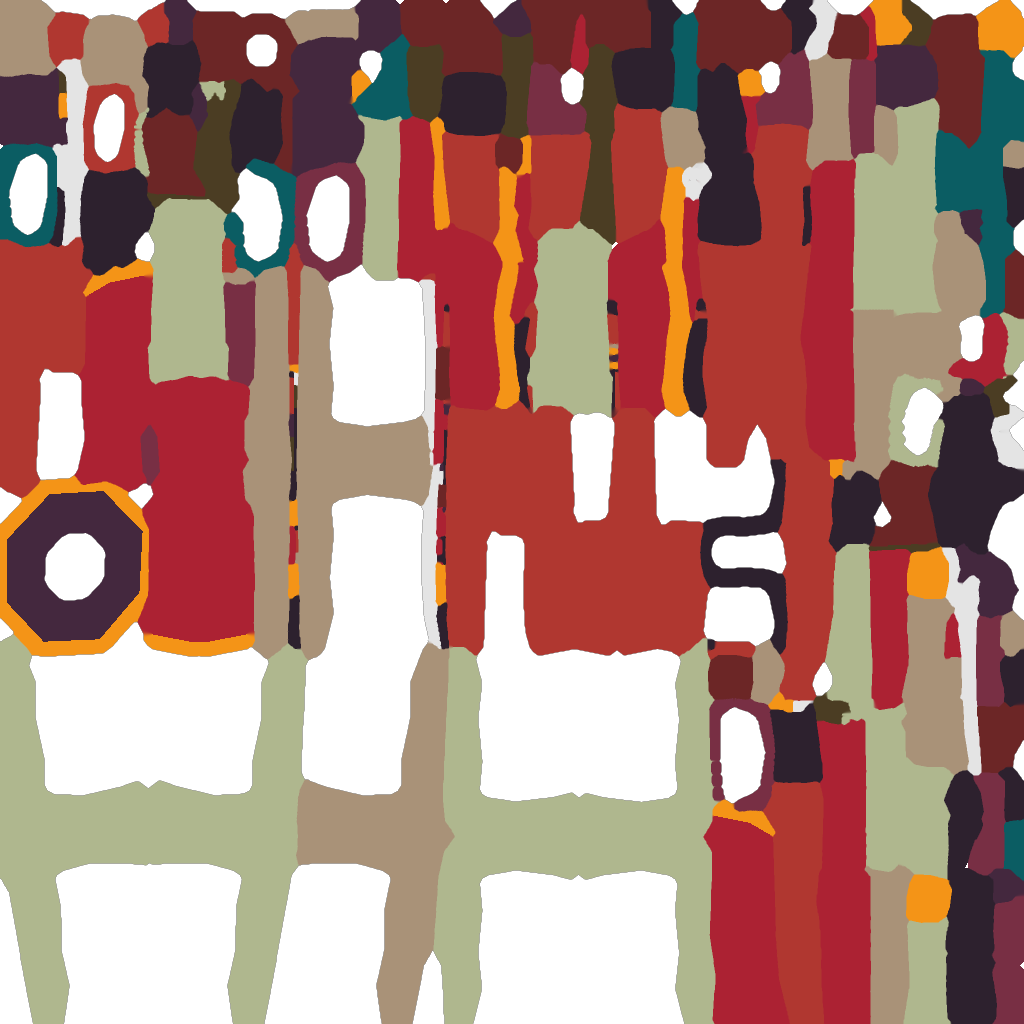
\includegraphics[width=2in]{Illustration/3DModel/Pirate1.png}
\end{center}

Once extracted, the texture was applied to the duplicate model in Unity.\\

\begin{center}
    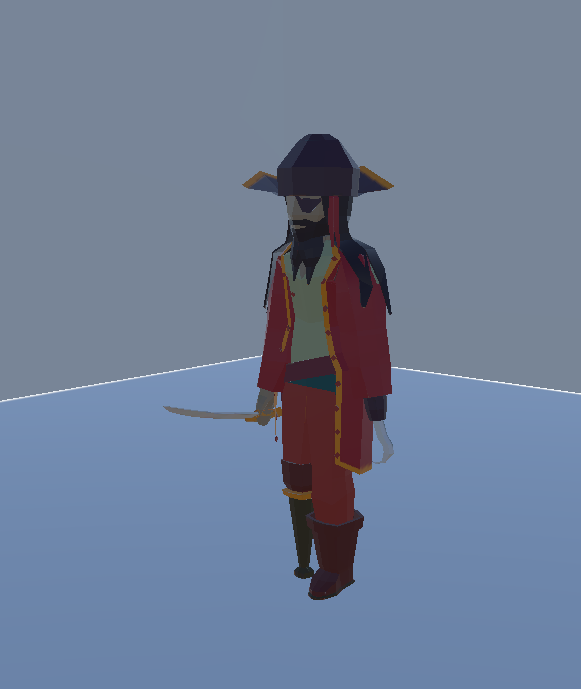
\includegraphics[width=2in]{Illustration/3DModel/Pirat.png}
\end{center}

During the animation testing phase, it was observed that the player's own texture, including elements such as the leg, was visible through the first-person camera. This visibility of the internal texture created an unrealistic and immersion-breaking effect. The core issue was that the player could see the inside of the 3D model's texture from their own perspective. The objective was to develop a solution that would hide the player's texture exclusively from their own camera view, while maintaining full visibility of the player's model for other participants in a multiplayer environment. Addressing this was critical to preserving immersion and realism during gameplay.\\

One approach involved moving the camera on the player prefab by a very small distance to mitigate the visibility issue.\\

This system allowed seamless control of visibility without affecting the integrity of the multiplayer environment.

\paragraph{Result}\hfill

The final implementation effectively resolved the immersion-breaking issue. By combining Blender-based texture extraction, Unity material management, and a custom scripting system, the local player no longer saw their own character model in first-person mode. The model remained fully visible to other players, preserving multiplayer functionality.\\

The solution significantly enhanced the visual and immersive quality of the gameplay experience. Despite requiring coordination between Blender and Unity and a multi-step process, the result was a robust and scalable system. The project achieved its goal of improving realism without compromising multiplayer integrity.










\newpage
\subsection{Animations of entities}
\paragraph{Objective}\hfill

The key objective was to implement smooth and responsive player animations covering a range of actions such as idle, running, walking, attacking, swimming, and death. This was essential to enhance the visual coherence and realism of the player's movements and integrate seamlessly with the existing movement system, thereby improving overall gameplay immersion.

\paragraph{Implementation}\hfill

The process started with foundational research into animation principles and skeletal rigging, utilizing various tutorials to gain a solid understanding of workflows:
\begin{itemize}
    \item \url{https://youtu.be/2_Hn5ZsUIXM} 
    \item \url{https://youtu.be/vApG8aYD5aI} 
    \item \url{https://youtu.be/s5lRq6-BVcw} 
\end{itemize}

Animations for all required states—idle, running, walking, attacking, swimming, and death—were sourced from Mixamo (\url{https://www.mixamo.com}).\\

Early attempts to apply these animations in Unity revealed the player model lacked a skeleton, preventing proper animation. Attempts to rig the model directly in Unity failed repeatedly. The solution was to rig the player model externally in Blender, guided by a tutorial (\url{https://youtu.be/gdOaUv0_TC8}) which successfully added the necessary bone structure.\\

\begin{center}
    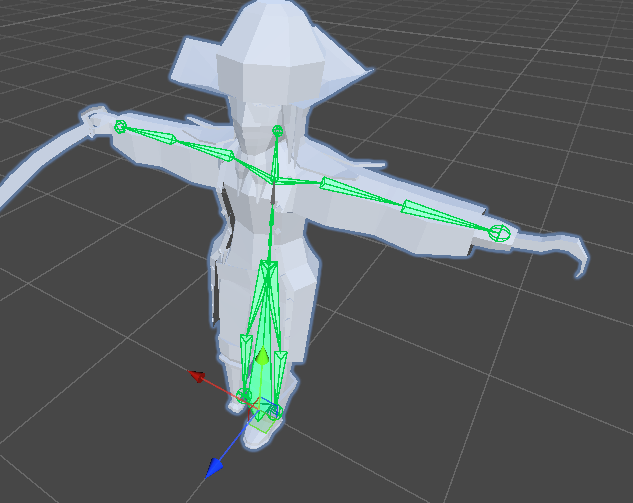
\includegraphics[width=2in]{Illustration/Animation/Rig.png}
    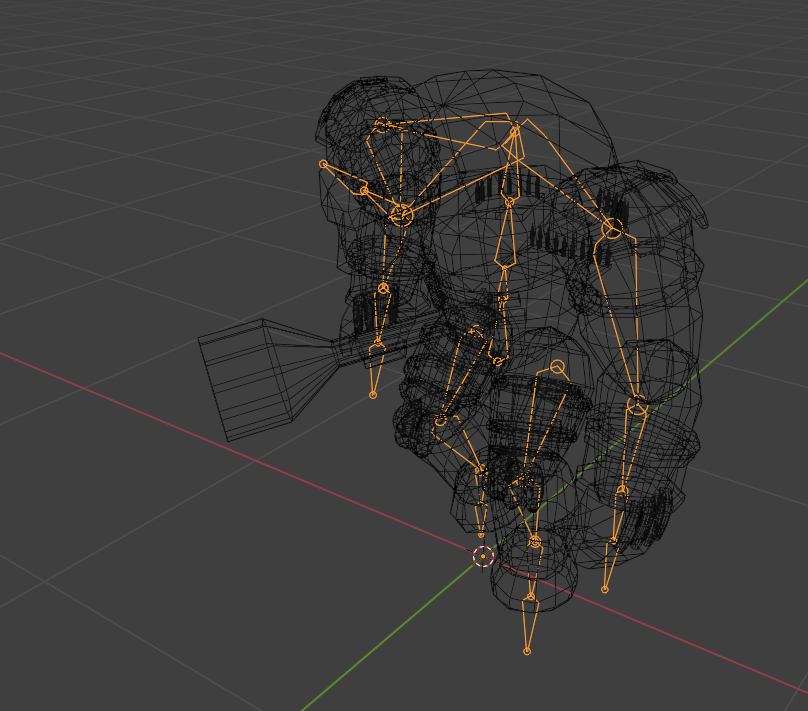
\includegraphics[width=2in]{Illustration/Animation/Rig2.png}
\end{center}

The rigged model was then imported back into Unity, where the Animator Controller was set up to manage the animation states. A custom script was developed to handle smooth transitions between animations based on player input and state changes such as running, attacking, swimming, and jumping.\\

\begin{center}
    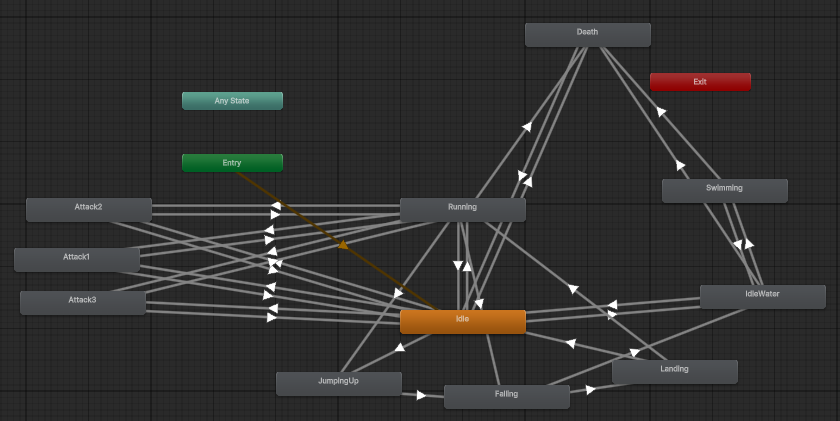
\includegraphics[width=3in]{Illustration/Animation/playeranimator.png}
    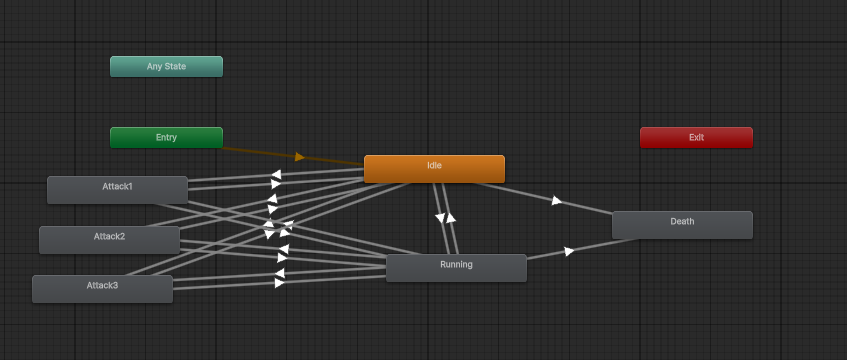
\includegraphics[width=3in]{Illustration/Animation/enemyanimator.png}
\end{center}

Special focus was given to jump and fall animations to make them responsive to varying jump heights and fall distances. This was accomplished with help from a tutorial on dynamic jump and fall behavior (\url{https://youtu.be/sJvWmFYSQFY}), ensuring natural and fluid motion during airborne states.

\paragraph{Result}\hfill

The implementation of a properly rigged player model combined with a fully configured Animator Controller significantly improved the player's visual and gameplay experience. Animations became fluid, context-aware, and responsive to player inputs, resulting in smooth transitions across different movement states.\\

This enhancement brought a new level of polish and immersion to the game, providing more realistic character motion and a dynamic, engaging gameplay environment. The success of this phase laid a strong foundation for future animation improvements and additional character behaviors.










\newpage
\subsection{Music and Sound Effects}
\paragraph{Objective}\hfill

The primary goal was to integrate music and sound effects into the game in a way that enhances player immersion by providing dynamic and responsive audio. This included implementing continuous background music, meaningful sound effects tied to player interactions, and adaptive music transitions that reflect changes in the game environment, thereby enriching the overall gameplay atmosphere.

\paragraph{Implementation}\hfill

All audio assets were sourced as .wav files from the Unity Asset Store and organized within the project for easy management.\\

A dedicated GameObject was created to host two Audio Sources: one dedicated to playing continuous background music, and the other assigned to sound effects like button clicks and interaction cues.\\

\begin{center}
    
\includegraphics[width=3in]{Illustration/MusicSFX/Hiearchy.png}
\end{center}

A custom script was developed to enable the background music to randomly select and play tracks from a specified folder, ensuring auditory variety and maintaining player engagement throughout gameplay.\\

To increase immersion, the system was enhanced to dynamically change the background music based on the player's location within the game world. This involved detecting when players entered specific zones (such as towns or outdoor areas) and smoothly transitioning between different ambient music tracks to better suit the environment.\\

\begin{center}
    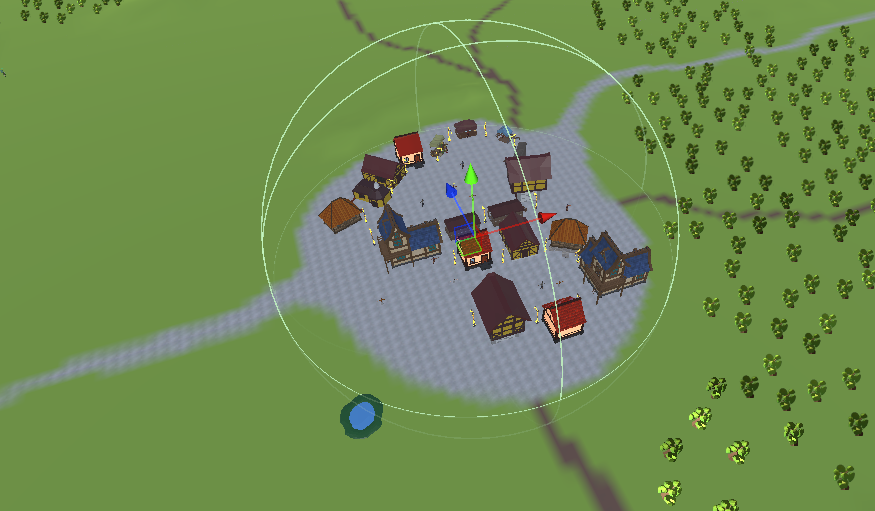
\includegraphics[width=4in]{Illustration/MusicSFX/TownMusicZone.png}
\end{center}

The second Audio Source was configured to trigger sound effects in response to player actions, providing immediate auditory feedback for interactions such as menu navigation and button presses.

\paragraph{Result}\hfill

The implemented audio system significantly enriched the game's auditory experience. Dynamic background music transitions and context-sensitive sound effects created a more engaging, polished, and immersive atmosphere.\\

By adapting the music to different in-game environments and tying sound effects to player inputs, the system deepened the emotional and sensory connection between players and the game world, elevating the overall quality and player experience.




















\newpage
\section*{Appendix}
\subsection*{Menu and User Interface}
\begin{center}
    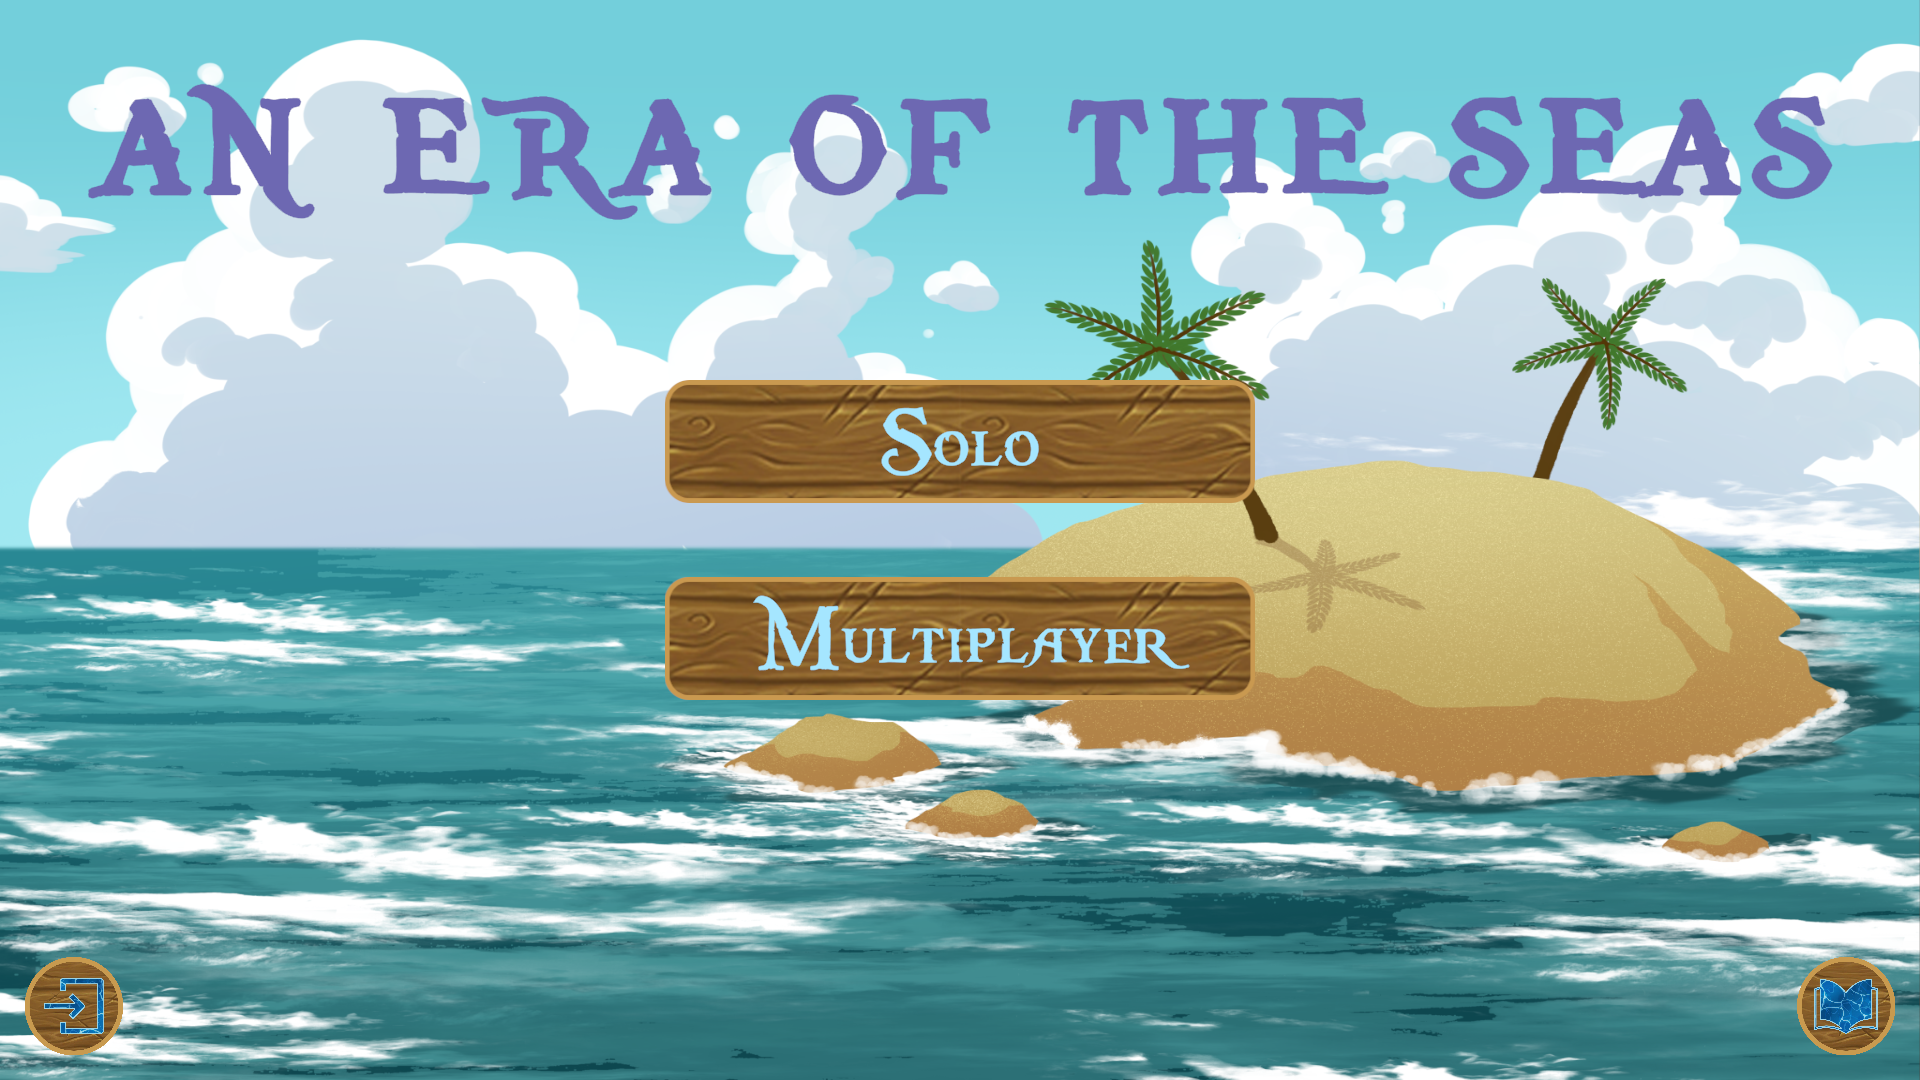
\includegraphics[width=5in]{Illustration/MenuUI/MainMenu.png}
    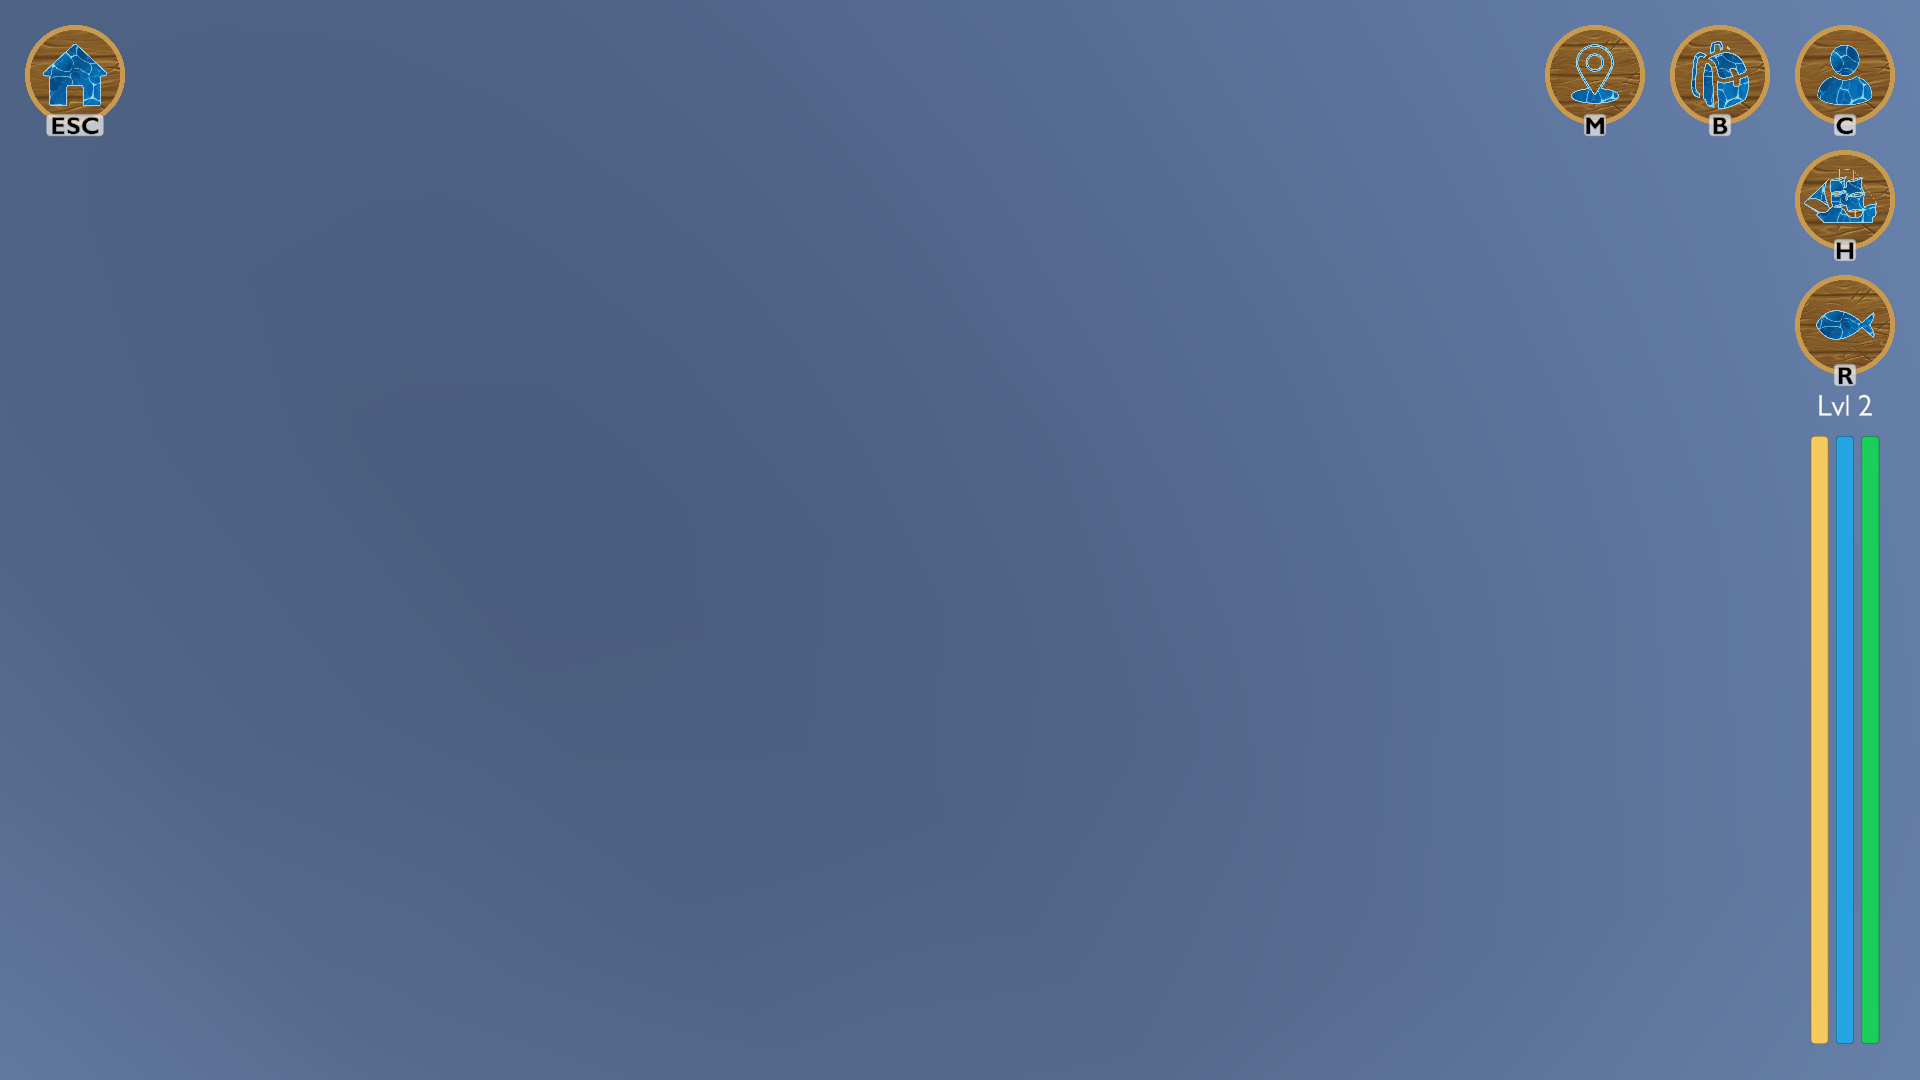
\includegraphics[width=5in]{Illustration/MenuUI/PlayerUI.png}
    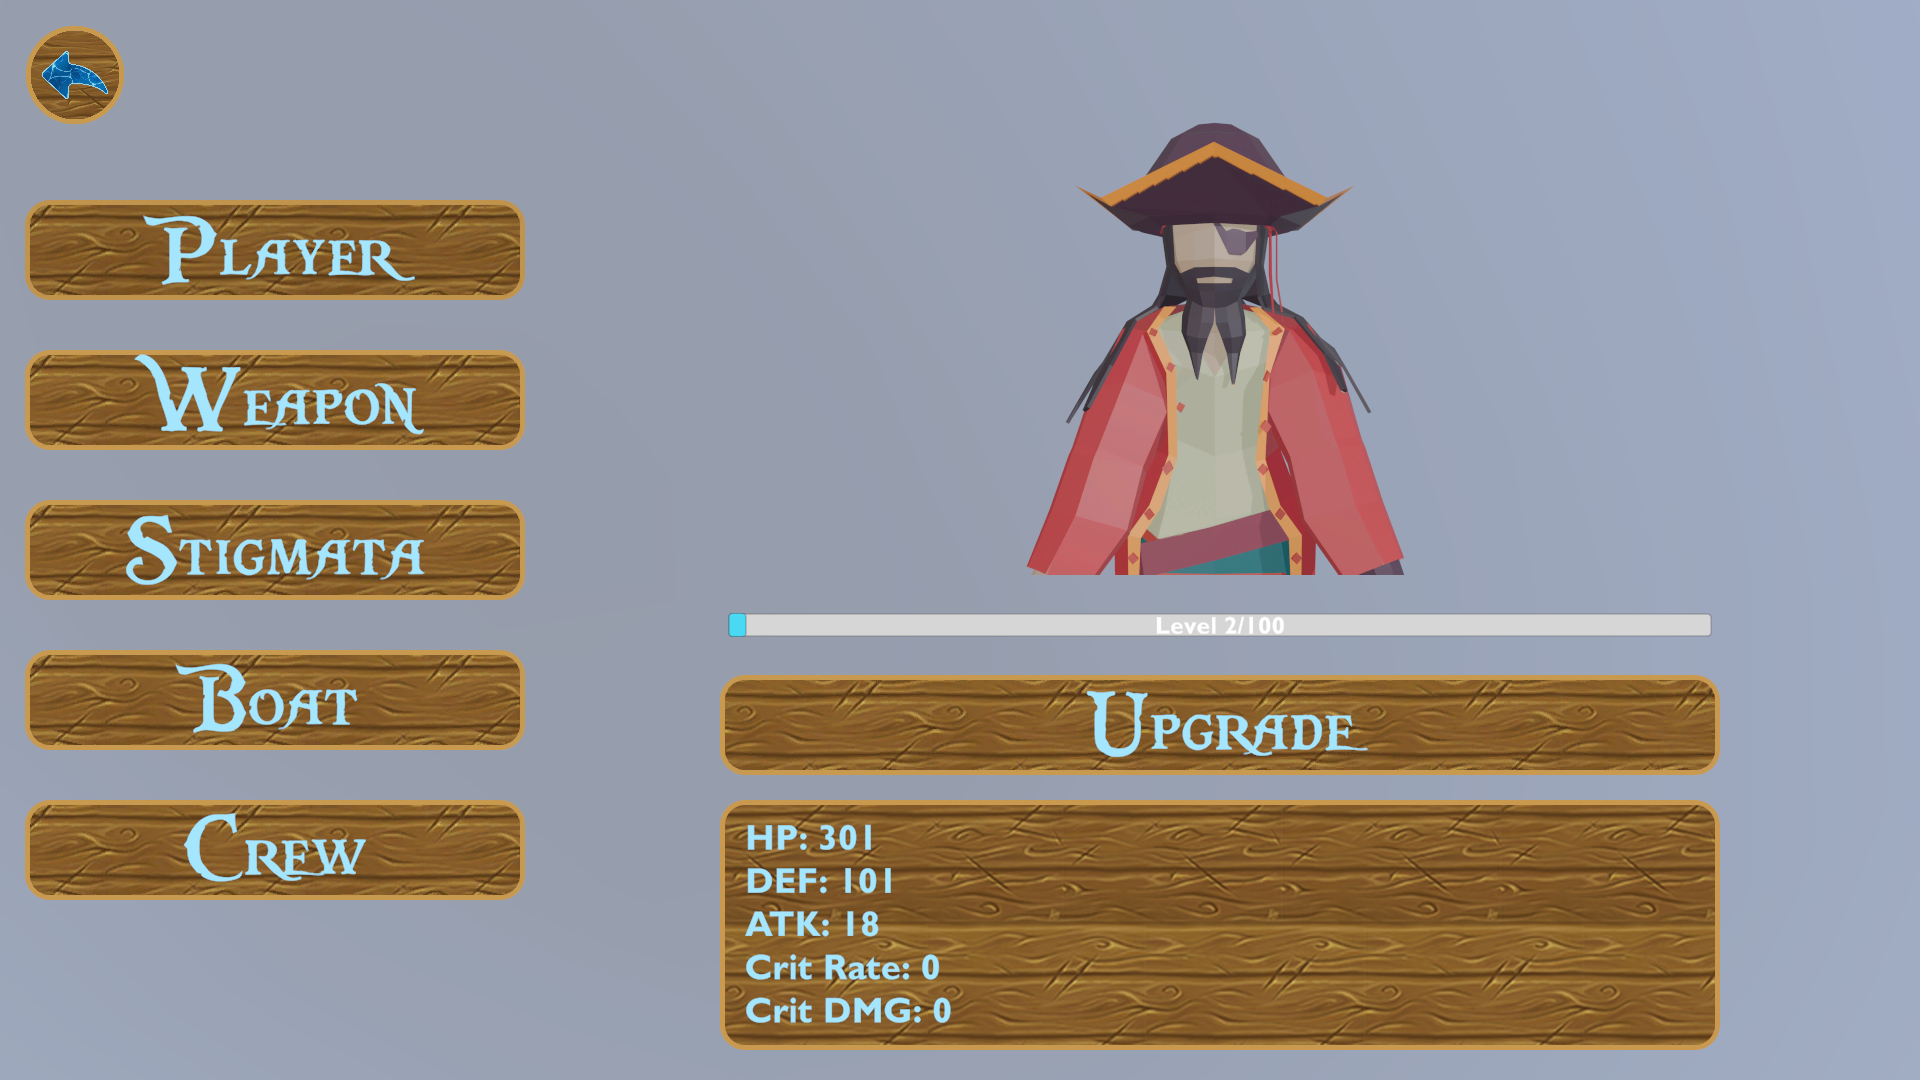
\includegraphics[width=5in]{Illustration/MenuUI/EquipmentMenu.png}
    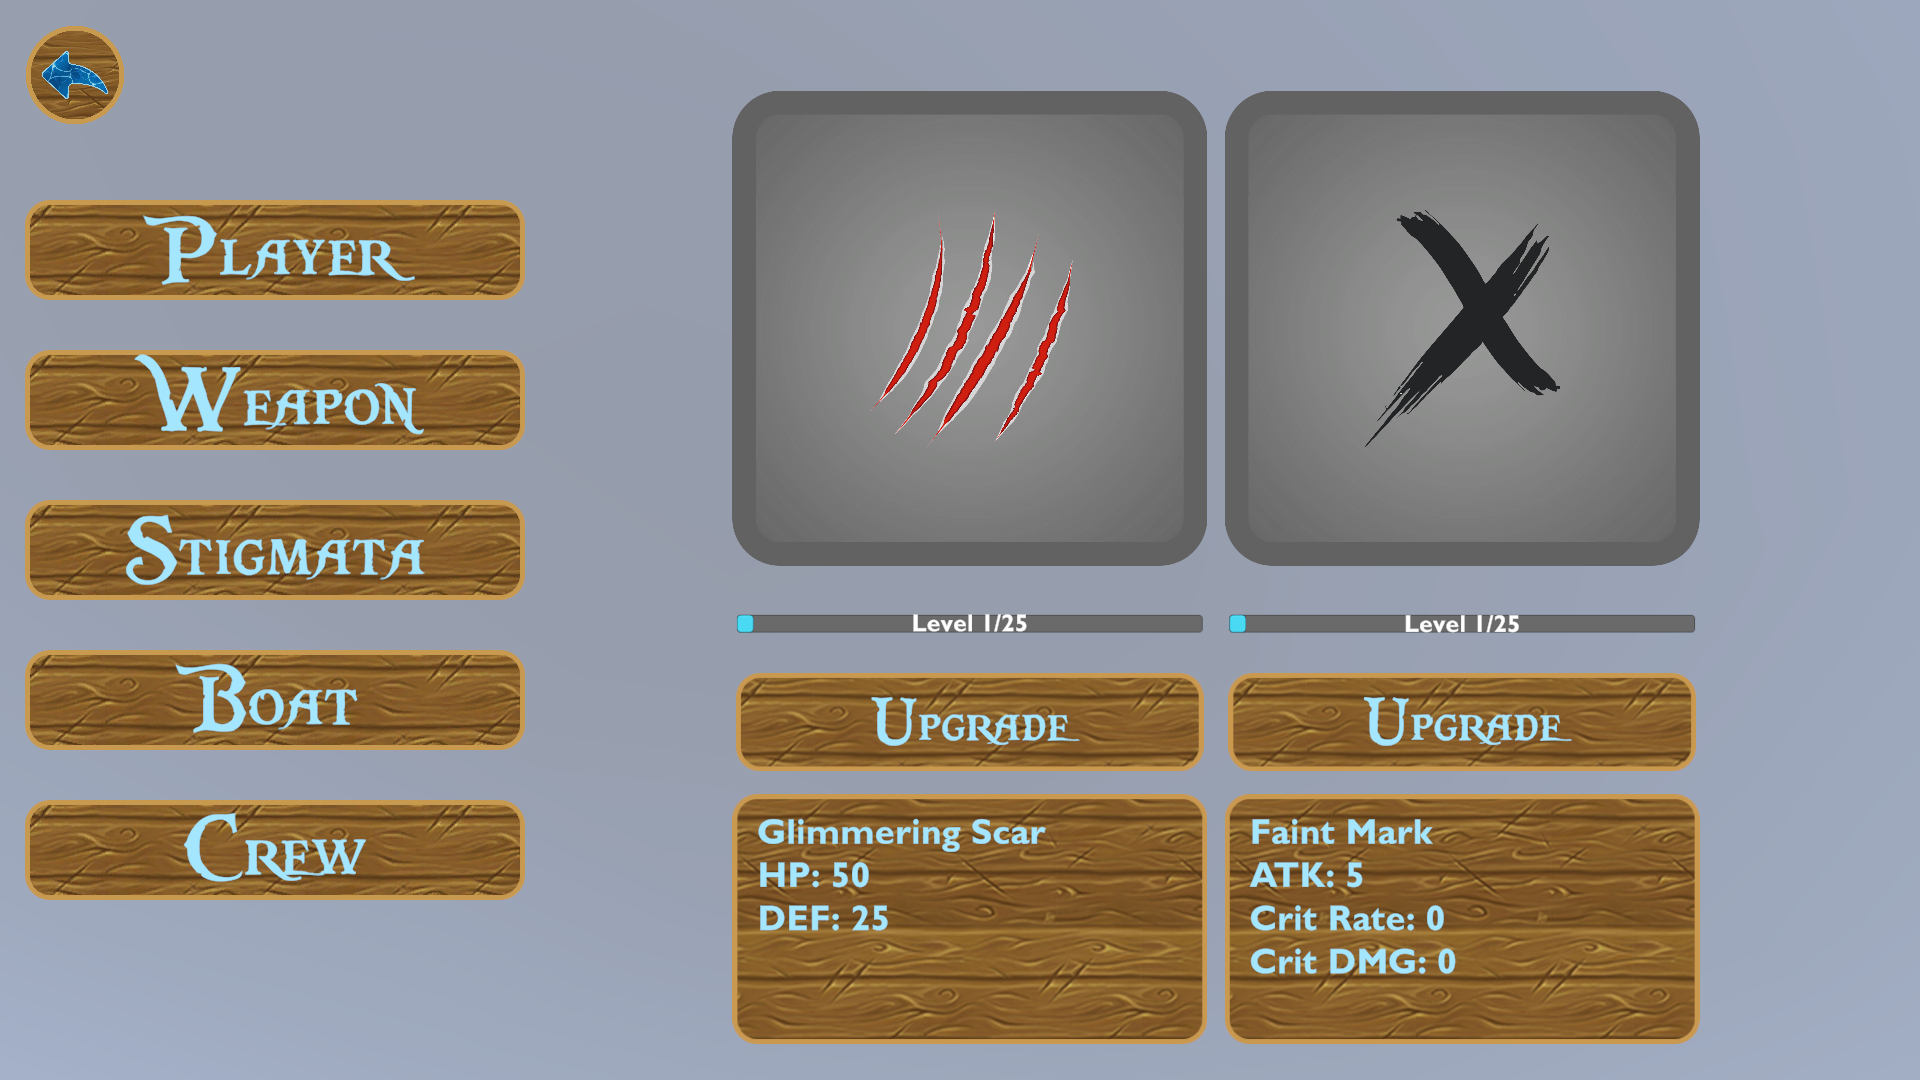
\includegraphics[width=5in]{Illustration/MenuUI/EquipmentMenu2.png}
    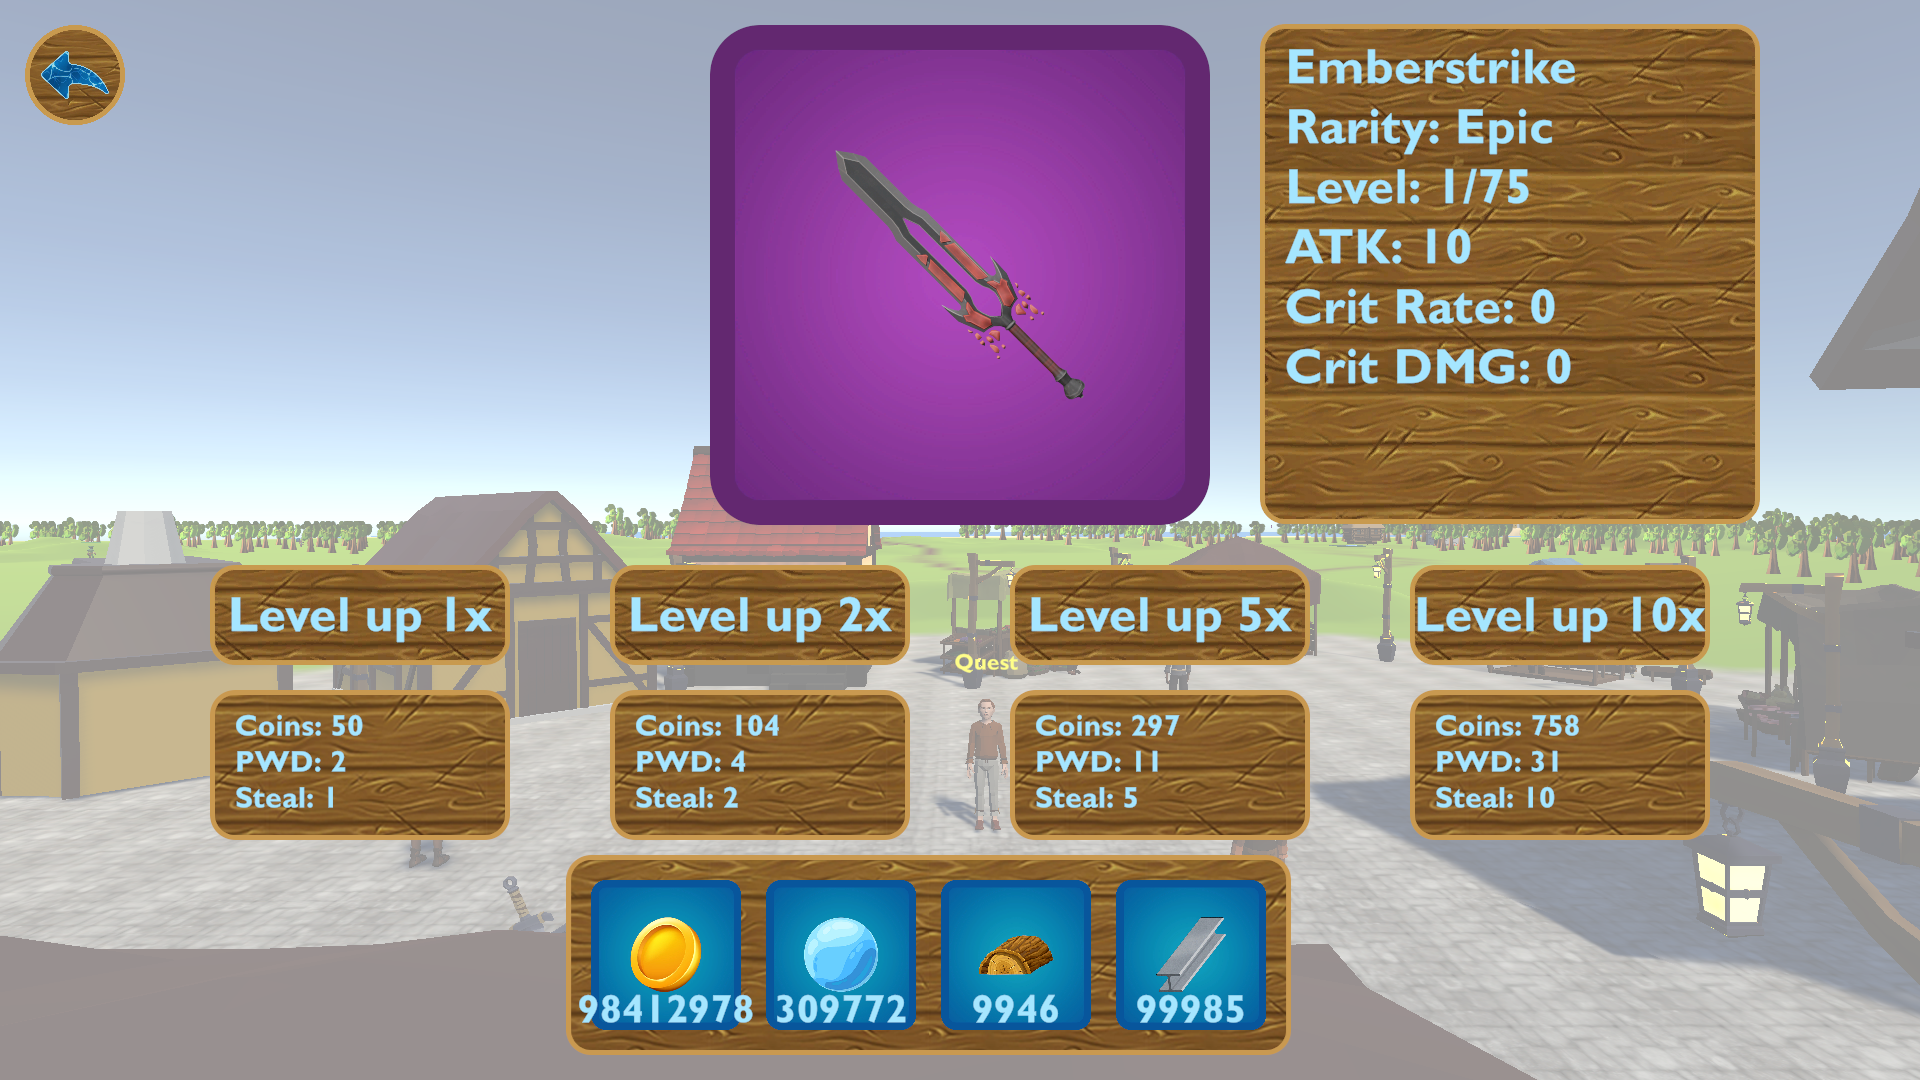
\includegraphics[width=5in]{Illustration/MenuUI/UpgradeMenu.png}
    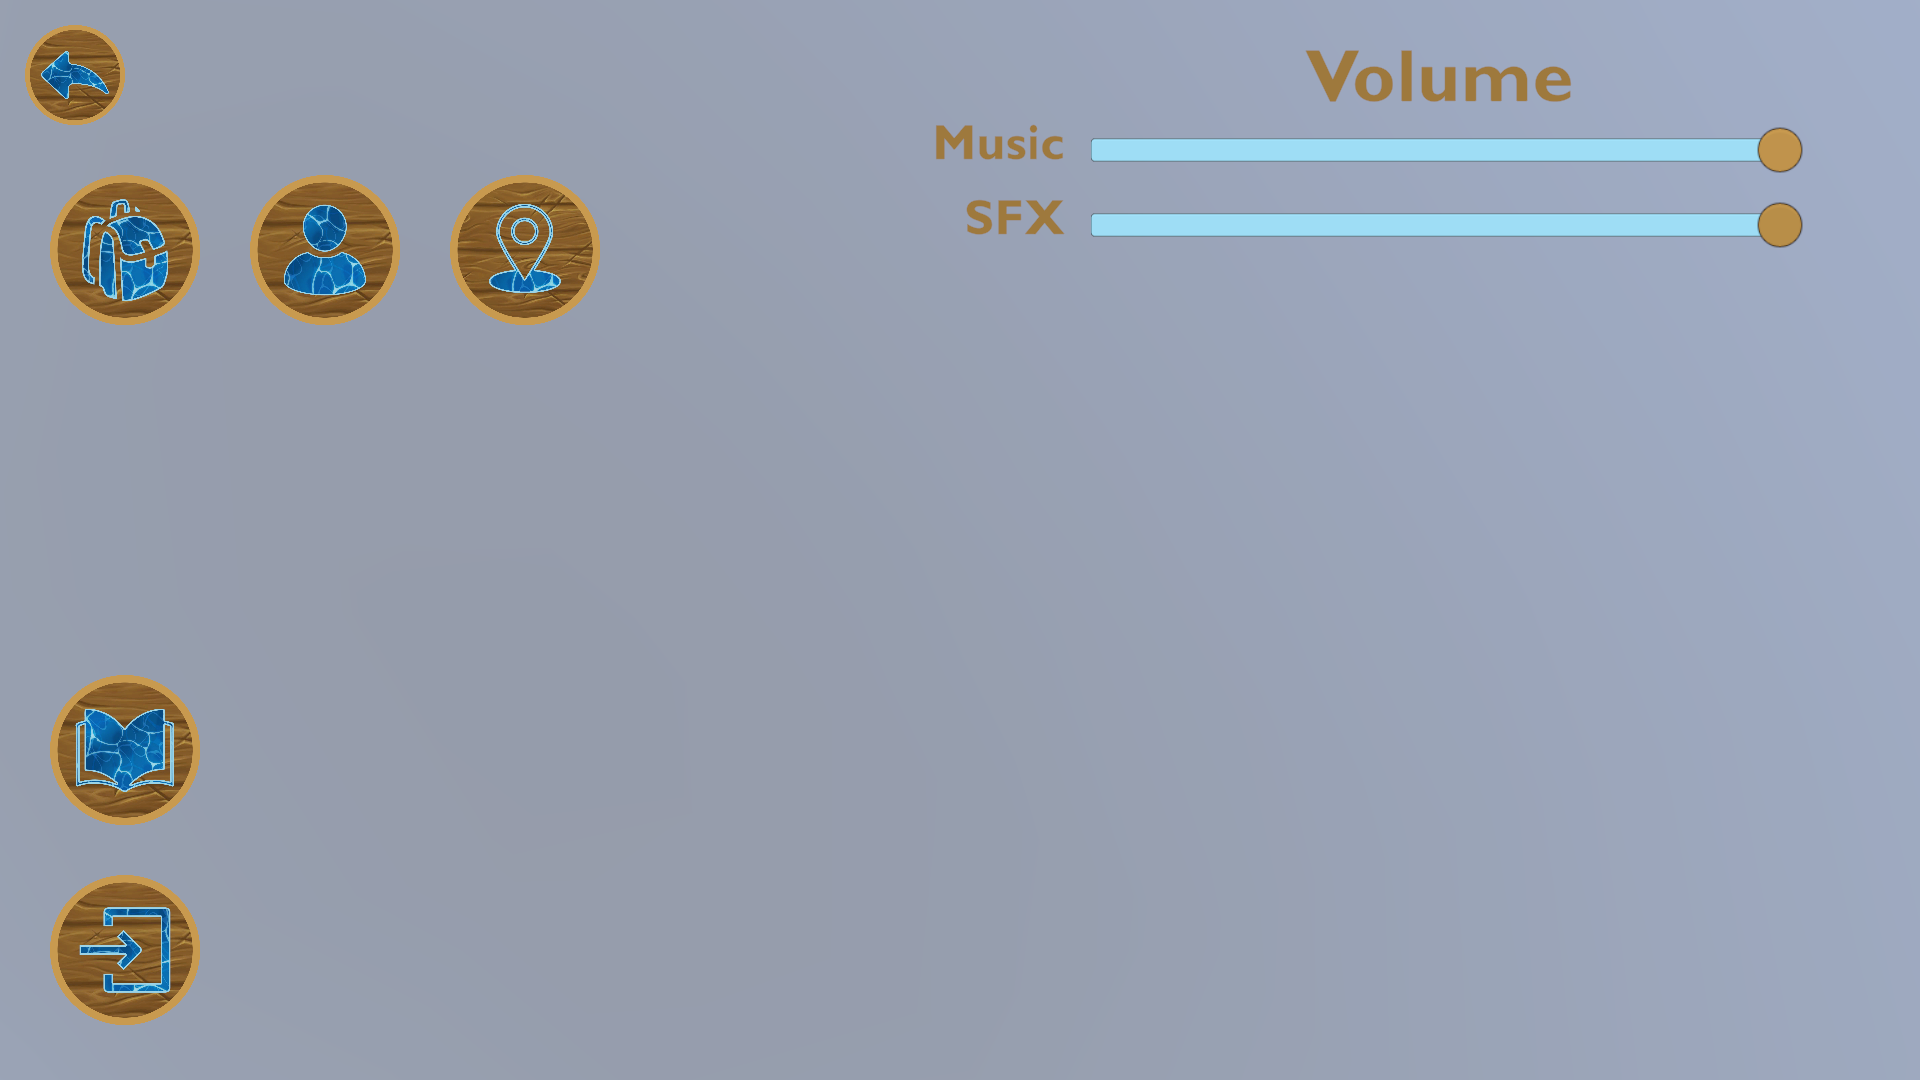
\includegraphics[width=5in]{Illustration/MenuUI/SettingsMenu.png}
    
\includegraphics[width=2in]{Illustration/MenuUI/Button300x100.png}
    
\includegraphics[width=2in]{Illustration/MenuUI/HomeButton.png}
    
\includegraphics[width=2in]{Illustration/MenuUI/ReturnButton.png}
    
\includegraphics[width=2in]{Illustration/MenuUI/QuitButton.png}
    
\includegraphics[width=2in]{Illustration/MenuUI/BackpackButton.png}
    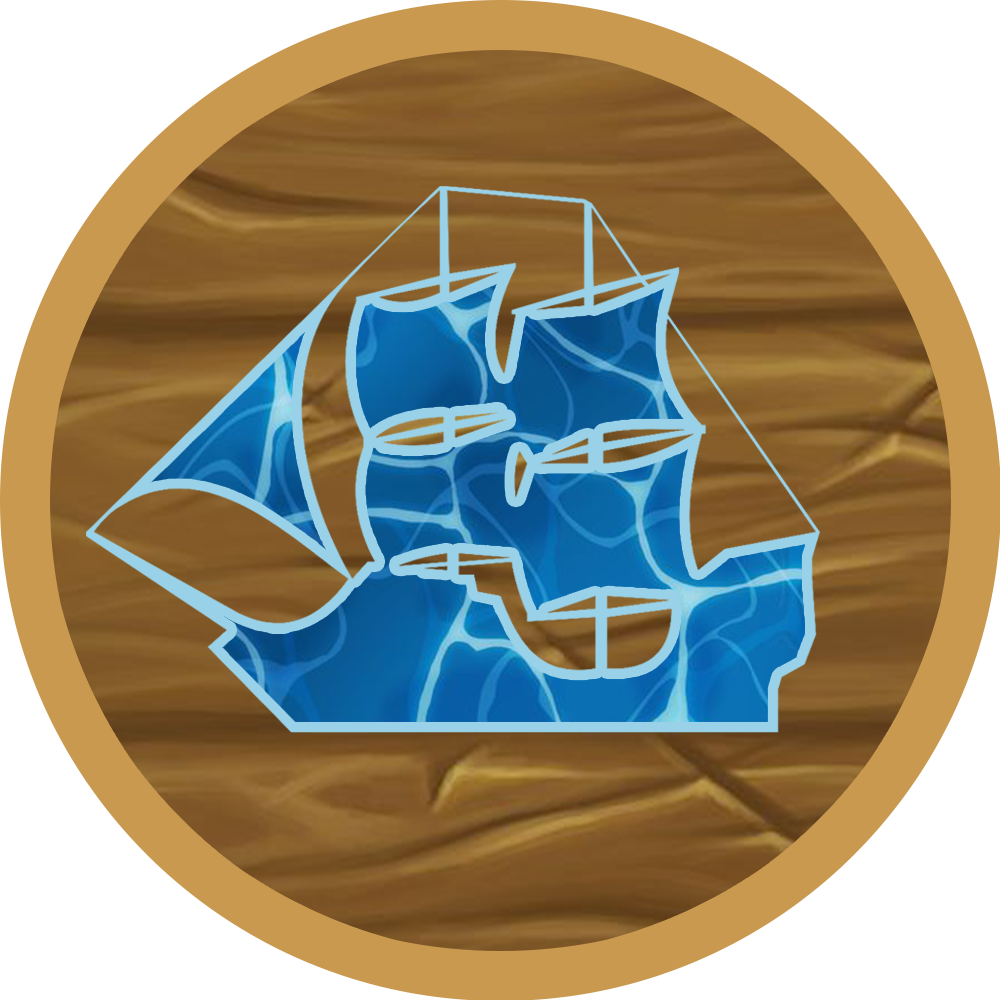
\includegraphics[width=2in]{Illustration/MenuUI/BoatButton.png}
    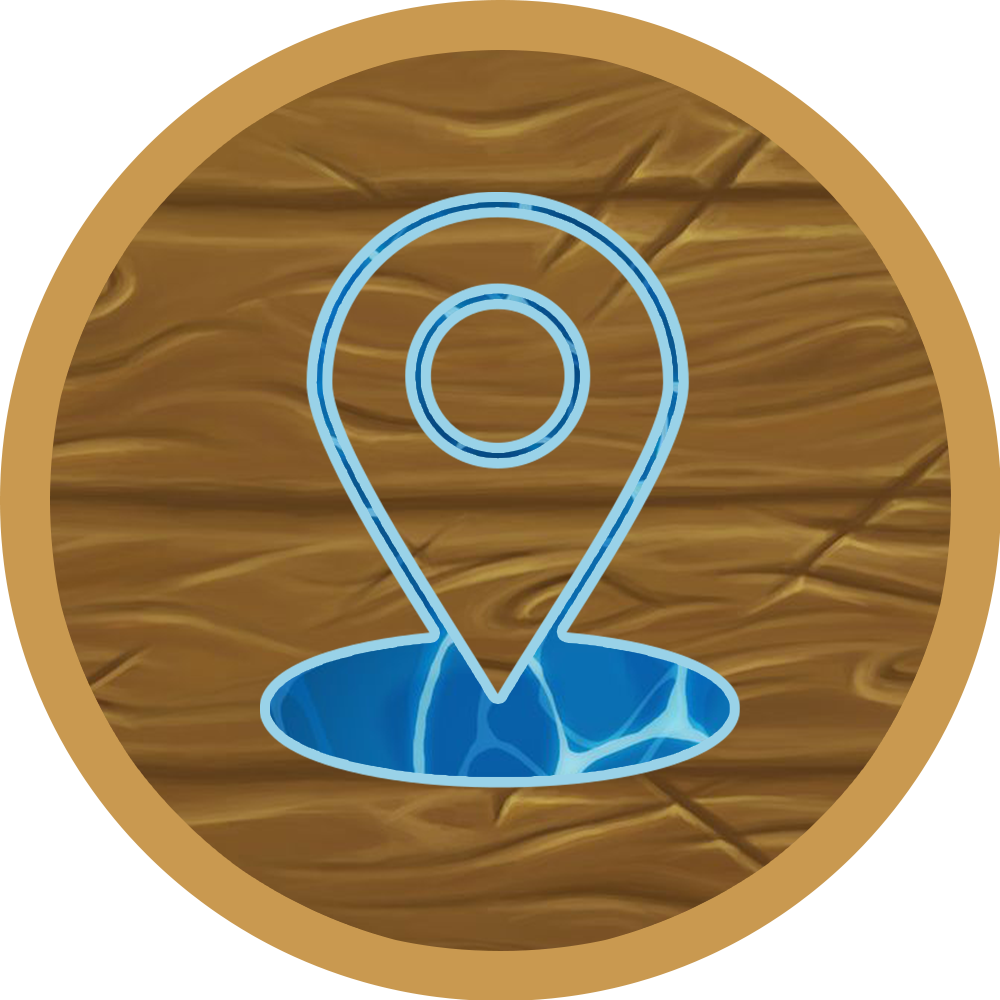
\includegraphics[width=2in]{Illustration/MenuUI/MapButton.png}
\end{center}

\subsection*{Water Simulation}
\begin{center}
    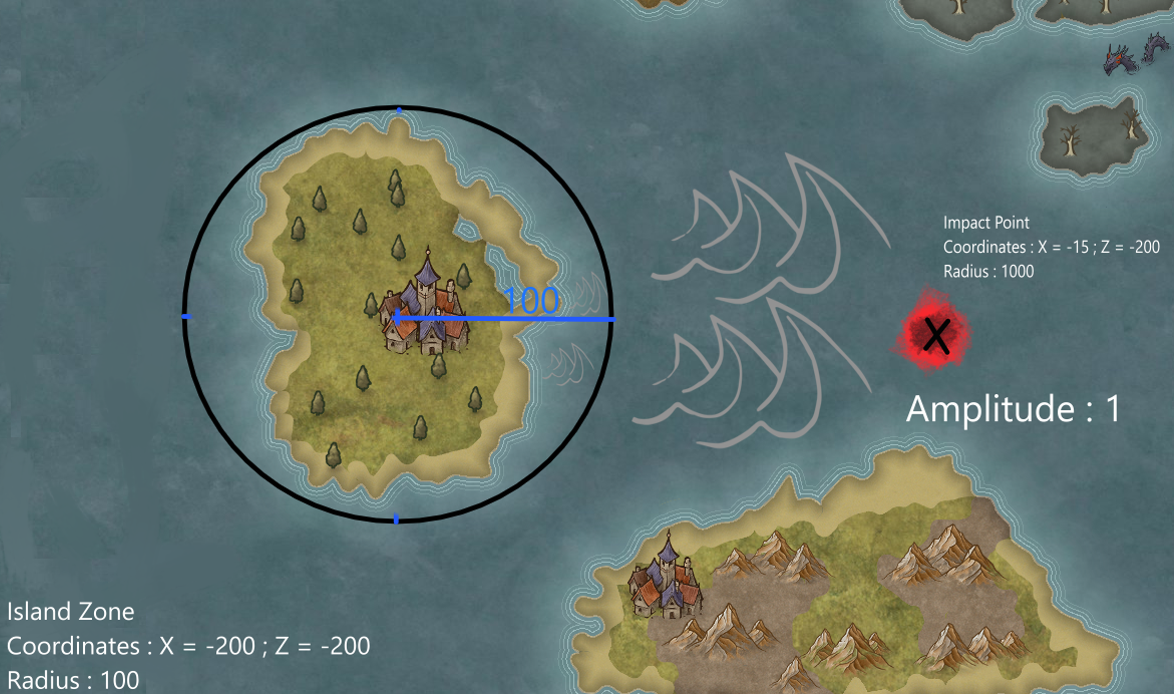
\includegraphics[width=5in]{Illustration/WaterSim/System_Eau.png}
    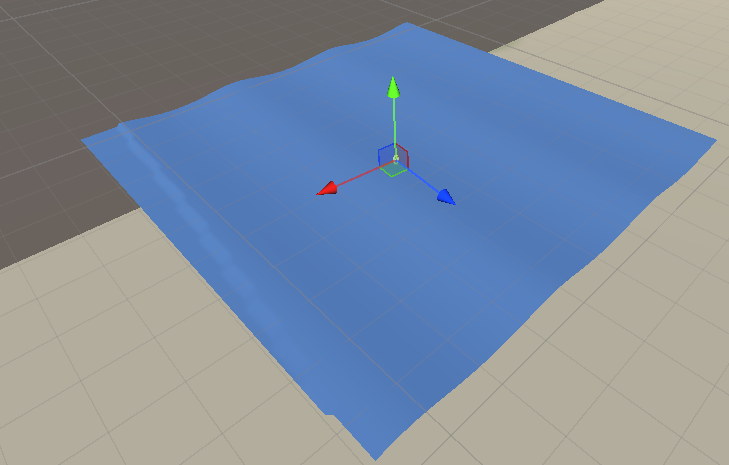
\includegraphics[width=5in]{Illustration/WaterSim/WaterSimulation.png}
\end{center}

\subsection*{Boat Simulation}
\begin{center}
    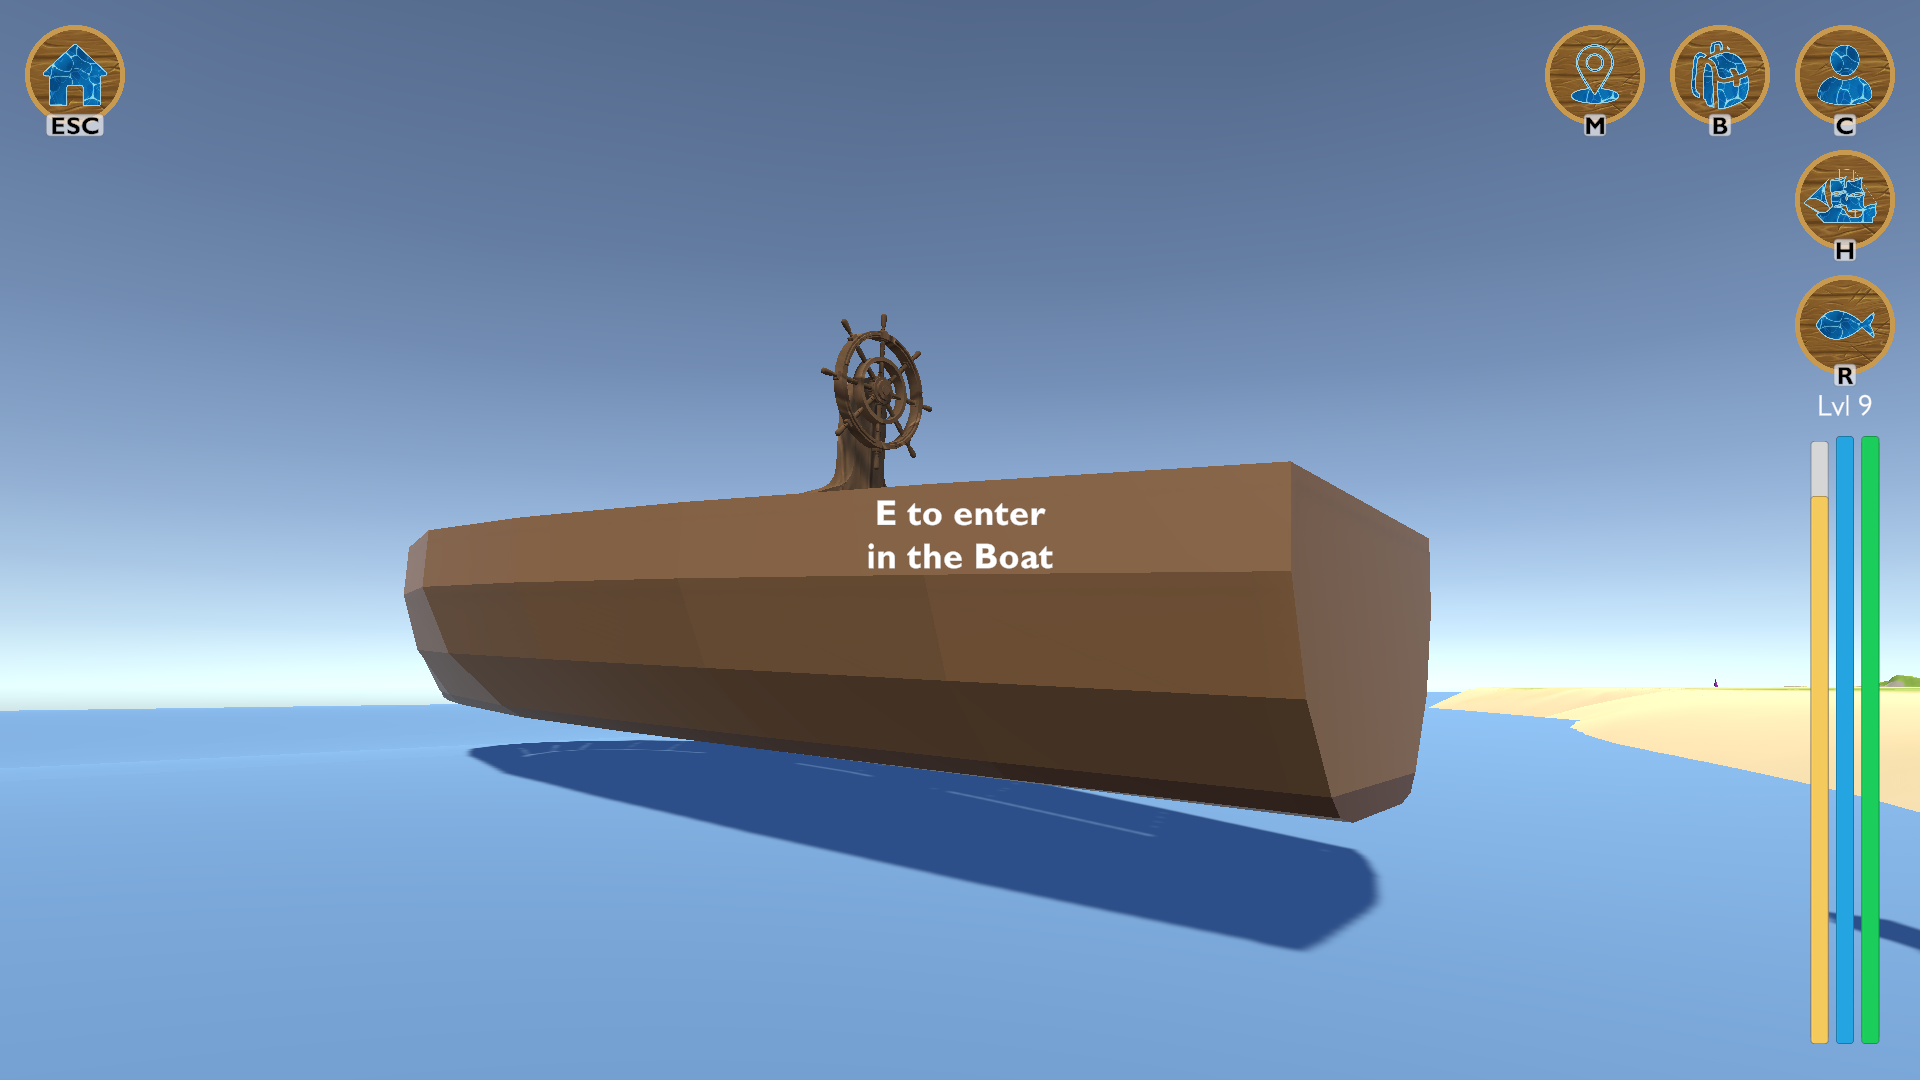
\includegraphics[width=5in]{Illustration/BoatMovement/EnterBoat.png}
    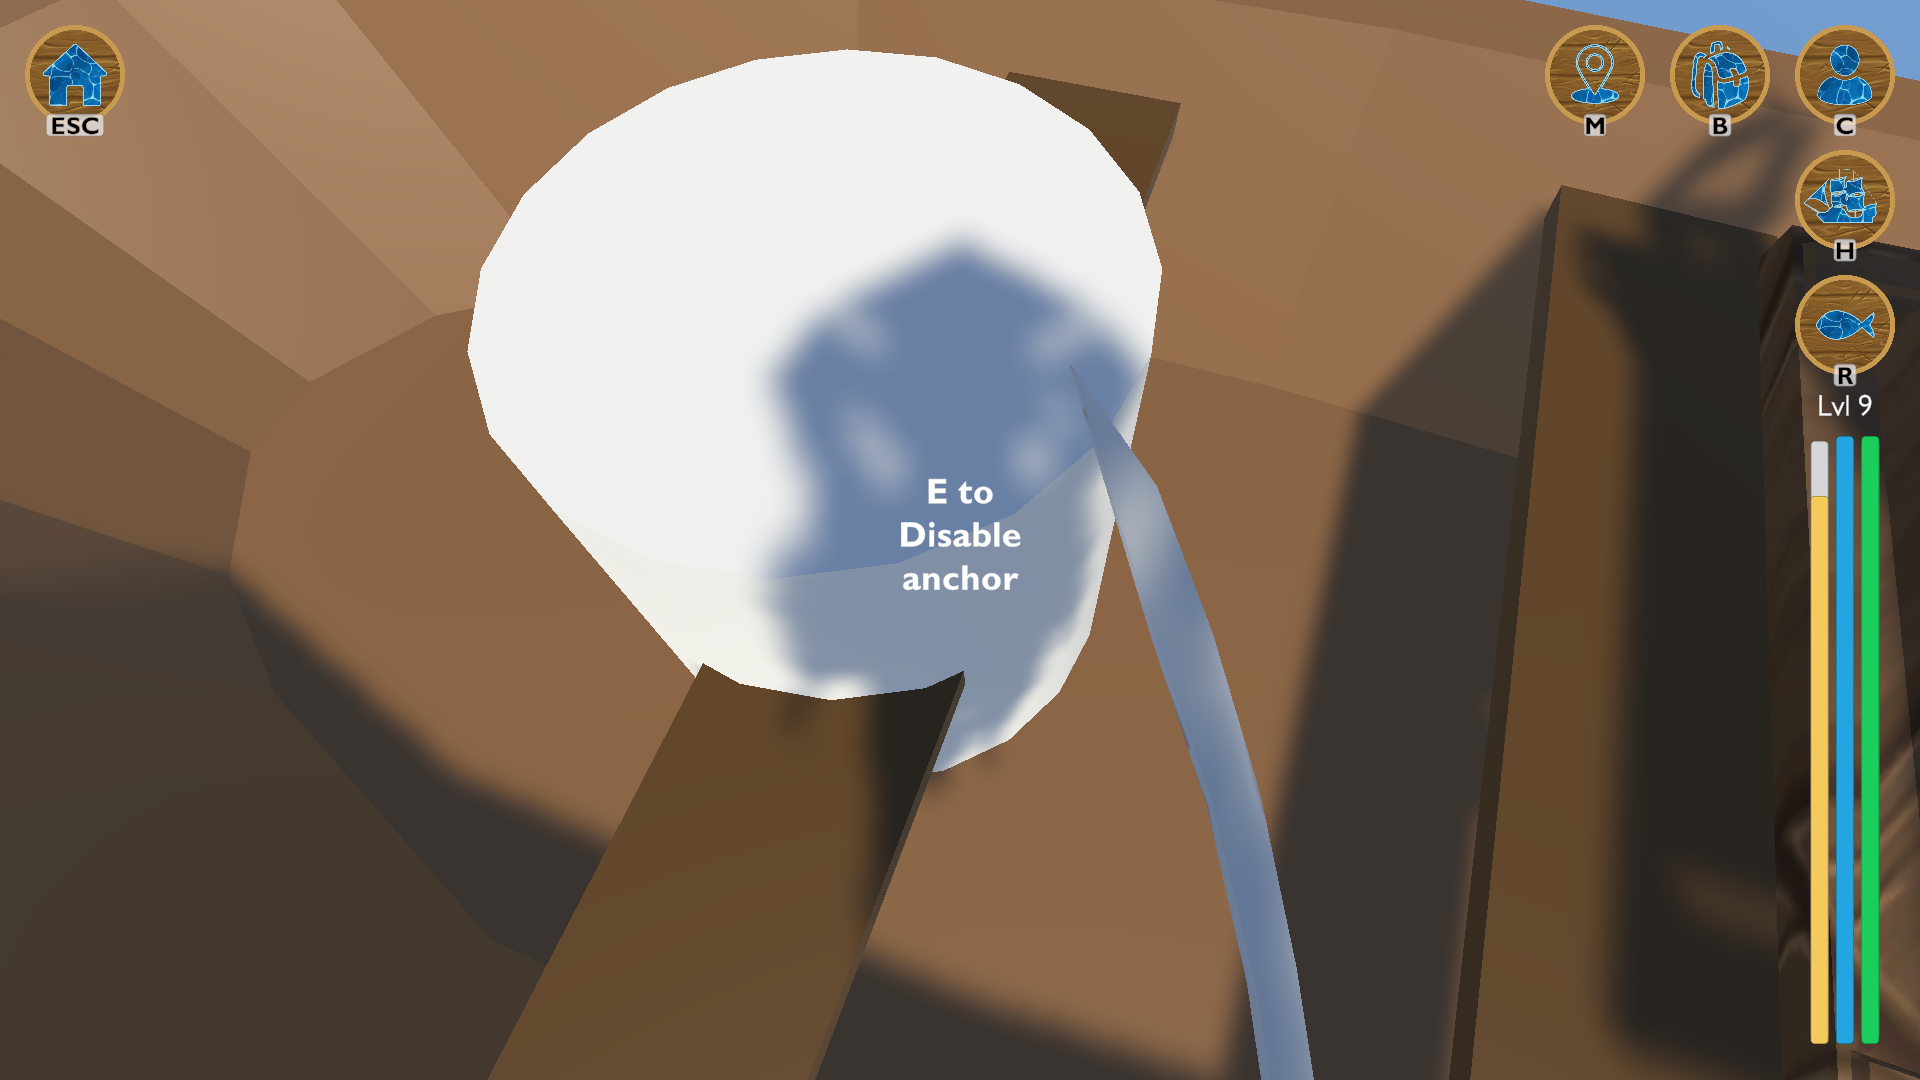
\includegraphics[width=5in]{Illustration/BoatMovement/Anchor.png}
    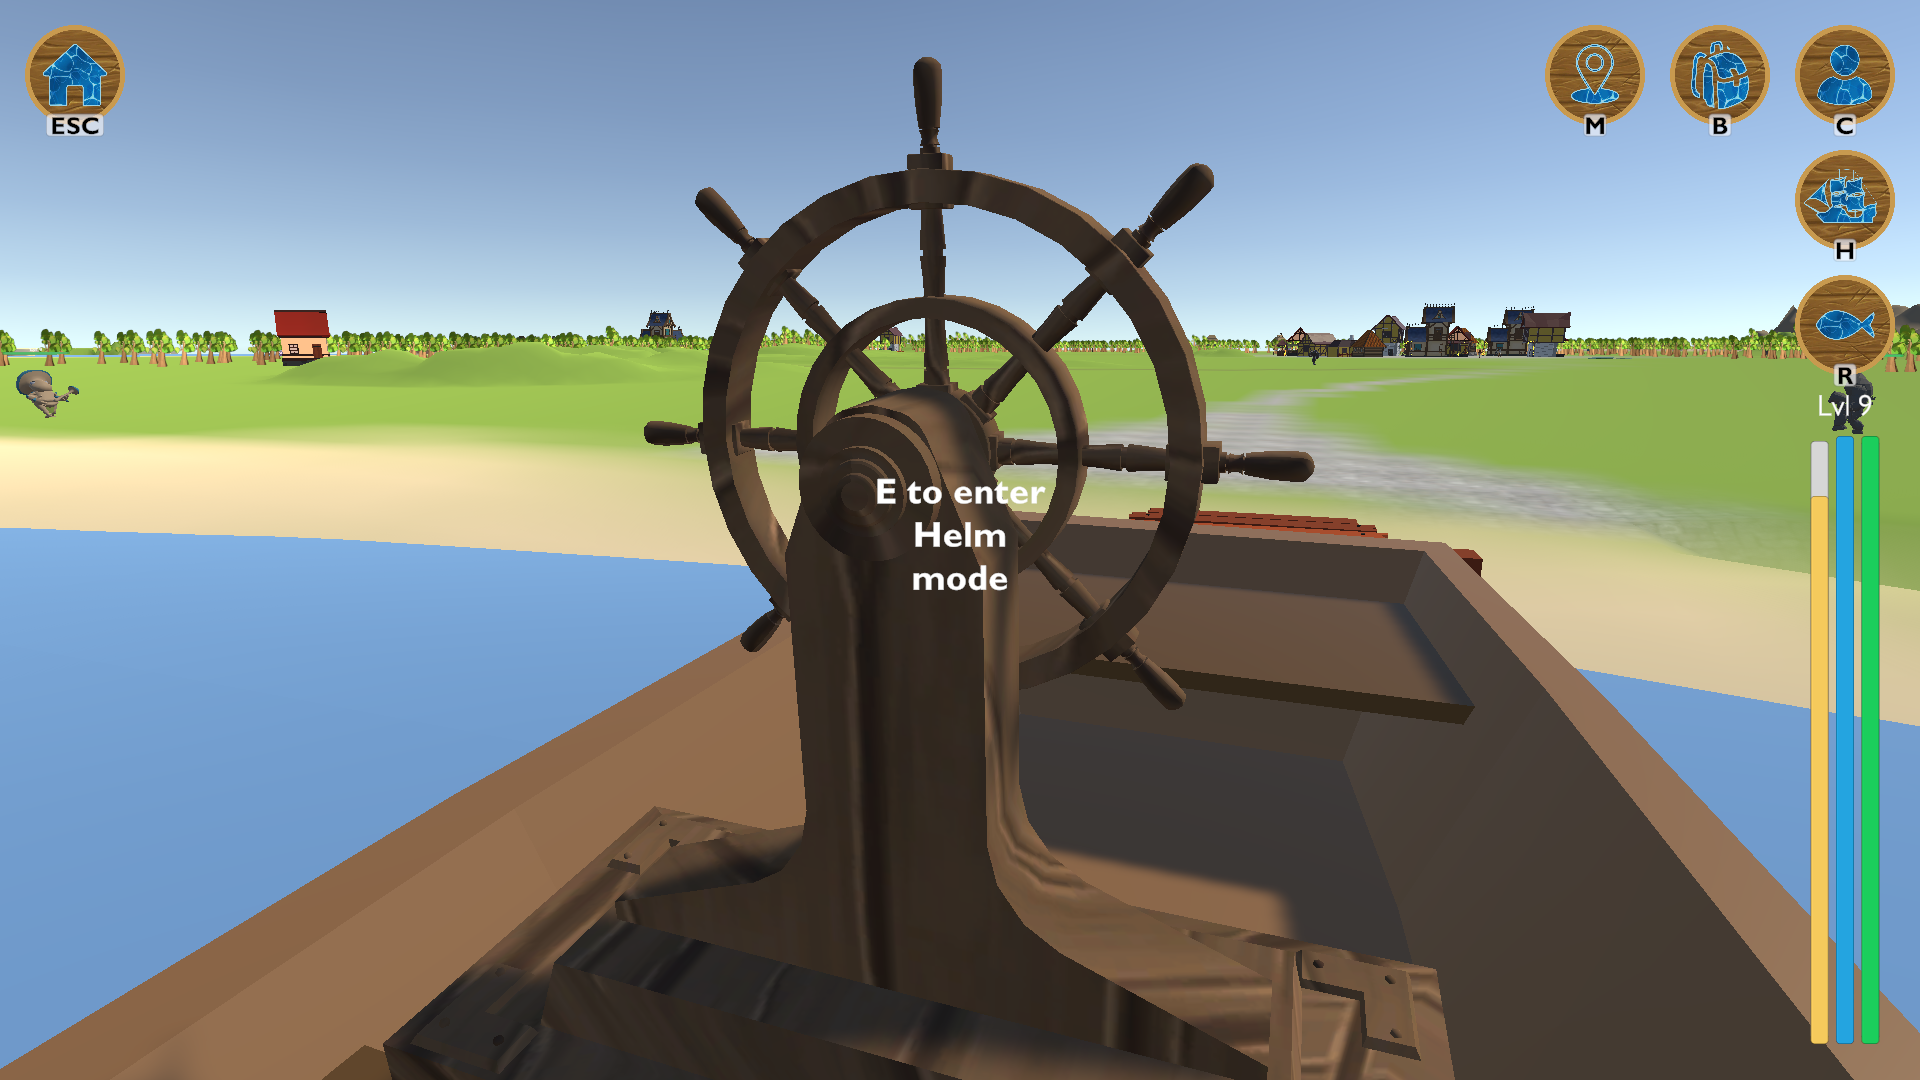
\includegraphics[width=5in]{Illustration/BoatMovement/Helm.png}
\end{center}

\subsection*{AI}
\begin{center}
    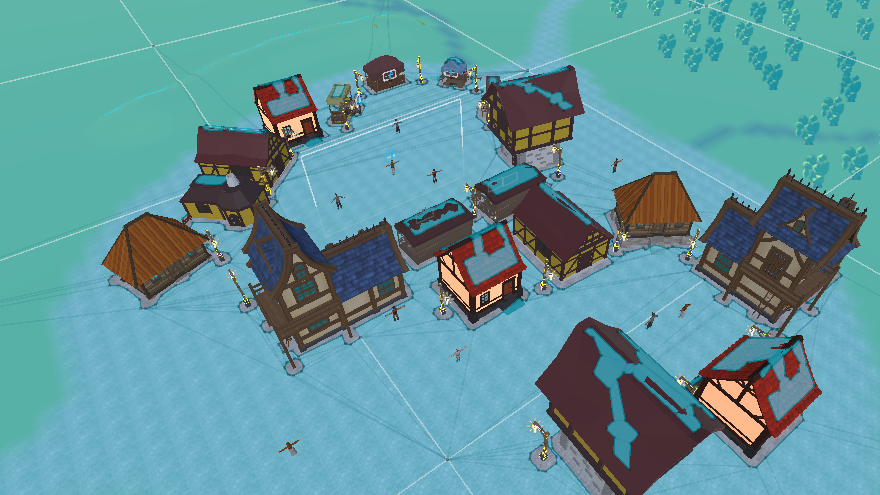
\includegraphics[width=5in]{Illustration/AI/NavMesh1.png}    
    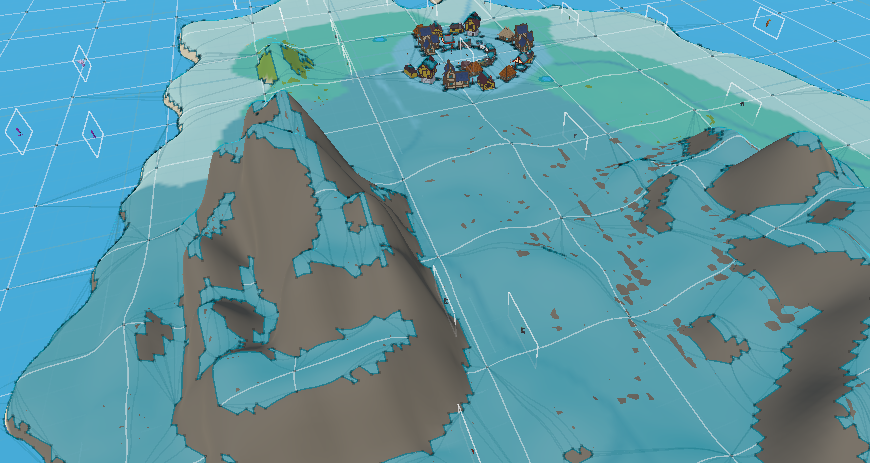
\includegraphics[width=5in]{Illustration/AI/NavMesh2.png}    
    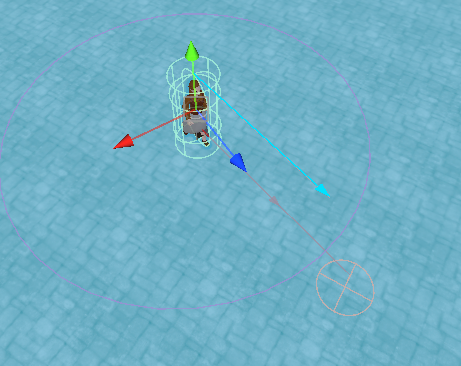
\includegraphics[width=5in]{Illustration/AI/Passiv.png}    
    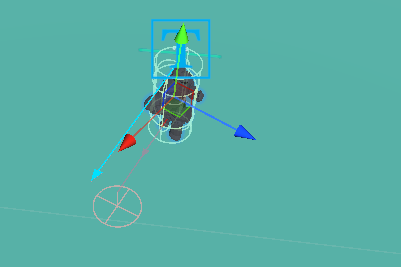
\includegraphics[width=5in]{Illustration/AI/Offensiv.png}    
\end{center}

\subsection*{Combat System}
\begin{center}
    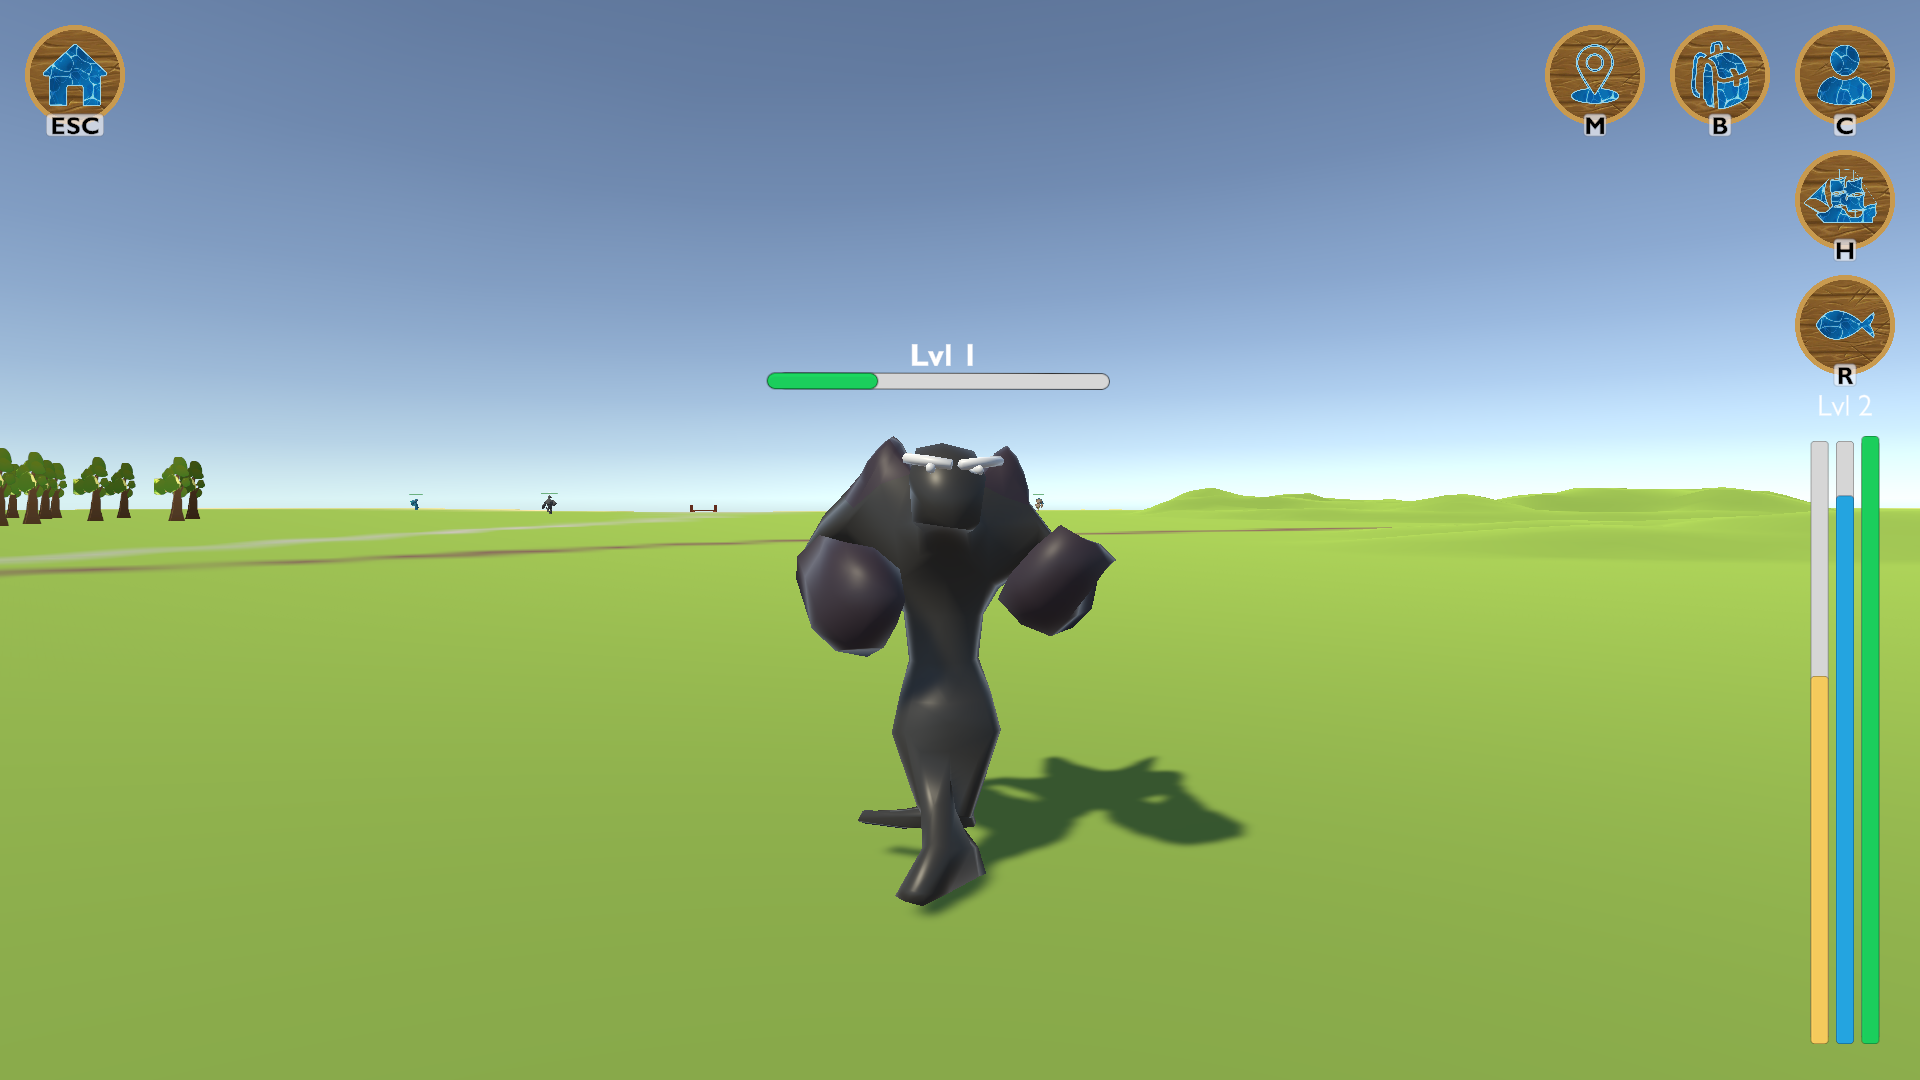
\includegraphics[width=5in]{Illustration/Combat/TerestrialEnemy.png}
    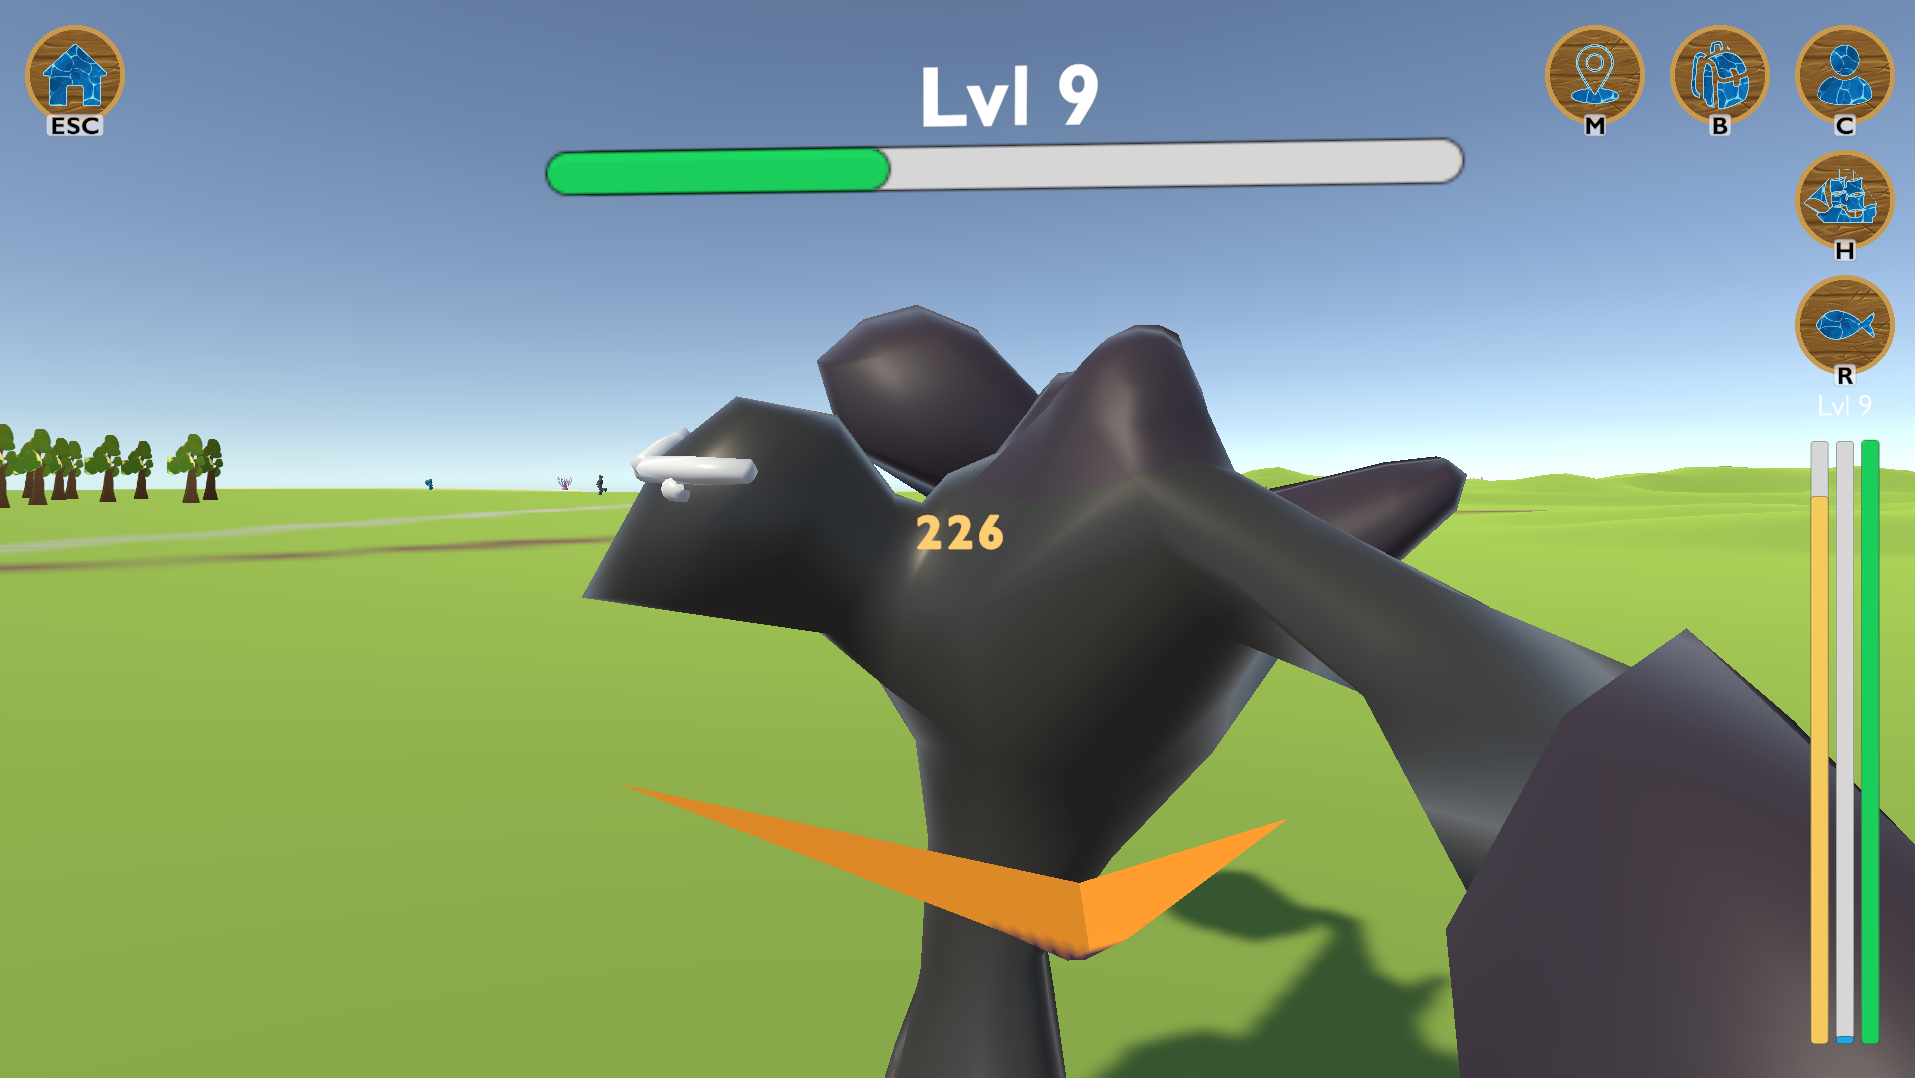
\includegraphics[width=5in]{Illustration/Combat/CombatTerestrial.png}
    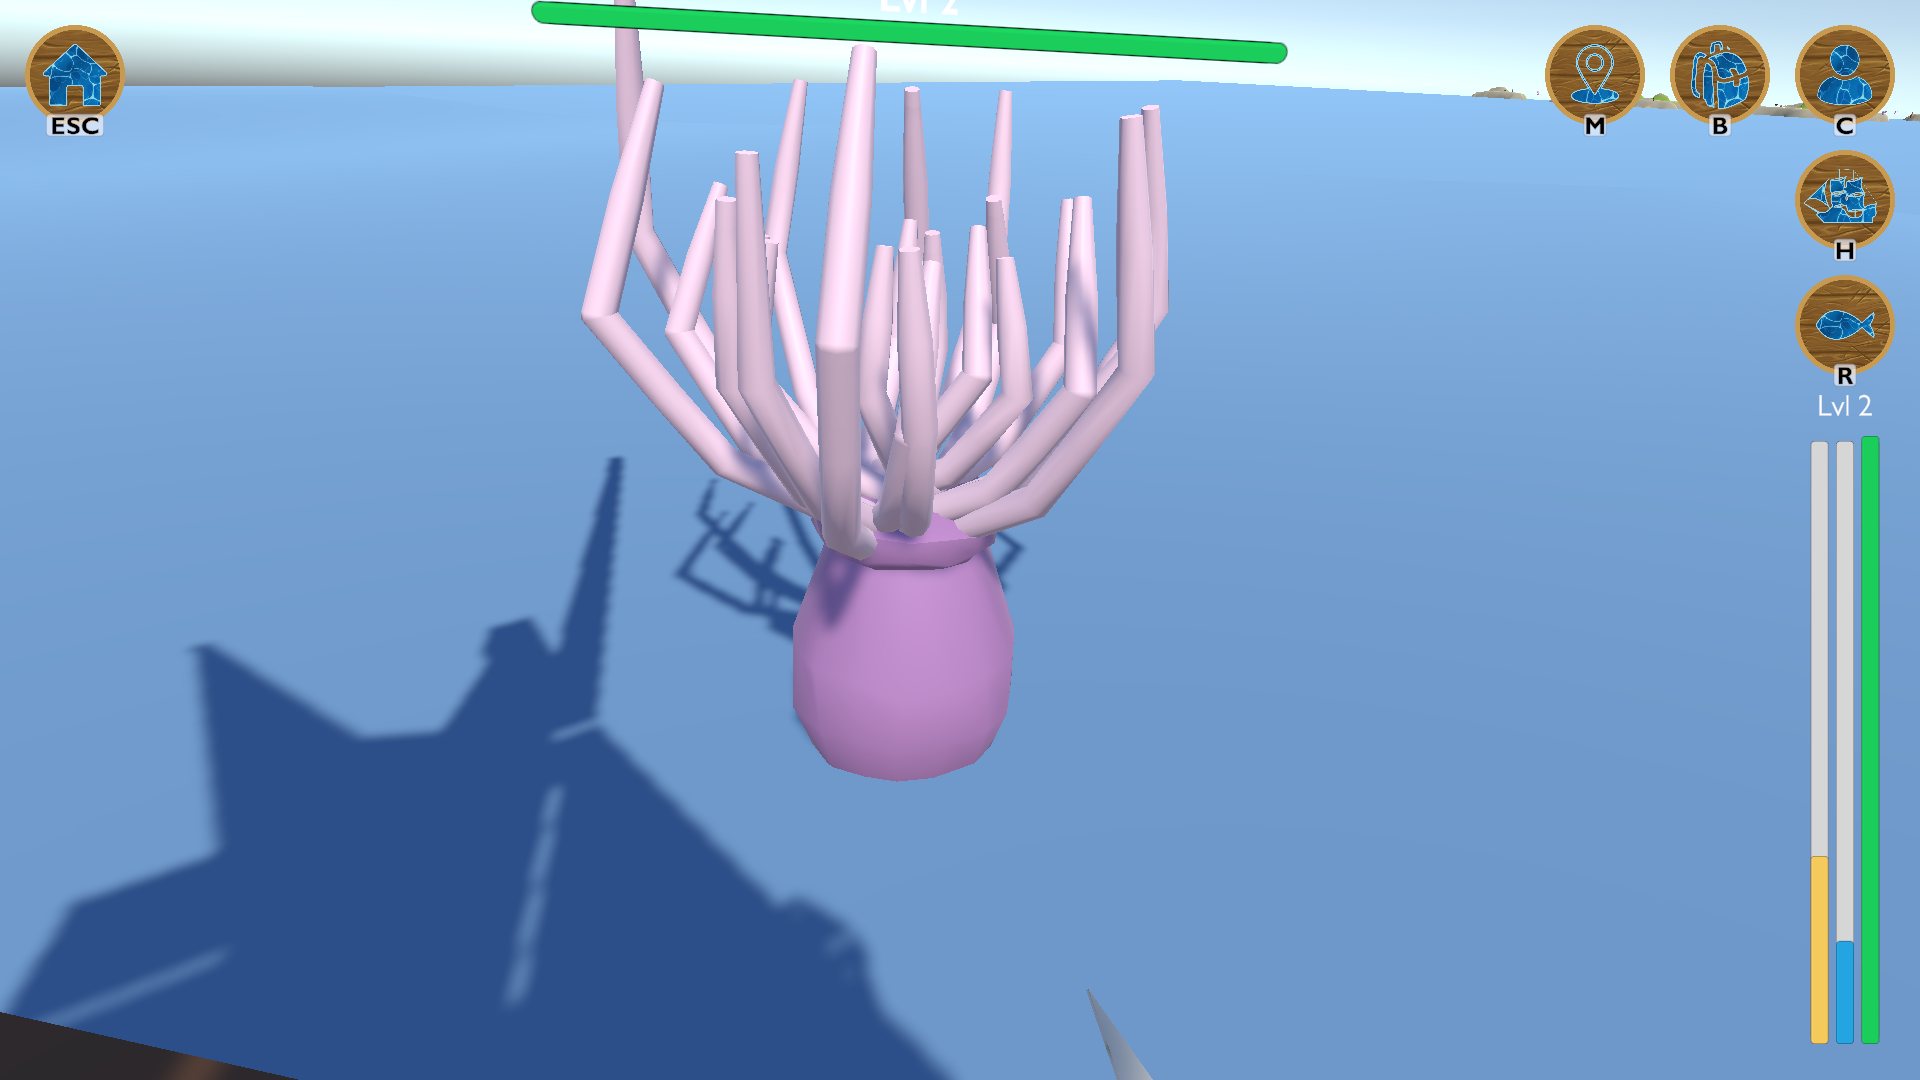
\includegraphics[width=5in]{Illustration/Combat/MaritimeEnemy.png}
    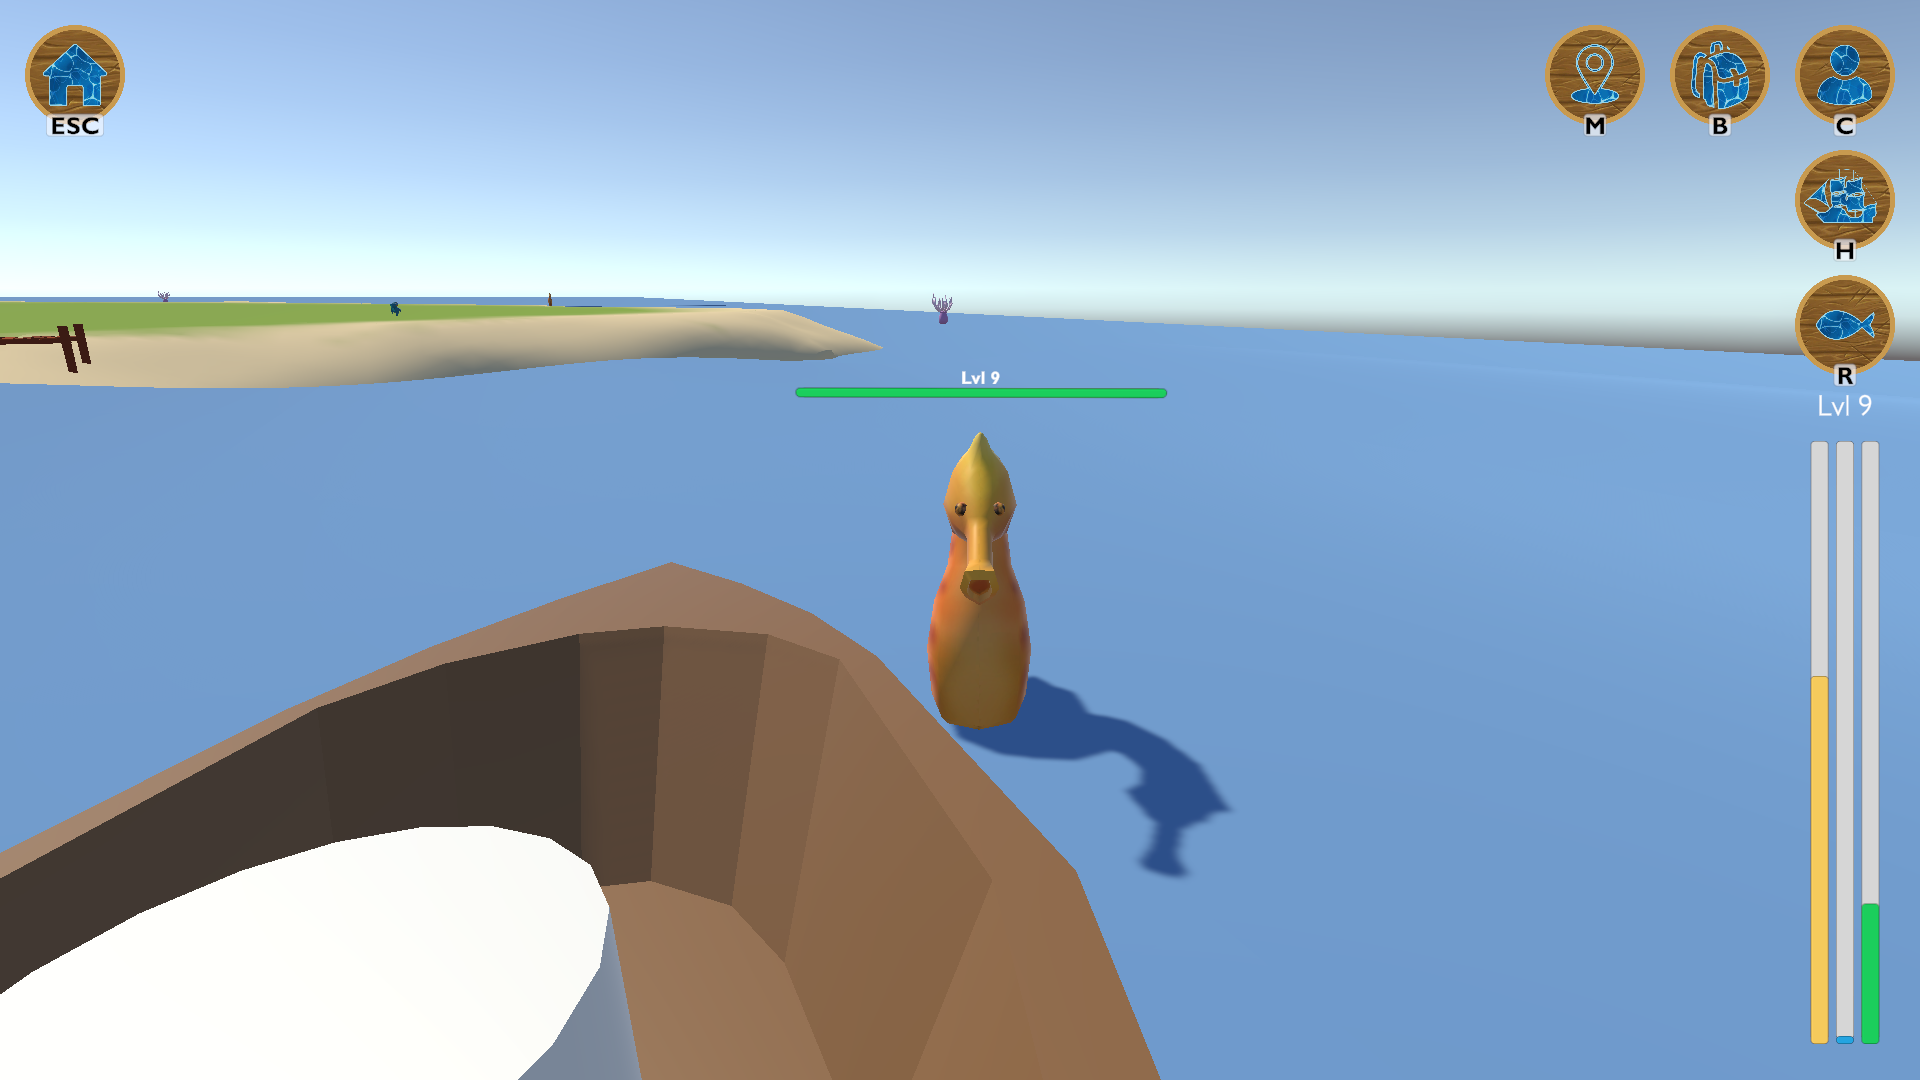
\includegraphics[width=5in]{Illustration/Combat/CombatMaritim.png}
\end{center}

\subsection*{Map}
\begin{center}
    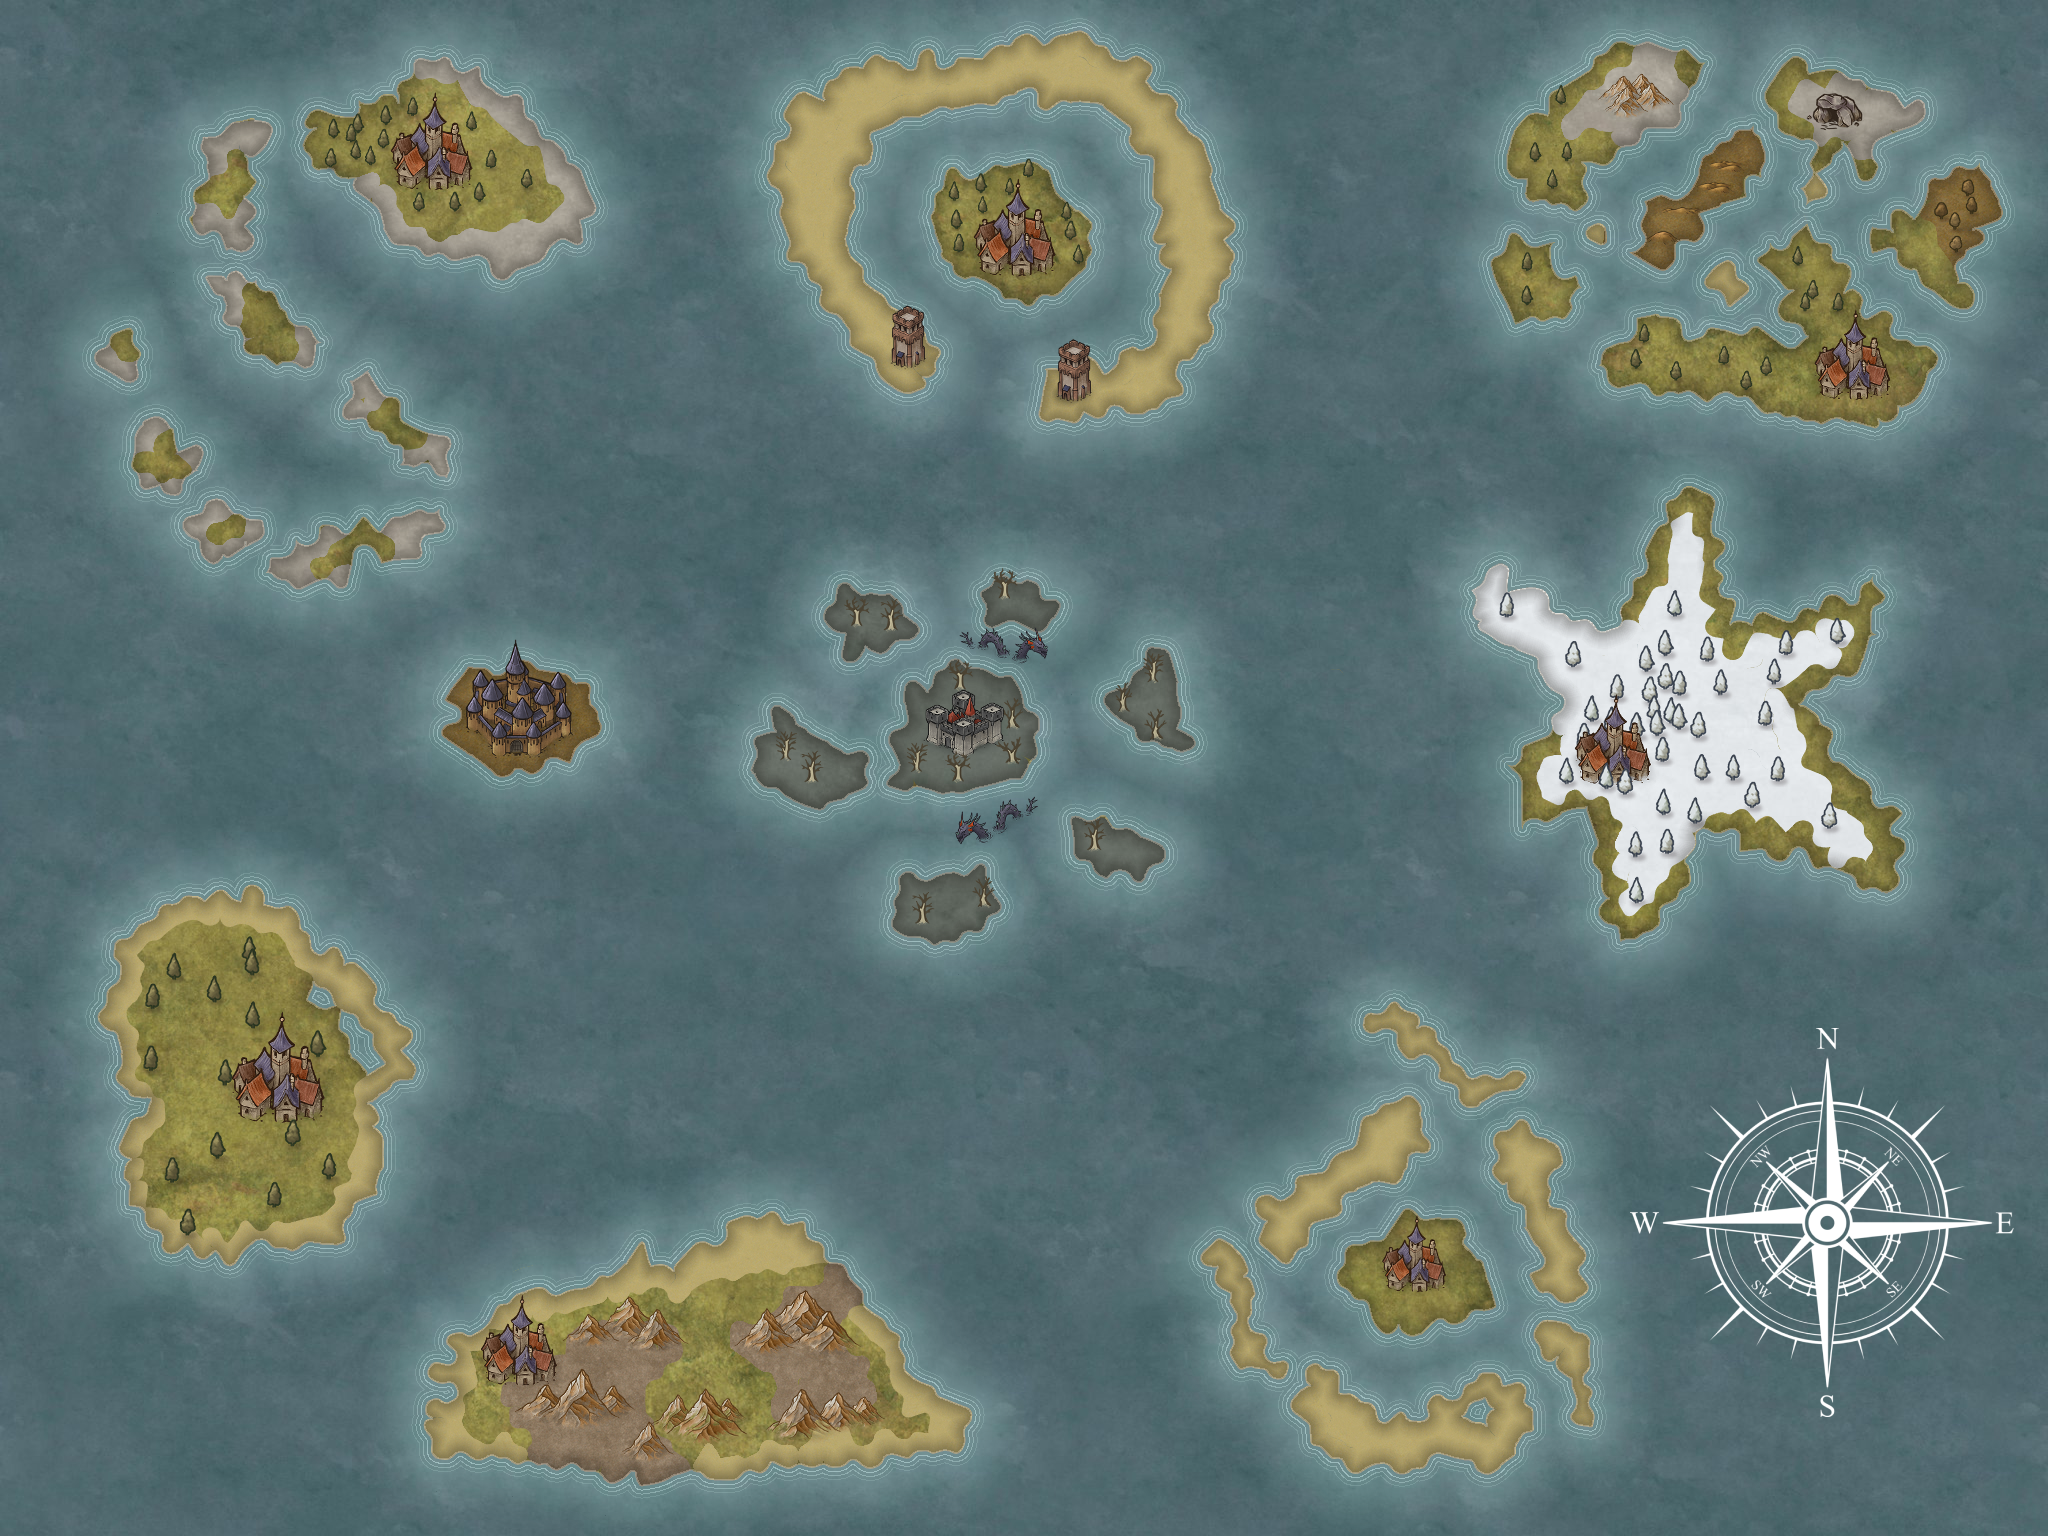
\includegraphics[width=5in]{Illustration/Map/2dMap.png}
    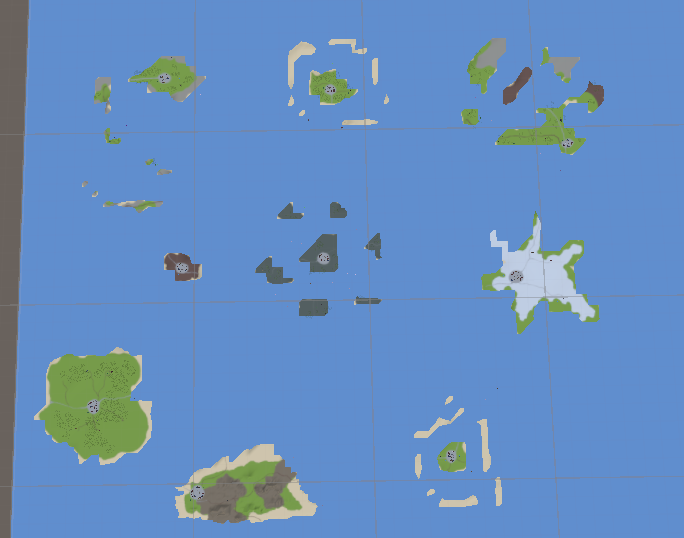
\includegraphics[width=5in]{Illustration/Map/Full.png}
    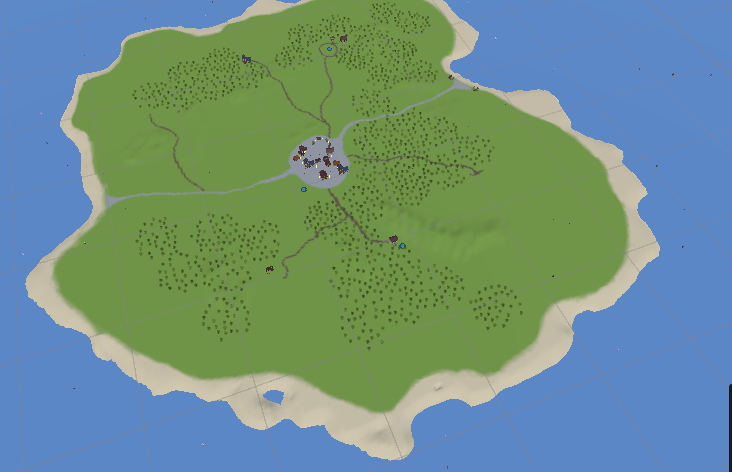
\includegraphics[width=5in]{Illustration/Map/Island.png}
    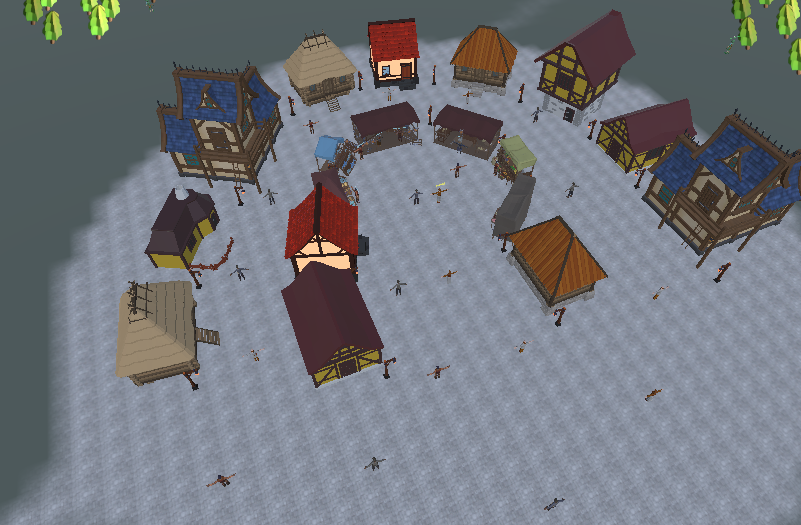
\includegraphics[width=5in]{Illustration/Map/Village.png}
    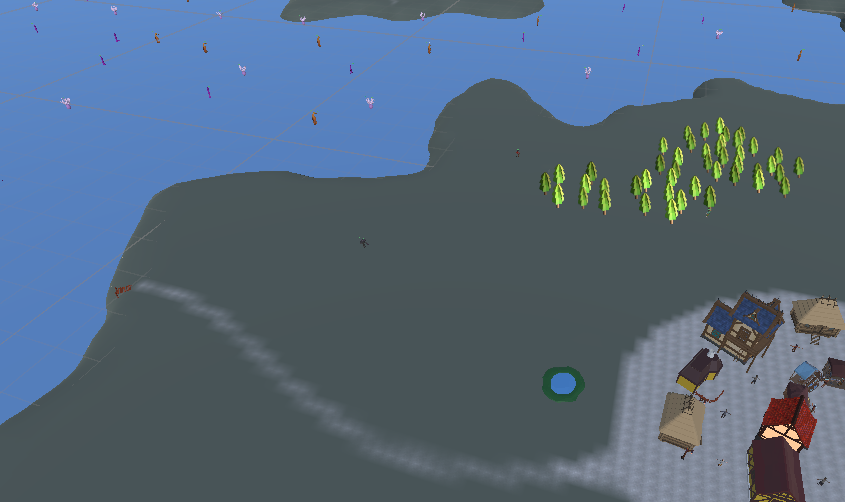
\includegraphics[width=5in]{Illustration/Map/Other.png}
    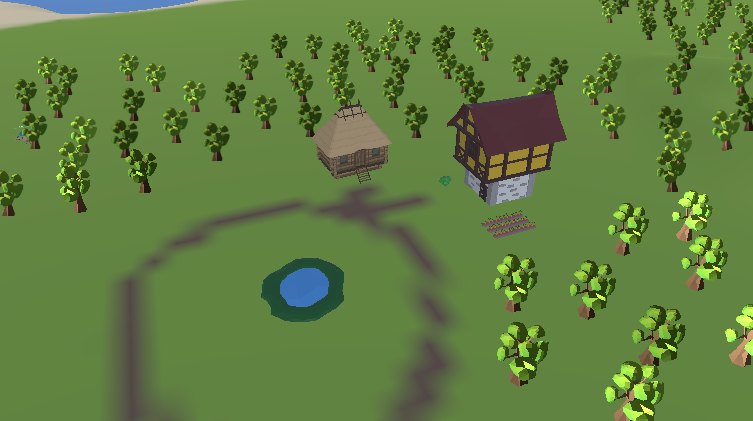
\includegraphics[width=5in]{Illustration/Map/other2.png}
\end{center}

\subsection*{Localisation system}
\begin{center}
    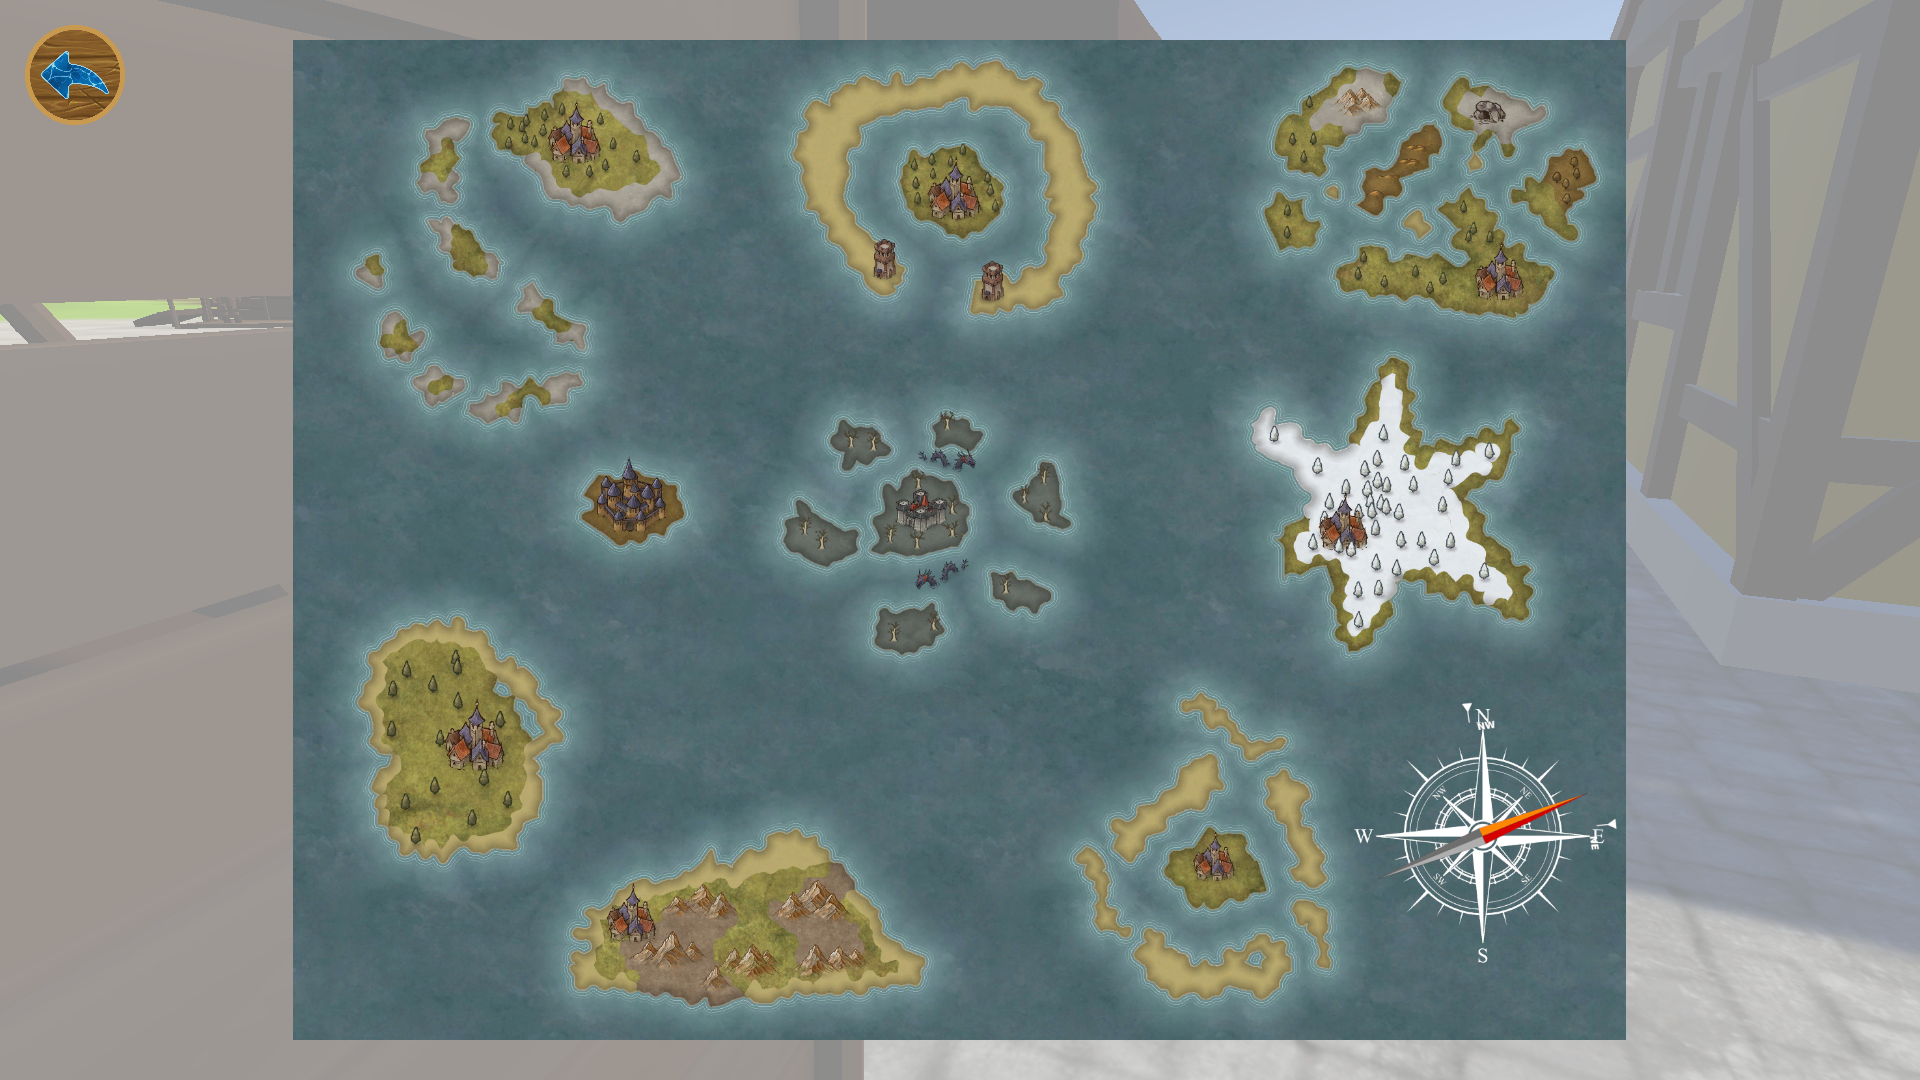
\includegraphics[width=5in]{Illustration/Localization/Loc.png}
\end{center}

\subsection*{Shops}
\begin{center}
    
\includegraphics[width=5in]{Illustration/Shops/Shop1.png}
    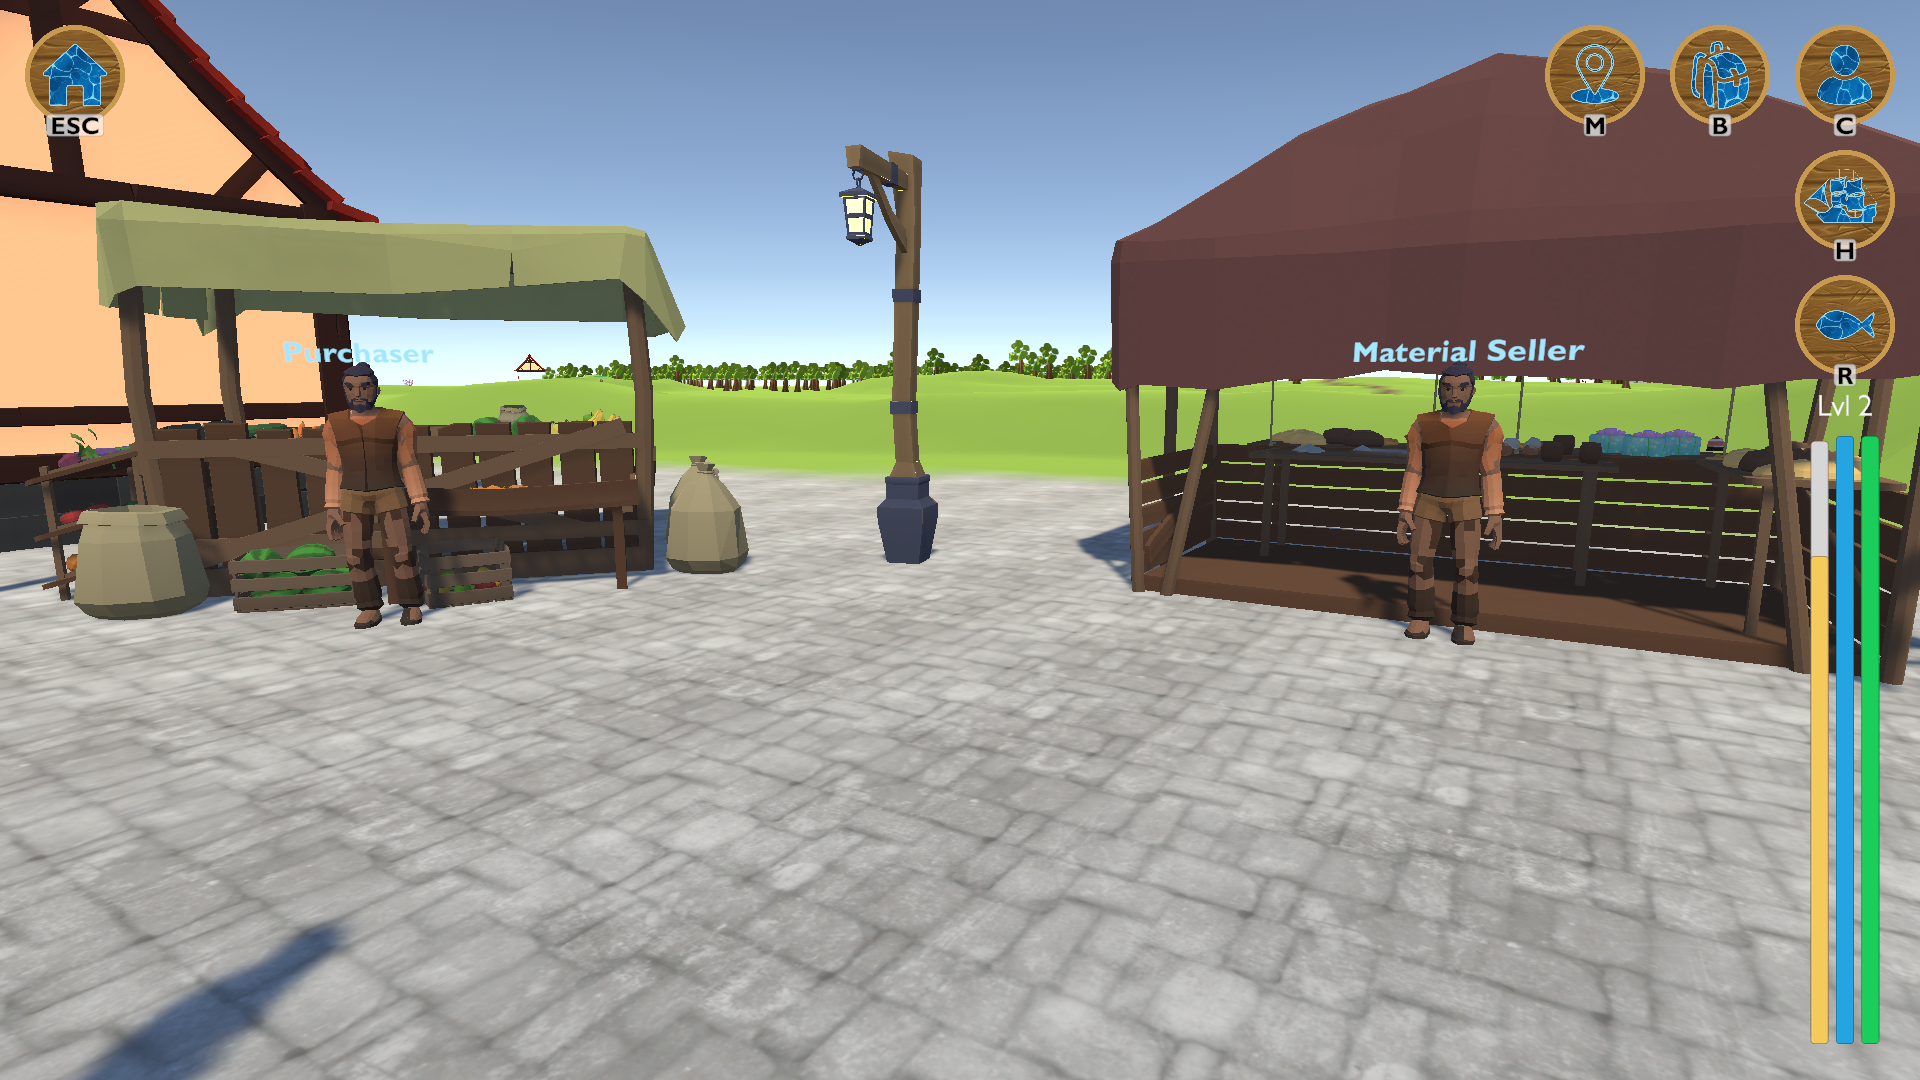
\includegraphics[width=5in]{Illustration/Shops/Shop2.png}
    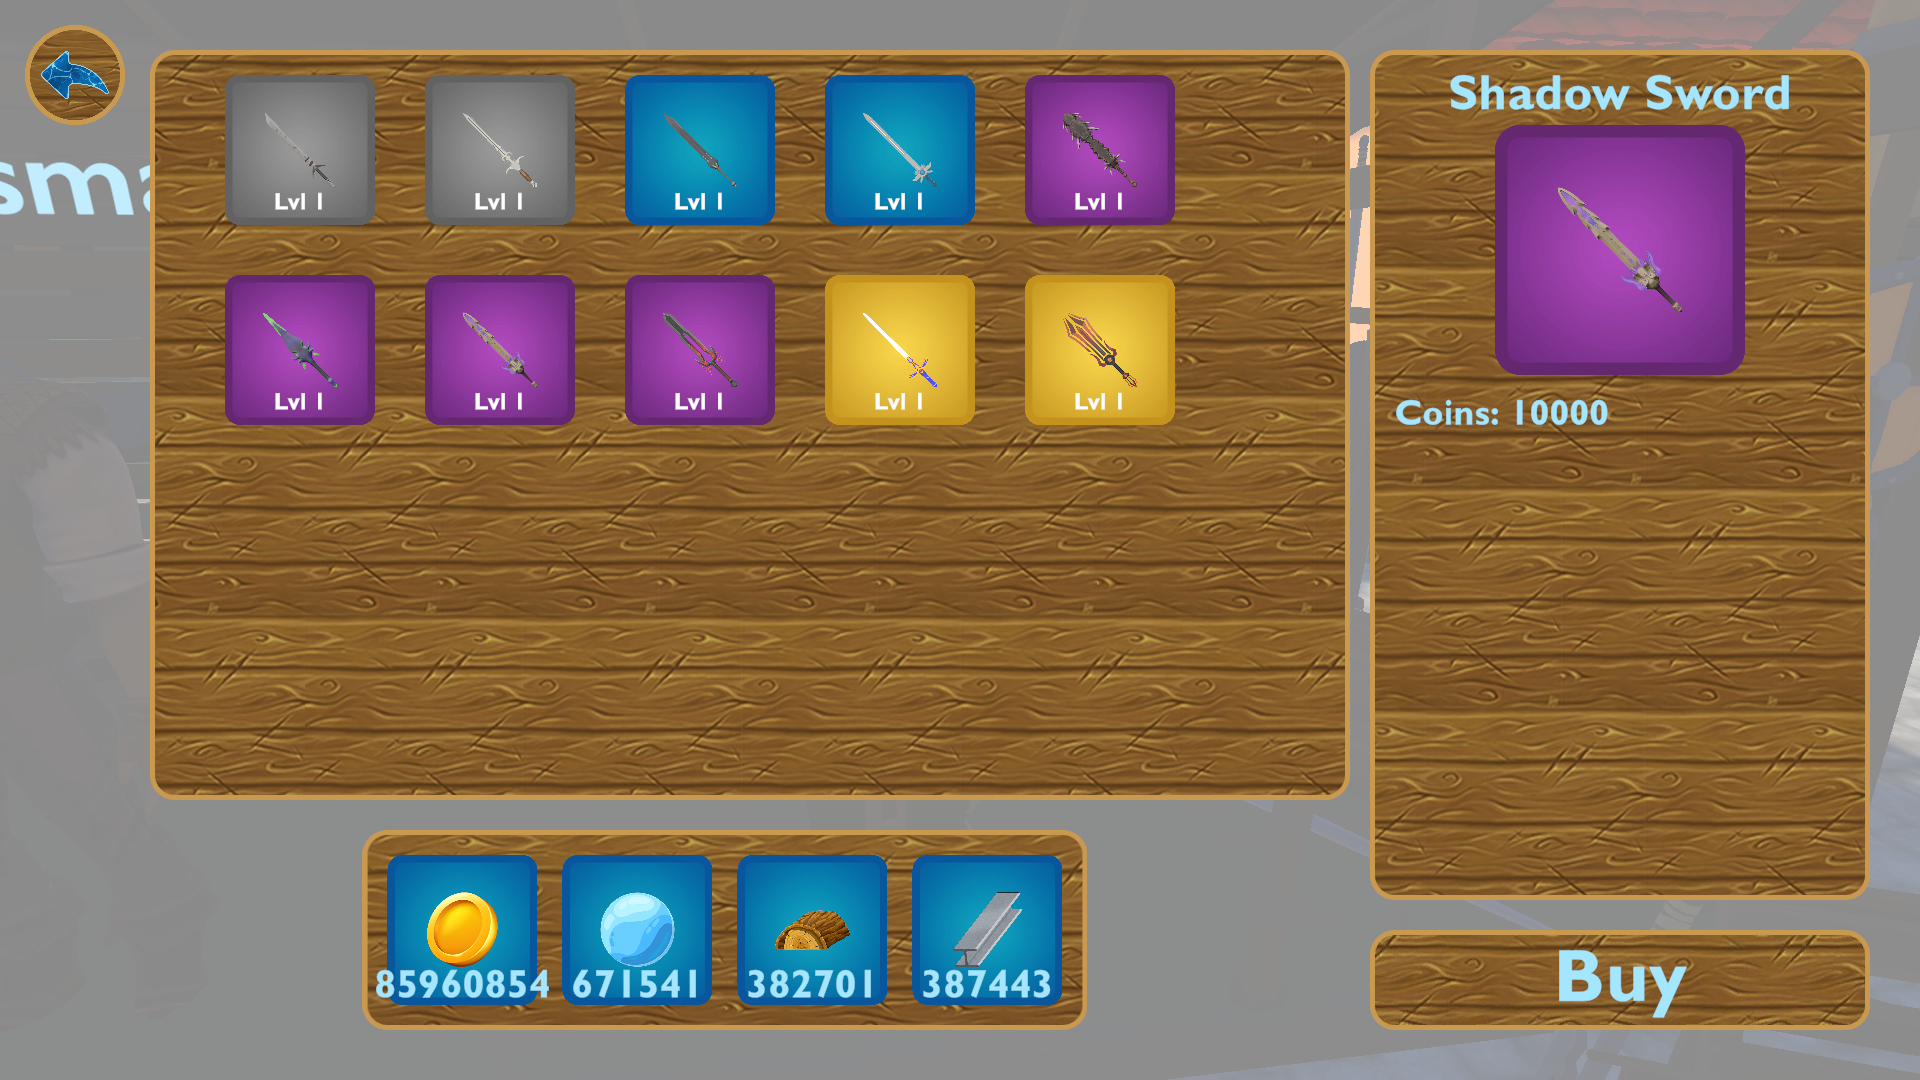
\includegraphics[width=5in]{Illustration/Shops/Armorer.png}
    
\includegraphics[width=5in]{Illustration/Shops/Mage.png}
    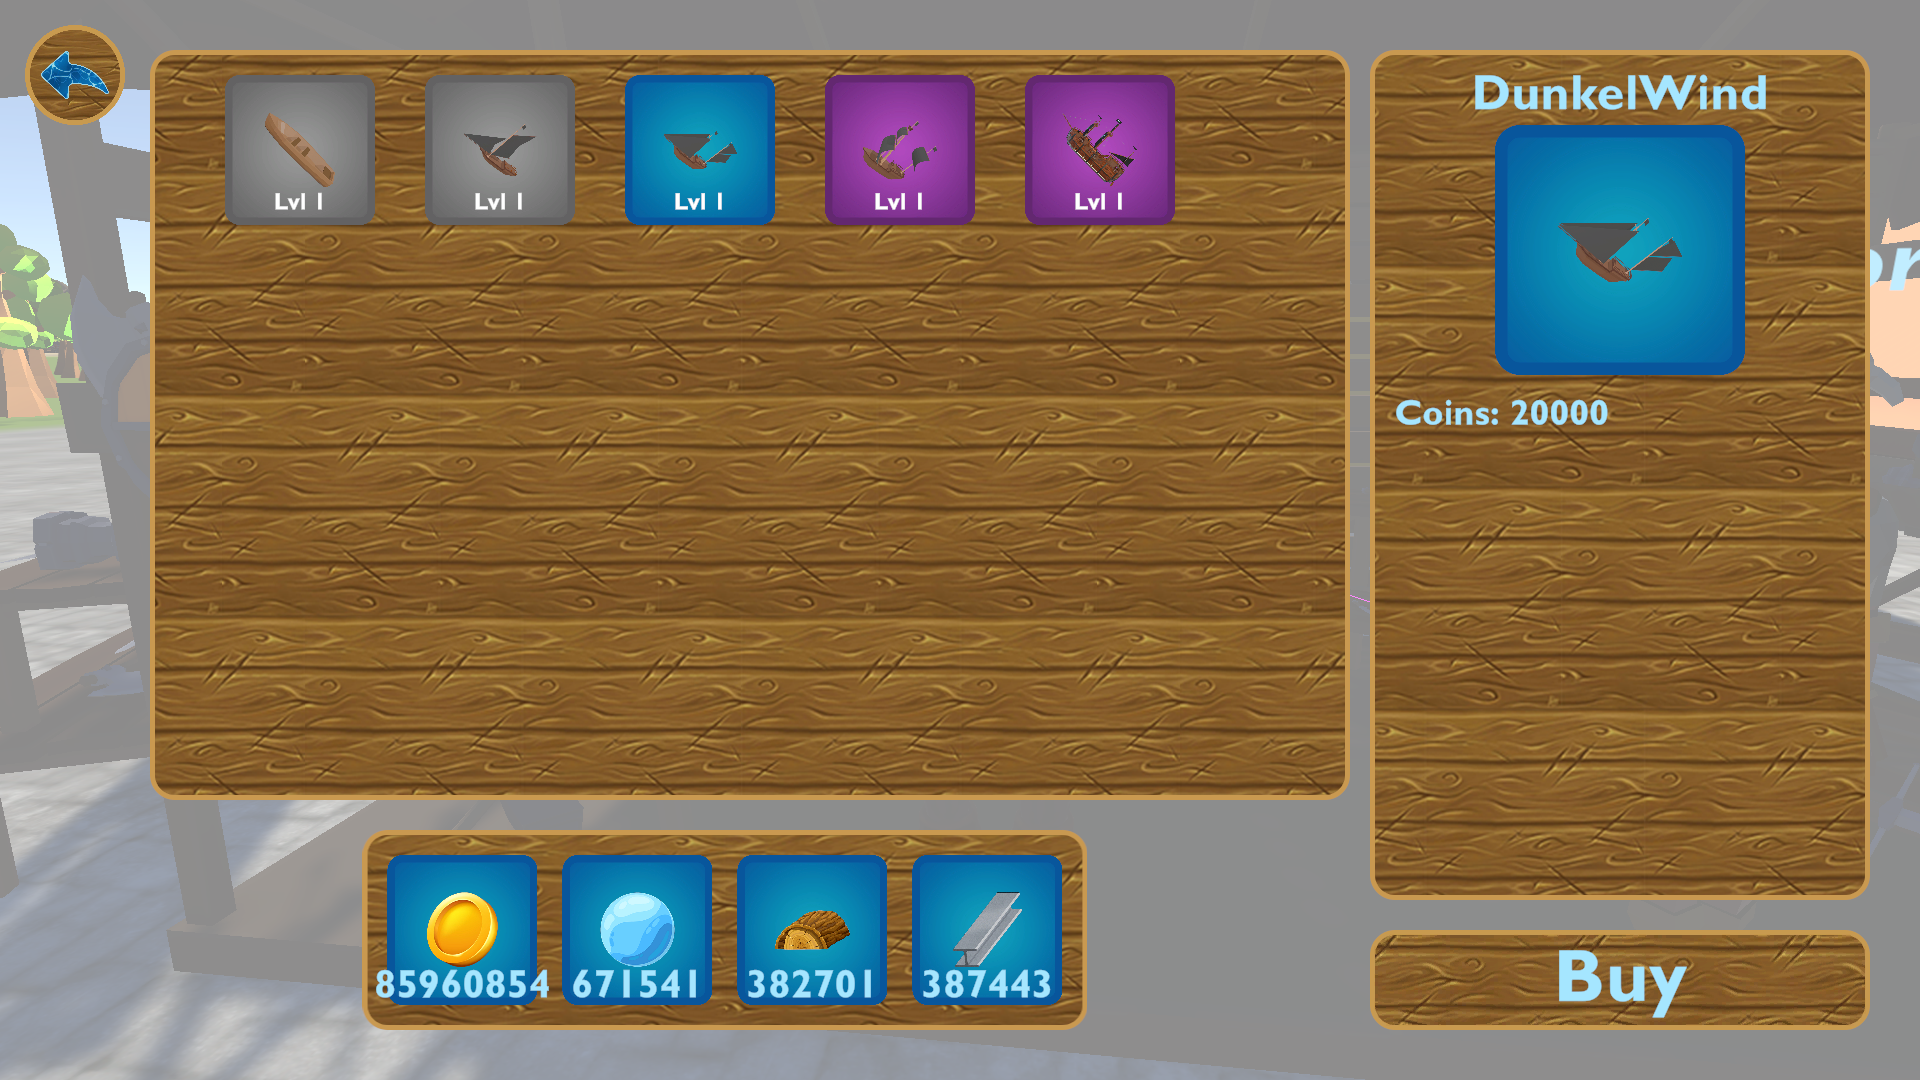
\includegraphics[width=5in]{Illustration/Shops/BoatSalesman.png}
    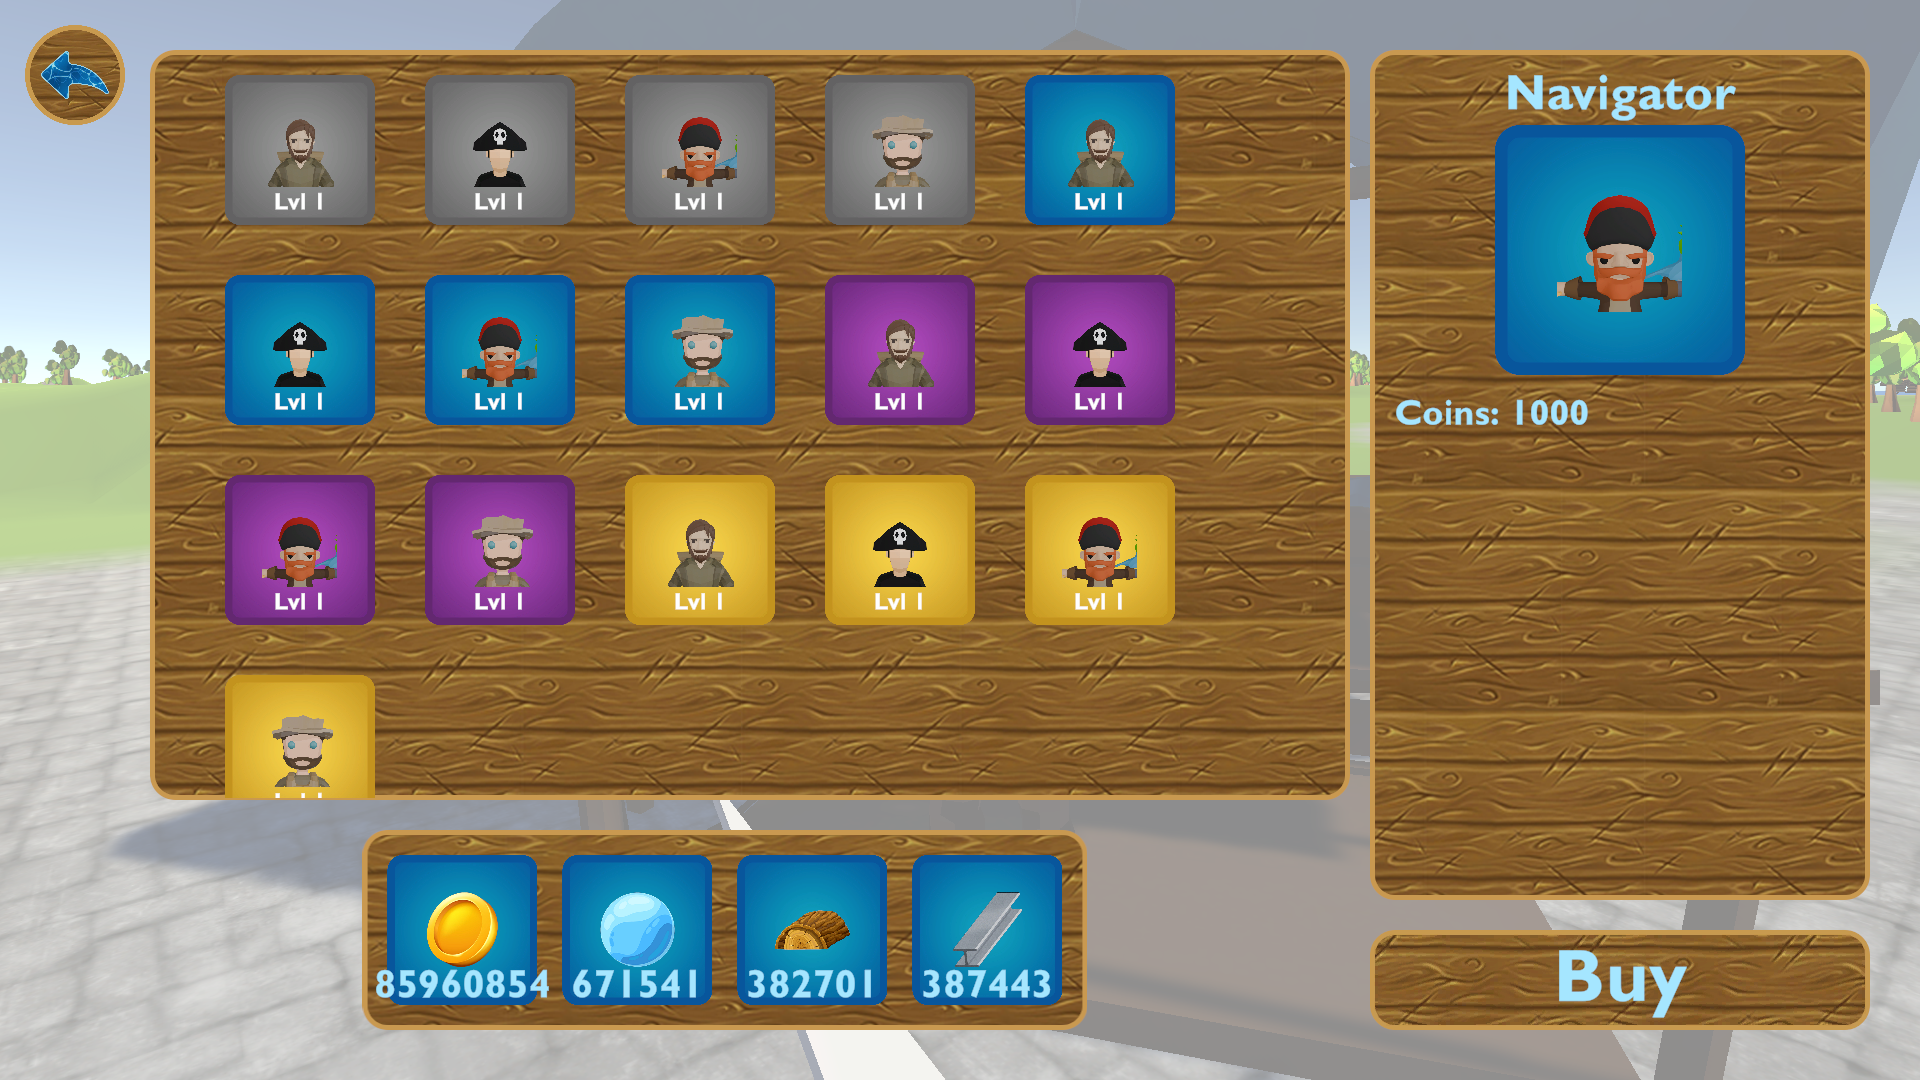
\includegraphics[width=5in]{Illustration/Shops/CrewAgent.png}
    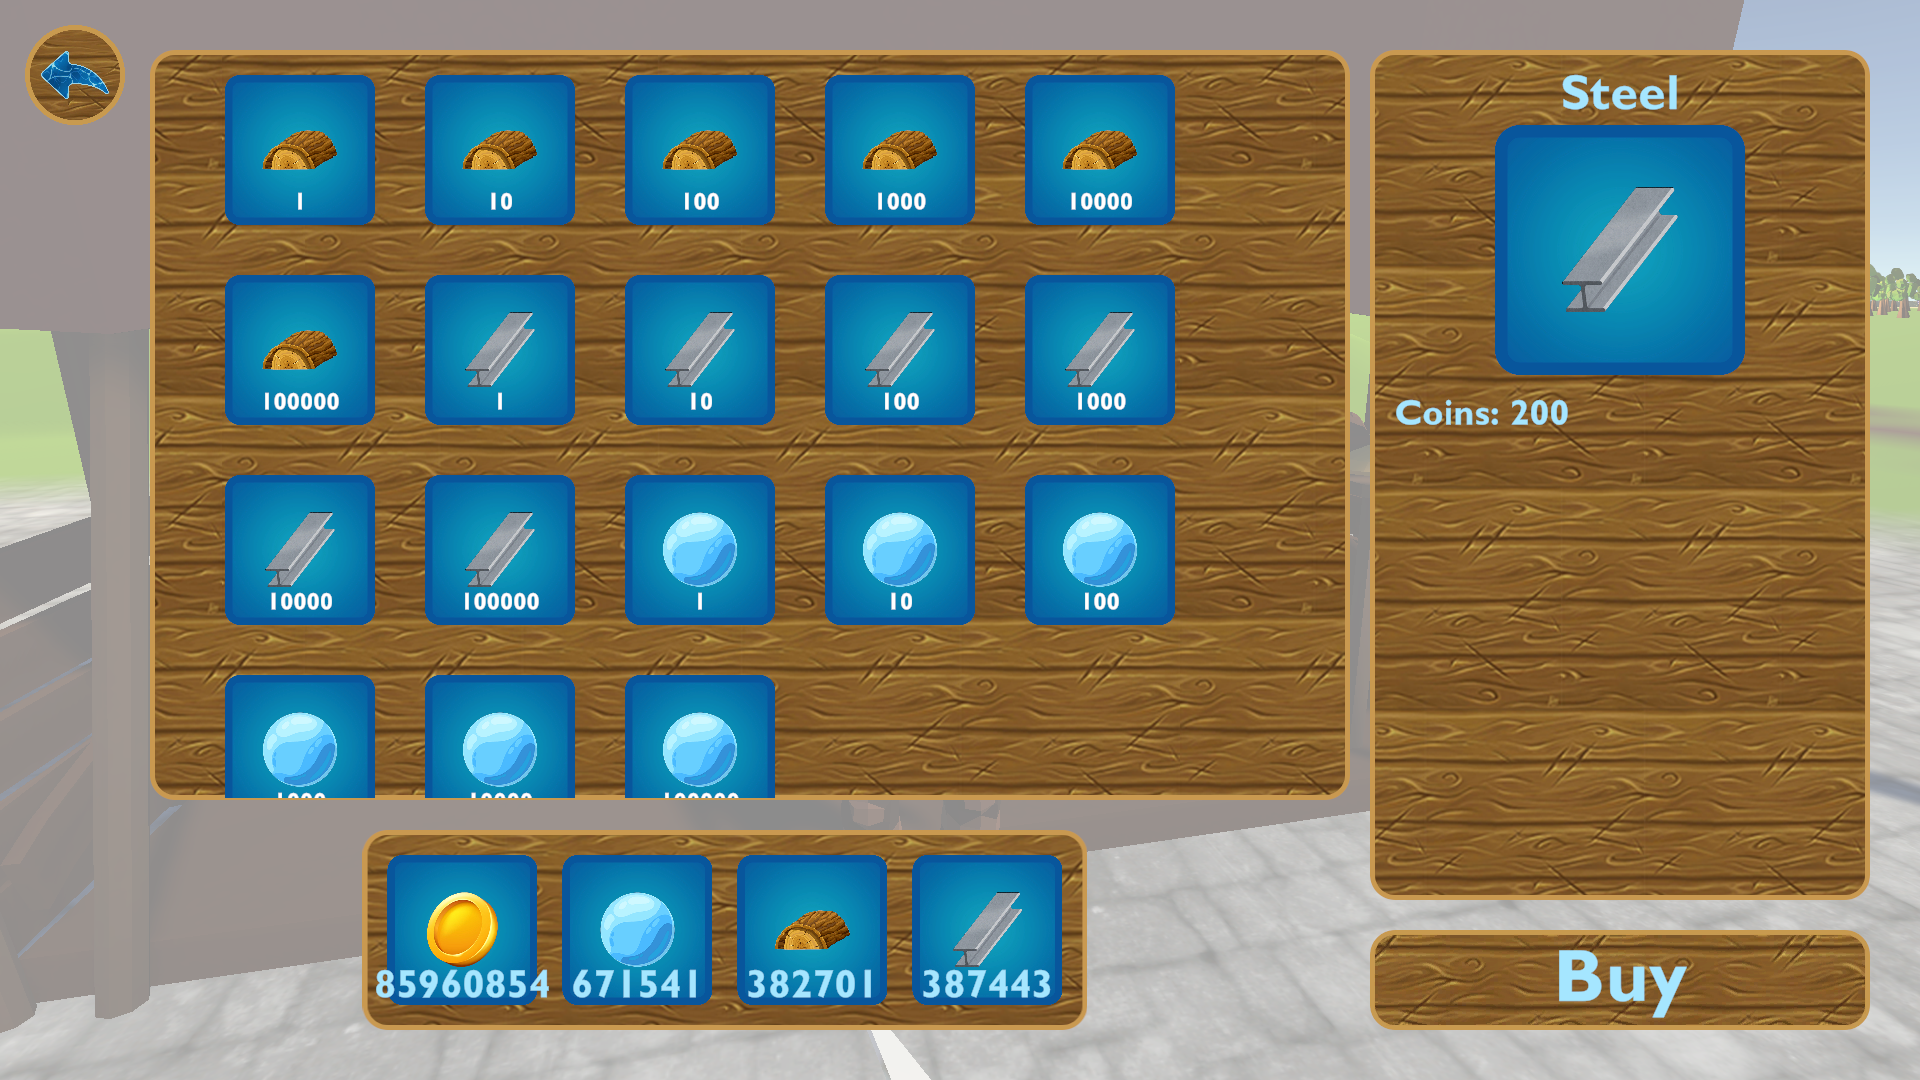
\includegraphics[width=5in]{Illustration/Shops/MaterialsSeller.png}
    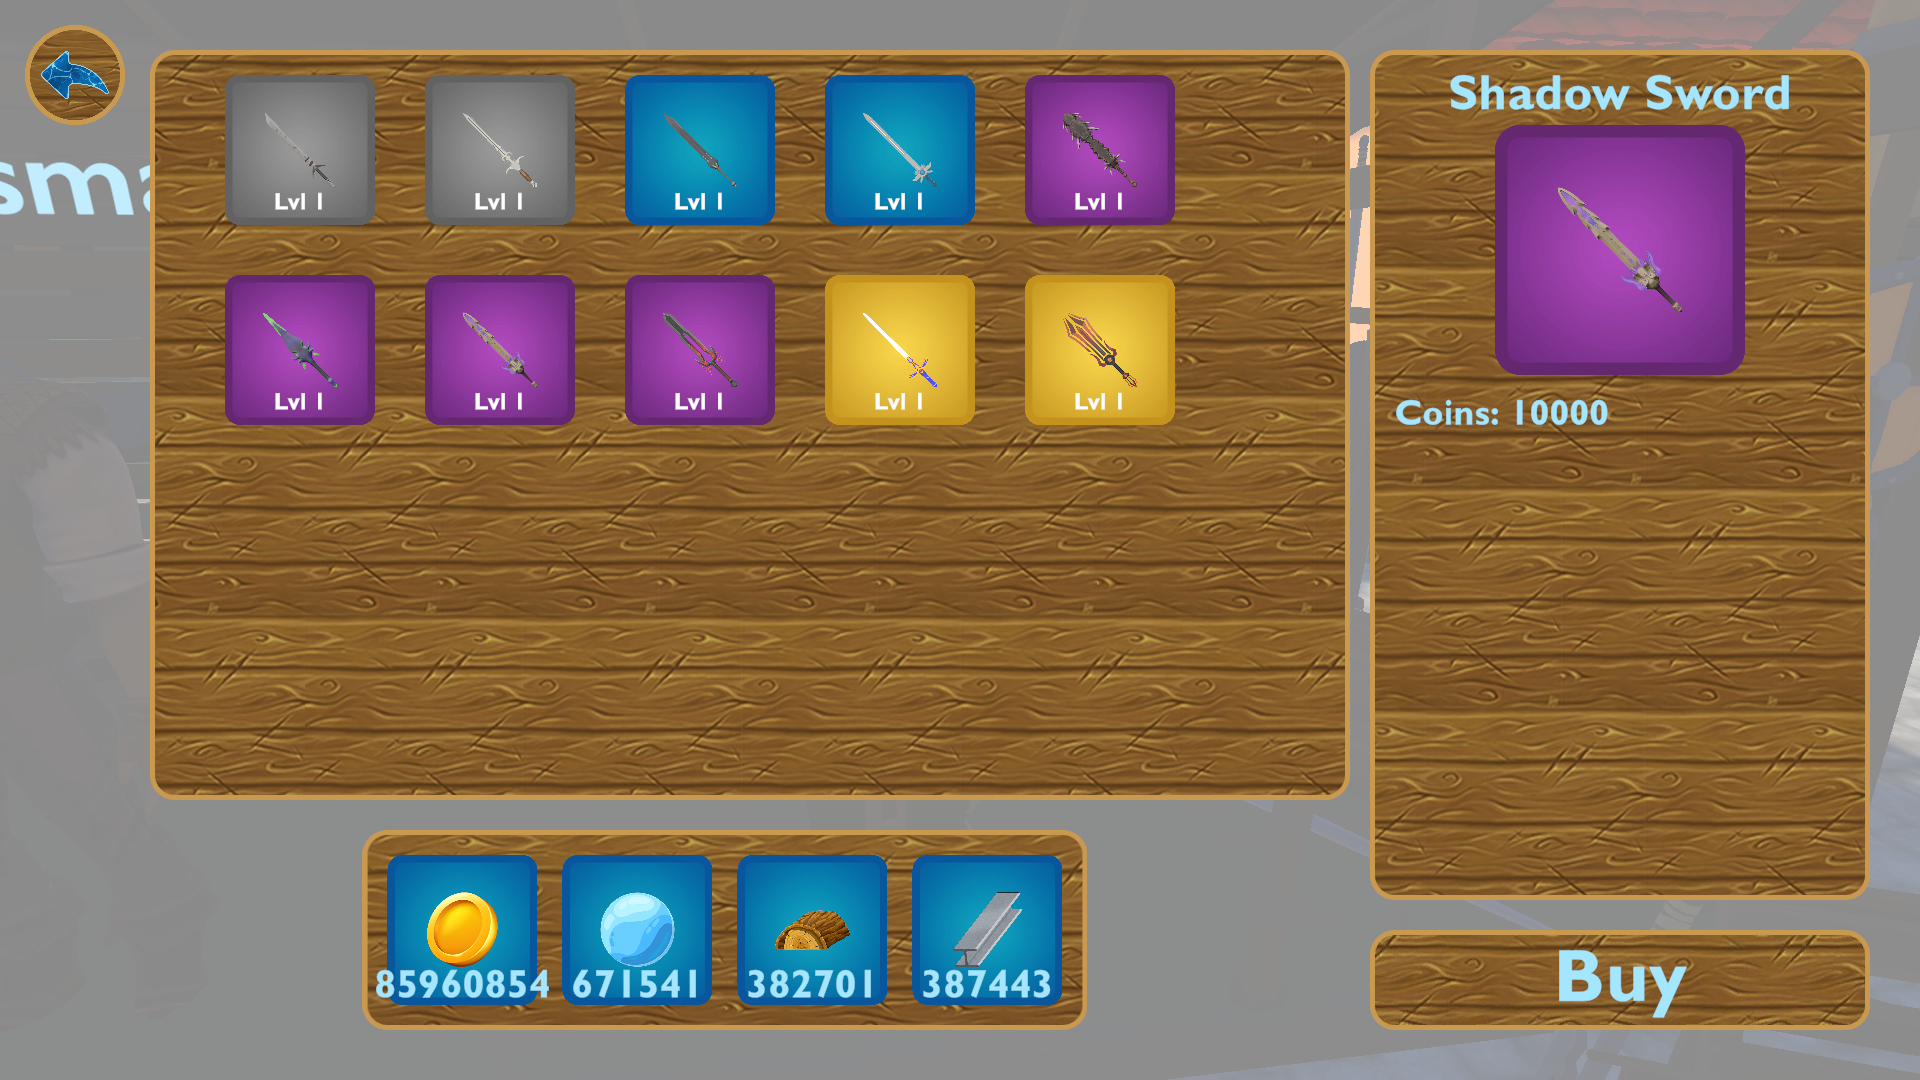
\includegraphics[width=5in]{Illustration/Shops/Armorer.png}
\end{center}

\subsection*{Fishing}
\begin{center}
    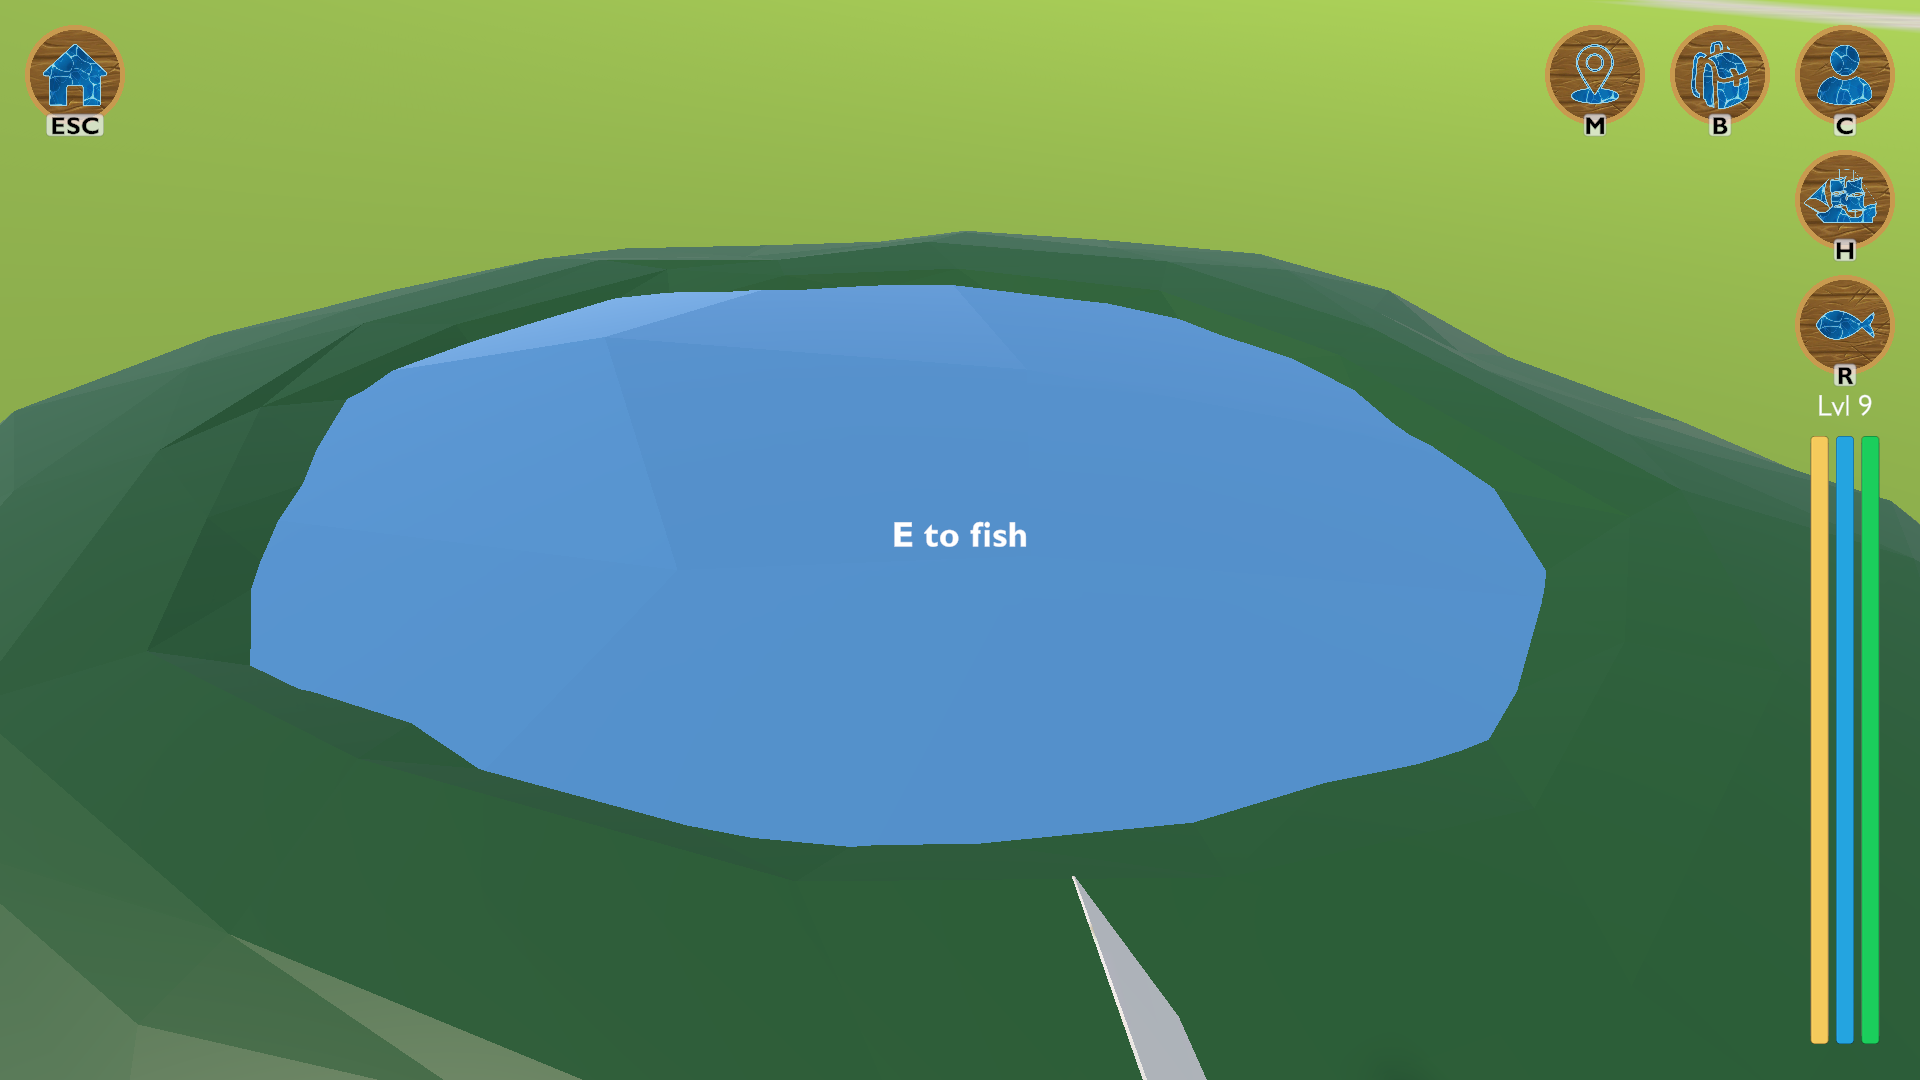
\includegraphics[width=5in]{Illustration/Fishing/Pond.png}
    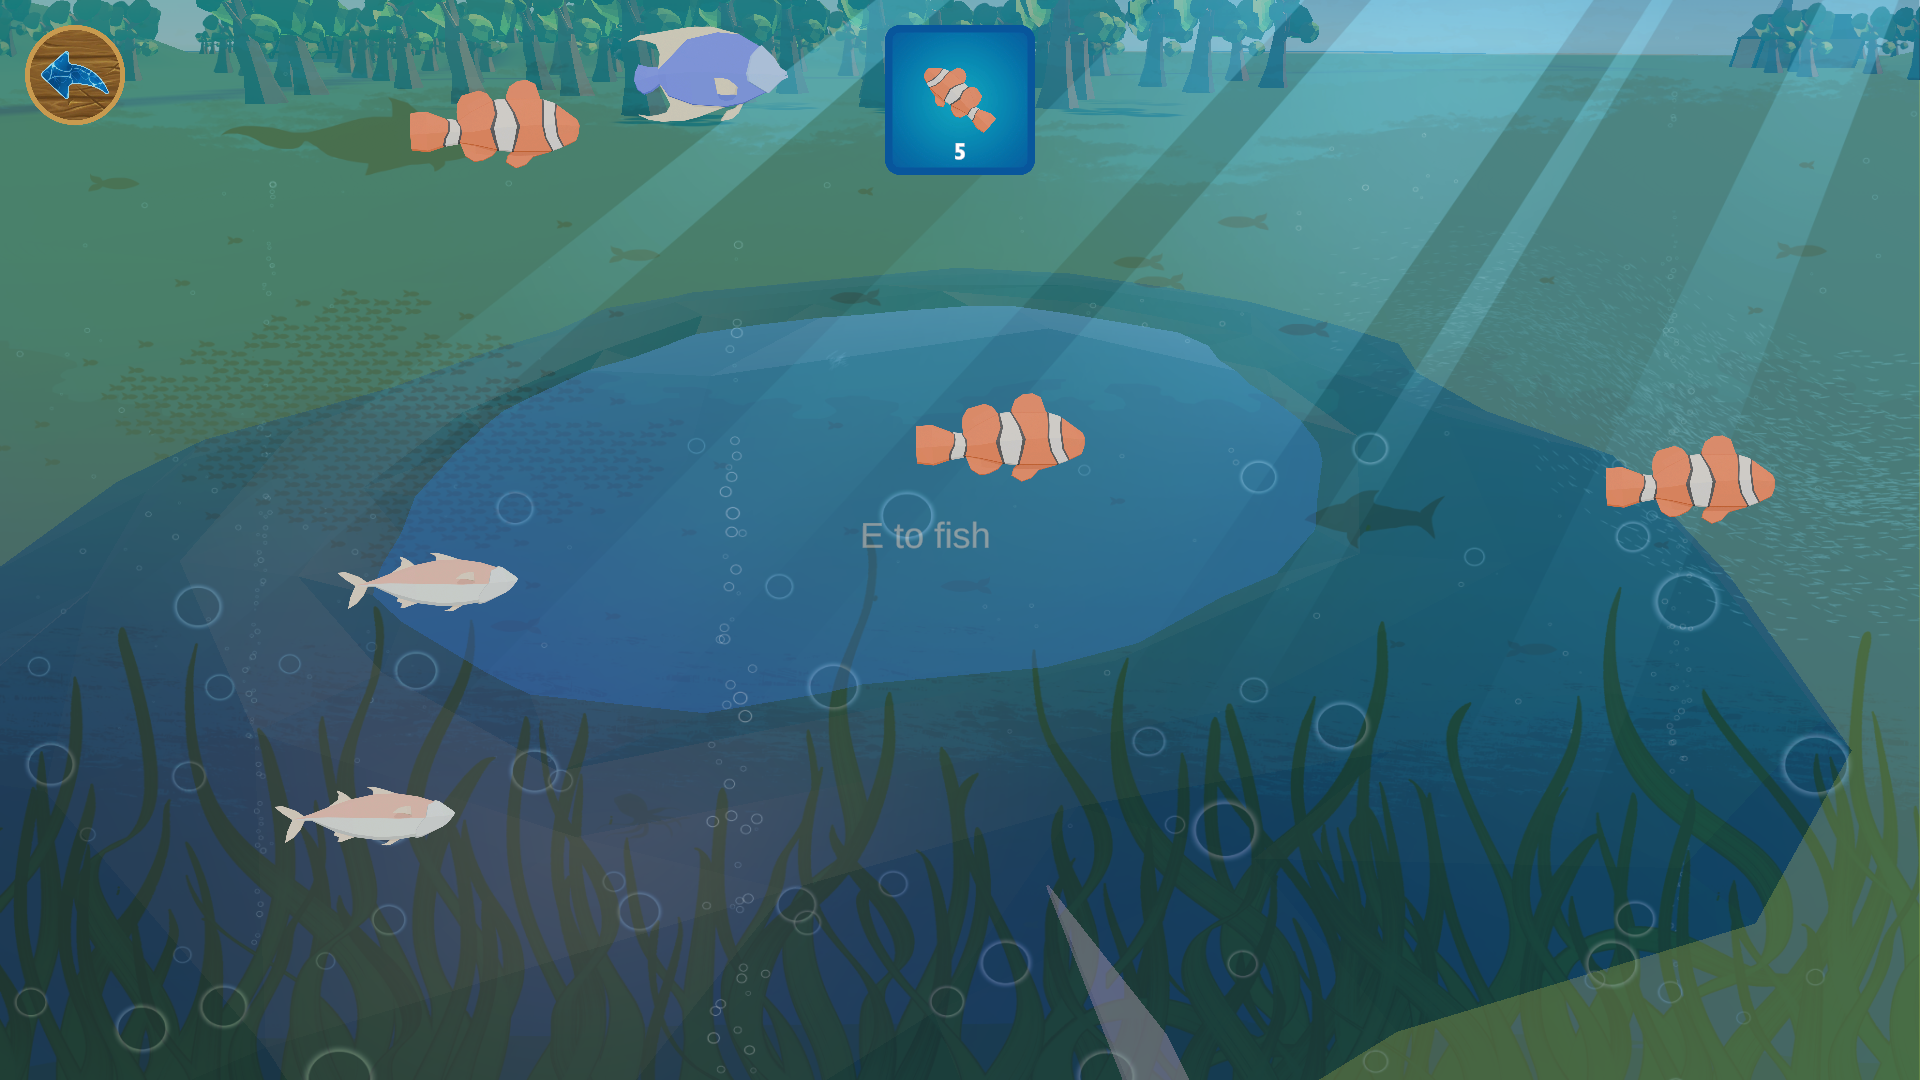
\includegraphics[width=5in]{Illustration/Fishing/Fishing.png}
\end{center}

\subsection*{Network}
\begin{center}
    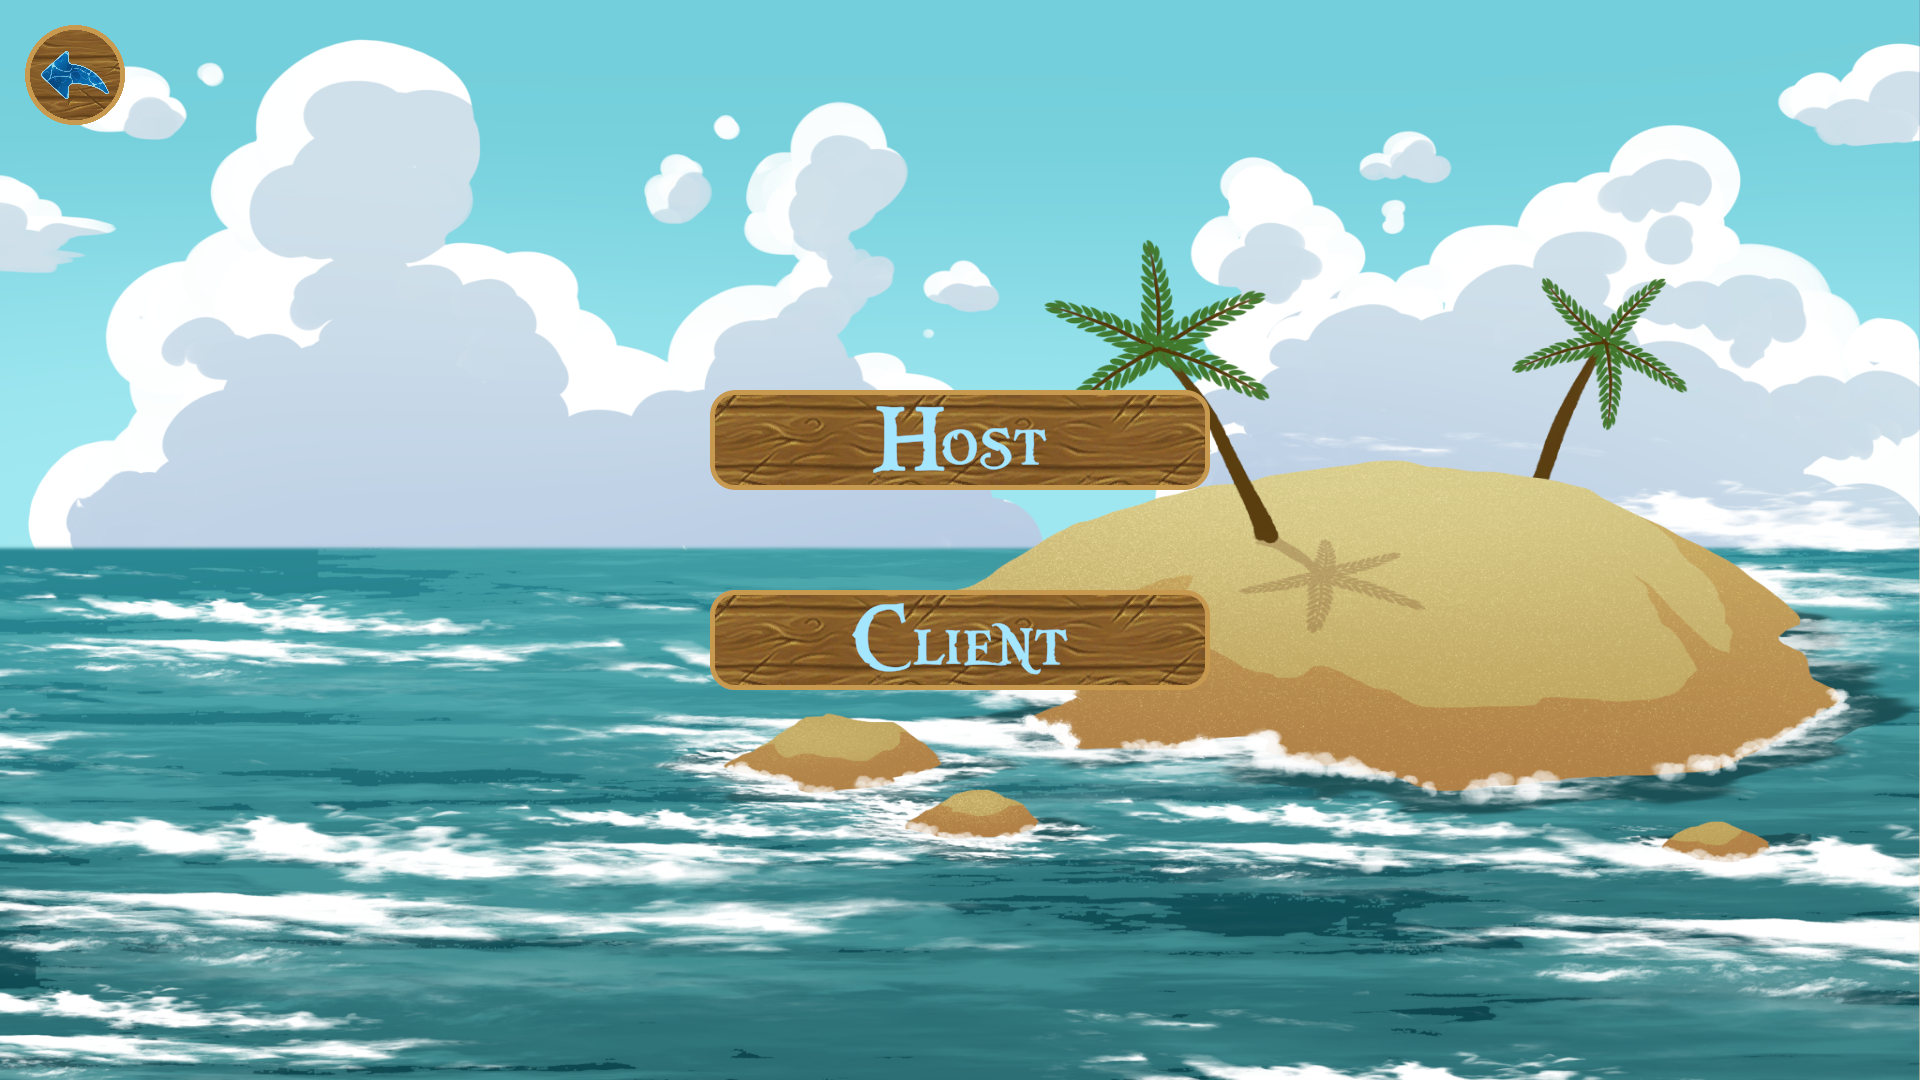
\includegraphics[width=5in]{Illustration/Network/MultiplayerHUD.png}
    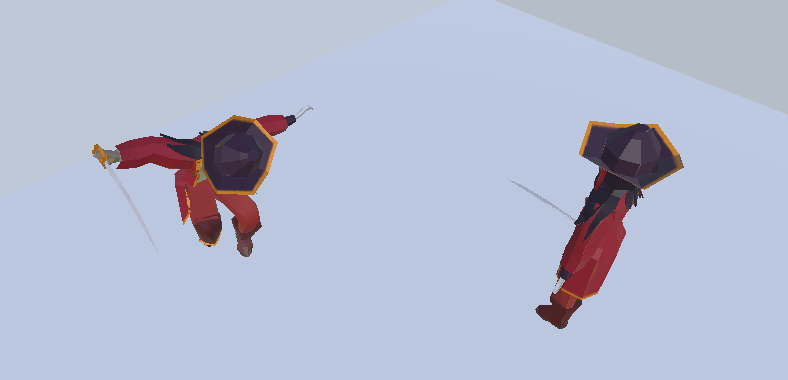
\includegraphics[width=5in]{Illustration/Network/NetworkPlayer.png}
\end{center}

\subsection*{Multiplayer}
\begin{center}
    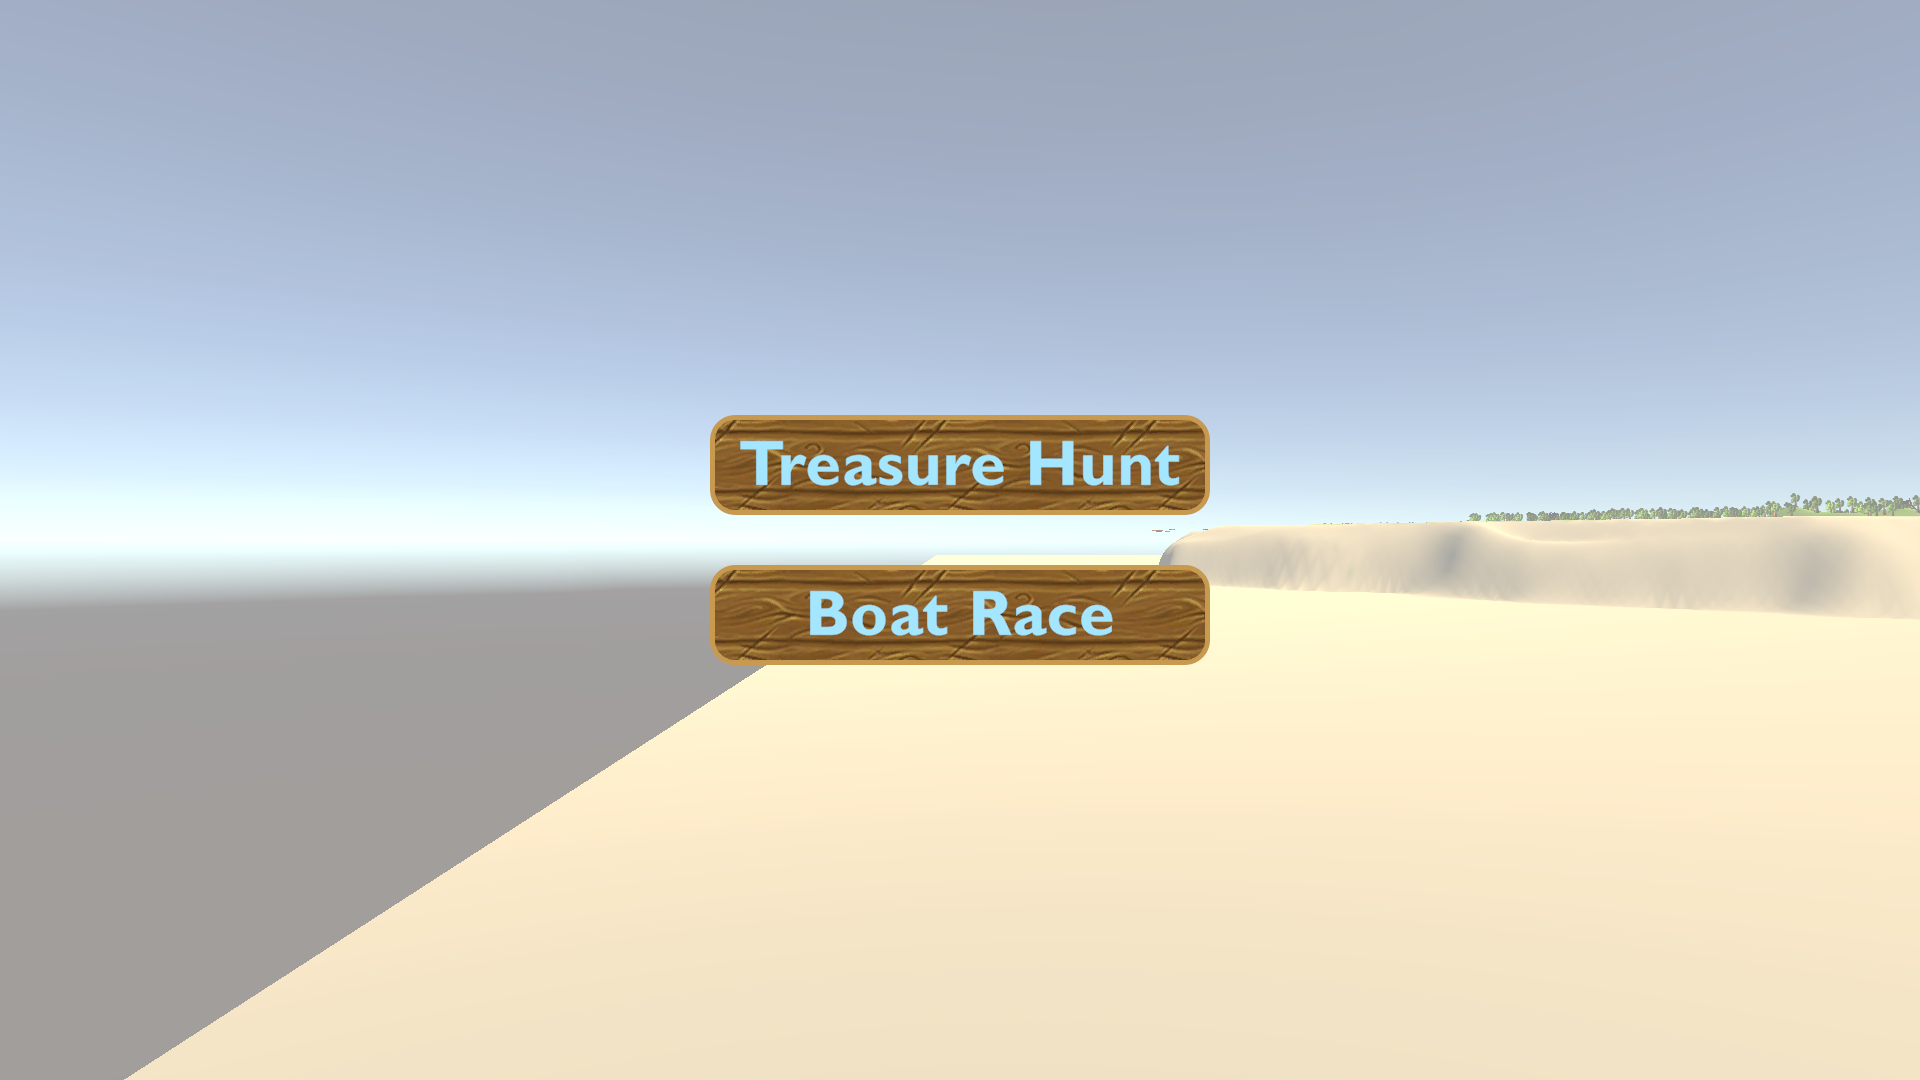
\includegraphics[width=5in]{Illustration/Multiplayer/MultiplayerChoiceModeMenu.png}
    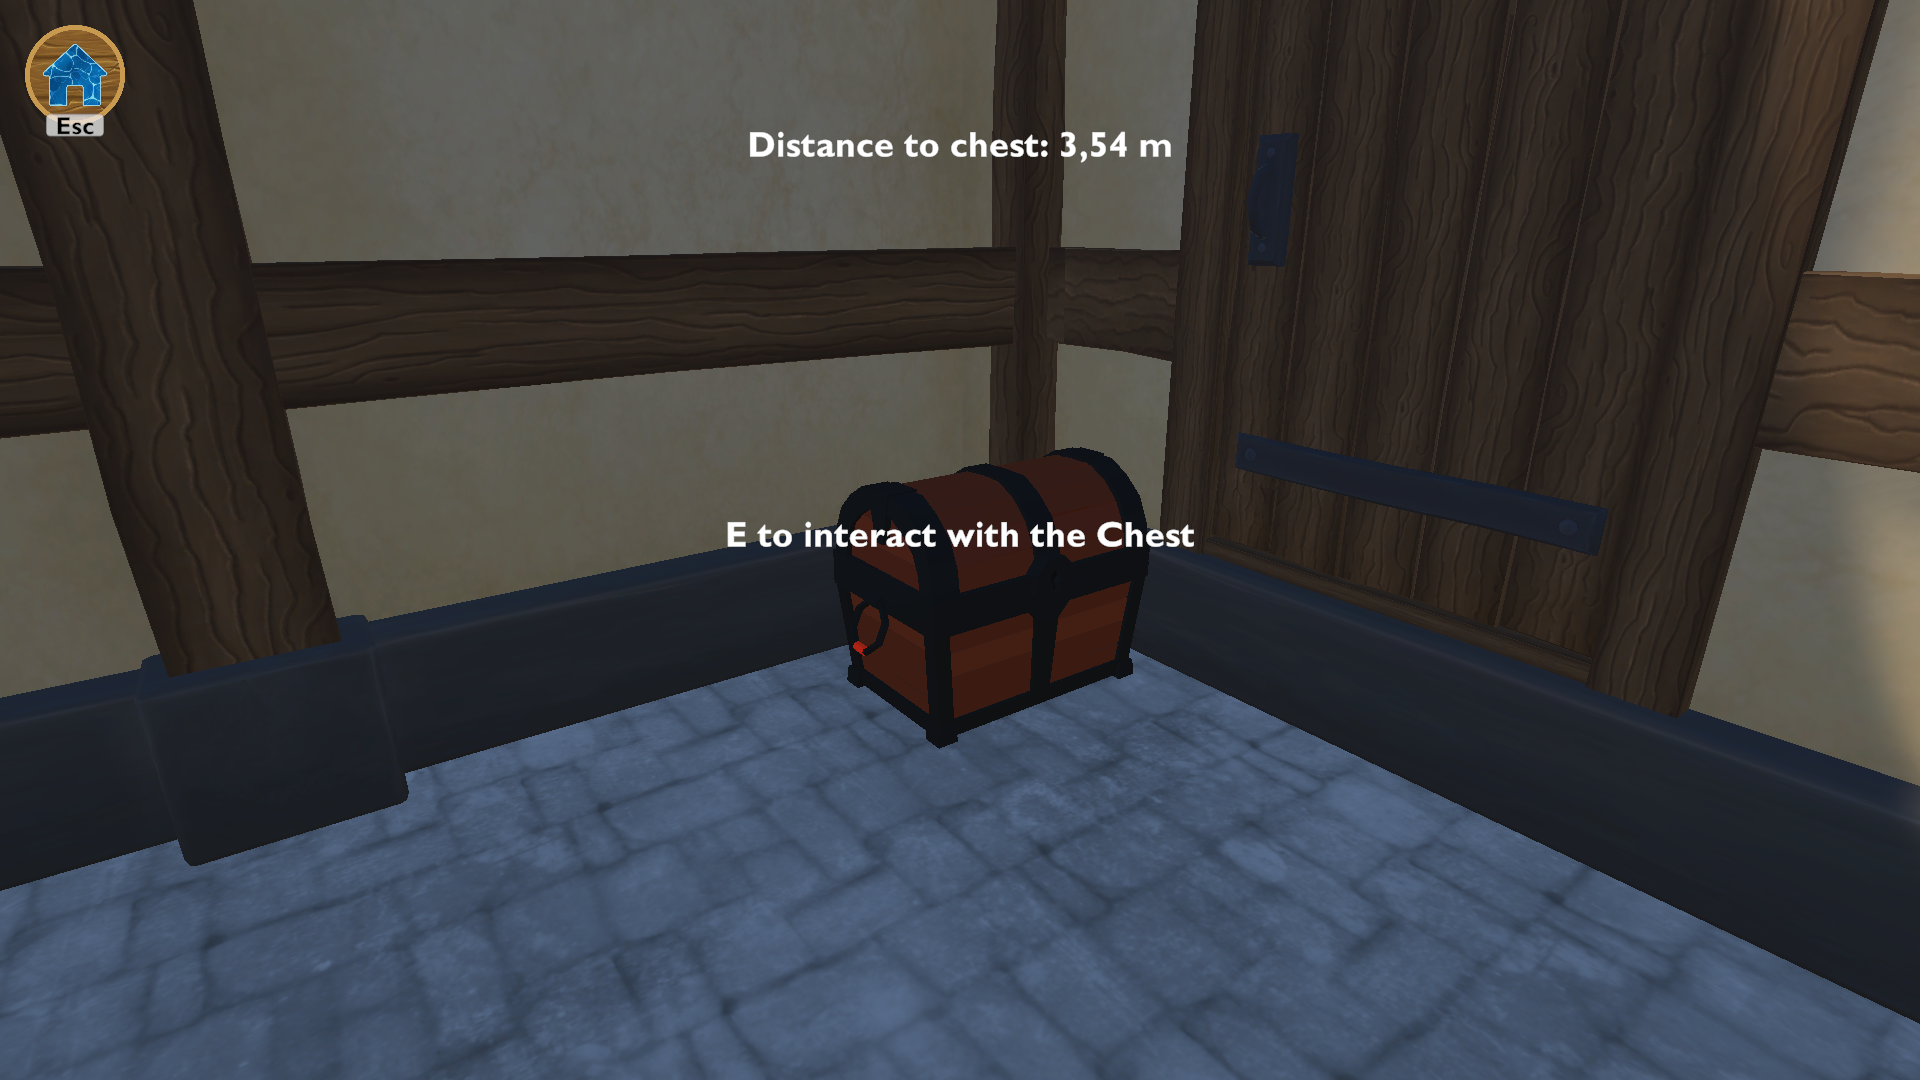
\includegraphics[width=5in]{Illustration/Multiplayer/TreasureHunt.png}
    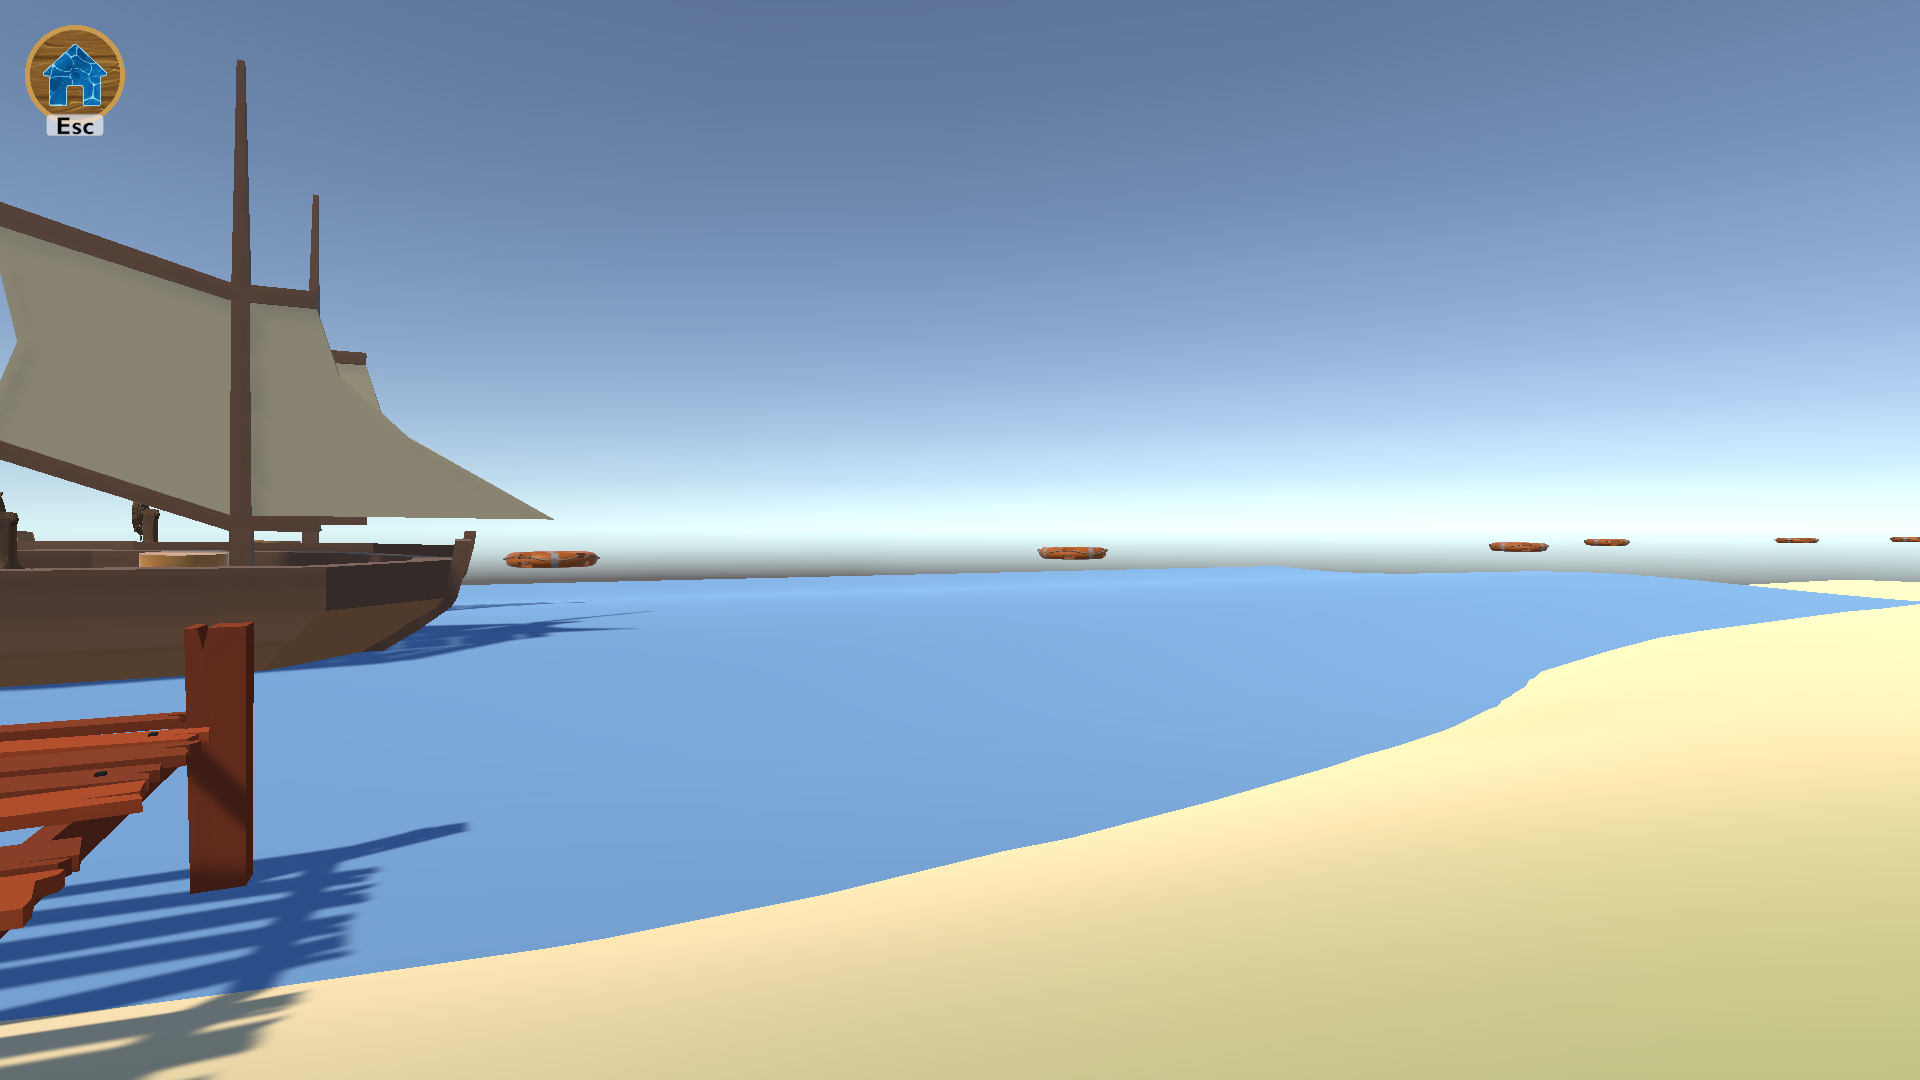
\includegraphics[width=5in]{Illustration/Multiplayer/BoatRace.png}
    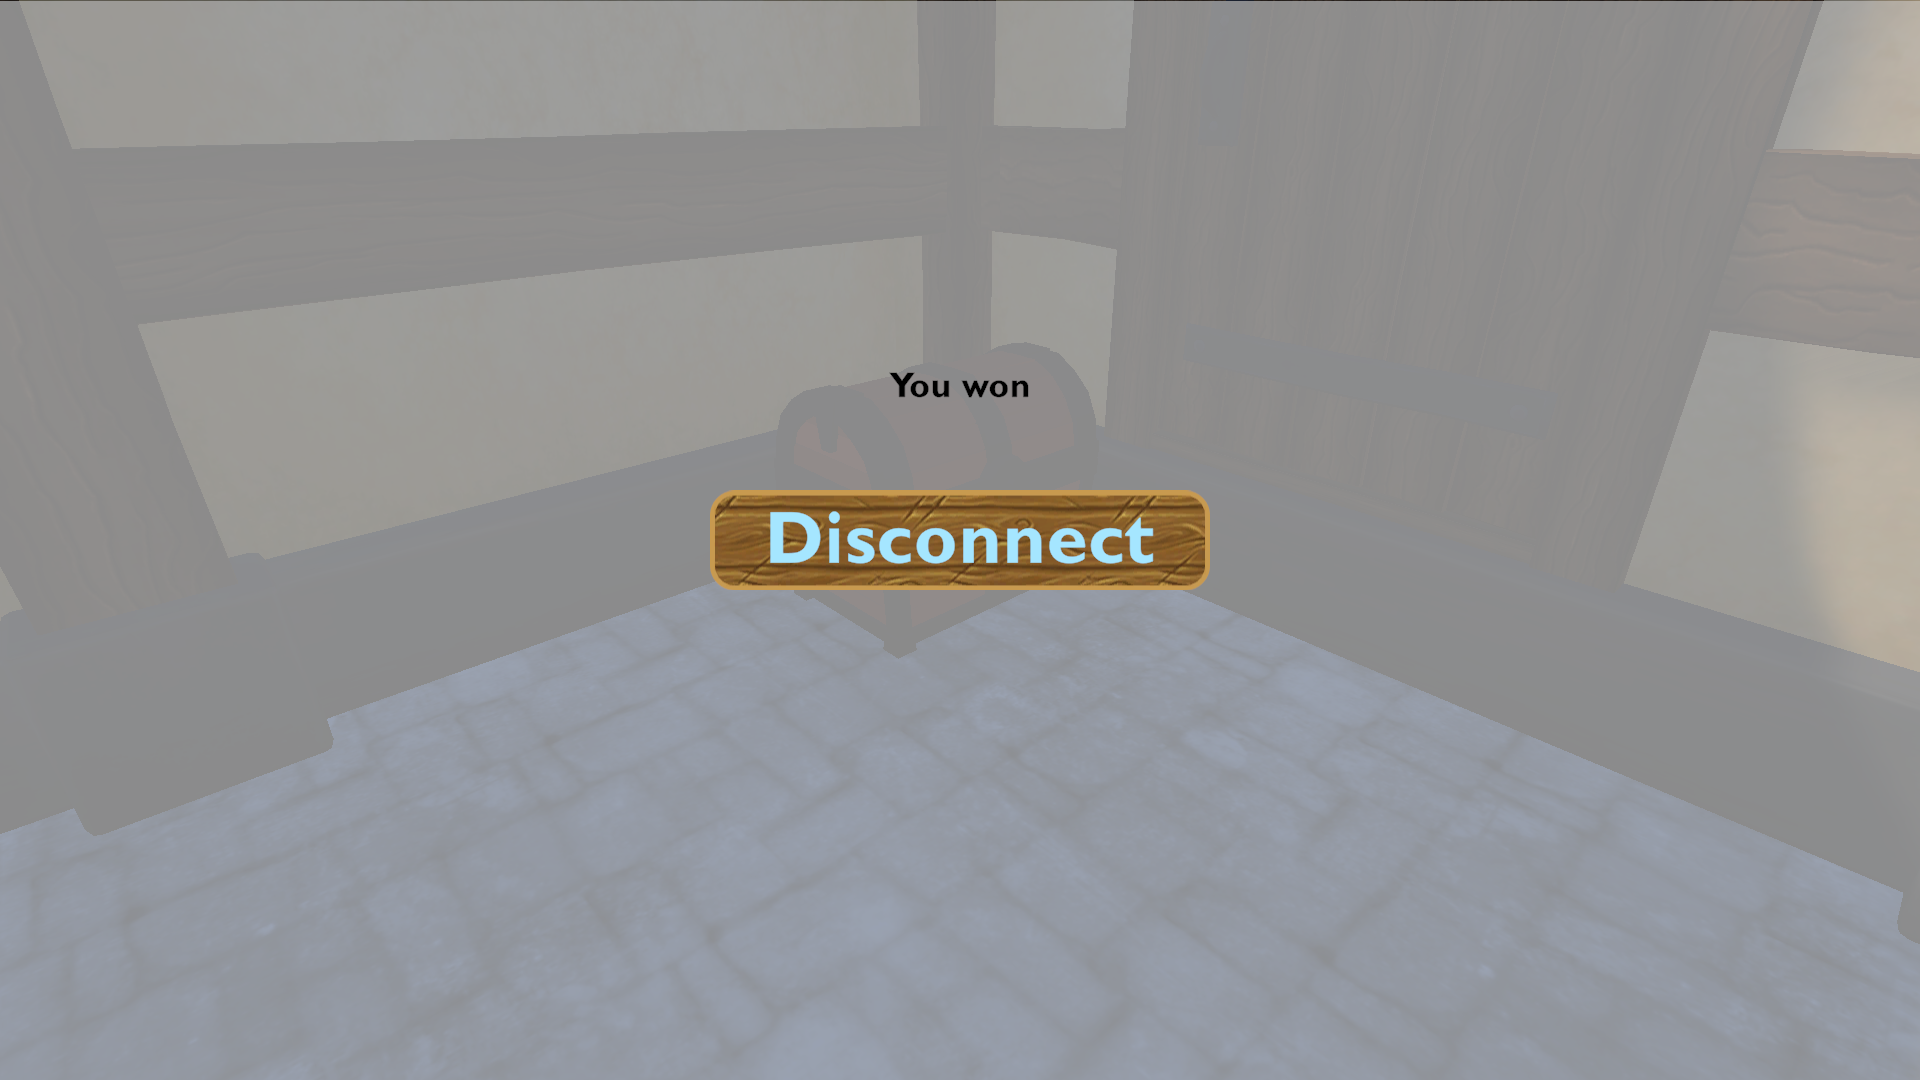
\includegraphics[width=5in]{Illustration/Multiplayer/MultiplayerResultMenu.png}
    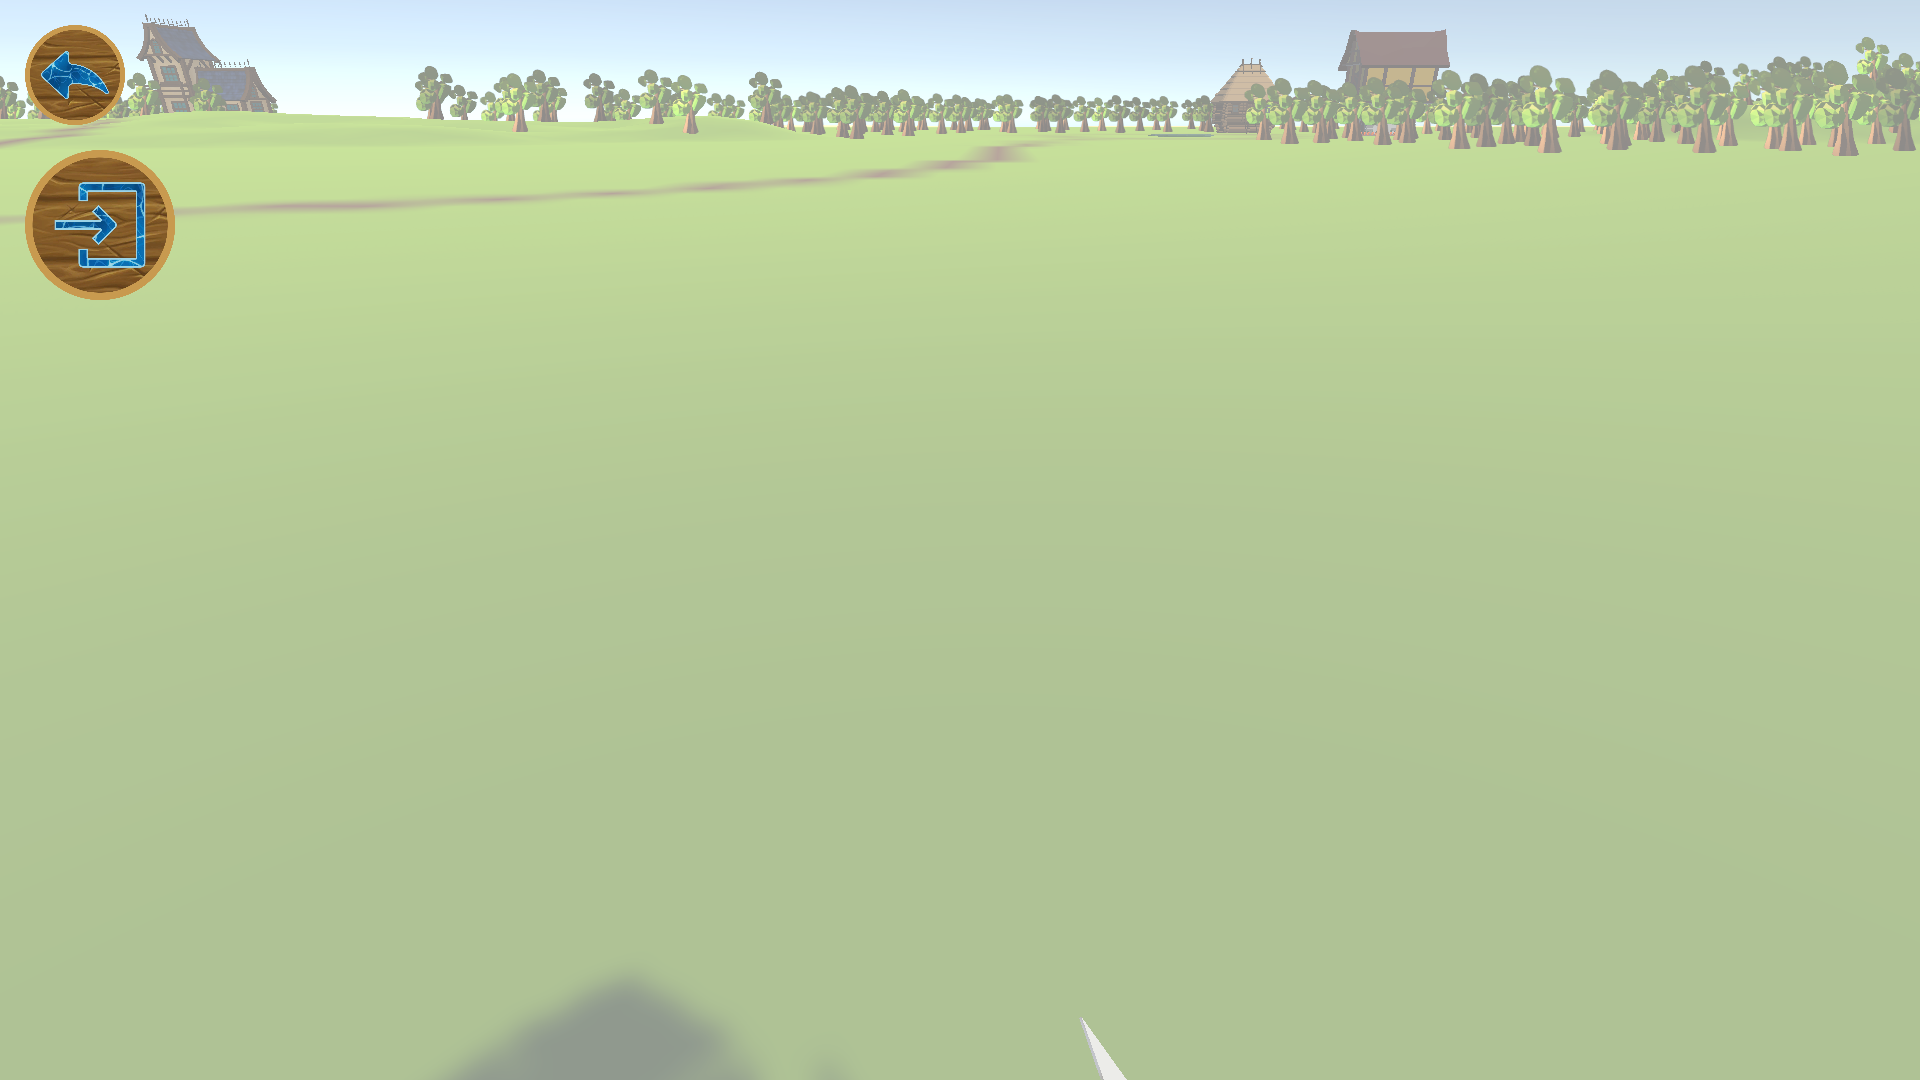
\includegraphics[width=5in]{Illustration/Multiplayer/Settings.png}
\end{center}

\subsection*{Quest}
\begin{center}
    
\includegraphics[width=5in]{Illustration/Quest/NPC.png}
    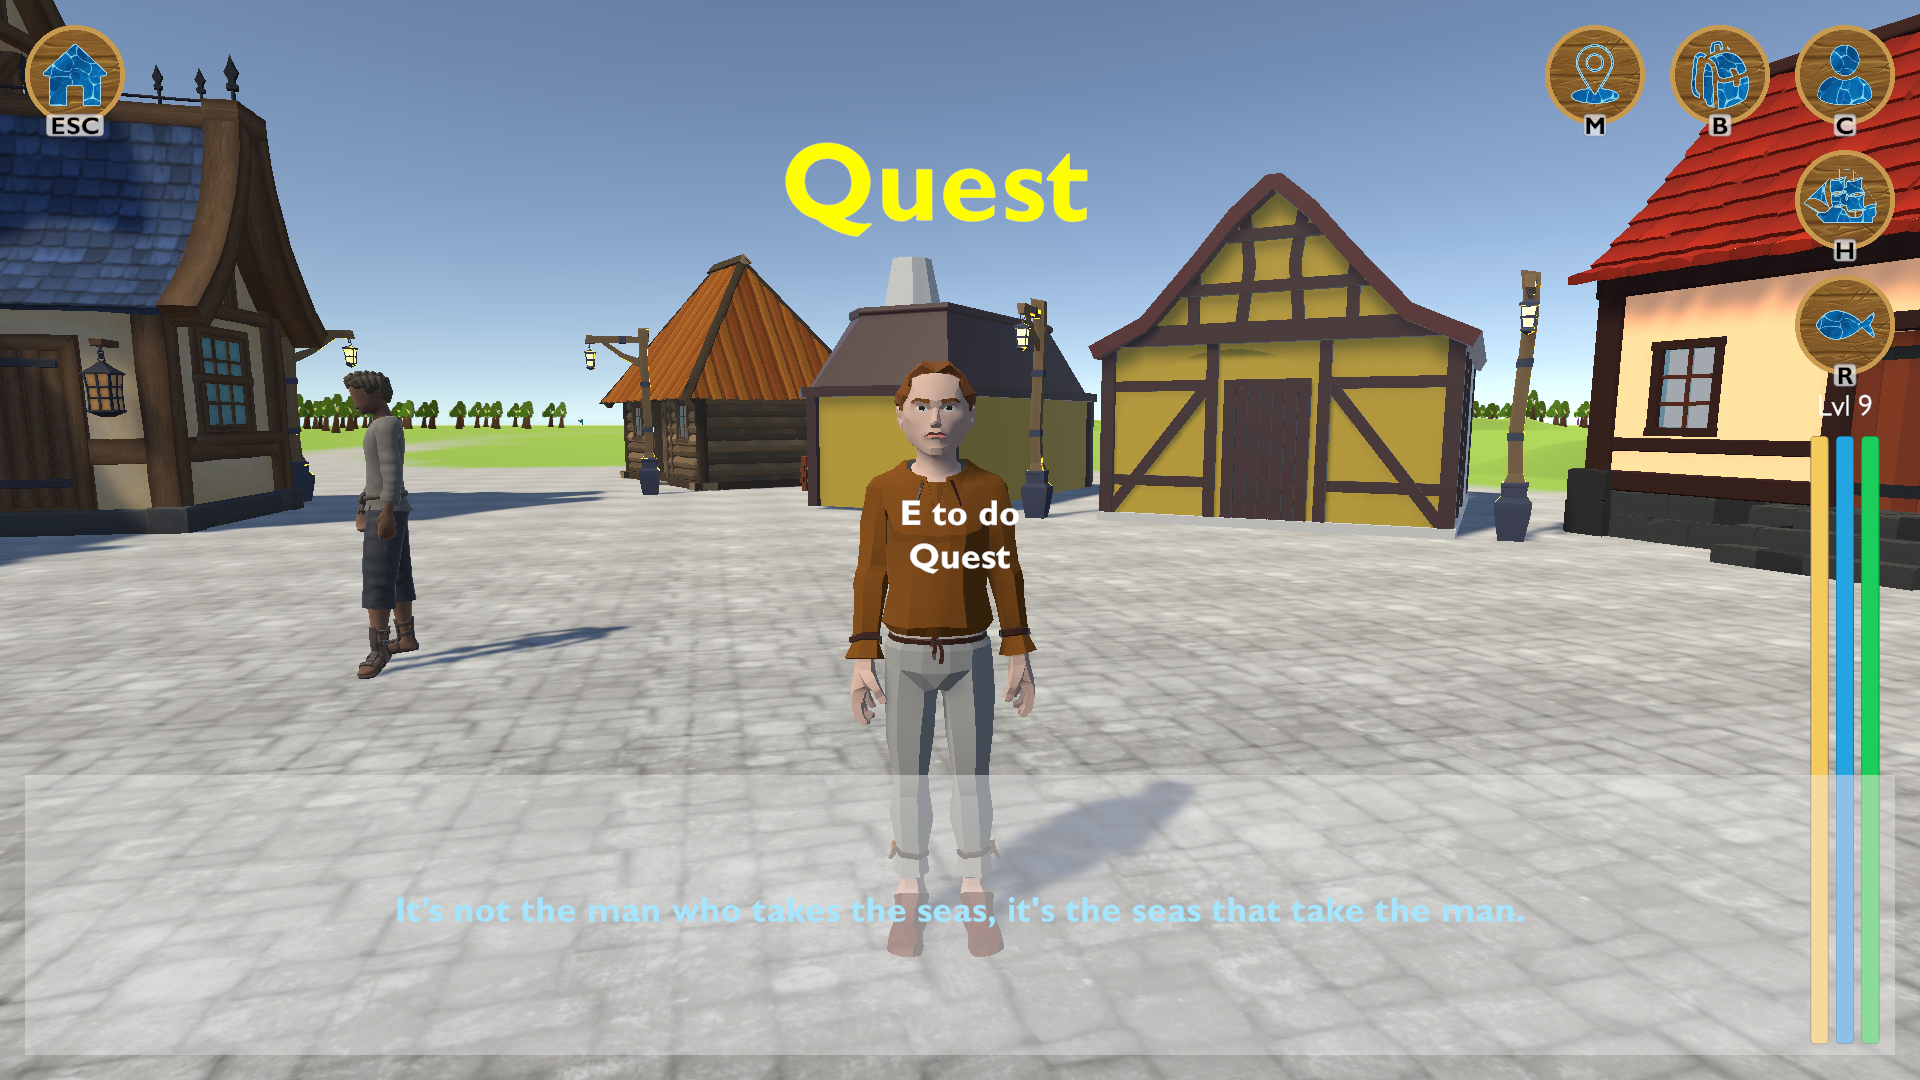
\includegraphics[width=5in]{Illustration/Quest/Dialogs.png}
\end{center}

\subsection*{Design Entities}
\begin{center}
    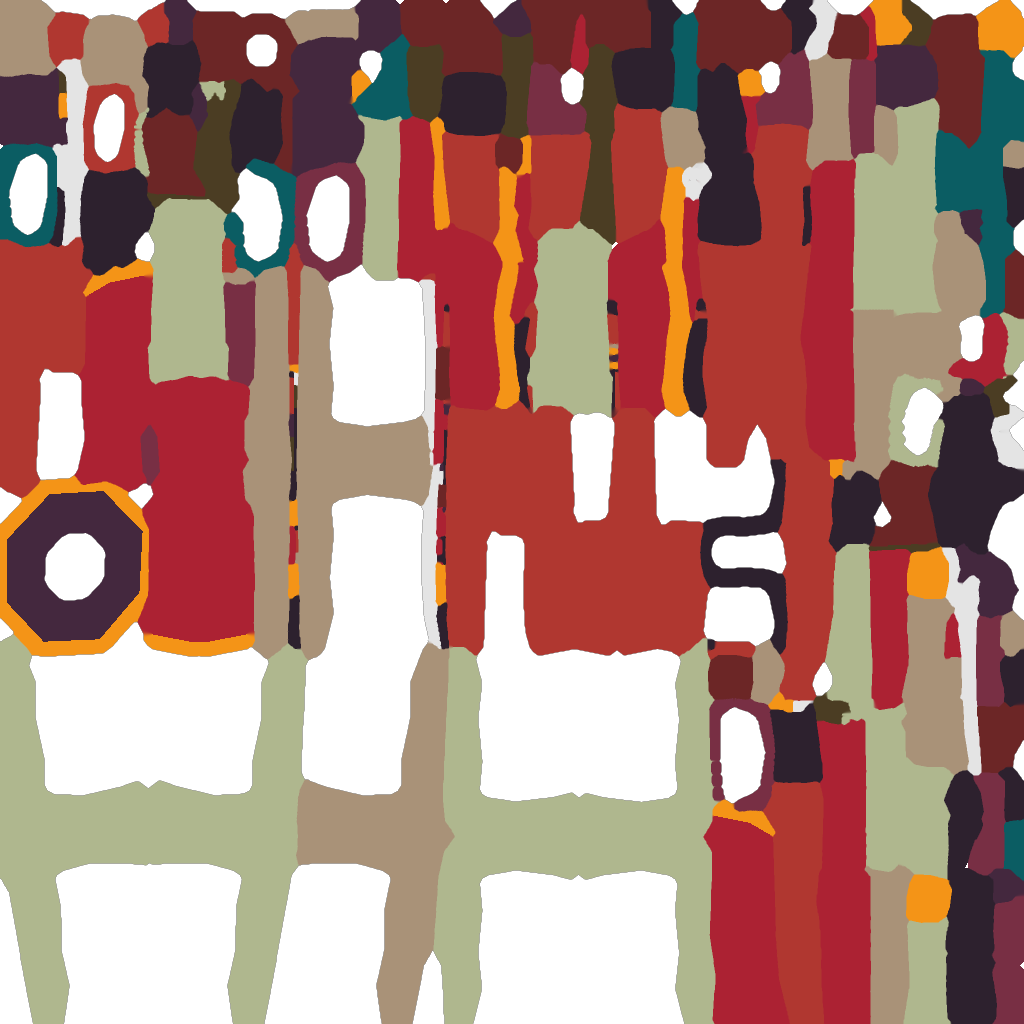
\includegraphics[width=3in]{Illustration/3DModel/Pirate1.png}
    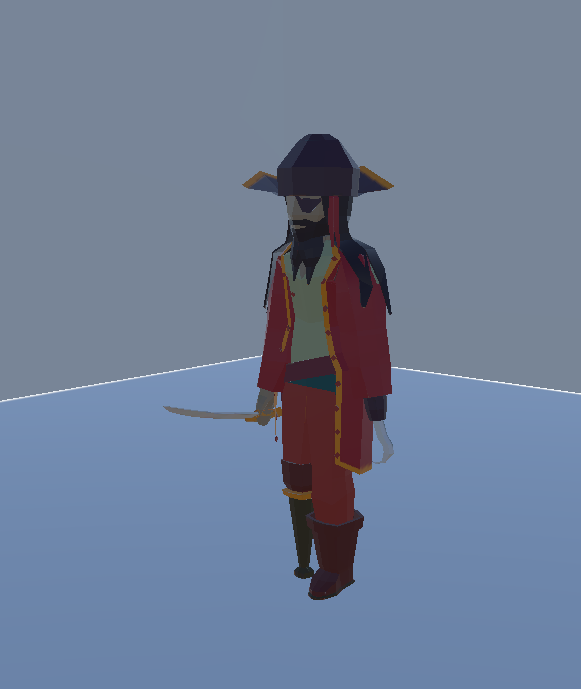
\includegraphics[width=3in]{Illustration/3DModel/Pirat.png}
    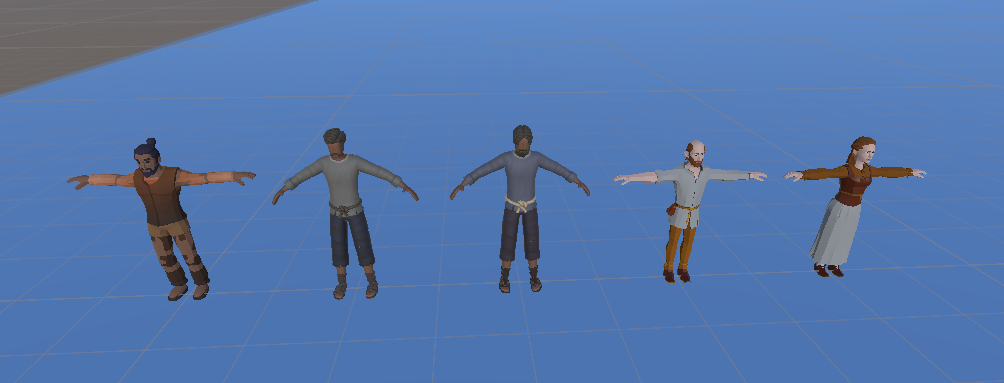
\includegraphics[width=5in]{Illustration/3DModel/NPC.png}
    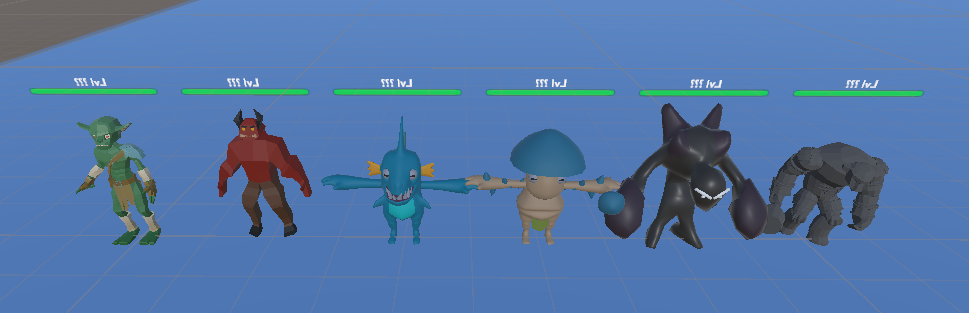
\includegraphics[width=5in]{Illustration/3DModel/TerestEnemies.png}
    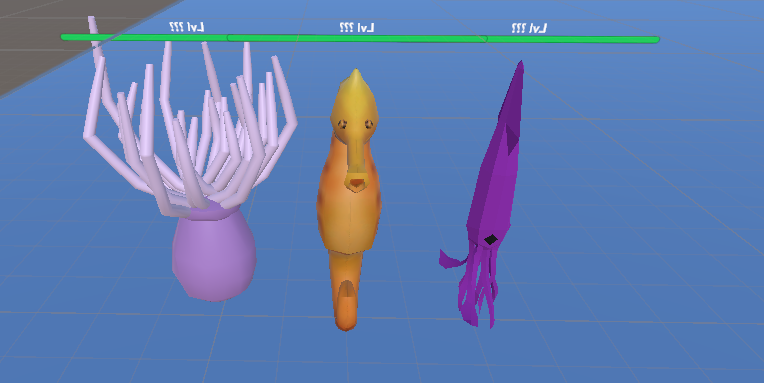
\includegraphics[width=5in]{Illustration/3DModel/MaritEnemies.png}
\end{center}















\end{document}